% !TEX program = xelatex
% Proyecto convertido desde DOCX a LaTeX.
% Recomendación de compilación: xelatex main.tex -> biber main -> xelatex main.tex -> xelatex main.tex
\documentclass[12pt,a4paper,oneside]{report}

% Idioma y tipografía
\usepackage[spanish,es-tabla]{babel}
\usepackage{fontspec}
% Todo el documento, excepto la carátula, usa Times New Roman 12 pt.
% Si Times New Roman no está instalado en el sistema de compilación, se usa Tinos
% como alternativa métrica compatible para permitir la generación del PDF.
\IfFontExistsTF{Times New Roman}
  {\setmainfont{Times New Roman}}
  {\IfFontExistsTF{Tinos}
    {\setmainfont{Tinos}}
    {\setmainfont{Latin Modern Roman}}}

\IfFontExistsTF{TeX Gyre Termes}
  {\newfontfamily\coverfont{TeX Gyre Termes}}
  {\IfFontExistsTF{Tinos}
    {\newfontfamily\coverfont{Tinos}}
    {\newfontfamily\coverfont{Latin Modern Roman}}}

% Usar solo newtxmath. Cargar newtxmath y unicode-math al mismo tiempo en XeLaTeX
% produce errores de redefinición (por ejemplo: \not=, \not< y \not>).
\usepackage{newtxmath}
\usepackage{newunicodechar}
\newunicodechar{≥}{\ensuremath{\geq}}
\newunicodechar{≤}{\ensuremath{\leq}}
\newunicodechar{×}{\ensuremath{\times}}
\newunicodechar{→}{\ensuremath{\rightarrow}}
\newunicodechar{•}{\textbullet}
\newunicodechar{–}{--}
\newunicodechar{—}{---}
\usepackage{csquotes}
\usepackage{microtype}
\usepackage{soulutf8}

% Márgenes y espaciado compatibles con APA 7
\usepackage[a4paper,margin=2.54cm]{geometry}
\usepackage{setspace}
\doublespacing
\setlength{\parindent}{1.27cm}
\setlength{\parskip}{0pt}

% Tablas, figuras y listas
\usepackage{graphicx}
\graphicspath{{./figuras/}{figuras/}{../figuras/}}
\usepackage{float}
\usepackage{booktabs}
\usepackage{longtable}
\usepackage{array}
\usepackage{tabularx}
\usepackage{calc}
\usepackage{enumitem}
\usepackage{caption}
\usepackage{chngcntr}
% Numeración consecutiva APA: Figura 1, Figura 2, Tabla 1, Tabla 2,
% sin anteponer el número del capítulo.
\counterwithout{figure}{chapter}
\counterwithout{table}{chapter}
\renewcommand{\thefigure}{\arabic{figure}}
\renewcommand{\thetable}{\arabic{table}}

% Formato APA 7 para tablas y figuras:
% número en negrita, título en cursiva en la línea siguiente y nota debajo.
% Según APA 7/UPC, la nota debe precisar si la tabla/figura es de elaboración propia,
% tomada o adaptada de una fuente externa.
\captionsetup{font=normalsize,labelfont=bf,labelsep=period}
\captionsetup[figure]{font=normalsize,labelfont=bf,textfont=it,labelsep=newline,justification=raggedright,singlelinecheck=false,skip=0.35em}
\captionsetup[table]{position=above,font=normalsize,labelfont=bf,textfont=it,labelsep=newline,justification=raggedright,singlelinecheck=false,skip=0.35em}
\renewcommand{\figurename}{Figura}
\renewcommand{\tablename}{Tabla}
% Nombres solicitados para índices preliminares
\AtBeginDocument{%
  \renewcommand{\contentsname}{Tabla de Contenido}%
  \renewcommand{\listtablename}{Lista de Tablas}%
  \renewcommand{\listfigurename}{Lista de Figuras}%
}
\addto\captionsspanish{%
  \renewcommand{\contentsname}{Tabla de Contenido}%
  \renewcommand{\listtablename}{Lista de Tablas}%
  \renewcommand{\listfigurename}{Lista de Figuras}%
}
\setlist[itemize]{leftmargin=*,topsep=0.3em}
\setlist[enumerate]{leftmargin=*,topsep=0.3em}

% Citas y referencias APA 7
\usepackage[style=apa,backend=biber,sortcites=true,sorting=nyt,natbib=false]{biblatex}
\DeclareLanguageMapping{spanish}{spanish-apa}
\addbibresource{references.bib}
% Ejemplos de uso APA 7:
% Cita narrativa: \textcite{bancomundial2024}
% Cita parentética: \parencite{bancomundial2024}
% Varias fuentes: \parencite{bancomundial2024,inei2024}

% Hipervínculos y referencias cruzadas
\usepackage{xurl}
\usepackage[hidelinks]{hyperref}
\usepackage[nameinlink,noabbrev]{cleveref}


% Formato de títulos: capítulos y secciones preliminares centrados

\def\chaptertitlefont{\normalfont\bfseries\normalsize}
\usepackage{titlesec}
\titleformat{\chapter}[display]
  {\chaptertitlefont\centering}
  {\chaptername\ \thechapter}
  {0.5em}
  {}
\titleformat{name=\chapter,numberless}[display]
  {\chaptertitlefont\centering}
  {}
  {0pt}
  {}
\titlespacing*{\chapter}{0pt}{0pt}{24pt}
% Todos los niveles de títulos se mantienen en 12 pt.
\titleformat{\section}{\normalfont\bfseries\normalsize}{\thesection}{0.6em}{}
\titleformat{\subsection}{\normalfont\bfseries\normalsize}{\thesubsection}{0.6em}{}
\titleformat{\subsubsection}{\normalfont\bfseries\normalsize}{\thesubsubsection}{0.6em}{}

% Título especial para Dedicatoria: alineado a la derecha
\newcommand{\dedicatoriatitle}{%
  \clearpage
  \phantomsection
  \addcontentsline{toc}{chapter}{Dedicatoria}%
  \begin{flushright}
    {\chaptertitlefont Dedicatoria}
  \end{flushright}
  \vspace{1.5em}
}

% Encabezados y numeración
\usepackage{fancyhdr}
\pagestyle{fancy}
\fancyhf{}
\fancyfoot[R]{\thepage}
\fancypagestyle{plain}{%
  \fancyhf{}%
  \fancyfoot[R]{\thepage}%
  \renewcommand{\headrulewidth}{0pt}%
}
\setlength{\headheight}{15pt}
\renewcommand{\headrulewidth}{0pt}
\setcounter{secnumdepth}{3}
\setcounter{tocdepth}{3}

% Comandos auxiliares
\providecommand{\tightlist}{\setlength{\itemsep}{0pt}\setlength{\parskip}{0pt}}
\newcommand{\pendiente}[1]{\textit{[PENDIENTE] #1}}
\newcommand{\placeholder}[1]{\textit{[Completar: #1]}}

% Nota APA para figuras. Reemplazar el contenido según corresponda:
% - Elaboración propia.
% - Tomado de \textit{Título}, por Autor/Institución, año, URL.
% - Adaptado de \textit{Título}, por Autor/Institución, año, URL.
\newcommand{\figurenote}[1]{%
  \par\vspace{0.35em}%
  \begin{minipage}{0.9\textwidth}%
  \singlespacing\normalsize\textit{Nota.} #1%
  \end{minipage}\par%
}

% Nota APA para tablas. En tablas creadas con booktabs/longtable puede usarse
% debajo de \bottomrule como una fila multicolumna adaptada al número de columnas.
% Ejemplo: \multicolumn{3}{p{0.94\textwidth}}{\tablenote{Elaboración propia.}}\\
\newcommand{\tablenote}[1]{\singlespacing\normalsize\textit{Nota.} #1}



% Paquetes auxiliares para tablas e imágenes generadas desde la última versión DOCX
\usepackage{multirow}
\usepackage{makecell}
\usepackage{adjustbox}
\usepackage{pdflscape}
\newunicodechar{✓}{\textsuperscript{v}}
\newunicodechar{✗}{\ensuremath{\times}}
\newunicodechar{∑}{\ensuremath{\sum}}
\newunicodechar{“}{``}
\newunicodechar{”}{''}
\newunicodechar{’}{'}
\newunicodechar{°}{\ensuremath{^\circ}}
\newunicodechar{–}{--}

\begin{document}
\pagenumbering{roman}

\begin{titlepage}
    \thispagestyle{empty}
    \centering
    \begingroup
    \coverfont
    \singlespacing
    \vspace*{-0.4cm}
    
\includegraphics[width=2.15cm]{figuras/docx_image1.jpg}\\[0.45cm]
    {\bfseries UNIVERSIDAD PERUANA DE CIENCIAS APLICADAS\\[0.45cm]}
    {FACULTAD DE INGENIERÍA\\[0.45cm]}
    {PROGRAMA ACADÉMICO DE INGENIERÍA DE SISTEMAS\\[0.75cm]}
    {Sistema de inteligencia regulatoria basado en IA generativa con arquitectura RAG para automatizar la interpretación de normas legales en una PYME farmacéutica minorista del Perú\\[1.05cm]}
    {\bfseries TESIS\\[0.45cm]}
    {Para optar el título profesional de Ingeniero de Sistemas\\[0.75cm]}
    {\bfseries AUTORES\\[0.35cm]}
    {Hervias Salas, Jadir Omar (0009-0009-4187-3880)\\[0.25cm]}
    {Mogollón Buitrón, Khail Andrés (0009-0008-6507-180X)\\[0.65cm]}
    {\bfseries ASESORES\\[0.35cm]}
    {Zacarías Ramos, Juan (0000-0003-2427-3938)\\[0.75cm]}
    {\bfseries Lima, mayo de 2026}
    \endgroup
\end{titlepage}

\tableofcontents
\clearpage
\listoftables
\clearpage
\listoffigures
\clearpage
\pagenumbering{arabic}
\setcounter{secnumdepth}{-1}
\section{1. Capítulo 1 -- Definición del
Proyecto}\label{capuxedtulo-1-definiciuxf3n-del-proyecto}

En el contexto actual, las micro y pequeñas empresas comerciales
peruanas enfrentan un entorno normativo dinámico y disperso. Una empresa
de este segmento debe atender obligaciones sanitarias, tributarias,
laborales, municipales y de protección al consumidor, muchas de las
cuales se publican o actualizan mediante normas, comunicados y
disposiciones de entidades como SUNAT, SUNAFIL, INDECOPI,
municipalidades y el Diario Oficial El Peruano. Esta situación es
crítica porque el desconocimiento o la interpretación tardía de una
obligación puede generar declaraciones fuera de plazo, pagos
incorrectos, multas, reprocesos administrativos y dependencia de
asesoría externa. En este marco, el proyecto toma como objeto de estudio
a Inversiones y Representaciones Peruanas LK S.R.L. (Boticas Farmaperu),
una PYME farmacéutica peruana que requiere mejorar su proceso de
identificación, interpretación y seguimiento de obligaciones normativas.
La elección de este tipo de organización permite construir una línea
base medible sobre tiempos de interpretación normativa, exactitud en la
identificación de obligaciones, dependencia de asesoría externa y
trazabilidad de las fuentes utilizadas para sustentar decisiones de
cumplimiento. En este capítulo se presenta la definición del problema,
el objeto de estudio, el campo de acción, la situación problemática y
los problemas específicos a resolver. Asimismo, se formulan los
objetivos del proyecto, los indicadores de éxito, la factibilidad
técnica y económica, y la propuesta preliminar del Sistema de
Inteligencia Regulatoria (SIR), el cual será desarrollado en los
capítulos posteriores.

\subsection{1.1 Definición del
Problema}\label{definiciuxf3n-del-problema}

El problema de investigación se centra en la baja capacidad operativa de
una PYME farmacéutica minorista para identificar, interpretar y
convertir cambios normativos en acciones concretas de cumplimiento. Esta
dificultad no se limita a la existencia de normas complejas, sino que se
manifiesta en un proceso manual, disperso y dependiente de personas
externas, donde la empresa revisa múltiples portales, interpreta
disposiciones legales con lenguaje técnico y registra sus obligaciones
en hojas de cálculo o mensajes internos sin trazabilidad suficiente. La
relevancia del problema se sustenta en la importancia de las MYPE dentro
de la estructura empresarial peruana. PRODUCE informó que al cierre de
2024 el Perú registró 2,346,592 empresas formales, de las cuales el 99.1
\% correspondió a micro y pequeñas empresas; además, el sector comercio
representó el 44.2 \% del total de MYPE formales y las MYPE concentraron
el 86.5 \% del empleo privado (Ministerio de la Producción, 2025). Esta
concentración convierte al subsector comercio en un escenario pertinente
para validar una solución RegTech orientada a reducir la carga de
cumplimiento normativo.

\subsubsection{1.1.1 Objeto de Estudio}\label{objeto-de-estudio}

El objeto de estudio del proyecto es Inversiones y Representaciones
Peruanas LK S.R.L. (Boticas Farmaperu), una PYME farmacéutica minorista
ubicada en Lima Metropolitana y dedicada a la venta minorista de
productos farmacéuticos, dispositivos médicos, productos sanitarios,
productos de cuidado personal y artículos de botica. La empresa
pertenece al segmento de pequeña empresa, se encuentra acogida al
Régimen MYPE Tributario, cuenta con 10 trabajadores, registra ventas
anuales aproximadas de S/ 960,000 y desarrolla operaciones mediante tres
locales de atención al público en Santa Anita. La selección de una PYME
farmacéutica minorista se justifica por tres razones. Primero, el
comercio es el sector con mayor participación entre las MYPE formales
del país, lo que incrementa la representatividad del caso. Segundo, una
PYME farmacéutica minorista tiene obligaciones frecuentes ante SUNAT,
SUNAFIL, DIGEMID/MINSA, INDECOPI y municipalidades, lo que permite
construir un entorno de cumplimiento verificable. Tercero, el proceso de
interpretación normativa puede medirse con instrumentos simples: tiempo
de búsqueda, precisión en la identificación de obligaciones, número de
fuentes revisadas, costo de asesoría externa y satisfacción del usuario
final.

\textbf{Perfil de la organización:}

\phantomsection\label{_Toc231672256}{}Tabla 1\\
\emph{Perfil del objeto de estudio}

\begin{longtable}[]{@{}
  >{\raggedright\arraybackslash}p{(\columnwidth - 2\tabcolsep) * \real{0.4696}}
  >{\raggedright\arraybackslash}p{(\columnwidth - 2\tabcolsep) * \real{0.5304}}@{}}
\toprule\noalign{}
\begin{minipage}[b]{\linewidth}\raggedright
Elemento
\end{minipage} & \begin{minipage}[b]{\linewidth}\raggedright
Descripción
\end{minipage} \\
\midrule\noalign{}
\endhead
\bottomrule\noalign{}
\endlastfoot
RUC & 20607397164 \\
Razón social & Inversiones y Representaciones Peruanas LK S.R.L. \\
Nombre comercial & Boticas Farmaperu \\
Tipo de empresa & Pequeña empresa farmacéutica minorista peruana. \\
Ubicación & Santa Anita, Lima Metropolitana. \\
Cantidad de locales & 3 locales de atención al público en Santa
Anita. \\
Actividad económica & Venta minorista de productos farmacéuticos,
dispositivos médicos, productos sanitarios, productos de cuidado
personal y artículos de botica. \\
Régimen tributario & Régimen MYPE Tributario. SUNAT señala que este
régimen fue creado para micro y pequeñas empresas y exige condiciones
más simples para el cumplimiento de obligaciones tributarias
(Superintendencia Nacional de Aduanas y de Administración Tributaria,
2026b). \\
Tamaño operativo & 10 trabajadores distribuidos en tres locales de
atención al público en Santa Anita, considerando personal de atención en
botica, administración, dirección técnica farmacéutica y apoyo contable
externo. \\
Áreas involucradas & Gerencia general, administración, contabilidad
externa, recursos humanos y atención en botica. \\
Entes regulatorios principales & SUNAT, SUNAFIL, DIGEMID/MINSA,
INDECOPI, Municipalidad Distrital y Diario Oficial El Peruano como
fuente normativa. \\
\end{longtable}

\textbf{Misión:}

Brindar productos de uso cotidiano para pacientes, familias y vecinos
del distrito de Santa Anita mediante sus tres locales de atención y
canales de comunicación con clientes, garantizando una atención
confiable, precios competitivos y cumplimiento responsable de las
obligaciones tributarias, laborales y comerciales aplicables.

\textbf{Visión:}

Ser una cadena local de boticas formal, segura y digitalmente
organizada, reconocida en Santa Anita por su atención responsable,
trazabilidad documental y cumplimiento oportuno de la normativa
sanitaria y empresarial peruana aplicable.

\textbf{Objetivos organizacionales vinculados al proyecto:}

\begin{itemize}
\item
  Reducir el tiempo invertido por la administración y la contabilidad
  externa en la búsqueda e interpretación de cambios normativos.
\item
  Mejorar la trazabilidad de las fuentes utilizadas para tomar
  decisiones de cumplimiento.
\item
  Disminuir el riesgo de incumplimientos sanitarios, tributarios,
  laborales, municipales y de protección al consumidor.
\item
  Fortalecer la gestión documental y el seguimiento interno de
  obligaciones recurrentes y eventuales.
\end{itemize}

\textbf{Macroprocesos:}

Los macroprocesos de Inversiones y Representaciones Peruanas LK S.R.L.
(Boticas Farmaperu) se organizan en procesos estratégicos, operativos y
de soporte. La problemática del proyecto se manifiesta principalmente en
el macroproceso de soporte denominado gestión administrativa y
cumplimiento normativo, debido a que desde este proceso se revisan
disposiciones legales, se coordinan declaraciones tributarias, se
gestionan obligaciones laborales y se responde a requerimientos de
entidades regulatorias. La Figura 1 presenta el mapa de procesos
propuesto y resalta el proceso donde se ubica la problemática.

\phantomsection\label{_Toc231672401}{}Figura 1\\
\emph{Mapa de procesos}

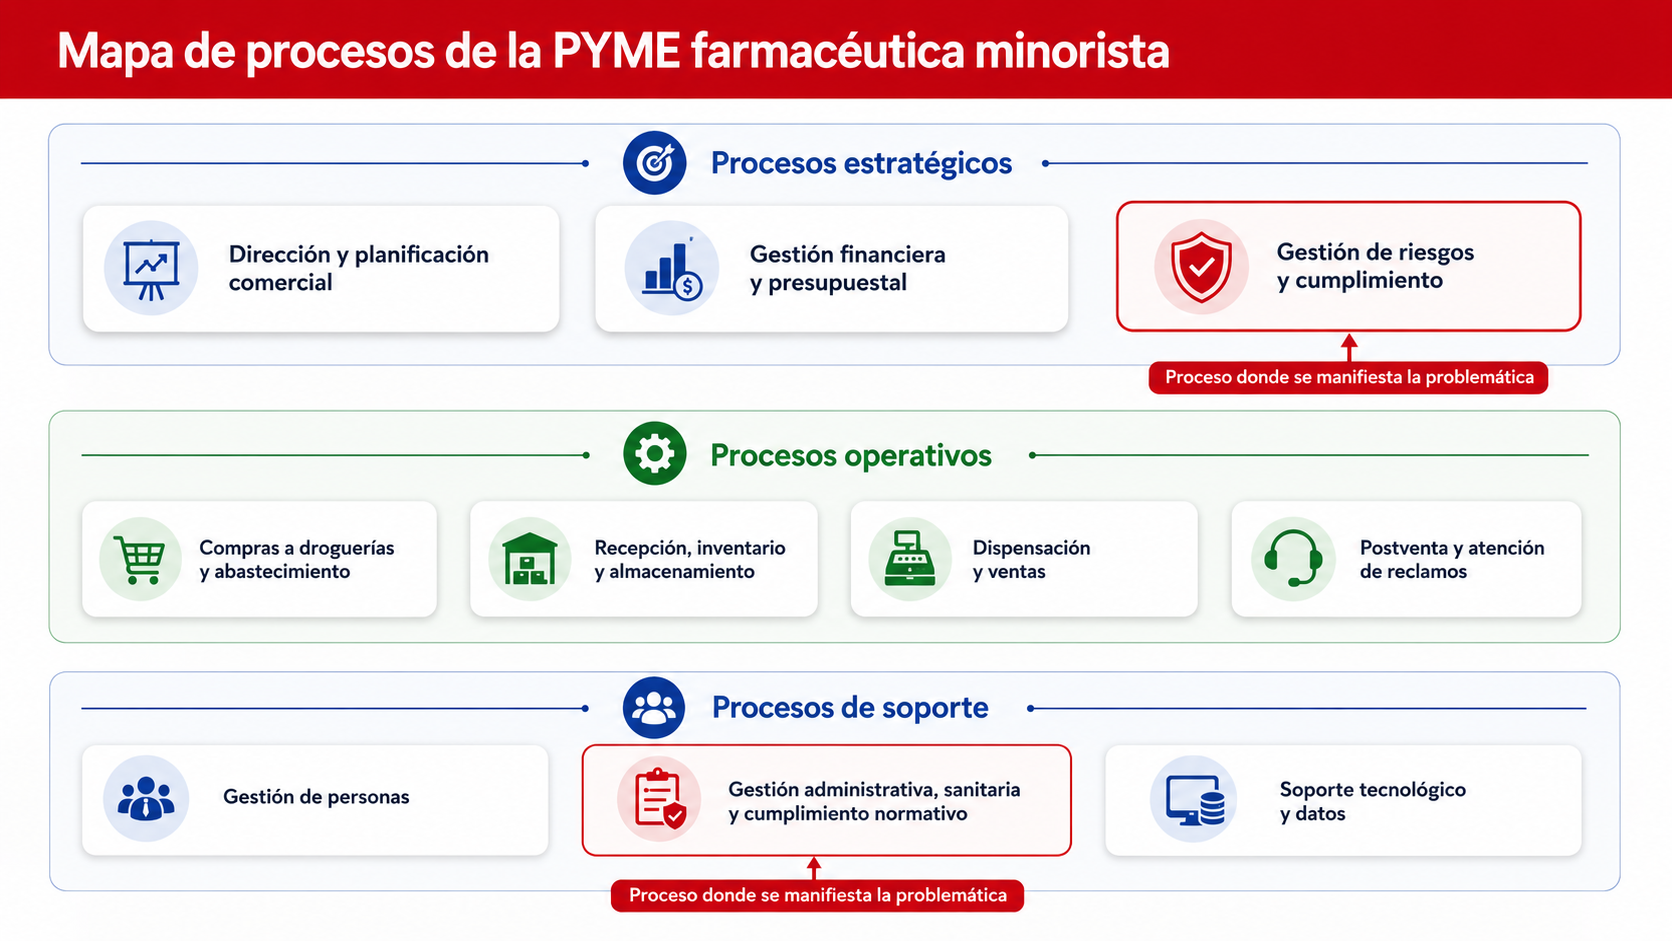
\includegraphics[width=6.5in,height=3.65625in]{figuras/docx_image3.png}

\subsubsection{1.1.2 Campo de acción}\label{campo-de-acciuxf3n}

El campo de acción corresponde al proceso de gestión administrativa y
cumplimiento normativo de Inversiones y Representaciones Peruanas LK
S.R.L. (Boticas Farmaperu). Este proceso comprende la identificación de
normas aplicables, interpretación de obligaciones, asignación de
responsables, registro de evidencias y seguimiento del cumplimiento ante
entidades regulatorias. El alcance no incluye la emisión de asesoría
legal vinculante, sino la generación de orientación operativa trazable
para que la PYME pueda comprender qué debe revisar, qué acción debe
ejecutar y qué fuente oficial sustenta la recomendación.

\textbf{Proceso AS-IS de cumplimiento normativo:}

\begin{enumerate}
\def\labelenumi{\arabic{enumi}.}
\item
  La administradora o el contador externo revisa manualmente fuentes
  como SUNAT, SUNAFIL, INDECOPI, municipalidad, Diario Oficial El
  Peruano y correos de notificación.
\item
  Se identifica si una norma, comunicado o requerimiento puede aplicar a
  la empresa según rubro, tamaño, número de trabajadores, ventas y canal
  de venta.
\item
  La información se interpreta manualmente y se consulta al contador o
  asesor externo cuando el lenguaje técnico no es claro.
\item
  Las tareas de cumplimiento se registran en hojas de cálculo, correos o
  mensajes de WhatsApp sin un repositorio único de trazabilidad.
\item
  La empresa ejecuta la acción correspondiente: declaración, pago,
  actualización documental, respuesta a requerimiento, corrección de
  comprobantes, actualización del Libro de Reclamaciones o revisión
  laboral.
\end{enumerate}

\textbf{Sistemas y fuentes involucradas:}

\phantomsection\label{_Toc231672257}{}Tabla 2\\
\emph{Sistemas y fuentes vinculadas al campo de acción}

\begin{longtable}[]{@{}
  >{\raggedright\arraybackslash}p{(\columnwidth - 4\tabcolsep) * \real{0.3333}}
  >{\raggedright\arraybackslash}p{(\columnwidth - 4\tabcolsep) * \real{0.3333}}
  >{\raggedright\arraybackslash}p{(\columnwidth - 4\tabcolsep) * \real{0.3333}}@{}}
\toprule\noalign{}
\begin{minipage}[b]{\linewidth}\raggedright
Sistema o fuente
\end{minipage} & \begin{minipage}[b]{\linewidth}\raggedright
Uso en la PYME
\end{minipage} & \begin{minipage}[b]{\linewidth}\raggedright
Limitación actual
\end{minipage} \\
\midrule\noalign{}
\endhead
\bottomrule\noalign{}
\endlastfoot
Portal SUNAT / Clave

SOL & Declaraciones, pagos, comprobantes electrónicos y comunicaciones

tributarias. & Información dispersa entre

módulos y comunicados. \\
T-Registro y PLAME & Gestión laboral tributaria y planilla electrónica.
& Requiere interpretación de obligaciones laborales y tributarias. \\
SUNAFIL & Notificaciones, inspecciones y orientación sociolaboral. &
Seguimiento manual y riesgo de omitir plazos laborales. \\
DIGEMID / MINSA & Autorización sanitaria del establecimiento
farmacéutico, registro de productos farmacéuticos, inspecciones de
Buenas Prácticas y dirección técnica farmacéutica. & Reglamentación
sanitaria especializada (Ley 29459, D.S. 014-2011-SA) con cambios
frecuentes y lenguaje técnico-sanitario que requiere interpretación
experta. \\
Casilla Electrónica INDECOPI & Libro de Reclamaciones, protección al
consumidor, etiquetado y publicidad comercial. & Normas aplicables
difíciles de interpretar para personal no legal. \\
Municipalidad distrital & Licencia de funcionamiento, inspecciones
técnicas y tributos municipales. & Requisitos locales no
centralizados. \\
Diario Oficial El Peruano & Fuente oficial de normas legales. & Alto
volumen de documentos y lenguaje legal especializado. \\
Excel / Google Drive / WhatsApp & Registro interno de tareas y
evidencias. & Baja trazabilidad, duplicidad de información y ausencia de
alertas automáticas. \\
\end{longtable}

\subsubsection{1.1.3 Situación
Problemática}\label{situaciuxf3n-problemuxe1tica}

La situación problemática se reformula a partir de un escenario de
validación más coherente con la naturaleza de la solución SIR. El
problema ya no se ubica en la entidad que publica normas, sino en la
empresa que debe interpretarlas y aplicarlas. Inversiones y
Representaciones Peruanas LK S.R.L. (Boticas Farmaperu) necesita cumplir
obligaciones periódicas y eventuales, pero carece de un mecanismo
centralizado para monitorear cambios regulatorios, interpretar su
aplicabilidad y documentar las fuentes que sustentan cada decisión. Esta
condición incrementa la carga operativa de la administración y genera
dependencia del contador externo para consultas que podrían resolverse
con una herramienta de apoyo interpretativo. La pertinencia del problema
también se relaciona con los mecanismos regulatorios vigentes. SUNAT
reportó en su Informe de Gestión por Resultados 2024 una tasa de
cumplimiento de presentación de declaraciones determinativas al
vencimiento de 95.1 \% y una tasa de morosidad global de 2.1 \%,
indicadores que muestran que el cumplimiento se gestiona con métricas
observables (Superintendencia Nacional de Aduanas y de Administración
Tributaria, 2025). Además, SUNAT define el Perfil de Cumplimiento
Tributario como una calificación orientada a incentivar el cumplimiento
voluntario y establecer facilidades o limitaciones según el
comportamiento del contribuyente (Superintendencia Nacional de Aduanas y
de Administración Tributaria, 2026a). Por ello, una PYME que no
interpreta oportunamente sus obligaciones puede afectar su gestión
tributaria, su nivel de riesgo y su relación con la administración
pública.

\textbf{Proceso de recopilación de información para el diagnóstico:}

Para construir una problemática medible, se plantea un diagnóstico
inicial basado en tres técnicas: revisión documental de obligaciones
aplicables a una PYME farmacéutica minorista, entrevista
semiestructurada a tres roles clave y prueba cronometrada de
interpretación normativa. Los roles considerados son: administrador
general, contador externo y director técnico farmacéutico. La prueba
consiste en entregar diez cambios o consultas normativas frecuentes y
medir cuánto tarda el usuario en identificar la obligación, determinar
si aplica a la empresa y registrar la fuente usada.

\phantomsection\label{_Toc231672258}{}Tabla 3\\
\emph{Matriz de diagnóstico inicial del proceso de cumplimiento}

\begin{longtable}[]{@{}
  >{\raggedright\arraybackslash}p{(\columnwidth - 4\tabcolsep) * \real{0.1969}}
  >{\raggedright\arraybackslash}p{(\columnwidth - 4\tabcolsep) * \real{0.4089}}
  >{\raggedright\arraybackslash}p{(\columnwidth - 4\tabcolsep) * \real{0.3942}}@{}}
\toprule\noalign{}
\begin{minipage}[b]{\linewidth}\raggedright
Técnica
\end{minipage} & \begin{minipage}[b]{\linewidth}\raggedright
Aplicación
\end{minipage} & \begin{minipage}[b]{\linewidth}\raggedright
Resultado esperado para la línea base
\end{minipage} \\
\midrule\noalign{}
\endhead
\bottomrule\noalign{}
\endlastfoot
Revisión documental & Normas, comunicados, obligaciones SUNAT,
obligaciones laborales, Libro de Reclamaciones y licencia municipal. &
Lista de obligaciones recurrentes y eventuales aplicables a la PYME. \\
Entrevista semiestructurada & Administrador, contador externo y director
técnico farmacéutico. & Identificación de causas operativas: dependencia
externa, desconocimiento normativo y dispersión de fuentes. \\
Prueba cronometrada & Diez consultas normativas con medición de tiempo,
exactitud y fuente citada. & Línea base de tiempo promedio, porcentaje
de respuestas correctas y trazabilidad de fuentes. \\
\end{longtable}

A partir del diagnóstico inicial, se establece la siguiente línea base
preliminar para validar posteriormente el impacto del SIR:

\phantomsection\label{_Toc231672259}{}Tabla 4\\
\emph{Línea base de la problemática}

\begin{longtable}[]{@{}
  >{\raggedright\arraybackslash}p{(\columnwidth - 4\tabcolsep) * \real{0.4846}}
  >{\raggedright\arraybackslash}p{(\columnwidth - 4\tabcolsep) * \real{0.1821}}
  >{\raggedright\arraybackslash}p{(\columnwidth - 4\tabcolsep) * \real{0.3333}}@{}}
\toprule\noalign{}
\begin{minipage}[b]{\linewidth}\raggedright
Indicador de línea base
\end{minipage} & \begin{minipage}[b]{\linewidth}\raggedright
Valor inicial
\end{minipage} & \begin{minipage}[b]{\linewidth}\raggedright
Evidencia de medición
\end{minipage} \\
\midrule\noalign{}
\endhead
\bottomrule\noalign{}
\endlastfoot
Tiempo promedio para interpretar una consulta normativa y decidir
aplicabilidad. & 90 minutos por consulta. & Prueba cronometrada con diez
casos de consulta. \\
Exactitud en la identificación de obligaciones aplicables sin apoyo
externo. & 55 \%. & Comparación con matriz de respuesta esperada
revisada por contador. \\
Consultas que requieren intervención del contador o asesor externo. & 70
\%. & Registro de consultas derivadas durante la prueba. \\
Respuestas con fuente oficial claramente registrada. & 30 \%. & Revisión
de evidencias y enlaces citados por el usuario. \\
Tiempo semanal dedicado a revisión normativa y coordinación de
cumplimiento. & 5 horas por semana. & Estimación de entrevista y
bitácora administrativa. \\
Costo mensual aproximado de consultas externas adicionales. & S/ 350. &
Estimación de asesoría contable/legal registrada para el diagnóstico
inicial. \\
\end{longtable}

\emph{Nota}. Valores de línea base preliminar; deberán contrastarse con
usuarios durante la ejecución del proyecto.

\textbf{Problema central:}

La PYME farmacéutica minorista presenta una baja eficiencia y
trazabilidad en la interpretación de obligaciones normativas aplicables,
debido a la dispersión de fuentes regulatorias, el lenguaje
técnico-legal, la ausencia de monitoreo automatizado y el uso de
controles manuales. Esta situación genera demoras en la toma de
decisiones de cumplimiento, dependencia de asesoría externa, riesgo de
omisión de obligaciones y dificultad para demostrar qué fuente sustentó
una acción administrativa.

\textbf{Análisis del problema mediante Árbol de Problemas:}

El Árbol de Problemas de la Figura 2 organiza la problemática en tres
niveles: causas, problema central y efectos. Las causas se agrupan en
información dispersa, limitaciones internas de conocimiento, ausencia de
automatización y controles manuales. El problema central se expresa en
términos medibles: baja eficiencia y baja trazabilidad en la
interpretación normativa. Los efectos se relacionan con retrasos
operativos, mayor costo de asesoría, riesgo de incumplimiento y baja
capacidad de seguimiento.

\phantomsection\label{_Toc231672402}{}Figura 2\\
\emph{Árbol de problemas}

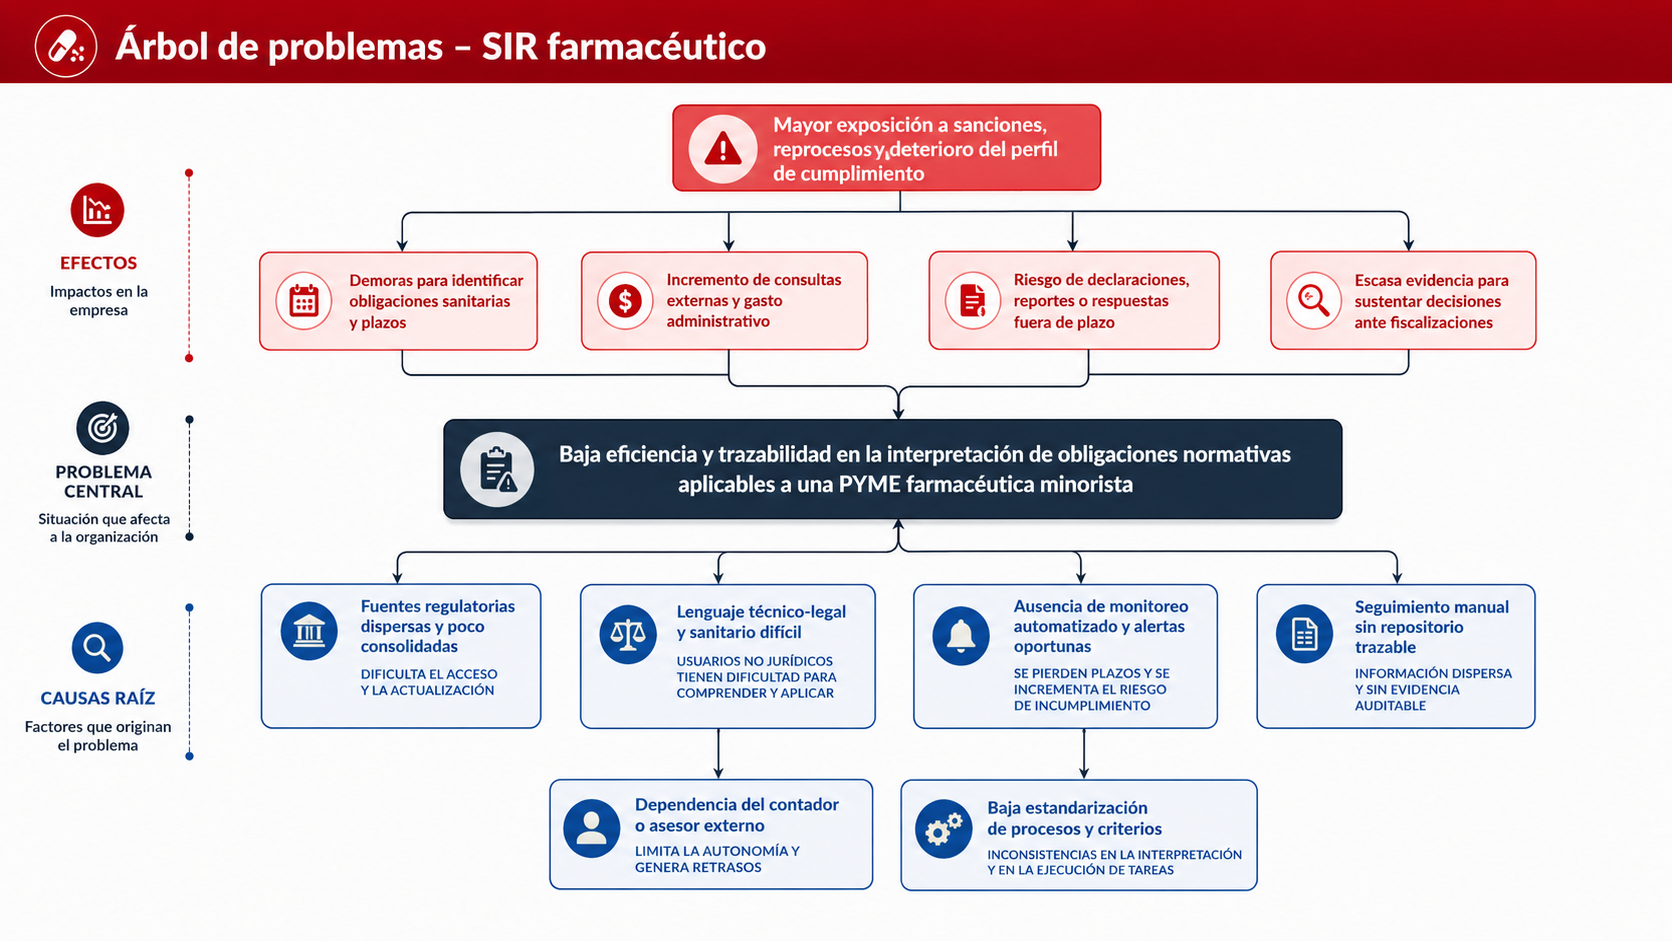
\includegraphics[width=6.5in,height=3.65625in]{figuras/docx_image4.png}

El árbol de problemas muestra que la farmacia presenta dificultades para
interpretar, organizar y dar seguimiento oportuno a sus obligaciones
normativas. Esta situación se origina por la dispersión de fuentes
regulatorias, el lenguaje técnico-legal y sanitario, la falta de alertas
automatizadas y el seguimiento manual sin repositorio trazable.

\textbf{Análisis del problema mediante Diagrama de Ishikawa:}

El Diagrama de Ishikawa de la Figura 3 complementa el Árbol de Problemas
al clasificar las causas en seis dimensiones: personas, métodos,
tecnología, información, normativa y gestión. Esta lectura permite
distinguir causas técnicas y causas de negocio, lo cual facilita
formular objetivos e indicadores de éxito coherentes con la solución
SIR.

\phantomsection\label{_Toc231672403}{}Figura 3\\
\emph{Diagrama de Ishikawa}

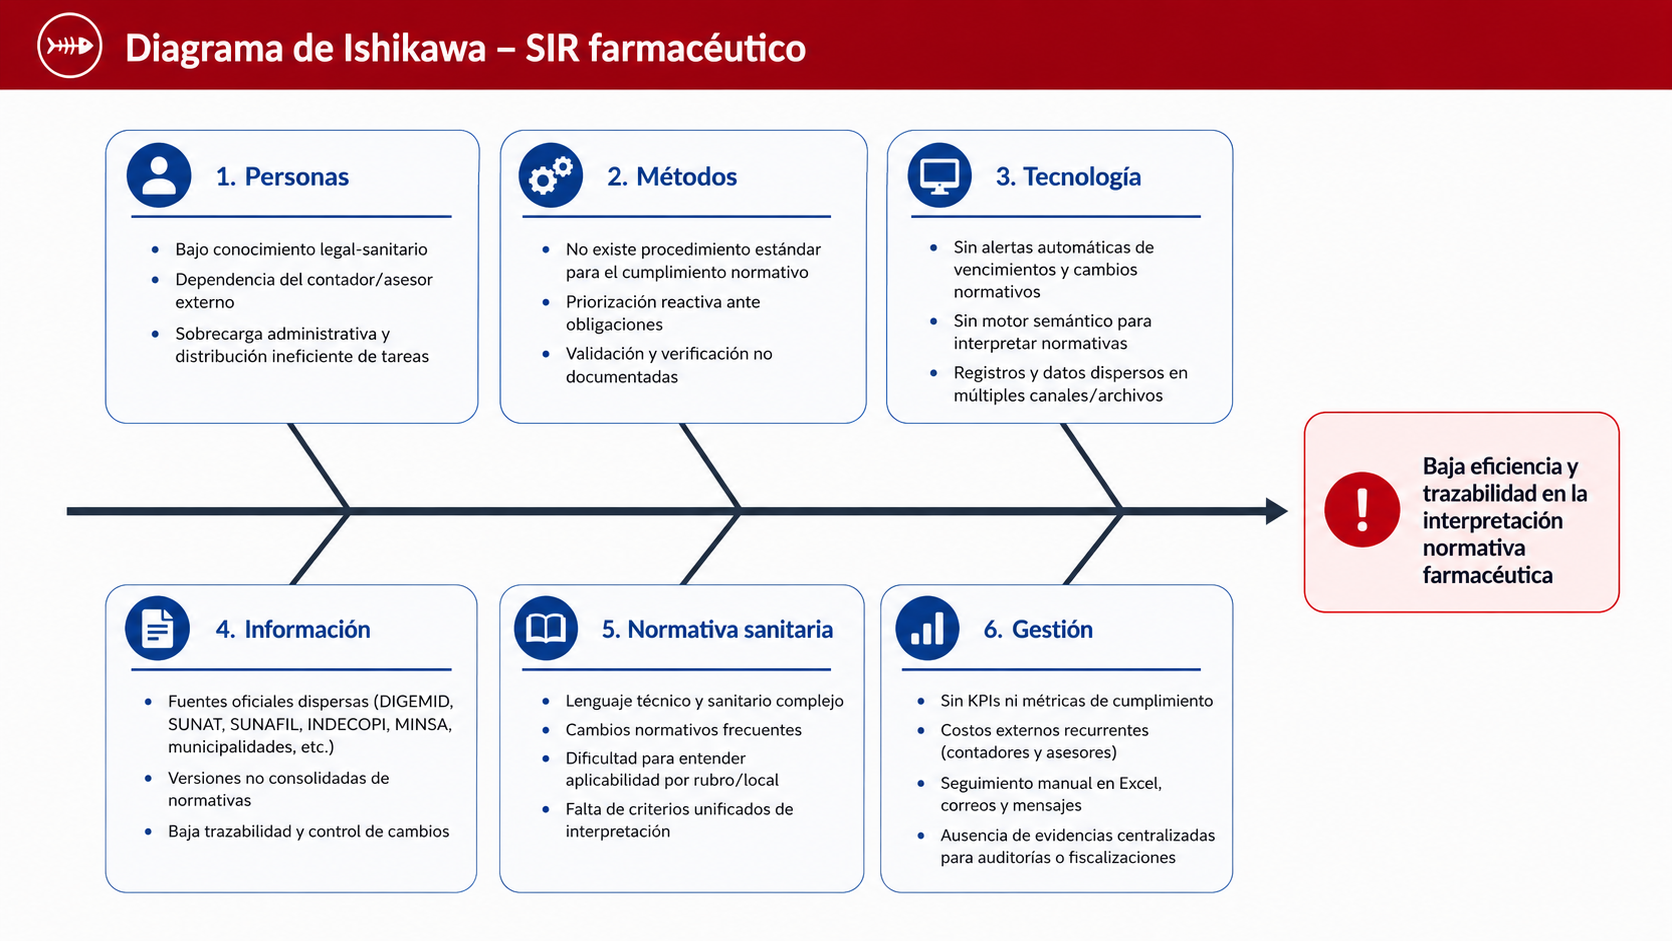
\includegraphics[width=6.5in,height=3.65625in]{figuras/docx_image5.png}

El diagrama de Ishikawa evidencia que la baja eficiencia y trazabilidad
en la interpretación normativa farmacéutica no depende de una sola
causa, sino de la combinación de factores relacionados con personas,
métodos, tecnología, información, normativa sanitaria y gestión. Entre
las principales causas se identifican la dependencia del contador o
asesor externo, la ausencia de procedimientos estandarizados, la falta
de alertas automáticas, las fuentes oficiales dispersas, el lenguaje
técnico-sanitario complejo y el seguimiento manual sin evidencias
centralizadas. Así, en conjunto, estas causas generan retrasos,
reprocesos, riesgo de incumplimiento y dificultad para sustentar
decisiones ante fiscalizaciones.

\subsubsection{1.1.4 Problemas a resolver}\label{problemas-a-resolver}

A partir del diagnóstico, los problemas a resolver se estructuran en
dimensiones técnicas y de negocio. Esta organización evita que la
problemática quede formulada de manera general y permite vincular cada
causa con una capacidad esperada del SIR. La Tabla 5 sintetiza el
problema central, sus causas principales y el enfoque de atención
propuesto.

\phantomsection\label{_Toc231672260}{}Tabla 5\\
\emph{Problemas a resolver según dimensión}

\begin{longtable}[]{@{}
  >{\raggedright\arraybackslash}p{(\columnwidth - 4\tabcolsep) * \real{0.2272}}
  >{\raggedright\arraybackslash}p{(\columnwidth - 4\tabcolsep) * \real{0.3785}}
  >{\raggedright\arraybackslash}p{(\columnwidth - 4\tabcolsep) * \real{0.3942}}@{}}
\toprule\noalign{}
\begin{minipage}[b]{\linewidth}\raggedright
Dimensión
\end{minipage} & \begin{minipage}[b]{\linewidth}\raggedright
Descripción del problema
\end{minipage} & \begin{minipage}[b]{\linewidth}\raggedright
Orientación de solución
\end{minipage} \\
\midrule\noalign{}
\endhead
\bottomrule\noalign{}
\endlastfoot
Problema central & Baja eficiencia y trazabilidad en la interpretación
de obligaciones normativas aplicables a una PYME farmacéutica minorista.
& Implementar un asistente de inteligencia regulatoria que responda
consultas con fuentes oficiales y orientación operativa. \\
Causas técnicas & Ausencia de monitoreo automatizado, búsqueda
semántica, repositorio centralizado y capa de citación verificable. &
Diseñar arquitectura RAG con ingesta normativa, recuperación vectorial,
generación controlada y citación de fuentes. \\
Causas de negocio & Dependencia del contador externo, desconocimiento
del lenguaje legal, seguimiento manual de plazos y poca claridad sobre
aplicabilidad por rubro. & Configurar perfil empresarial, alertas y
respuestas adaptadas al tamaño, rubro y obligaciones de la PYME. \\
Impactos medibles & Tiempo alto de interpretación, baja exactitud, bajo
registro de fuentes y costos recurrentes de asesoría. & Validar
reducción de tiempo, mejora de exactitud, cobertura de citaciones y
satisfacción del usuario. \\
\end{longtable}

\textbf{Formulación del problema:}

¿De qué manera la implementación de un Sistema de Inteligencia
Regulatoria basado en IA generativa y arquitectura RAG puede reducir el
tiempo de interpretación normativa y mejorar la trazabilidad de fuentes
en el proceso de cumplimiento de una PYME farmacéutica peruana?

\textbf{Problemas específicos:}

\begin{itemize}
\item
  La PYME no cuenta con un proceso centralizado para monitorear cambios
  normativos aplicables a su rubro, tamaño y ubicación.
\item
  La interpretación de normas tributarias, laborales y comerciales
  depende de personal sin formación jurídica o del contador externo.
\item
  Las fuentes oficiales usadas para tomar decisiones de cumplimiento no
  se registran de manera uniforme ni trazable.
\item
  Los plazos y acciones derivadas de cambios normativos se controlan
  manualmente, lo que genera riesgo de omisión o demora.
\item
  No existen indicadores internos para medir tiempo de interpretación,
  exactitud, cobertura de fuentes y satisfacción del usuario en el
  proceso de cumplimiento.
\end{itemize}

\subsection{1.2 Definición de la
Solución}\label{definiciuxf3n-de-la-soluciuxf3n}

La solución propuesta es el Sistema de Inteligencia Regulatoria (SIR),
una plataforma web de apoyo al cumplimiento normativo para PYMEs
farmacéuticas minoristas. El sistema integrará un perfil empresarial, un
motor de recuperación de normas oficiales, un asistente con- versacional
basado en IA generativa y una capa de citación que permita verificar la
procedencia de cada respuesta. La solución no reemplaza al contador ni
al asesor legal; su función es reducir la carga operativa de búsqueda e
interpretación preliminar, transformando normas complejas en respuestas
accionables, trazables y contextualizadas.

\subsubsection{1.2.1 Objetivos del
Proyecto}\label{objetivos-del-proyecto}

\textbf{Objetivo General:}

Implementar un Sistema de Inteligencia Regulatoria basado en IA
generativa y arquitectura RAG para automatizar la interpretación
preliminar de obligaciones normativas aplicables a una PYME farmacéutica
peruana, con el fin de reducir al menos en 60 \% el tiempo promedio de
comprensión normativa y alcanzar una cobertura de citaciones oficiales
de al menos 95 \% durante la validación del Sistema de Inteligencia
Regulatoria.

\textbf{Objetivos Específicos:}

\textbf{OE1:} Diagnosticar el proceso actual de identificación e
interpretación normativa de la PYME farmacéutica minorista,
estableciendo una línea base de tiempo, exactitud, dependencia externa y
trazabilidad de fuentes.

\textbf{OE2:} Diseñar la arquitectura lógica y funcional del SIR
mediante un enfoque RAG que integre ingesta normativa, almacenamiento
vectorial, recuperación semántica, generación de respuestas y citación
verificable.

\textbf{OE3:} Desarrollar el Sistema de Inteligencia Regulatoria (SIR)
que permita registrar el perfil empresarial, realizar consultas en
lenguaje natural, generar respuestas contextualizadas y mostrar fuentes
oficiales vinculadas.

\textbf{OE4:} Validar el desempeño técnico, operativo y de usabilidad
del Sistema de Inteligencia Regulatoria mediante métricas de precisión,
tiempo de respuesta, reducción del tiempo de interpretación, cobertura
de citaciones y satisfacción del usuario.

\subsubsection{1.2.2 Indicadores de
Éxito}\label{indicadores-de-uxe9xito}

Los indicadores de éxito se reformulan para asegurar correspondencia
directa con los objetivos específicos y con la problemática medible del
Capítulo 1. Cada indicador incluye fórmula, tipo de ratio, umbral de
aceptación y objetivo asociado.

\phantomsection\label{_Toc231672261}{}Tabla 6\\
\emph{Indicadores de éxito del proyecto}

\begin{longtable}[]{@{}
  >{\raggedright\arraybackslash}p{(\columnwidth - 10\tabcolsep) * \real{0.1503}}
  >{\raggedright\arraybackslash}p{(\columnwidth - 10\tabcolsep) * \real{0.2097}}
  >{\raggedright\arraybackslash}p{(\columnwidth - 10\tabcolsep) * \real{0.1755}}
  >{\raggedright\arraybackslash}p{(\columnwidth - 10\tabcolsep) * \real{0.1578}}
  >{\raggedright\arraybackslash}p{(\columnwidth - 10\tabcolsep) * \real{0.1520}}
  >{\raggedright\arraybackslash}p{(\columnwidth - 10\tabcolsep) * \real{0.1546}}@{}}
\toprule\noalign{}
\begin{minipage}[b]{\linewidth}\raggedright
Código
\end{minipage} & \begin{minipage}[b]{\linewidth}\raggedright
Descripción
\end{minipage} & \begin{minipage}[b]{\linewidth}\raggedright
Fórmula
\end{minipage} & \begin{minipage}[b]{\linewidth}\raggedright
Ratio
\end{minipage} & \begin{minipage}[b]{\linewidth}\raggedright
Umbral
\end{minipage} & \begin{minipage}[b]{\linewidth}\raggedright
Objetivo
\end{minipage} \\
\midrule\noalign{}
\endhead
\bottomrule\noalign{}
\endlastfoot
IE1 & Línea base documentada del proceso AS-IS. & Casos. diagnosticados
/ casos planificados. & Porcentaje & 100\% & OE1 \\
IE2 & Reducción del tiempo de interpretación normativa. & (Tiempo base -
tiempo con SIR) / tiempo base & Porcentaje & ≥ 60\% & OE4 \\
IE3 & Precisión de recuperación e interpretación. & F1-Score sobre
dataset etiquetado. & Índice & ≥ 0.85 & OE4 \\
IE4 & Cobertura de citaciones oficiales. & Respuestas con fuente oficial
/ total de respuestas. & Porcentaje & ≥ 95\% & OE2 \\
IE5 & Tiempo promedio de respuesta del chatbot. & Suma de tiempos de
respuesta / total de consultas. & Segundos & \textless{} 8s & OE4 \\
IE6 & Usabilidad percibida. & Puntuación System Usability Scale. &
Puntaje & ≥ 75 & OE4 \\
IE7 & Contextualización por perfil empresarial. & Respuestas que
consideran rubro/tamaño / total de respuestas aplicables. & Porcentaje &
≥ 90\% & OE3 \\
IE8 & Disponibilidad del Sistema de Inteligencia Regulatoria en ambiente
de validación. & Tiempo operativo / tiempo total planificado. &
Porcentaje & ≥ 99\% & OE3 \\
\end{longtable}

\subsubsection{1.2.3 Factibilidad del
Proyecto}\label{factibilidad-del-proyecto}

La factibilidad del proyecto se analiza considerando las dimensiones
económica y técnica, debido a que el Sistema de Inteligencia Regulatoria
debe ser implementado, desplegado y validado con usuarios finales en un
ambiente controlado. Este análisis permite determinar si la solución
puede ejecutarse con los recursos disponibles, qué dificultades podrían
presentarse y bajo qué condiciones puede operar de manera sostenible. En
esa línea, la evaluación económica se orienta a la relación
costo-beneficio, mientras que la evaluación técnica revisa si existen
conocimientos, herramientas e infraestructura suficientes para
desarrollar la solución.

\paragraph{1.2.3.1 Factibilidad
Económica}\label{factibilidad-econuxf3mica}

La factibilidad económica estima los costos necesarios para construir,
desplegar y validar el SIR en Inversiones y Representaciones Peruanas LK
S.R.L. (Boticas Farmaperu). Este análisis permite evaluar si conviene
ejecutar el proyecto a partir de criterios cuantitativos y cualitativos
como VAN, TIR, periodo de recuperación y relación costo-beneficio. Para
este proyecto, los costos se dividen en recursos humanos,
infraestructura cloud, software/licencias, hardware y otros gastos
operativos.

\textbf{Mapeo de costos involucrados:}

\phantomsection\label{_Toc231672262}{}Tabla 7\\
\emph{Mapeo de costos de inversión inicial}

\begin{longtable}[]{@{}
  >{\raggedright\arraybackslash}p{(\columnwidth - 4\tabcolsep) * \real{0.2771}}
  >{\raggedright\arraybackslash}p{(\columnwidth - 4\tabcolsep) * \real{0.4747}}
  >{\raggedright\arraybackslash}p{(\columnwidth - 4\tabcolsep) * \real{0.2482}}@{}}
\toprule\noalign{}
\begin{minipage}[b]{\linewidth}\raggedright
Tipo
\end{minipage} & \begin{minipage}[b]{\linewidth}\raggedright
Detalle
\end{minipage} & \begin{minipage}[b]{\linewidth}\raggedright
Costo estimado
\end{minipage} \\
\midrule\noalign{}
\endhead
\bottomrule\noalign{}
\endlastfoot
Recursos humanos & Análisis, diseño, desarrollo, pruebas y documentación
del Sistema de Inteligencia Regulatoria por dos integrantes del equipo.
& S/ 12,000 \\
Infraestructura & Ambiente cloud ligero para API, base de datos,
almacenamiento y pruebas de despliegue. & S/ 1,200 \\
Software/licencias & Consumo inicial de API de IA, herramientas de
desarrollo, monitoreo y servicios de integración. & S/ 1,800 \\
Hardware & Uso de laptops del equipo y dispositivos de prueba. No se
requiere adquisición adicional. & S/ 0 \\
Otros & Validación con usuarios, documentación, contingencia y
materiales administrativos. & S/ 1,200 \\
Total inversión inicial & & S/ 16,200 \\
\end{longtable}

\emph{Nota}. Elaboración propia con valores estimados para el escenario
de validación.

\textbf{Beneficios esperados:}

Los beneficios económicos esperados provienen principalmente de la
reducción de horas administrativas dedicadas a búsqueda normativa,
disminución de consultas externas recurrentes, reducción de reprocesos y
mejora en la oportunidad de cumplimiento. La Tabla 8 presenta una
estimación anual conservadora.

\phantomsection\label{_Toc231672263}{}Tabla 8\\
\emph{Beneficios económicos esperados}

\begin{longtable}[]{@{}
  >{\raggedright\arraybackslash}p{(\columnwidth - 4\tabcolsep) * \real{0.3726}}
  >{\raggedright\arraybackslash}p{(\columnwidth - 4\tabcolsep) * \real{0.4418}}
  >{\raggedright\arraybackslash}p{(\columnwidth - 4\tabcolsep) * \real{0.1856}}@{}}
\toprule\noalign{}
\begin{minipage}[b]{\linewidth}\raggedright
Beneficio
\end{minipage} & \begin{minipage}[b]{\linewidth}\raggedright
Supuesto de cálculo
\end{minipage} & \begin{minipage}[b]{\linewidth}\raggedright
Ahorro anual
\end{minipage} \\
\midrule\noalign{}
\endhead
\bottomrule\noalign{}
\endlastfoot
Reducción de horas administrativas & Ahorro de 2 horas semanales a S/ 25
por hora durante 48 semanas. & S/ 2,400 \\
Reducción de consultas externas & Disminución de S/ 350 a S/ 150
mensuales en consultas adicionales. & S/ 2,400 \\
Menor reproceso documental & Reducción de correcciones, búsqueda de
fuentes y duplicidad documental. & S/ 1,800 \\
Prevención de contingencias menores & Menor exposición a pagos por
errores operativos y retrasos menores. & S/ 3,600 \\
Total beneficio anual estimado & & S/ 10,200 \\
\end{longtable}

\emph{Nota}. Elaboración propia con valores estimados para fines de
evaluación económica preliminar.

\subparagraph{Análisis financiero:}\label{anuxe1lisis-financiero}

Se proyecta un flujo de caja a tres años con una inversión inicial de S/
16,200, beneficios crecientes por adopción progresiva y costos
operativos anuales asociados al uso de servicios cloud, API de IA y
mantenimiento del Sistema de Inteligencia Regulatoria. Se utiliza una
tasa de descuento referencial de 12 \%.

\phantomsection\label{_Toc231672264}{}Tabla 9\\
\emph{Flujo de caja proyectado a tres años}

\begin{longtable}[]{@{}
  >{\raggedright\arraybackslash}p{(\columnwidth - 6\tabcolsep) * \real{0.2206}}
  >{\raggedright\arraybackslash}p{(\columnwidth - 6\tabcolsep) * \real{0.3804}}
  >{\raggedright\arraybackslash}p{(\columnwidth - 6\tabcolsep) * \real{0.2000}}
  >{\raggedright\arraybackslash}p{(\columnwidth - 6\tabcolsep) * \real{0.1989}}@{}}
\toprule\noalign{}
\begin{minipage}[b]{\linewidth}\raggedright
Periodo
\end{minipage} & \begin{minipage}[b]{\linewidth}\raggedright
Beneficios
\end{minipage} & \begin{minipage}[b]{\linewidth}\raggedright
Costos operativos
\end{minipage} & \begin{minipage}[b]{\linewidth}\raggedright
Flujo neto
\end{minipage} \\
\midrule\noalign{}
\endhead
\bottomrule\noalign{}
\endlastfoot
Año 0 & S/ 0 & S/ 16,200 & -S/ 16,200 \\
Año 1 & S/ 10,200 & S/ 3,200 & S/ 7,000 \\
Año 2 & S/ 11,016 & S/ 3,426 & S/ 7,590 \\
Año 3 & S/ 11,897 & S/ 3,667 & S/ 8,230 \\
\end{longtable}

\phantomsection\label{_Toc231672265}{}Tabla 10\\
\emph{Indicadores financieros preliminares}

\begin{longtable}[]{@{}
  >{\raggedright\arraybackslash}p{(\columnwidth - 4\tabcolsep) * \real{0.3715}}
  >{\raggedright\arraybackslash}p{(\columnwidth - 4\tabcolsep) * \real{0.1827}}
  >{\raggedright\arraybackslash}p{(\columnwidth - 4\tabcolsep) * \real{0.4458}}@{}}
\toprule\noalign{}
\begin{minipage}[b]{\linewidth}\raggedright
Indicador
\end{minipage} & \begin{minipage}[b]{\linewidth}\raggedright
Resultado
\end{minipage} & \begin{minipage}[b]{\linewidth}\raggedright
Interpretación
\end{minipage} \\
\midrule\noalign{}
\endhead
\bottomrule\noalign{}
\endlastfoot
Valor Actual Neto (VAN) & S/ 1,959 & Al ser positivo, indica que el
proyecto genera valor bajo los supuestos estimados. \\
Tasa Interna de Retorno (TIR) & 18.7\% & Supera la tasa de descuento
referencial de 12 \%, por lo que el proyecto es atractivo. \\
Periodo de recuperación & Entre el año 2 y 3 & La inversión se recupera
dentro del horizonte de evaluación. \\
Relación beneficio/costo & 1.08 & Por cada sol invertido se obtiene un
retorno estimado de S/ 1.08. \\
\end{longtable}

\emph{Nota}. Cálculo preliminar con tasa de descuento de 12 \%.

Con base en los resultados, el proyecto es económicamente viable para
Inversiones y Representaciones Peruanas LK S.R.L. (Boticas Farmaperu) en
una etapa inicial de validación controlada. El VAN positivo, la TIR
superior a la tasa de descuento y la recuperación dentro del horizonte
de tres años indican que la inversión estimada se justifica por la
reducción de carga administrativa, consultas externas y reprocesos
asociados al cumplimiento normativo.

\paragraph{1.2.3.2 Factibilidad Técnica}\label{factibilidad-tuxe9cnica}

La factibilidad técnica evalúa si el equipo dispone de conocimientos,
herramientas, infraestructura y metodología suficientes para construir
el SIR. En este caso, la solución es técnicamente viable porque se basa
en tecnologías maduras y ampliamente documentadas: Python, FastAPI,
React, LangChain, modelos de lenguaje, embeddings y bases vectoriales.

\phantomsection\label{_Toc231672266}{}Tabla 11\\
\emph{Evaluación de factibilidad técnica}

\begin{longtable}[]{@{}
  >{\raggedright\arraybackslash}p{(\columnwidth - 2\tabcolsep) * \real{0.3624}}
  >{\raggedright\arraybackslash}p{(\columnwidth - 2\tabcolsep) * \real{0.6376}}@{}}
\toprule\noalign{}
\begin{minipage}[b]{\linewidth}\raggedright
Tipo
\end{minipage} & \begin{minipage}[b]{\linewidth}\raggedright
Detalles
\end{minipage} \\
\midrule\noalign{}
\endhead
\bottomrule\noalign{}
\endlastfoot
Infraestructura disponible & Despliegue cloud ligero para API, base de
datos relacional, almacenamiento documental y base vectorial. Se
priorizan servicios serverless o free-tier durante la validación. \\
Software y herramientas & Python, FastAPI, React, TypeScript, LangChain,
OpenAI API, Pinecone o Qdrant, PostgreSQL, GitHub, Docker y herramientas
de monitoreo básico. \\
Metodología tecnológica & Arquitectura RAG con ingesta, limpieza,
segmentación, embeddings, recuperación Top-K, generación controlada y
capa de citación. Desarrollo iterativo bajo Scrum. \\
Alternativas evaluadas & Pinecone frente a Qdrant para base vectorial;
OpenAI frente a modelos open-source; Vercel frente a despliegue cloud
tradicional. Se prioriza menor complejidad operativa. \\
Riesgos y limitaciones técnicas & Dependencia de API externa, costos
variables por consumo, límites de contexto del modelo, necesidad de
curar fuentes oficiales y riesgo de alucinaciones mitigado mediante
citaciones y respuestas con disclaimer. \\
\end{longtable}

El proyecto es técnicamente viable porque el equipo cuenta con
conocimientos de desarrollo web, Python, integración de APIs, bases de
datos y arquitectura de software. Asimismo, el alcance se limita al
Sistema de Inteligencia Regulatoria validable en Inversiones y
Representaciones Peruanas LK S.R.L. (Boticas Farmaperu), lo que reduce
la complejidad de despliegue y permite concentrar la evaluación en la
reducción de tiempo, trazabilidad y usabilidad.

\subsubsection{1.2.4 Propuesta preliminar de la
solución}\label{propuesta-preliminar-de-la-soluciuxf3n}

La propuesta preliminar del SIR se plantea como un proceso TO-BE de
apoyo al cumplimiento normativo. En lugar de que la PYME revise
manualmente múltiples portales y dependa del contador externo para
interpretar cada cambio, el sistema centraliza la consulta normativa,
recupera fuentes oficiales, genera una respuesta operativa y muestra la
evidencia que sustenta la recomendación. Esta propuesta mantiene al
usuario humano como responsable de la decisión final y al contador o
asesor como validador en casos de alta complejidad.

Alcance funcional de alto nivel:

\begin{itemize}
\item
  Registro del perfil empresarial: rubro, tamaño, ubicación, régimen
  tributario, número de trabajadores y canales de venta.
\item
  Ingesta y consulta de normas oficiales provenientes del Diario Oficial
  El Peruano y entidades regulatorias relevantes.
\item
  Chatbot de consultas en lenguaje natural para preguntas sanitarias,
  tributarias, laborales, municipales y de protección al consumidor.
\item
  Respuestas contextualizadas según perfil de la PYME, con resumen
  operativo, nivel de aplicabilidad y fuente oficial citada.
\item
  Alertas de cambios normativos relevantes y recordatorios de
  obligaciones recurrentes.
\item
  Exportación de respuestas y evidencias para revisión del contador o
  asesor externo.
\end{itemize}

Proceso TO-BE propuesto:

La Figura 4 presenta el flujo conceptual de la solución propuesta. Este
flujo no representa aún la arquitectura técnica detallada, sino la
manera en que el SIR apoyará el proceso de negocio de la PYME

\phantomsection\label{_Toc231672404}{}Figura 4\\
\emph{Proceso TO-BE de cumplimiento normativo asistido por SIR}

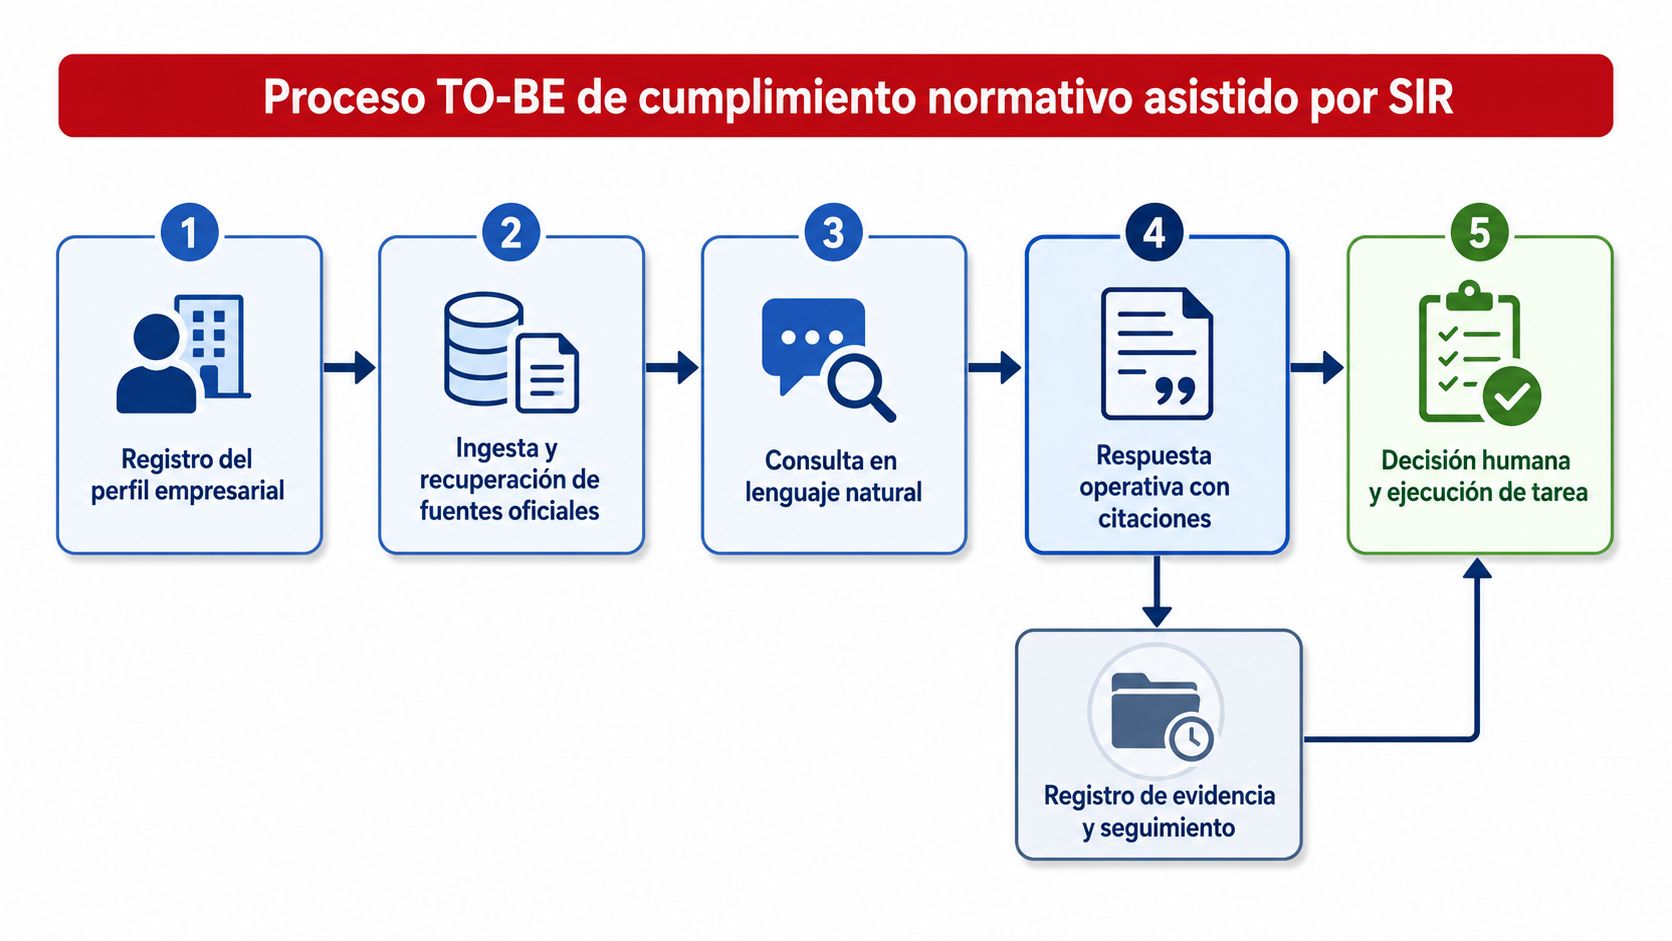
\includegraphics[width=6.5064in,height=3.02965in]{figuras/docx_image6.png}

En síntesis, el Capítulo 1 define un escenario medible y validable:
Inversiones y Representaciones Peruanas LK S.R.L. (Boticas Farmaperu),
una PYME farmacéutica minorista que necesita reducir la carga de
interpretación normativa. Esta definición mejora la coherencia entre
problemática, objeto de estudio, indicadores, factibilidad y solución
propuesta, y permite que los capítulos siguientes desarrollen la
arquitectura, implementación y validación del SIR con mayor precisión.

\section{2. Capítulo 2: Marco
Teórico}\label{capuxedtulo-2-marco-teuxf3rico}

El presente capítulo desarrolla los fundamentos teóricos que sustentan
la propuesta de solución basada en Inteligencia Artificial Generativa
con arquitectura Retrieval-Augmented Generation (RAG) aplicada a la
interpretación de normas legales para una PYME comercial peruana. A
partir de la revisión sistemática de literatura especializada y de
marcos conceptuales actualizados, se establecen las bases académicas,
técnicas y normativas que permiten comprender la problemática del
cumplimiento normativo en las PYMEs y orientar el diseño del sistema
propuesto.

El capítulo se organiza en tres dimensiones complementarias. En la
primera parte, se presenta el marco teórico relacionado al negocio y a
los procesos, donde se describen los conceptos, modelos y prácticas
vinculadas con el cumplimiento normativo, la gestión de riesgo
regulatorio (GRC) y la transformación digital del Estado peruano. En la
segunda parte, se aborda el marco teórico de las tecnologías de
información, que incluye los fundamentos de Procesamiento de Lenguaje
Natural, modelos de lenguaje grandes (LLMs), la arquitectura RAG y las
métricas estándar para evaluar sistemas de IA en dominios legales.
Finalmente, se expone el cumplimiento normativo, destacando las leyes
peruanas y los estándares internacionales que orientan el diseño y
operación de soluciones RegTech responsables.

Este capítulo resulta esencial porque proporciona el sustento científico
y técnico que respalda la coherencia entre los objetivos del proyecto,
la solución propuesta y las metodologías adoptadas. Los hallazgos se
apoyan en una revisión sistemática de 24 artículos científicos indexados
en bases académicas como Scopus, IEEE Xplore, ACM Digital Library y
SpringerLink, con énfasis en los aportes de Singh et al. (2022), Raju et
al. (2025) y Noronha et al. (2025) como fuentes principales que
sustentan el enfoque conceptual, técnico y de validación del Sistema de
Inteligencia Regulatoria (SIR).

\subsection{2.1 Marco teórico relacionado al negocio y a los
procesos}\label{marco-teuxf3rico-relacionado-al-negocio-y-a-los-procesos}

La presente sección desarrolla los fundamentos conceptuales vinculados
con la operación y gestión del cumplimiento normativo en organizaciones
empresariales, con énfasis en el segmento PYME. Se abordan cinco bloques
temáticos: la definición y evolución del campo RegTech y SupTech; el
modelo Governance, Risk and Compliance (GRC) como articulador del
cumplimiento; la caracterización del segmento PYME peruano; los procesos
administrativos de cumplimiento tributario, laboral y sectorial; y las
experiencias internacionales de innovación regulatoria que sirven de
referencia.

\subsubsection{2.1.1 RegTech y SupTech: definición y
evolución}\label{regtech-y-suptech-definiciuxf3n-y-evoluciuxf3n}

El término RegTech, acuñado por la Financial Conduct Authority del Reino
Unido en 2015, designa al conjunto de tecnologías de información, datos,
inteligencia artificial, software, utilizadas por las organizaciones
para cumplir con regulaciones de manera más eficaz y eficiente (El
Khoury et al., 2025). Complementariamente, SupTech (Supervisory
Technology) describe el uso de tecnología por parte de las autoridades
regulatorias para la supervisión y aplicación de las normas, con casos
de uso que incluyen el seguimiento automatizado de cambios normativos,
el reporting estandarizado y la detección de fraude (Chao et al., 2022).

Desde su origen en el sector financiero, el campo RegTech ha
experimentado una expansión hacia otras industrias reguladas, incluyendo
el sector legal (LegalTech), el sector salud (HealthTech regulatorio) y
el tercer sector (CharityTech). Singh et al. (2022) demuestran que las
tecnologías de aprendizaje automático aplicadas al cumplimiento
normativo pueden transferirse de organizaciones financieras a
organizaciones con recursos limitados, como las entidades benéficas en
el Reino Unido, donde los autores proponen un "Machine-Executable
Compliance Toolkit" capaz de actualizar políticas internas y generar
alertas de manera autónoma frente a cambios normativos. Este marco
conceptual constituye la base teórica del presente proyecto, pues
evidencia que la automatización del cumplimiento no se limita a grandes
corporaciones y resulta aplicable al segmento PYME.

Charoenwong et al. (2024) y Liu et al. (2022) consolidan el estado del
arte del campo RegTech identificando cuatro generaciones tecnológicas:
(i) digitalización de reportes regulatorios (RegTech 1.0), (ii)
automatización de procesos estructurados (RegTech 2.0), (iii) analítica
predictiva basada en machine learning clásico (RegTech 3.0) y (iv)
sistemas interpretativos basados en inteligencia artificial generativa y
grandes modelos de lenguaje (RegTech 4.0). El proyecto se posiciona en
la cuarta generación, que es la frontera actual del campo.

\subsubsection{2.1.2 Modelo de Gobernanza, Riesgo y Cumplimiento
(GRC)}\label{modelo-de-gobernanza-riesgo-y-cumplimiento-grc}

El modelo GRC (Governance, Risk and Compliance), desarrollado por la
Open Compliance and Ethics Group (OCEG) en su Red Book 3.5, integra tres
capacidades organizacionales que tradicionalmente operaban en silos: el
gobierno corporativo, la gestión integral de riesgos y el cumplimiento
normativo. El modelo se fundamenta en el concepto de "principled
performance" o desempeño con integridad, es decir, alcanzar objetivos
organizacionales de manera consistente con la regulación aplicable, los
valores éticos y las expectativas de los stakeholders.

OCEG estructura el modelo en cuatro fases iterativas: Aprender (Learn),
donde la organización mapea regulaciones, riesgos y stakeholders;
Alinear (Align), donde se definen políticas, controles y
responsabilidades; Ejecutar (Perform), donde se implementan y monitorean
los controles; y Revisar (Review), donde se mide el desempeño y se
ajusta el modelo. En el contexto de las PYMEs, la operacionalización del
modelo GRC suele estar limitada por restricciones de presupuesto y
conocimiento, situación que abre la oportunidad para herramientas
tecnológicas que automaticen las fases de Aprender y Ejecutar, como
propone el SIR.

Complementariamente, las normas internacionales ISO 37301:2021 (Sistemas
de Gestión de Cumplimiento) e ISO 31000:2018 (Gestión de Riesgos)
proveen marcos certificables para diseñar, implementar y mejorar
sistemas de cumplimiento y gestión de riesgos respectivamente. ISO 37301
establece requisitos sobre liderazgo, identificación de obligaciones,
evaluación de riesgos de cumplimiento, controles, auditoría y mejora
continua. ISO 31000 aporta principios y procesos genéricos para
identificar, analizar, tratar y monitorear riesgos, aplicables tanto al
riesgo regulatorio como al riesgo de uso de inteligencia artificial en
el sistema.

\subsubsection{2.1.3 Caracterización del segmento PYME
peruano}\label{caracterizaciuxf3n-del-segmento-pyme-peruano}

Las pequeñas y medianas empresas constituyen el núcleo del tejido
productivo peruano. De acuerdo con el Ministerio de la Producción
(PRODUCE, 2022), existen 3.5 millones de PYMEs formales activas en el
país, de las cuales el 95.6\% son microempresas, el 3.8\% son pequeñas
empresas y solo el 0.1\% son medianas. En conjunto generan más de 8.3
millones de empleos (48.3\% de la población económicamente activa y 91\%
del empleo del sector privado). La distribución sectorial muestra que el
49\% se ubica en servicios, el 33\% en comercio y el 15\% en actividades
productivas (INEI, 2024).

El presente proyecto se enfoca en una PYME del subsector comercio
especializado en farmacia, específicamente una botica minorista, acogida
al Régimen MYPE Tributario. El régimen MYPE, regulado por el Decreto
Legislativo N.º 1269 y modificatorias, está dirigido a contribuyentes
con ingresos netos anuales no superiores a 1,700 UIT y otorga beneficios
tributarios específicos como tasas reducidas y plazos diferenciados. La
selección de una PYME farmacéutica se justifica porque concentra una
doble carga regulatoria: las obligaciones generales del subsector
comercio (SUNAT, SUNAFIL, INDECOPI, municipalidad) y las obligaciones
sectoriales sanitarias propias de los establecimientos farmacéuticos
(DIGEMID/MINSA). Esta dualidad permite construir un escenario de
validación de mayor representatividad que un comercio común y dispone de
estadísticas públicas que permiten establecer una línea base medible
para el problema de investigación.

Según los reportes de la Cámara de Comercio de Lima (CCL, 2025) y Cruz
Rambaud y Expósito Gázquez (2022) en una investigación comparable
realizada en España, las PYMEs comerciales enfrentan una carga
regulatoria desproporcionada respecto de su tamaño y facturación. Los
autores españoles documentan que la implementación de soluciones RegTech
reduce significativamente los tiempos de cumplimiento y mitiga el riesgo
de sostenibilidad de las empresas pequeñas, hallazgo transferible al
contexto peruano por la similitud estructural del segmento.

\subsubsection{2.1.4 Procesos administrativos de cumplimiento
normativo}\label{procesos-administrativos-de-cumplimiento-normativo}

Una PYME comercial peruana debe atender, como mínimo, cuatro frentes de
cumplimiento normativo: el frente tributario (con SUNAT como ente
fiscalizador), el frente laboral (con SUNAFIL), el frente de protección
al consumidor (con INDECOPI) y el frente sectorial sanitario (con
DIGEMID/MINSA), al que se suman las obligaciones municipales (licencia
de funcionamiento, defensa civil y tributos). En el caso de una PYME
farmacéutica minorista como Boticas Farmaperu, el frente sanitario
adquiere especial relevancia por la regulación de la Ley N.º 29459 y el
Reglamento de Establecimientos Farmacéuticos. La siguiente tabla resume
los procesos típicos por frente.

\phantomsection\label{_Toc231672267}{}Tabla 12\\
\emph{Frentes de cumplimiento normativo de una PYME comercial}

\begin{longtable}[]{@{}
  >{\raggedright\arraybackslash}p{(\columnwidth - 6\tabcolsep) * \real{0.2500}}
  >{\raggedright\arraybackslash}p{(\columnwidth - 6\tabcolsep) * \real{0.2500}}
  >{\raggedright\arraybackslash}p{(\columnwidth - 6\tabcolsep) * \real{0.2500}}
  >{\raggedright\arraybackslash}p{(\columnwidth - 6\tabcolsep) * \real{0.2500}}@{}}
\toprule\noalign{}
\begin{minipage}[b]{\linewidth}\raggedright
Frente
\end{minipage} & \begin{minipage}[b]{\linewidth}\raggedright
Ente regulador
\end{minipage} & \begin{minipage}[b]{\linewidth}\raggedright
Proceso típico
\end{minipage} & \begin{minipage}[b]{\linewidth}\raggedright
Frecuencia
\end{minipage} \\
\midrule\noalign{}
\endhead
\bottomrule\noalign{}
\endlastfoot
Tributario & SUNAT & Declaración mensual (PDT 621), libros electrónicos,
comprobantes de pago, fiscalización & Mensual / Eventual \\
Laboral & SUNAFIL & Planilla electrónica, contratos, seguridad y salud,
fiscalización & Mensual / Eventual \\
Protección al consumidor & INDECOPI & Libro de reclamaciones,
etiquetado, publicidad, atención de denuncias & Continuo \\
Licencia y funcionamiento & Municipalidad distrital & Licencia de
funcionamiento, defensa civil, tributos municipales & Anual \\
Sanitario / sectorial & DIGESA, MINSA u otros & Permisos sanitarios y
certificaciones según rubro & Anual / Eventual \\
\end{longtable}

Cada uno de estos procesos genera obligaciones específicas que se
publican y modifican periódicamente en el Diario Oficial El Peruano. La
interpretación operativa de cada norma, es decir, responder a la
pregunta \textquotesingle¿qué tengo que hacer
concretamente?\textquotesingle, es la actividad cuyo costo cognitivo y
económico el SIR busca reducir. En el caso particular de las PYMEs
farmacéuticas como Boticas Farmaperu, además de los frentes señalados,
se añade un cuarto frente sectorial de alta densidad regulatoria: la
regulación sanitaria especializada bajo competencia de DIGEMID y MINSA.
Este marco está dado principalmente por la Ley N.º 29459 (Ley de los
Productos Farmacéuticos, Dispositivos Médicos y Productos Sanitarios) y
su Reglamento de Establecimientos Farmacéuticos (D.S. 014-2011-SA y
modificatorias), normas que establecen requisitos de autorización
sanitaria, dirección técnica farmacéutica, Buenas Prácticas de
Almacenamiento y Dispensación, registro sanitario de productos, control
de medicamentos y fiscalización periódica. Para una PYME farmacéutica
minorista, este frente concentra la mayor frecuencia de modificatorias y
el lenguaje técnico-sanitario más complejo, motivo por el cual la
solución SIR debe incorporarlo dentro del corpus normativo y del flujo
de respuestas contextualizadas.

\subsubsection{2.1.5 Experiencias internacionales de innovación
regulatoria}\label{experiencias-internacionales-de-innovaciuxf3n-regulatoria}

Como referencia internacional, varios países han implementado
estrategias de innovación regulatoria que combinan automatización y
supervisión flexible. Estonia, con su plataforma X-Road implementada en
2001, interconecta más de 450 instituciones y 52,000 organizaciones,
generando ahorros equivalentes a más de 1,400 años de trabajo
administrativo anuales y consagrando el principio "once-only" (World
Economic Forum, 2017). Singapur ha impulsado el MAS RegTech Grant
Scheme, con una inversión de USD 42 millones para promover la
automatización en KYC y reportes regulatorios. El Reino Unido, a través
de la Financial Conduct Authority, creó en 2015 el primer sandbox
regulatorio formal, apoyando a más de 200 compañías en siete cohortes
(Charoenwong et al., 2024).

En América Latina, Colombia ha dado pasos notables en LegalTech mediante
la regulación de smart contracts y la automatización de servicios
notariales (Rincón Cárdenas y Martínez Molano, 2022), mientras que Chile
y México han creado sandboxes regulatorios financieros. El Perú, en
cambio, mantiene un ecosistema de innovación regulatoria incipiente, lo
cual abre una oportunidad estratégica para que iniciativas académicas
como el SIR contribuyan a cerrar la brecha mediante una solución
concreta orientada al segmento PYME.

\subsection{2.2 Marco teórico relacionado a las tecnologías de
información}\label{marco-teuxf3rico-relacionado-a-las-tecnologuxedas-de-informaciuxf3n}

La presente sección desarrolla los fundamentos tecnológicos que
sustentan la arquitectura del Sistema de Inteligencia Regulatoria. Se
abordan seis bloques: el Procesamiento de Lenguaje Natural (PLN)
aplicado al dominio legal; la evolución hacia los modelos de lenguaje
grandes (LLMs) y la inteligencia artificial generativa; la arquitectura
Retrieval-Augmented Generation (RAG); las técnicas de embeddings y bases
de datos vectoriales; las métricas y benchmarks de evaluación; y los
marcos arquitectónicos para el diseño de soluciones de software.

\subsubsection{2.2.1 Procesamiento de Lenguaje Natural en el dominio
legal}\label{procesamiento-de-lenguaje-natural-en-el-dominio-legal}

El Procesamiento de Lenguaje Natural (PLN o NLP por sus siglas en
inglés) es la rama de la inteligencia artificial que estudia la
interacción entre las computadoras y el lenguaje humano natural. En el
dominio legal, el PLN se aplica a tareas como clasificación de
documentos jurídicos, extracción de entidades (NER), por ejemplo,
identificar números de norma, fechas y obligacione, resumen automático y
respuesta a preguntas. Alcántara-Francia et al. (2024) demuestran la
viabilidad de modelos de clasificación interpretables aplicados a
resoluciones administrativas peruanas, evidenciando que el lenguaje
técnico-jurídico es modelable y procesable.

Históricamente, el PLN aplicado a textos legales ha evolucionado en tres
etapas: (i) métodos basados en reglas y diccionarios, propios de los
años 90; (ii) métodos estadísticos y de aprendizaje automático
tradicional, SVM, Random Forest, Naive Bayes, dominantes hasta mediados
de la década de 2010; y (iii) métodos basados en aprendizaje profundo y
redes neuronales tipo Transformer, que constituyen el estándar actual.
Noronha et al. (2025) sintetizan esta evolución y concluyen que los
modelos Transformer "superan a los métodos tradicionales por un amplio
margen" en tareas de clasificación, resumen y reconocimiento de
entidades en textos jurídicos.

\subsubsection{2.2.2 Modelos de Lenguaje Grandes (LLMs) e IA
Generativa}\label{modelos-de-lenguaje-grandes-llms-e-ia-generativa}

Los Modelos de Lenguaje Grandes (Large Language Models, LLMs) son
arquitecturas de redes neuronales profundas, generalmente basadas en la
familia Transformer (Vaswani et al., 2017), preentrenadas sobre corpus
masivos de texto. Su capacidad de generar lenguaje fluido, coherente y
contextualizado los ha convertido en la base tecnológica de la
denominada Inteligencia Artificial Generativa. Modelos como GPT-4
(OpenAI), Claude (Anthropic), Llama (Meta) y DeepSeek (DeepSeek AI)
representan el estado del arte actual.

En el dominio legal, modelos especializados como Legal-BERT (Chalkidis
et al., 2020) han demostrado que el preentrenamiento específico mejora
significativamente el desempeño en tareas jurídicas. Sin embargo, los
LLMs generales más recientes, particularmente cuando se combinan con
técnicas de recuperación de información, alcanzan resultados
competitivos sin requerir preentrenamiento específico, lo cual los
vuelve operativamente viables para proyectos con presupuesto limitado.

Raju et al. (2025), en su sistema LegalMind basado en DeepSeek,
documentan reducciones significativas de tiempo y costo en servicios
legales mediante el uso de IA agéntica sobre LLMs. Los autores concluyen
que el aporte principal de los LLMs en el dominio legal no radica
únicamente en su precisión técnica, sino en su capacidad de transformar
tareas cognitivas costosas en operaciones rutinarias accesibles a
usuarios no expertos. Este hallazgo es directamente aplicable al SIR,
donde los usuarios finales son dueños y administradores de PYMEs sin
formación jurídica.

\subsubsection{2.2.3 Arquitectura Retrieval-Augmented Generation
(RAG)}\label{arquitectura-retrieval-augmented-generation-rag}

La arquitectura Retrieval-Augmented Generation (RAG), originalmente
propuesta por Lewis et al. (2020), combina dos componentes: un módulo de
recuperación de información, que busca documentos relevantes en una base
de conocimiento indexada vectorialmente, y un módulo de generación, que
produce una respuesta en lenguaje natural condicionada por los
documentos recuperados. La integración de ambos permite respuestas
factuales, trazables y actualizadas sin necesidad de reentrenar el
modelo de lenguaje.

La elección de RAG como arquitectura central del SIR responde a tres
motivos fundamentados en la literatura. Primero, la trazabilidad: cada
respuesta generada puede asociarse a las fuentes específicas
recuperadas, lo cual es indispensable para el dominio legal donde la
verificabilidad es un requisito regulatorio. Segundo, la mitigación de
alucinaciones: al anclar el modelo a documentos reales, se reduce
drásticamente la generación de información inventada, problema reportado
por Siering (2022) como uno de los mayores riesgos del uso de IA en el
cumplimiento. Tercero, la actualización dinámica: el corpus normativo
cambia diariamente, y RAG permite incorporar nuevas normas sin
reentrenar el modelo.

\phantomsection\label{_Toc231672268}{}Tabla 13\\
\emph{Componentes de la arquitectura RAG del SIR}

\begin{longtable}[]{@{}
  >{\raggedright\arraybackslash}p{(\columnwidth - 4\tabcolsep) * \real{0.3262}}
  >{\raggedright\arraybackslash}p{(\columnwidth - 4\tabcolsep) * \real{0.3261}}
  >{\raggedright\arraybackslash}p{(\columnwidth - 4\tabcolsep) * \real{0.3478}}@{}}
\toprule\noalign{}
\begin{minipage}[b]{\linewidth}\raggedright
Componente RAG
\end{minipage} & \begin{minipage}[b]{\linewidth}\raggedright
Función
\end{minipage} & \begin{minipage}[b]{\linewidth}\raggedright
Tecnología elegida
\end{minipage} \\
\midrule\noalign{}
\endhead
\bottomrule\noalign{}
\endlastfoot
Cargador (Loader) & Extrae normas del Diario Oficial El Peruano (PDF y
HTML). & BeautifulSoup + PyMuPDF \\
Procesador (Splitter) & Segmenta los textos en chunks coherentes
preservando estructura legal. & LangChain
RecursiveCharacterTextSplitter \\
Codificador (Embedder) & Convierte chunks de texto en vectores
semánticos. & OpenAI text-embedding-3-large \\
Base vectorial (Vector Store) & Almacena y permite búsqueda por
similitud coseno. & Pinecone (free tier) \\
Recuperador (Retriever) & Recupera los k documentos más relevantes para
la consulta. & Pinecone Top-K + filtros por rubro/sector \\
Generador (LLM) & Produce la respuesta condicionada por los documentos
recuperados. & OpenAI GPT-4 + LangChain \\
Citador (Citation Layer) & Asocia cada afirmación a su fuente y la
presenta verificable. & Implementación propia sobre LangChain output
parsers \\
\end{longtable}

\subsubsection{2.2.4 Embeddings y bases de datos
vectoriales}\label{embeddings-y-bases-de-datos-vectoriales}

Los embeddings son representaciones vectoriales densas de palabras,
frases o documentos en un espacio semántico de alta dimensionalidad. Los
modelos modernos generan embeddings de 768 a 3072 dimensiones, donde la
similitud entre vectores, medida típicamente por similitud coseno,
refleja la similitud semántica entre los textos correspondientes. Esto
permite que una consulta del usuario, codificada como vector, recupere
fragmentos normativos semánticamente relacionados aunque no compartan
palabras exactas.

Las bases de datos vectoriales, como Pinecone, Qdrant, Milvus o
Weaviate, están optimizadas para almacenar y consultar grandes
colecciones de embeddings con baja latencia. Para el SIR se selecciona
Pinecone por su plan gratuito de hasta 100,000 vectores, su modelo
serverless que evita la administración de infraestructura y su
integración nativa con LangChain. Con un tamaño promedio estimado de 500
tokens por chunk y un volumen esperado de 30,000 normas indexadas en el
primer año, se ocuparán aproximadamente 60,000 vectores, dentro del
límite gratuito.

\subsubsection{2.2.5 Métricas y benchmarks de
evaluación}\label{muxe9tricas-y-benchmarks-de-evaluaciuxf3n}

La evaluación de sistemas de IA en dominios legales requiere un enfoque
multidimensional. La revisión de literatura identifica cuatro familias
de métricas relevantes para el SIR.

\paragraph{2.2.5.1 Métricas de
clasificación}\label{muxe9tricas-de-clasificaciuxf3n}

Las métricas estándar para tareas de clasificación de documentos son
Accuracy, Precision, Recall y F1-Score. La métrica F1, media armónica de
Precision y Recall, es particularmente útil cuando las clases son
desbalanceadas, situación habitual en corpus normativos. Noronha et al.
(2025) y Orosz et al. (2021) reportan valores de F1 superiores a 0.85
como umbral de viabilidad industrial en tareas legales, métrica adoptada
como meta del proyecto (IE7).

\paragraph{2.2.5.2 Métricas de resumen y
generación}\label{muxe9tricas-de-resumen-y-generaciuxf3n}

Las métricas ROUGE (Lin, 2004) y BLEU (Papineni et al., 2002) evalúan
resúmenes y traducciones automáticas comparando los n-gramas generados
con un "gold standard" humano. Aunque son ampliamente usadas, presentan
limitaciones reconocidas para evaluar la calidad semántica genuina, por
lo que se complementan con evaluación humana experta.

\paragraph{2.2.5.3 Métricas de validación humana (Human vs
Machine)}\label{muxe9tricas-de-validaciuxf3n-humana-human-vs-machine}

Orosz et al. (2021), en un estudio LegalTech con paralegales y ML,
reportan que la tasa de error humano en interpretación legal puede
reducirse del 9.24\% al 2.6\% con apoyo de herramientas automatizadas,
evidencia clave para sustentar el indicador de reducción de error humano
del SIR.

\paragraph{2.2.5.4 Métricas de usabilidad: System Usability Scale
(SUS)}\label{muxe9tricas-de-usabilidad-system-usability-scale-sus}

El SUS es un cuestionario estandarizado de 10 preguntas con escala
Likert que produce una puntuación de 0 a 100. Una puntuación SUS ≥ 75 se
considera "buena" en la literatura de interacción humano-computadora.
Para el SIR se define un umbral de SUS ≥ 75 (IE9), aplicable al cierre
del Sprint 4 con usuarios reales de la PYME piloto.

\paragraph{2.2.5.5 Métricas operativas y de
negocio}\label{muxe9tricas-operativas-y-de-negocio}

Raju et al. (2025), en su sistema LegalMind, proponen un marco de
validación multidimensional con cuatro pilares: Exactitud técnica,
Impacto en tiempo y costo, Riesgo (tasa de error frente a humano) y
Complejidad percibida. Este marco se adopta como referencia para el
Marco de Validación Integral (MVI) del SIR, descrito en el Capítulo 5.

\subsubsection{2.2.6 Marcos arquitectónicos para el diseño de
software}\label{marcos-arquitectuxf3nicos-para-el-diseuxf1o-de-software}

El diseño de la arquitectura del SIR se apoya en dos marcos
complementarios. Primero, el modelo C4 (Context, Container, Component,
Code) propuesto por Simon Brown, que provee niveles progresivos de
abstracción para documentar arquitecturas de software. Segundo, el
modelo 4+1 de Kruchten (1995), que describe la arquitectura desde cinco
vistas complementarias: lógica, de procesos, de despliegue, de
implementación y de escenarios.

Adicionalmente, los atributos de calidad del software se operacionalizan
siguiendo el estándar ISO/IEC 25010, que identifica ocho
características, adecuación funcional, eficiencia de desempeño,
compatibilidad, usabilidad, fiabilidad, seguridad, mantenibilidad y
portabilidad, y se documentan los "drivers" arquitectónicos según la
metodología de Bass, Clements y Kazman en "Software Architecture in
Practice". Los detalles de la arquitectura se desarrollan en el Capítulo
3 del presente documento.

\subsection{2.3 Marco teórico relacionado al cumplimiento
normativo}\label{marco-teuxf3rico-relacionado-al-cumplimiento-normativo}

La presente sección expone el marco normativo aplicable al diseño y
operación del Sistema de Inteligencia Regulatoria. Se abordan tres
bloques: el marco normativo peruano que regula tanto la actividad de la
PYME piloto como el procesamiento de datos personales, la propiedad
intelectual y los servicios digitales; los estándares internacionales de
IA responsable; y las consideraciones éticas para el despliegue de
sistemas generativos en dominios sensibles.

\subsubsection{2.3.1 Marco normativo peruano aplicable al
proyecto}\label{marco-normativo-peruano-aplicable-al-proyecto}

El proyecto se desarrolla bajo el marco normativo peruano vigente, cuyo
cumplimiento es condición necesaria tanto para el despliegue del sistema
como para su operación con la PYME piloto. La siguiente tabla resume las
principales normas aplicables.

\phantomsection\label{_Toc231672269}{}Tabla 14\\
\emph{Marco normativo peruano aplicable al SIR}

\begin{longtable}[]{@{}
  >{\raggedright\arraybackslash}p{(\columnwidth - 4\tabcolsep) * \real{0.3333}}
  >{\raggedright\arraybackslash}p{(\columnwidth - 4\tabcolsep) * \real{0.3333}}
  >{\raggedright\arraybackslash}p{(\columnwidth - 4\tabcolsep) * \real{0.3333}}@{}}
\toprule\noalign{}
\begin{minipage}[b]{\linewidth}\raggedright
Norma
\end{minipage} & \begin{minipage}[b]{\linewidth}\raggedright
Materia
\end{minipage} & \begin{minipage}[b]{\linewidth}\raggedright
Aplicación al SIR
\end{minipage} \\
\midrule\noalign{}
\endhead
\bottomrule\noalign{}
\endlastfoot
Ley N.º 29733 y su Reglamento (D.S. 003-2024-JUS) & Protección de datos
personales & El SIR procesa RUC, datos de empresa y consultas; debe
aplicar minimización, finalidad y consentimiento explícito. \\
D. Leg. N.º 1412 (Ley de Gobierno Digital) y reglamento & Servicios
digitales e identidad digital & Marco habilitador del intercambio
digital con entidades públicas (PIDE). \\
Ley N.º 27269 (Firmas y certificados digitales) & Equivalencia jurídica
de firma digital & Permite garantizar integridad y autenticidad de
documentos normativos consumidos. \\
Ley N.º 27806 (Transparencia y acceso a la información pública) & Acceso
a normas y actos públicos & Habilita el consumo y reutilización del
contenido del Diario Oficial El Peruano. \\
Ley N.º 31814 (Promoción del uso de IA en el Perú) & Inteligencia
Artificial & Fundamento legal del uso de IA basada en principios éticos
y de transparencia. \\
D. Leg. N.º 1269 y modificatorias (Régimen MYPE Tributario) & Régimen
tributario de la PYME piloto & Define obligaciones tributarias
específicas de la organización objeto de estudio. \\
Decreto de Urgencia N.º 007-2020 (Marco de confianza digital) &
Confianza digital y seguridad de la información & Aplicable a operación
del sistema y manejo de incidentes. \\
\end{longtable}

Sarabdeen (2023) ofrece evidencia comparable para Arabia Saudita, donde
el autor analiza la adecuación del marco legal para soluciones RegTech y
concluye que la robustez normativa es una condición necesaria pero no
suficiente para la adopción tecnológica. McCarthy (2023) profundiza en
las condiciones de consistencia regulatoria entre RegTech y SupTech,
hallazgos que orientan el diseño del SIR para que sea coherente con la
supervisión peruana.

\subsubsection{2.3.2 Estándares internacionales de IA
responsable}\label{estuxe1ndares-internacionales-de-ia-responsable}

El despliegue de sistemas de inteligencia artificial debe alinearse con
marcos internacionales de IA responsable. Tres marcos son
particularmente relevantes para el SIR.

\phantomsection\label{_Toc231672270}{}Tabla 15\\
\emph{Marcos internacionales de IA responsable}

\begin{longtable}[]{@{}
  >{\raggedright\arraybackslash}p{(\columnwidth - 4\tabcolsep) * \real{0.3333}}
  >{\raggedright\arraybackslash}p{(\columnwidth - 4\tabcolsep) * \real{0.3333}}
  >{\raggedright\arraybackslash}p{(\columnwidth - 4\tabcolsep) * \real{0.3333}}@{}}
\toprule\noalign{}
\begin{minipage}[b]{\linewidth}\raggedright
Marco
\end{minipage} & \begin{minipage}[b]{\linewidth}\raggedright
Año
\end{minipage} & \begin{minipage}[b]{\linewidth}\raggedright
Aporte al SIR
\end{minipage} \\
\midrule\noalign{}
\endhead
\bottomrule\noalign{}
\endlastfoot
Principios de IA de la OCDE & 2019 (actualización 2024) & Cinco
principios: crecimiento inclusivo, valores centrados en lo humano,
transparencia, robustez y rendición de cuentas. Adoptados como base de
diseño. \\
NIST AI Risk Management Framework (AI RMF 1.0) & 2023 & Cuatro
funciones: Govern, Map, Measure, Manage. Provee la estructura para
gestionar riesgos de IA en el ciclo de vida del SIR. \\
UNESCO Recommendation on the Ethics of AI & 2021 & Marco de derechos
humanos y dignidad aplicable a sistemas que afectan a poblaciones
vulnerables (PYMEs sin asesoría legal). \\
\end{longtable}

La adopción de estos marcos no es retórica: cada principio se
operacionaliza en decisiones técnicas concretas. La transparencia se
materializa en la cobertura de citaciones (IE4 ≥ 95\%); la rendición de
cuentas, en la trazabilidad completa de cada respuesta; la robustez, en
los umbrales de F1-Score (IE7 ≥ 0.85) y latencia (IE8 \textless{} 8s); y
los valores centrados en lo humano, en la métrica SUS (IE9 ≥ 75).

\subsubsection{2.3.3 Consideraciones éticas en el
despliegue}\label{consideraciones-uxe9ticas-en-el-despliegue}

Siering (2022), en su análisis de explicabilidad y equidad de soluciones
RegTech, identifica tres riesgos éticos centrales: (i) la opacidad
algorítmica ("caja negra"), que se mitiga con la trazabilidad RAG; (ii)
los sesgos en los datos de entrenamiento, abordados mediante curación
del corpus normativo; y (iii) la sustitución indebida del juicio humano
experto, mitigada con un disclaimer legal explícito que indica que el
SIR es una herramienta de apoyo y no sustituye el asesoramiento
profesional vinculante.

Adicionalmente, Eluwole y Akande (2022) advierten sobre los riesgos de
sobreconfianza del usuario en sistemas de IA, particularmente en
finanzas. La respuesta de diseño del SIR es exhibir siempre las fuentes
y el grado de confianza de la respuesta, y permitir al usuario solicitar
la opinión humana cuando el sistema reporte incertidumbre.

\subsection{2.4 Conclusiones}\label{conclusiones}

El presente capítulo ha desarrollado los fundamentos teóricos que
sustentan la propuesta del Sistema de Inteligencia Regulatoria. A partir
de la revisión sistemática de 24 artículos científicos y de marcos
conceptuales internacionales, se concluye lo siguiente.

Primero, en el plano de negocio y procesos, queda demostrado que el
cumplimiento normativo en las PYMEs peruanas es un problema estructural,
cuantificado por reportes oficiales del Banco Mundial, INEI y PRODUCE, y
que la transferencia de tecnologías RegTech desde sectores intensivos en
regulación (financiero, charities, legal) hacia el segmento PYME es
viable conceptualmente, como sustenta el marco "Machine-Executable
Compliance Toolkit" propuesto por Singh et al. (2022) y validado en
mercados emergentes por Sarabdeen (2023) y Cruz Rambaud y Expósito
Gázquez (2022). Esta conclusión justifica la pertinencia del proyecto.

Segundo, en el plano tecnológico, la literatura es concluyente respecto
a la superioridad de los modelos Transformer y la arquitectura
Retrieval-Augmented Generation (RAG) frente a las técnicas tradicionales
de aprendizaje automático para tareas legales. Noronha et al. (2025)
documentan que los modelos basados en LLMs superan por amplio margen a
los métodos clásicos en clasificación, NER y resumen, alcanzando
F1-Score superiores al 85\% en benchmarks estándar. La selección técnica
del SIR (RAG con GPT-4 + Pinecone + LangChain) está, por tanto, alineada
con el estado del arte y operacionalmente viable bajo restricciones
académicas. Esta conclusión justifica la decisión arquitectónica del
proyecto.

Tercero, en el plano de validación, el marco multidimensional propuesto
por Raju et al. (2025) en su sistema LegalMind, que integra exactitud
técnica, impacto operativo, gestión de riesgo y complejidad percibida,
constituye la base metodológica del Marco de Validación Integral del
SIR. Complementariamente, Orosz et al. (2021) ofrecen el referente
empírico de reducción de tasa de error humano (de 9.24\% a 2.6\%) que
sustenta el indicador IE10 del proyecto. Esta conclusión justifica el
plan de validación documentado en los Capítulos 5 y 7.

Cuarto, en el plano normativo y ético, el SIR opera dentro del marco
peruano vigente (Ley N.º 29733 sobre datos personales, Ley N.º 31814
sobre IA, Ley N.º 27806 sobre transparencia) y se alinea con los
Principios de IA de la OCDE, el NIST AI RMF y la Recomendación UNESCO
sobre Ética de la IA. La operacionalización de estos principios se
materializa en indicadores concretos del proyecto (trazabilidad ≥ 95\%,
F1-Score ≥ 0.85, SUS ≥ 75 puntos), lo cual demuestra que la solución es
técnica y éticamente responsable.

En síntesis, el marco teórico desarrollado provee el fundamento
académico, técnico y normativo que respalda cada decisión del proyecto.
Los tres autores principales, Singh et al. (2022), Raju et al. (2025) y
Noronha et al. (2025), constituyen los pilares teóricos: el primero
aporta el marco conceptual del cumplimiento ejecutable, el segundo la
validación multidimensional y el tercero la justificación técnica de la
arquitectura. Sobre estos cimientos se construye el diseño de la
solución que se desarrolla en el Capítulo 3.

\section{3. Capítulo 3: Diseño de la
Solución}\label{capuxedtulo-3-diseuxf1o-de-la-soluciuxf3n}

El presente capítulo desarrolla el diseño integral del Sistema de
Inteligencia Regulatoria (SIR), orientado a mejorar el proceso de
identificación, interpretación, seguimiento, alerta, evidencia y reporte
de obligaciones normativas de Inversiones y Representaciones Peruanas LK
S.R.L. (Boticas Farmaperu). La solución no se limita a un asistente
conversacional; se concibe como una plataforma web modular que integra
perfil empresarial, repositorio normativo, asistente regulatorio con IA
generativa, dashboard de cumplimiento, matriz de obligaciones,
calendario de vencimientos, sistema básico de alertas, generación de
reportes, repositorio de evidencias, historial de consultas, auditoría
funcional, retroalimentación de respuestas y administración de usuarios.
El diseño se organiza en dos bloques. En primer lugar, se presenta la
incepción ágil, que define la visión del producto, el perfil del
usuario, los roles del proyecto, el Product Canvas, los prototipos de
alto nivel, las historias de usuario, el Product Backlog, el tablero
Scrum y el Product Roadmap. En segundo lugar, se describe la
arquitectura de software, considerando vistas conceptuales, lógicas,
físicas, de contenedores, componentes y datos.

El capítulo articula la problemática definida en el Capítulo 1 con la
solución tecnológica propuesta. Para ello, se parte del proceso de
cumplimiento normativo de la PYME y se transforma en requerimientos
funcionales, requerimientos no funcionales y decisiones arquitectónicas.
De esta manera, el diseño permite pasar de un proceso manual y disperso
a un modelo digital asistido por IA generativa, recuperación aumentada
por información, trazabilidad de fuentes oficiales, monitoreo de
obligaciones, alertas oportunas y reportes ejecutivos para la toma de
decisiones.

\subsection{3.1 Incepción Ágil (Análisis y
Diseño)}\label{incepciuxf3n-uxe1gil-anuxe1lisis-y-diseuxf1o}

La incepción ágil permite alinear las necesidades del negocio con una
propuesta de producto viable, priorizada y medible. En esta etapa se
identifican los usuarios, se definen las capacidades principales del
sistema y se organiza el trabajo en incrementos funcionales. El SIR se
diseña bajo un enfoque iterativo, porque el valor del producto depende
de validar progresivamente la ingesta normativa, la calidad de
recuperación de información, la claridad de las respuestas generadas, la
utilidad del dashboard, la pertinencia de las alertas, la calidad de los
reportes y la utilidad percibida por los usuarios responsables del
cumplimiento normativo.

\subsubsection{3.1.1 Visión del Producto}\label{visiuxf3n-del-producto}

La visión del producto sintetiza el propósito del SIR, el segmento
objetivo, las necesidades que atiende, el producto propuesto y los
objetivos de negocio esperados. Como se muestra en la Figura 5, el
sistema se orienta a reducir la carga operativa de cumplimiento
normativo mediante una plataforma web que combina consulta en lenguaje
natural, recuperación de información normativa, respuestas con citas
verificables, tablero ejecutivo, matriz de obligaciones, calendario de
vencimientos, alertas básicas y reportes contextualizados según el
perfil empresarial.

\phantomsection\label{_Toc231672405}{}Figura 5\\
\emph{Product Vision Board}

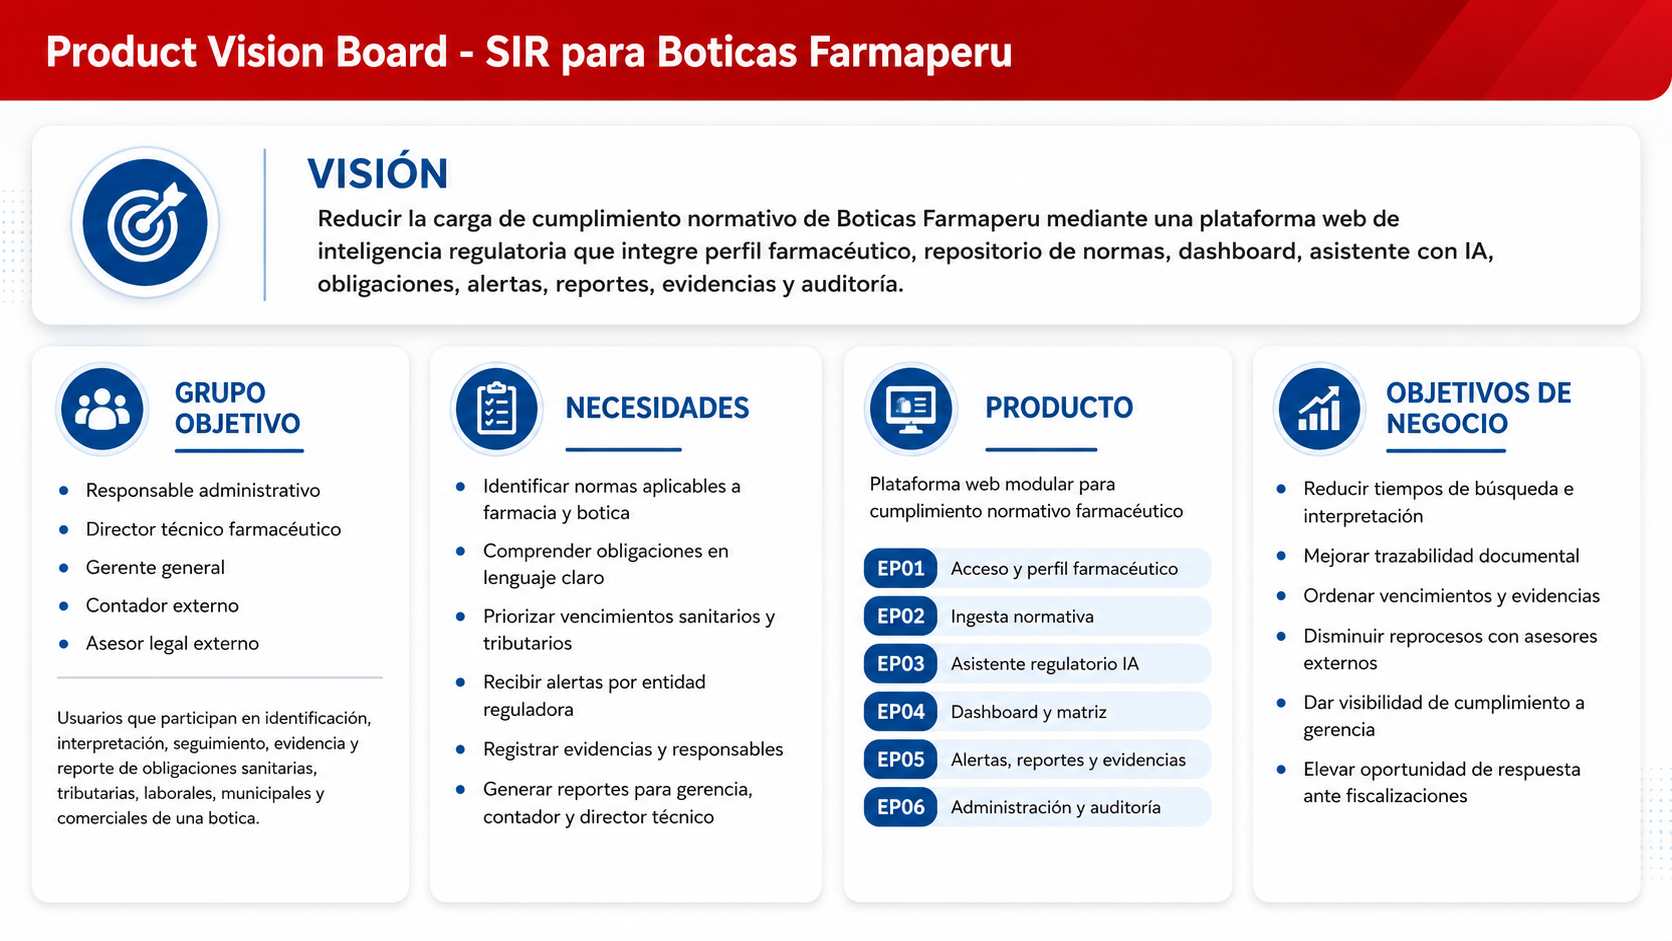
\includegraphics[width=6.5in,height=3.65625in]{figuras/docx_image7.png}

La visión del producto se resume en la siguiente declaración:
implementar una plataforma de inteligencia regulatoria que permita a
Inversiones y Representaciones Peruanas LK S.R.L. (Boticas Farmaperu)
identificar obligaciones aplicables, interpretar cambios normativos en
lenguaje claro, monitorear el estado de cumplimiento, recibir alertas
oportunas y generar reportes con evidencia trazable de las fuentes
oficiales consultadas. Esta visión responde a la necesidad de reducir
tiempos de búsqueda, disminuir dependencia de interpretaciones no
documentadas, ordenar el seguimiento de obligaciones y mejorar la
oportunidad en la toma de decisiones de cumplimiento.

\subsubsection{3.1.2 Perfil del Usuario}\label{perfil-del-usuario}

El usuario principal del sistema es el responsable administrativo de la
PYME, debido a que concentra la coordinación de declaraciones,
licencias, comunicaciones con asesores externos y seguimiento de
obligaciones ante entidades fiscalizadoras. La Figura 6 presenta el
perfil de usuario priorizado, considerando biografía, frase
representativa, personalidad, preocupaciones, frustraciones y
necesidades.

\phantomsection\label{_Toc231672406}{}Figura 6\\
\emph{Perfil del usuario principal}

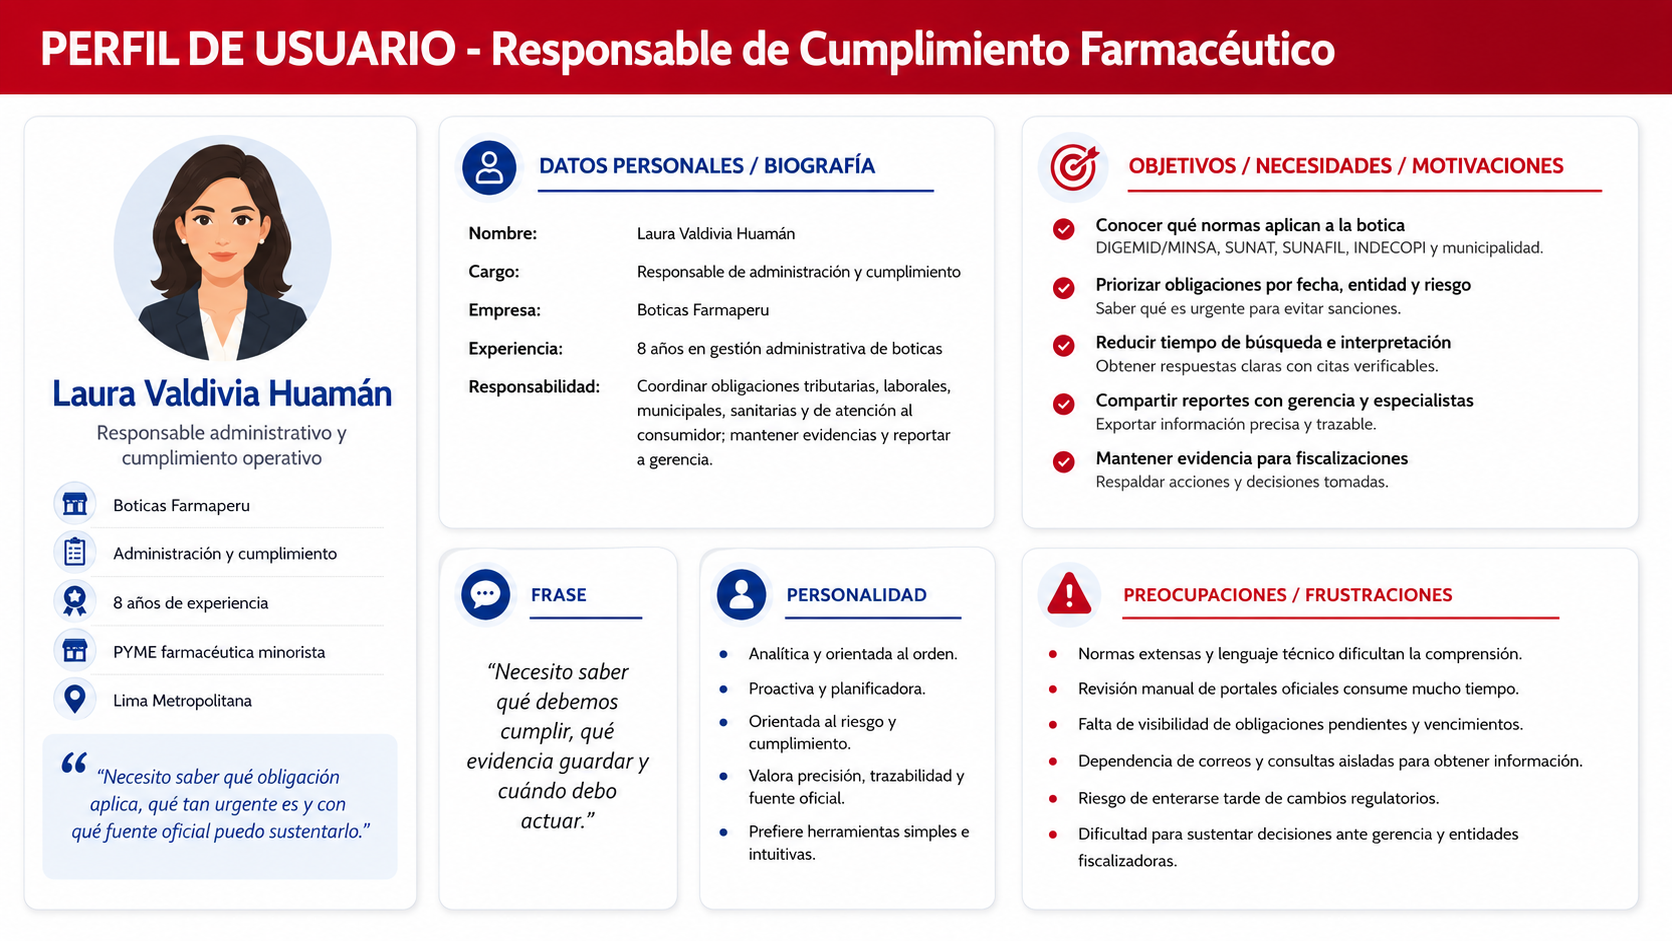
\includegraphics[width=6.5in,height=3.65625in]{figuras/docx_image8.png}

Además del usuario principal, el producto considera usuarios secundarios
que participan en el flujo de cumplimiento normativo. Estos usuarios no
reemplazan el rol del responsable administrativo, pero intervienen en la
revisión, validación o ejecución de acciones derivadas de las respuestas
del SIR.

\phantomsection\label{_Toc231672271}{}Tabla 16\\
\emph{Perfiles de usuario del SIR}

\begin{longtable}[]{@{}
  >{\raggedright\arraybackslash}p{(\columnwidth - 6\tabcolsep) * \real{0.1845}}
  >{\raggedright\arraybackslash}p{(\columnwidth - 6\tabcolsep) * \real{0.1973}}
  >{\raggedright\arraybackslash}p{(\columnwidth - 6\tabcolsep) * \real{0.3321}}
  >{\raggedright\arraybackslash}p{(\columnwidth - 6\tabcolsep) * \real{0.2861}}@{}}
\toprule\noalign{}
\begin{minipage}[b]{\linewidth}\raggedright
\textbf{Perfil}
\end{minipage} & \begin{minipage}[b]{\linewidth}\raggedright
\textbf{Rol en el proceso}
\end{minipage} & \begin{minipage}[b]{\linewidth}\raggedright
\textbf{Necesidad principal}
\end{minipage} & \begin{minipage}[b]{\linewidth}\raggedright
\textbf{Dolor actual}
\end{minipage} \\
\midrule\noalign{}
\endhead
\bottomrule\noalign{}
\endlastfoot
Responsable administrativo & Usuario líder y responsable operativo &
Identificar obligaciones aplicables, fechas relevantes y acciones
concretas de cumplimiento. & Búsqueda manual en múltiples fuentes y
dificultad para interpretar lenguaje legal. \\
Contador externo & Validador tributario y asesor recurrente & Revisar
respuestas, validar obligaciones tributarias y preparar declaraciones. &
Recibe consultas repetitivas y con poca evidencia documental. \\
Gerente general & Decisor y responsable de priorización & Conocer
riesgos de incumplimiento y estado general de obligaciones. & Falta de
visibilidad ejecutiva sobre obligaciones pendientes. \\
Asesor legal externo & Especialista consultado en casos complejos &
Revisar normas de mayor impacto o incertidumbre. & Debe reconstruir
contexto y fuentes antes de emitir opinión. \\
\end{longtable}

\subsubsection{3.1.3 Definición de Roles}\label{definiciuxf3n-de-roles}

El proyecto se organiza bajo un esquema Scrum adaptado al tamaño del
equipo de desarrollo y al alcance funcional de la solución. Los roles
definidos aseguran la separación entre priorización funcional,
coordinación del proceso ágil, desarrollo técnico, validación de calidad
y retroalimentación del usuario líder.

\phantomsection\label{_Toc231672272}{}Tabla 17\\
\emph{Definición de roles del proyecto}

\begin{longtable}[]{@{}
  >{\raggedright\arraybackslash}p{(\columnwidth - 6\tabcolsep) * \real{0.1413}}
  >{\raggedright\arraybackslash}p{(\columnwidth - 6\tabcolsep) * \real{0.2674}}
  >{\raggedright\arraybackslash}p{(\columnwidth - 6\tabcolsep) * \real{0.0996}}
  >{\raggedright\arraybackslash}p{(\columnwidth - 6\tabcolsep) * \real{0.4917}}@{}}
\toprule\noalign{}
\begin{minipage}[b]{\linewidth}\raggedright
\textbf{Rol}
\end{minipage} & \begin{minipage}[b]{\linewidth}\raggedright
\textbf{Responsable}
\end{minipage} & \begin{minipage}[b]{\linewidth}\raggedright
\textbf{Tiempo estimado}
\end{minipage} & \begin{minipage}[b]{\linewidth}\raggedright
\textbf{Responsabilidades}
\end{minipage} \\
\midrule\noalign{}
\endhead
\bottomrule\noalign{}
\endlastfoot
Jefe de Proyecto & Khail Mogollón & 240 horas & Planificar, ejecutar y
controlar el proyecto. Gestionar alcance, cronograma, costos, calidad,
riesgos y comunicaciones. Coordinar con el asesor de tesis, el sponsor
de Boticas Farmaperu y el equipo. Aprobar entregables y reportar avances
quincenales. \\
Product Owner & Ana María Quispe Rojas & 180 horas & Priorizar el
Product Backlog desde la perspectiva del negocio farmacéutico, validar
el valor de cada incremento, aprobar criterios funcionales y mantener
alineada la solución con las necesidades de cumplimiento sanitario,
tributario y operativo de Boticas Farmaperu. \\
Scrum Master & Jadir Hervias & 160 horas & Facilitar ceremonias Scrum,
gestionar impedimentos, promover el cumplimiento del marco ágil y
mantener la visibilidad del avance. \\
Líder técnico & Jadir Hervias & 220 horas & Definir lineamientos de
arquitectura, seleccionar tecnologías y revisar la integración entre
frontend, backend, motor RAG y bases de datos. \\
Analista funcional & Khail Mogollón & 180 horas & Levantar
requerimientos, modelar historias de usuario, criterios de aceptación,
flujos funcionales y reglas de negocio. \\
Desarrollador backend/IA & Jadir Hervias & 300 horas & Implementar API,
ingesta normativa, procesamiento de textos, embeddings, recuperación
vectorial y generación de respuestas. \\
Desarrollador frontend & Khail Mogollón & 260 horas & Implementar
interfaces de perfil empresarial, asistente regulatorio, dashboard,
matriz de obligaciones, alertas, historial y reportes. \\
Analista QA & Equipo de desarrollo & 120 horas & Diseñar y ejecutar
pruebas funcionales, pruebas de precisión, validación de citaciones,
usabilidad y rendimiento. \\
Usuario líder & Responsable administrativo de Inversiones y
Representaciones Peruanas LK S.R.L. (Boticas Farmaperu) & 60 horas &
Validar prototipos, probar flujos del sistema, revisar dashboard,
alertas, reportes, claridad de respuestas y aportar retroalimentación
operativa. \\
Sponsor del proyecto & Gerencia general de Inversiones y
Representaciones Peruanas LK S.R.L. (Boticas Farmaperu) & 40 horas &
Aprobar alcance funcional, facilitar acceso a información operativa y
validar la utilidad del sistema para el seguimiento del cumplimiento y
la toma de decisiones. \\
\end{longtable}

La designación del Product Owner recae en un representante funcional de
la empresa y no en los integrantes del equipo de desarrollo. Esta
separación permite que la priorización del producto responda a
necesidades reales de negocio, mientras que Jadir Hervias y Khail
Mogollón mantienen responsabilidades técnicas y funcionales de
construcción, análisis y validación del sistema.

\subsubsection{3.1.4 Diseño Preliminar de la
Solución}\label{diseuxf1o-preliminar-de-la-soluciuxf3n}

El Product Canvas permite representar de manera integrada el objetivo
del producto, las métricas de éxito, el grupo objetivo, el panorama
general de la solución y los detalles funcionales de alto nivel. La
Figura 7 consolida el diseño preliminar del SIR y establece el puente
entre las necesidades del usuario y las funcionalidades priorizadas en
el Product Backlog.

\phantomsection\label{_Toc231672407}{}Figura 7\\
\emph{Product Canvas}

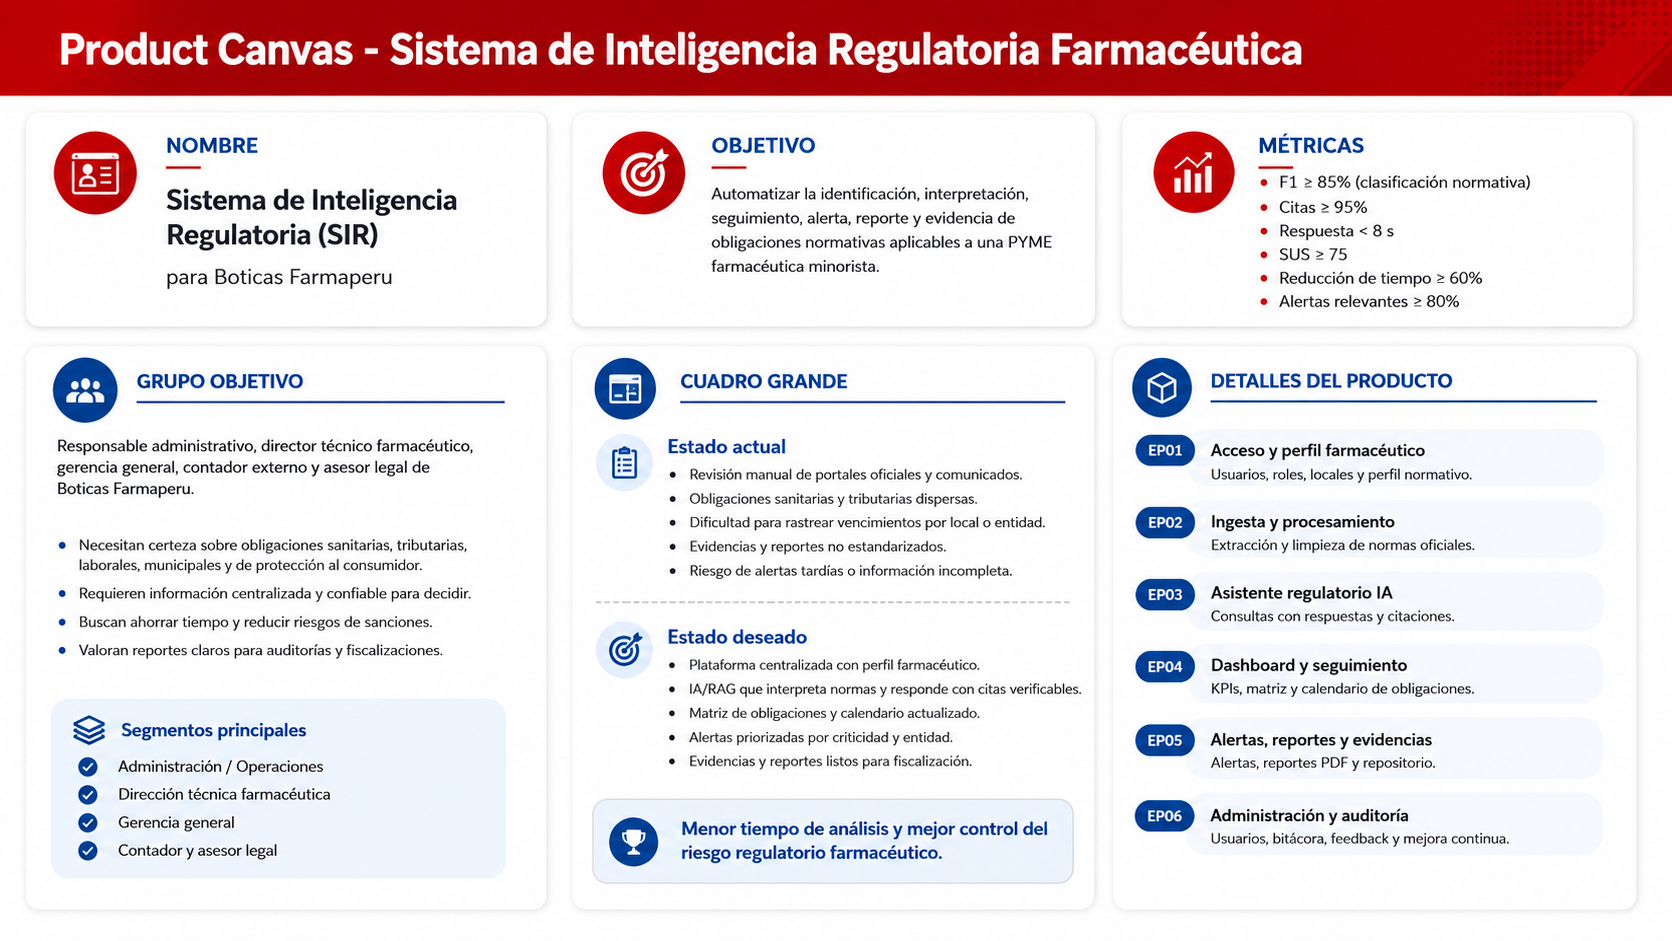
\includegraphics[width=6.5in,height=3.65625in]{figuras/docx_image9.png}

A nivel conceptual, el SIR transforma el proceso de cumplimiento
normativo de la PYME en siete capacidades principales. Primero, permite
configurar un perfil empresarial con rubro, tamaño, ubicación y
entidades reguladoras relevantes. Segundo, automatiza la ingesta y
preparación del corpus normativo. Tercero, habilita consultas en
lenguaje natural con respuestas trazables a fuentes oficiales. Cuarto,
consolida obligaciones en una matriz de seguimiento con responsable,
fecha, estado y evidencia. Quinto, presenta un dashboard ejecutivo con
semáforos, indicadores y alertas por vencer. Sexto, genera reportes
exportables para gerencia, contador externo o asesor legal. Séptimo,
organiza evidencias, historial, auditoría y retroalimentación para
sostener la mejora continua del proceso de cumplimiento.

\phantomsection\label{_Toc231672273}{}Tabla 18\\
\emph{Módulos funcionales de la solución SIR}

\begin{longtable}[]{@{}
  >{\raggedright\arraybackslash}p{(\columnwidth - 4\tabcolsep) * \real{0.2020}}
  >{\raggedright\arraybackslash}p{(\columnwidth - 4\tabcolsep) * \real{0.4218}}
  >{\raggedright\arraybackslash}p{(\columnwidth - 4\tabcolsep) * \real{0.3762}}@{}}
\toprule\noalign{}
\begin{minipage}[b]{\linewidth}\raggedright
\textbf{Módulo}
\end{minipage} & \begin{minipage}[b]{\linewidth}\raggedright
\textbf{Propósito}
\end{minipage} & \begin{minipage}[b]{\linewidth}\raggedright
\textbf{Valor para la PYME}
\end{minipage} \\
\midrule\noalign{}
\endhead
\bottomrule\noalign{}
\endlastfoot
Perfil empresarial y normativo & Registrar rubro, tamaño, ubicación,
entidades reguladoras y preferencias. & Permite contextualizar
consultas, alertas y obligaciones según la realidad de la empresa. \\
Repositorio normativo & Ingerir, limpiar, clasificar y almacenar normas
oficiales y fragmentos relevantes. & Reduce búsqueda manual y centraliza
fuentes consultables. \\
Asistente regulatorio con IA & Responder consultas en lenguaje natural
mediante RAG y citas verificables. & Facilita interpretación operativa
sin perder trazabilidad de fuentes. \\
Dashboard de cumplimiento & Mostrar indicadores, obligaciones
pendientes, alertas y semáforos por entidad. & Brinda visibilidad
ejecutiva para priorizar acciones de cumplimiento. \\
Matriz de obligaciones & Registrar obligación, responsable, vencimiento,
estado, evidencia y comentarios. & Convierte una respuesta normativa en
una acción gestionable. \\
Sistema básico de alertas & Notificar cambios normativos, obligaciones
por vencer y pendientes críticos. & Mejora la oportunidad de respuesta
ante riesgos de incumplimiento. \\
Reportes ejecutivos & Generar reportes PDF con consultas, respuestas,
fuentes, estados y conclusiones operativas. & Facilita la comunicación
con gerencia, contador y asesor legal. \\
Repositorio de evidencias & Centralizar archivos, enlaces, constancias,
capturas, respuestas y documentos asociados a cada obligación. & Permite
sustentar acciones de cumplimiento y reducir pérdida de información. \\
Historial, auditoría y mejora continua & Registrar consultas,
citaciones, reportes, calificaciones, cambios y acciones de usuarios. &
Permite aprendizaje continuo, control interno y revisión posterior. \\
\end{longtable}

\subsubsection{3.1.5 Prototipos Alto Nivel}\label{prototipos-alto-nivel}

Los prototipos de alto nivel representan las pantallas principales de la
solución. No constituyen diseños finales de interfaz, sino artefactos
funcionales que permiten validar navegación, estructura de información y
acciones clave del usuario. La Figura 8 muestra los prototipos
correspondientes al dashboard de cumplimiento, asistente regulatorio con
IA, matriz de obligaciones, centro de alertas, reportes, repositorio de
evidencias y perfil normativo de la empresa.

\phantomsection\label{_Toc231672408}{}Figura 8\\
\emph{Prototipos de alto nivel}

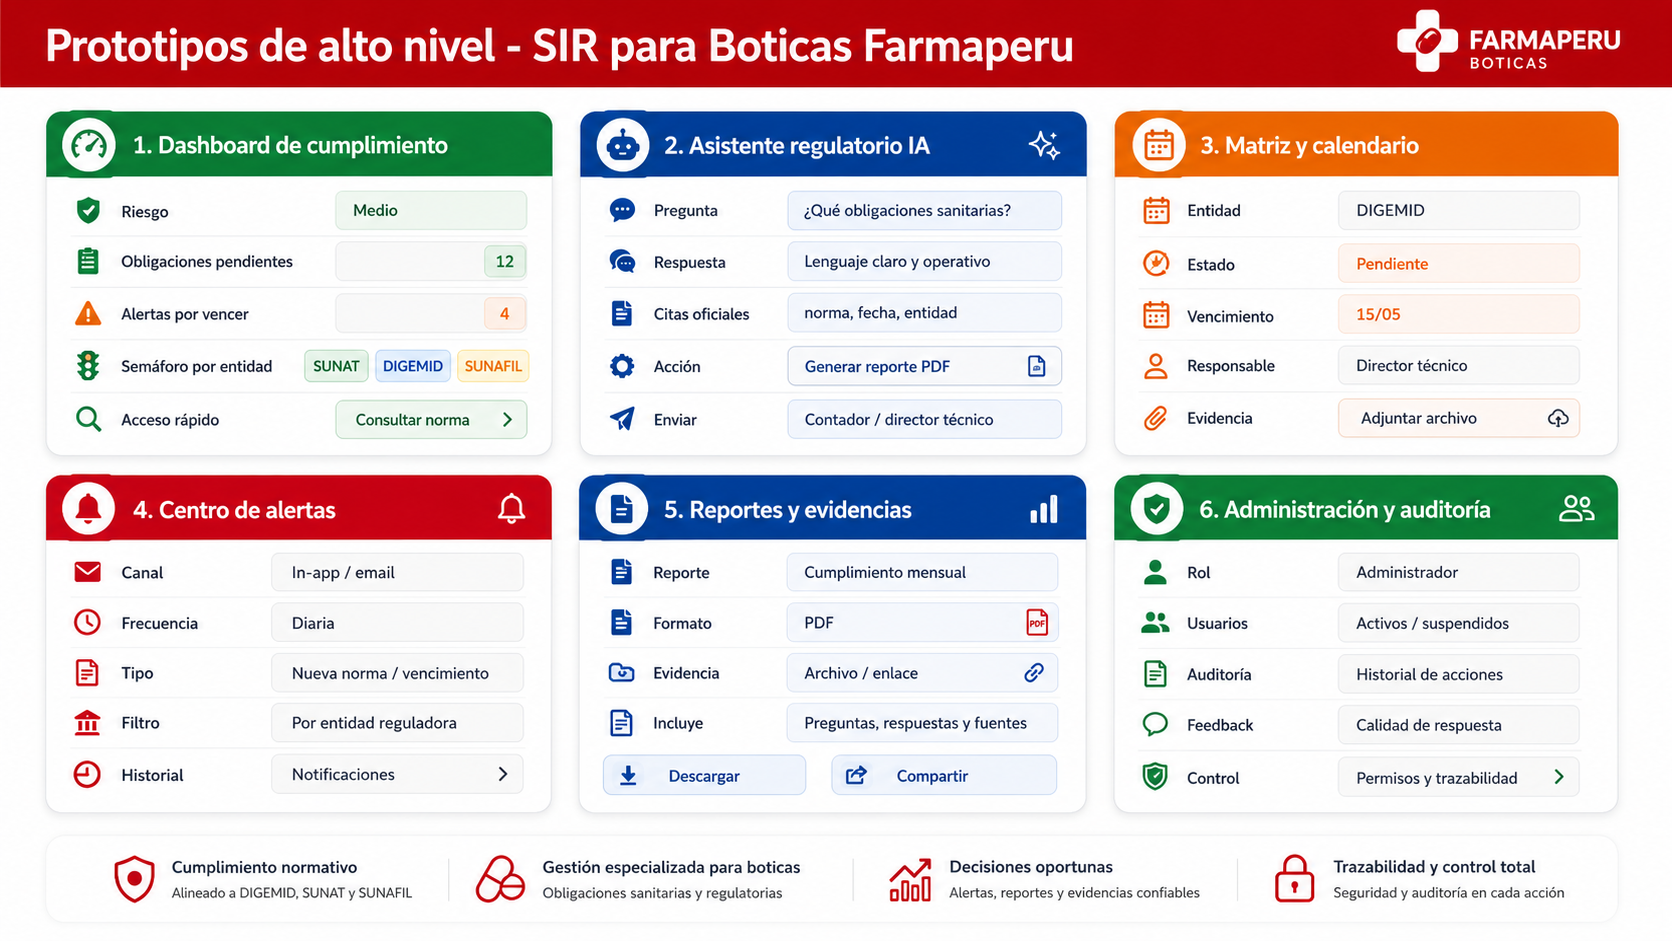
\includegraphics[width=6.28403in,height=3.53476in]{figuras/docx_image10.png}

Las épicas funcionales asociadas a los prototipos son las siguientes:

\begin{itemize}
\item
  \textbf{Épica 1: Gestión de acceso y perfil empresarial.} Permite
  registrar usuarios, autenticar accesos, administrar roles iniciales y
  configurar los datos base de la empresa.
\item
  \textbf{Épica 2: Ingesta y procesamiento normativo.} Permite
  recolectar, limpiar, segmentar, clasificar y vectorizar normas
  oficiales para alimentar el repositorio normativo.
\item
  \textbf{Épica 3: Asistente regulatorio con IA.} Permite realizar
  preguntas en lenguaje natural, recibir respuestas con citas
  verificables y contextualizar la interpretación según el perfil de la
  PYME.
\item
  \textbf{Épica 4: Dashboard y seguimiento de obligaciones.} Permite
  visualizar indicadores de cumplimiento, semáforos por entidad,
  obligaciones pendientes y calendario de vencimientos.
\item
  \textbf{Épica 5: Alertas, reportes y evidencias de cumplimiento.}
  Permite configurar alertas básicas, generar reportes PDF, adjuntar
  evidencias y organizar documentos de sustento por obligación.
\item
  \textbf{Épica 6: Administración, auditoría y mejora continua.} Permite
  gestionar usuarios, permisos, historial de consultas, trazabilidad de
  acciones y retroalimentación para mejorar la calidad del sistema.
\end{itemize}

\subsubsection{}\label{section}

\subsubsection{3.1.6 Historias de Usuario}\label{historias-de-usuario}

Las historias de usuario se formulan con la estructura: Como rol,
necesito funcionalidad, para obtener valor de negocio. Esta estructura
permite conectar las necesidades del usuario con entregables
verificables y criterios de aceptación medibles.

\phantomsection\label{_Toc231672274}{}Tabla 19\\
\emph{Descripción de historias de usuario}

\begin{longtable}[]{@{}
  >{\raggedright\arraybackslash}p{(\columnwidth - 12\tabcolsep) * \real{0.0291}}
  >{\raggedright\arraybackslash}p{(\columnwidth - 12\tabcolsep) * \real{0.1211}}
  >{\raggedright\arraybackslash}p{(\columnwidth - 12\tabcolsep) * \real{0.1056}}
  >{\raggedright\arraybackslash}p{(\columnwidth - 12\tabcolsep) * \real{0.1283}}
  >{\raggedright\arraybackslash}p{(\columnwidth - 12\tabcolsep) * \real{0.1846}}
  >{\raggedright\arraybackslash}p{(\columnwidth - 12\tabcolsep) * \real{0.1938}}
  >{\raggedright\arraybackslash}p{(\columnwidth - 12\tabcolsep) * \real{0.2374}}@{}}
\toprule\noalign{}
\multirow{2}{=}{\begin{minipage}[b]{\linewidth}\raggedright
\textbf{N.º}
\end{minipage}} &
\multirow{2}{=}{\begin{minipage}[b]{\linewidth}\raggedright
\textbf{Épica}
\end{minipage}} &
\multirow{2}{=}{\begin{minipage}[b]{\linewidth}\raggedright
\textbf{Identificador Historia}
\end{minipage}} &
\multirow{2}{=}{\begin{minipage}[b]{\linewidth}\raggedright
\textbf{Nombre de la historia}
\end{minipage}} &
\multicolumn{3}{>{\raggedright\arraybackslash}p{(\columnwidth - 12\tabcolsep) * \real{0.6158} + 4\tabcolsep}@{}}{%
\begin{minipage}[b]{\linewidth}\raggedright
\textbf{Descripción de la historia de usuario}
\end{minipage}} \\
& & & & \begin{minipage}[b]{\linewidth}\raggedright
\textbf{Como (rol)}
\end{minipage} & \begin{minipage}[b]{\linewidth}\raggedright
\textbf{Necesito (característica)}
\end{minipage} & \begin{minipage}[b]{\linewidth}\raggedright
\textbf{Para (valor de negocio)}
\end{minipage} \\
\midrule\noalign{}
\endhead
\bottomrule\noalign{}
\endlastfoot
1 & \multirow{3}{=}{EP01 - Gestión de acceso y perfil empresarial} &
HU01 & Registro de usuario y empresa & Responsable administrativo &
registrar mi usuario y los datos básicos de la empresa & acceder al SIR
con una cuenta segura y vinculada a Boticas Farmaperu. \\
2 & & HU02 & Autenticación y roles & Usuario registrado & iniciar y
cerrar sesión de forma segura & usar únicamente las funciones
autorizadas según mi rol. \\
3 & & HU03 & Configuración de perfil normativo & Responsable
administrativo & configurar rubro, tamaño, ubicación y entidades
reguladoras & recibir información normativa aplicable a la realidad de
la PYME. \\
4 & \multirow{4}{=}{EP02 - Ingesta y procesamiento normativo} & HU04 &
Ingesta automática de normas & Sistema & extraer normas oficiales desde
El Peruano, fuentes locales y URL oficiales & mantener actualizado el
corpus normativo con trazabilidad de origen. \\
5 & & HU05 & Limpieza y normalización textual & Sistema & convertir PDF,
HTML o TXT a texto legal limpio y segmentado & preparar documentos
confiables para recuperación semántica. \\
6 & & HU06 & Vectorización de documentos & Sistema & generar embeddings
de fragmentos normativos con API de embeddings y almacenarlos en
pgvector & habilitar búsqueda semántica trazable dentro del SIR. \\
7 & & HU07 & Clasificación normativa & Sistema & clasificar normas por
entidad, rubro, tipo de norma y obligación & mejorar la relevancia de
recuperación y priorización regulatoria. \\
8 & \multirow{3}{=}{EP03 - Asistente regulatorio con IA} & HU08 &
Consulta en lenguaje natural & Responsable administrativo & formular
preguntas en lenguaje natural sobre obligaciones normativas & comprender
acciones de cumplimiento sin leer documentos extensos. \\
9 & & HU09 & Respuestas con citas verificables & Usuario del SIR &
recibir respuestas con fuente oficial, fragmento y metadatos
verificables & validar la información usada antes de tomar una
decisión. \\
10 & & HU10 & Consulta contextualizada & Usuario PYME & obtener
respuestas que consideren el perfil normativo de la empresa & saber si
una norma aplica, no aplica o requiere revisión especializada. \\
11 & \multirow{3}{=}{EP04 - Dashboard y seguimiento de obligaciones} &
HU11 & Dashboard de cumplimiento & Gerente general & visualizar
indicadores, riesgos, alertas y obligaciones recientes & conocer el
estado de cumplimiento y priorizar decisiones. \\
12 & & HU14 & Seguimiento de obligaciones & Responsable administrativo &
registrar estado, responsable, fecha y evidencia de cada obligación &
controlar el cumplimiento y reducir omisiones operativas. \\
13 & & HU19 & Calendario de vencimientos & Responsable administrativo &
visualizar obligaciones por fecha de vencimiento & priorizar acciones y
evitar incumplimientos por demora. \\
14 & \multirow{4}{=}{EP05 - Alertas, reportes y evidencias de
cumplimiento} & HU12 & Alertas regulatorias & Responsable administrativo
& recibir alertas sobre cambios normativos y obligaciones próximas &
actuar oportunamente ante riesgos de incumplimiento. \\
15 & & HU13 & Preferencias de notificación & Usuario del SIR &
configurar frecuencia, entidades, prioridad y canal de alertas & recibir
información útil sin saturación de notificaciones. \\
16 & & HU15 & Exportación de reportes & Contador externo & exportar
respuestas, fuentes, obligaciones y evidencias a PDF & sustentar
revisiones, declaraciones y decisiones de cumplimiento. \\
17 & & HU20 & Repositorio de evidencias & Responsable administrativo &
adjuntar y consultar documentos de sustento asociados a obligaciones &
mantener evidencia ordenada y recuperable ante revisiones. \\
18 & \multirow{3}{=}{EP06 - Administración, auditoría y mejora continua}
& HU16 & Historial y auditoría & Usuario del SIR & consultar historial
de preguntas, respuestas, fuentes y acciones & reutilizar evidencia y
revisar decisiones tomadas. \\
19 & & HU17 & Feedback de respuestas & Usuario líder & calificar
utilidad, reportar errores y comentar respuestas & mejorar la calidad
del sistema y del dataset de validación. \\
20 & & HU18 & Administración de usuarios & Administrador & crear,
editar, suspender usuarios y asignar roles & mantener control de accesos
y segregación de funciones. \\
\end{longtable}

\paragraph{3.1.6.1 Criterios de
aceptación}\label{criterios-de-aceptaciuxf3n}

Los criterios de aceptación establecen las condiciones mínimas que debe
cumplir cada historia para ser considerada terminada. Se priorizan
criterios verificables en pruebas funcionales, pruebas de integración,
revisión de trazabilidad y validación con el usuario líder.

\phantomsection\label{_Toc231672275}{}Tabla 20\\
\emph{Criterios de aceptación principales}

\begin{longtable}[]{@{}
  >{\raggedright\arraybackslash}p{(\columnwidth - 4\tabcolsep) * \real{0.0896}}
  >{\raggedright\arraybackslash}p{(\columnwidth - 4\tabcolsep) * \real{0.1845}}
  >{\raggedright\arraybackslash}p{(\columnwidth - 4\tabcolsep) * \real{0.7259}}@{}}
\toprule\noalign{}
\begin{minipage}[b]{\linewidth}\raggedright
\textbf{ID}
\end{minipage} & \begin{minipage}[b]{\linewidth}\raggedright
\textbf{Historia}
\end{minipage} & \begin{minipage}[b]{\linewidth}\raggedright
\textbf{Criterios de aceptación}
\end{minipage} \\
\midrule\noalign{}
\endhead
\bottomrule\noalign{}
\endlastfoot
HU01 & Registro de usuario y empresa &
\begin{minipage}[t]{\linewidth}\raggedright
\begin{itemize}
\item
  El formulario debe solicitar correo, contraseña, razón social y RUC;
  debe validar correo válido, razón social de 2 a 255 caracteres, RUC de
  exactamente 11 dígitos y contraseña de 12 a 128 caracteres con
  mayúscula, minúscula, número y carácter especial.
\item
  Al registrar correctamente, el sistema debe crear la empresa, crear el
  usuario con rol RESPONSABLE\_ADMINISTRATIVO, guardar la contraseña con
  hash Argon2 y registrar fecha de creación.
\item
  Si el correo o el RUC ya existen, debe responder con error 409 y no
  debe crear registros parciales.
\item
  Al finalizar el registro, debe iniciar sesión mediante cookie JWT
  HttpOnly y mostrar mensaje de creación exitosa en un tiempo operativo
  menor a 2 segundos en ambiente de validación.
\end{itemize}
\end{minipage} \\
HU02 & Autenticación y roles &
\begin{minipage}[t]{\linewidth}\raggedright
\begin{itemize}
\item
  La pantalla de login debe exigir correo y contraseña; credenciales
  inválidas, usuario inactivo o token expirado deben devolver error 401
  sin exponer cuál dato falló.
\item
  La sesión debe emitirse mediante JWT en cookie HttpOnly con expiración
  configurada y debe cerrarse eliminando la cookie con respuesta 204.
\item
  El sistema debe exponer permisos por rol y bloquear rutas protegidas
  con error 401 cuando no exista sesión y 403 cuando el rol no tenga
  autorización.
\item
  La recuperación de contraseña debe generar un token de uso único, con
  vigencia de 30 minutos; token inválido, usado o vencido debe ser
  rechazado y la nueva contraseña debe cumplir la política de seguridad.
\end{itemize}
\end{minipage} \\
HU03 & Configuración de perfil normativo &
\begin{minipage}[t]{\linewidth}\raggedright
\begin{itemize}
\item
  El perfil debe registrar rubro/CIIU, tamaño empresarial, régimen
  tributario, ubicación, número de trabajadores, canales de venta y
  entidades reguladoras de interés.
\item
  Debe impedir guardar el perfil cuando falten campos obligatorios o
  cuando los valores no pertenezcan a catálogos válidos.
\item
  Cada cambio debe conservar usuario, fecha, campos modificados y valor
  anterior/nuevo para auditoría.
\item
  Si el perfil está incompleto, el sistema debe advertirlo y evitar que
  las respuestas se presenten como plenamente contextualizadas.
\end{itemize}
\end{minipage} \\
HU04 & Ingesta automática de normas &
\begin{minipage}[t]{\linewidth}\raggedright
\begin{itemize}
\item
  El sistema debe permitir crear, pausar, reactivar y ejecutar fuentes
  de ingesta con nombre, URL, periodicidad y estado; una URL duplicada
  debe devolver error 409.
\item
  Para El Peruano, la fuente diaria debe resolver la fecha de Lima,
  reiniciar start=0, conservar entidad Salud y tipoPublicacion=NL,
  paginar resultados y crear trabajos hijos deduplicados por norma
  encontrada.
\item
  La ejecución manual por rango debe validar que la fecha final sea
  igual o posterior a la inicial; si la fuente no corresponde a búsqueda
  de El Peruano debe devolver error 422 y no alterar la programación
  automática.
\item
  La ingesta debe descargar PDF o HTML, aplicar fallback cuando el PDF
  no esté disponible, calcular SHA-256, almacenar metadatos de fuente y
  registrar logs de inicio, descarga, deduplicación, éxito o error.
\item
  La carga manual solo debe aceptar PDF, HTML, HTM o TXT y rechazar
  archivos no permitidos con 400 o archivos mayores al límite
  configurado con 413.
\end{itemize}
\end{minipage} \\
HU05 & Limpieza y normalización textual &
\begin{minipage}[t]{\linewidth}\raggedright
\begin{itemize}
\item
  El sistema debe extraer texto desde PDF, HTML o TXT y normalizar
  Unicode NFKC, saltos de línea y espacios para generar texto legal
  limpio.
\item
  Debe eliminar ruido como encabezados repetitivos, scripts, estilos,
  navegación, líneas vacías excesivas y texto duplicado corto, sin
  eliminar artículos, disposiciones, títulos, capítulos o anexos.
\item
  Debe segmentar el texto en fragmentos con índice, encabezado y tipo de
  sección; los fragmentos grandes deben dividirse respetando párrafos u
  oraciones y solapamiento controlado.
\item
  Si no se extrae texto útil o no se generan fragmentos, el trabajo debe
  quedar en estado FAILED con mensaje de error y log técnico trazable.
\end{itemize}
\end{minipage} \\
HU06 & Vectorización de documentos &
\begin{minipage}[t]{\linewidth}\raggedright
\begin{itemize}
\item
  El TO-BE final debe generar embeddings mediante API de embeddings/LLM;
  en Sprint 1 se usa OpenAI text-embedding-3-large con 1536 dimensiones,
  y el fallback local queda limitado a pruebas o desarrollo cuando no
  exista clave.
\item
  Cada embedding debe asociarse a un fragmento normativo y guardarse en
  norm\_chunks.embedding de PostgreSQL con pgvector, manteniendo
  metadata de documento, fuente, norma, entidad, fecha, proveedor y
  modelo.
\item
  La base debe crear extensión pgvector e índice HNSW de distancia
  coseno cuando la dimensión lo permite, para recuperar Top-K de forma
  eficiente.
\item
  La búsqueda semántica debe rechazar consultas vacías con 400, limitar
  resultados entre 1 y 20, y devolver fragmento, metadatos y score de
  similitud.
\item
  Si el proveedor de embeddings falla, el trabajo debe registrar el
  error, quedar en FAILED y no marcar el documento como procesado.
\end{itemize}
\end{minipage} \\
HU07 & Clasificación normativa &
\begin{minipage}[t]{\linewidth}\raggedright
\begin{itemize}
\item
  El clasificador debe asignar entidad emisora, tipo de norma, rubro
  afectado, tipo de obligación y nivel de impacto a cada documento o
  fragmento.
\item
  La clasificación debe usar metadatos extraídos y contenido textual;
  cuando la confianza sea menor al umbral definido debe marcar el
  registro como ``requiere revisión''.
\item
  El usuario autorizado debe poder corregir manualmente una
  clasificación y el sistema debe guardar el cambio con usuario y fecha.
\item
  Las clasificaciones deben quedar disponibles para filtros del corpus,
  dashboard, alertas y consultas RAG.
\end{itemize}
\end{minipage} \\
HU08 & Consulta en lenguaje natural &
\begin{minipage}[t]{\linewidth}\raggedright
\begin{itemize}
\item
  El asistente debe aceptar preguntas en español, validar que la
  consulta no esté vacía y procesar preguntas relacionadas con
  obligaciones tributarias, laborales, sanitarias, municipales o de
  consumidor.
\item
  Debe recuperar fragmentos relevantes del corpus y generar una
  respuesta operativa en menos de 8 segundos bajo carga normal de
  validación.
\item
  Si no existe evidencia suficiente, debe responder que no cuenta con
  información suficiente y sugerir revisar con contador, asesor o fuente
  oficial.
\item
  Debe registrar la consulta, usuario, fecha, fragmentos recuperados y
  resultado para auditoría y mejora continua.
\end{itemize}
\end{minipage} \\
HU09 & Respuestas con citas verificables &
\begin{minipage}[t]{\linewidth}\raggedright
\begin{itemize}
\item
  Toda respuesta que use contenido normativo debe incluir fuente
  oficial, entidad, fecha, número o título de norma, fragmento citado y
  URL o documento de origen cuando esté disponible.
\item
  Durante validación, al menos 95 \% de las respuestas aceptadas deben
  tener citación verificable.
\item
  Si una fuente no posee URL oficial o metadatos completos, el sistema
  debe mostrar la limitación y no ocultar la incertidumbre.
\item
  La respuesta debe incluir aviso de apoyo interpretativo no vinculante
  y no debe presentarse como asesoría legal definitiva.
\end{itemize}
\end{minipage} \\
HU10 & Consulta contextualizada &
\begin{minipage}[t]{\linewidth}\raggedright
\begin{itemize}
\item
  La respuesta debe considerar rubro, tamaño, ubicación, régimen
  tributario, número de trabajadores y entidades asociadas al perfil
  empresarial.
\item
  Debe clasificar la aplicabilidad como ``aplica'', ``no aplica'' o
  ``requiere revisión'', explicando la condición usada para decidir.
\item
  Si el perfil está incompleto o desactualizado, debe solicitar
  completar datos antes de emitir una conclusión contextual.
\item
  La contextualización debe quedar registrada para permitir auditoría de
  la decisión y comparación con validación humana.
\end{itemize}
\end{minipage} \\
HU11 & Dashboard de cumplimiento &
\begin{minipage}[t]{\linewidth}\raggedright
\begin{itemize}
\item
  El dashboard debe mostrar documentos procesados, fragmentos, trabajos
  pendientes, en ejecución y fallidos, disponibilidad del repositorio
  vectorial y proveedor de embeddings.
\item
  Debe listar obligaciones, alertas y riesgos por entidad o estado
  cuando existan datos en el sistema.
\item
  Cuando no existan datos, debe mostrar estado vacío comprensible y
  accesos para iniciar ingesta o configuración.
\item
  Los indicadores deben actualizarse al cargar la pantalla y reflejar la
  información persistida en la base de datos.
\end{itemize}
\end{minipage} \\
HU14 & Seguimiento de obligaciones &
\begin{minipage}[t]{\linewidth}\raggedright
\begin{itemize}
\item
  Cada obligación debe permitir registrar responsable, prioridad,
  estado, fecha de vencimiento, fecha de atención, comentarios y
  evidencia asociada.
\item
  Los estados mínimos deben incluir pendiente, en proceso, atendida,
  vencida y descartada con justificación.
\item
  No debe permitirse marcar una obligación como atendida sin fecha de
  atención ni evidencia o comentario de sustento.
\item
  Todo cambio de estado debe registrar usuario, fecha y valor
  anterior/nuevo para auditoría.
\end{itemize}
\end{minipage} \\
HU19 & Calendario de vencimientos &
\begin{minipage}[t]{\linewidth}\raggedright
\begin{itemize}
\item
  El calendario debe mostrar obligaciones en vista mensual y semanal,
  con filtros por entidad, responsable, prioridad y estado.
\item
  Los vencimientos próximos y vencidos deben resaltarse con semáforo o
  indicador visual.
\item
  Las obligaciones sin fecha de vencimiento deben aparecer en una
  bandeja de revisión para que el usuario complete la fecha o descarte
  el registro.
\item
  Al seleccionar una obligación, el usuario debe acceder a detalle,
  fuente, responsable y evidencia vinculada.
\end{itemize}
\end{minipage} \\
HU12 & Alertas regulatorias &
\begin{minipage}[t]{\linewidth}\raggedright
\begin{itemize}
\item
  El sistema debe generar alertas ante nuevas normas relevantes, cambios
  de estado y obligaciones próximas a vencer según umbrales
  configurados.
\item
  Debe evitar alertas duplicadas para el mismo evento, fuente y usuario
  dentro del periodo configurado.
\item
  Las alertas deben registrar fecha de creación, prioridad, entidad,
  obligación relacionada y estado de lectura.
\item
  Si el canal de envío falla, debe conservar la alerta en el sistema y
  registrar el error para reintento o revisión.
\end{itemize}
\end{minipage} \\
HU13 & Preferencias de notificación &
\begin{minipage}[t]{\linewidth}\raggedright
\begin{itemize}
\item
  El usuario debe poder activar o desactivar alertas por entidad, tipo
  de obligación, prioridad, frecuencia y canal.
\item
  Los cambios de preferencias deben aplicarse a nuevas alertas sin
  eliminar el historial existente.
\item
  Si el canal configurado no es válido o está incompleto, el sistema
  debe advertirlo y no guardar una configuración inconsistente.
\item
  El usuario debe poder pausar notificaciones automáticas sin impedir
  consultas manuales ni revisión de alertas en pantalla.
\end{itemize}
\end{minipage} \\
HU15 & Exportación de reportes &
\begin{minipage}[t]{\linewidth}\raggedright
\begin{itemize}
\item
  El reporte PDF debe incluir pregunta, respuesta, fuentes, fecha de
  emisión, usuario, perfil empresarial usado, obligaciones relacionadas,
  evidencias y aviso de apoyo no vinculante.
\item
  Debe generarse en menos de 10 segundos para reportes estándar de hasta
  20 consultas u obligaciones.
\item
  Si faltan citaciones o evidencias necesarias, el sistema debe marcar
  la sección como incompleta y no ocultar la ausencia.
\item
  El reporte debe poder descargarse y quedar registrado en historial
  para auditoría posterior.
\end{itemize}
\end{minipage} \\
HU20 & Repositorio de evidencias &
\begin{minipage}[t]{\linewidth}\raggedright
\begin{itemize}
\item
  El repositorio debe permitir adjuntar archivos o enlaces a una
  obligación, consulta o reporte, registrando tipo de evidencia,
  usuario, fecha y descripción.
\item
  Debe validar tipo y tamaño máximo de archivo, y rechazar extensiones
  no permitidas con mensaje claro.
\item
  Cada evidencia debe poder consultarse, descargarse y relacionarse con
  la obligación o respuesta que sustenta.
\item
  La eliminación o reemplazo de evidencias debe quedar auditada y no
  debe borrar el historial de trazabilidad.
\end{itemize}
\end{minipage} \\
HU16 & Historial y auditoría &
\begin{minipage}[t]{\linewidth}\raggedright
\begin{itemize}
\item
  El historial debe listar consultas, respuestas, fuentes usadas,
  acciones de ingesta, reportes y cambios de obligaciones con usuario y
  fecha.
\item
  Debe permitir búsqueda por palabra clave, rango de fechas, entidad y
  usuario, respetando permisos por rol.
\item
  Las acciones críticas deben conservar valor anterior y valor nuevo
  cuando corresponda.
\item
  Los usuarios sin permiso no deben acceder al historial de otros
  usuarios ni a eventos administrativos.
\end{itemize}
\end{minipage} \\
HU17 & Feedback de respuestas &
\begin{minipage}[t]{\linewidth}\raggedright
\begin{itemize}
\item
  El usuario debe poder calificar una respuesta de 1 a 5 y registrar
  comentario, categoría de error o utilidad percibida.
\item
  Debe permitirse un feedback principal por respuesta y actualizarlo sin
  duplicar registros.
\item
  El feedback debe quedar asociado a consulta, fuentes recuperadas,
  usuario y fecha para análisis de calidad.
\item
  Los comentarios vacíos deben aceptarse solo si existe calificación;
  reportes de error deben exigir categoría.
\end{itemize}
\end{minipage} \\
HU18 & Administración de usuarios &
\begin{minipage}[t]{\linewidth}\raggedright
\begin{itemize}
\item
  El administrador debe poder crear, editar, activar, suspender usuarios
  y asignar roles permitidos sin visualizar contraseñas en texto plano.
\item
  Solo usuarios con permiso administrativo deben acceder a la gestión de
  usuarios; otros roles deben recibir 403.
\item
  No debe permitirse suspender al único administrador activo ni dejar la
  empresa sin usuario con capacidad de administración.
\item
  Los cambios de rol o estado deben registrarse en auditoría con usuario
  ejecutor, fecha y valores modificados.
\end{itemize}
\end{minipage} \\
\end{longtable}

\subsubsection{3.1.7 Product Backlog Base}\label{product-backlog-base}

\paragraph{3.1.7.1 Técnica de
priorización}\label{tuxe9cnica-de-priorizaciuxf3n}

Para ordenar el desarrollo de las historias de usuario se utiliza la
técnica MoSCoW. Los requisitos \emph{Must} \emph{Have} son
indispensables para demostrar la solución mínima viable; los
\emph{Should Have} aportan valor relevante, pero pueden implementarse
después del núcleo funcional; los Could Have son mejoras deseables para
ampliar la experiencia de usuario, la trazabilidad o la administración.

\paragraph{3.1.7.2 Técnica de
estimación}\label{tuxe9cnica-de-estimaciuxf3n}

La estimación del esfuerzo se realiza mediante \emph{Planning Poker},
asignando puntos de historia según complejidad funcional, incertidumbre
técnica, dependencias y riesgo de integración. La estimación se expresa
en una escala relativa y permite planificar el alcance de los cuatro
sprints del proyecto.

\phantomsection\label{_Toc231672276}{}Tabla 21\\
\emph{Listado de historias de usuario ordenado por identificador}

\begin{longtable}[]{@{}
  >{\raggedright\arraybackslash}p{(\columnwidth - 4\tabcolsep) * \real{0.1964}}
  >{\raggedright\arraybackslash}p{(\columnwidth - 4\tabcolsep) * \real{0.1813}}
  >{\raggedright\arraybackslash}p{(\columnwidth - 4\tabcolsep) * \real{0.6223}}@{}}
\toprule\noalign{}
\begin{minipage}[b]{\linewidth}\raggedright
ID
\end{minipage} & \begin{minipage}[b]{\linewidth}\raggedright
Épica
\end{minipage} & \begin{minipage}[b]{\linewidth}\raggedright
Nombre de la historia
\end{minipage} \\
\midrule\noalign{}
\endhead
\bottomrule\noalign{}
\endlastfoot
HU01 & EP01 & Registro de usuario y empresa \\
HU02 & EP01 & Autenticación y roles \\
HU03 & EP01 & Configuración de perfil normativo \\
HU04 & EP02 & Ingesta automática de normas \\
HU05 & EP02 & Limpieza y normalización textual \\
HU06 & EP02 & Vectorización de documentos \\
HU07 & EP02 & Clasificación normativa \\
HU08 & EP03 & Consulta en lenguaje natural \\
HU09 & EP03 & Respuestas con citas verificables \\
HU10 & EP03 & Consulta contextualizada \\
HU11 & EP04 & Dashboard de cumplimiento \\
HU12 & EP05 & Alertas regulatorias \\
HU13 & EP05 & Preferencias de notificación \\
HU14 & EP04 & Seguimiento de obligaciones \\
HU15 & EP05 & Exportación de reportes \\
HU16 & EP06 & Historial y auditoría \\
HU17 & EP06 & Feedback de respuestas \\
HU18 & EP06 & Administración de usuarios \\
HU19 & EP04 & Calendario de vencimientos \\
HU20 & EP05 & Repositorio de evidencias \\
\end{longtable}

Posteriormente, se presenta el mismo conjunto de historias ordenado por
valor de negocio y prioridad MoSCoW, lo que define la asignación de cada
historia a su sprint correspondiente.

\phantomsection\label{_Toc231672277}{}Tabla 22\\
\emph{Product Backlog inicial}

\begin{longtable}[]{@{}
  >{\raggedright\arraybackslash}p{(\columnwidth - 12\tabcolsep) * \real{0.0459}}
  >{\raggedright\arraybackslash}p{(\columnwidth - 12\tabcolsep) * \real{0.1101}}
  >{\raggedright\arraybackslash}p{(\columnwidth - 12\tabcolsep) * \real{0.2938}}
  >{\raggedright\arraybackslash}p{(\columnwidth - 12\tabcolsep) * \real{0.1307}}
  >{\raggedright\arraybackslash}p{(\columnwidth - 12\tabcolsep) * \real{0.1477}}
  >{\raggedright\arraybackslash}p{(\columnwidth - 12\tabcolsep) * \real{0.1392}}
  >{\raggedright\arraybackslash}p{(\columnwidth - 12\tabcolsep) * \real{0.1326}}@{}}
\toprule\noalign{}
\begin{minipage}[b]{\linewidth}\raggedright
\textbf{N.º}
\end{minipage} & \begin{minipage}[b]{\linewidth}\raggedright
\textbf{ID}
\end{minipage} & \begin{minipage}[b]{\linewidth}\raggedright
\textbf{Historia}
\end{minipage} & \begin{minipage}[b]{\linewidth}\raggedright
\textbf{Épica}
\end{minipage} & \begin{minipage}[b]{\linewidth}\raggedright
\textbf{Valor negocio}
\end{minipage} & \begin{minipage}[b]{\linewidth}\raggedright
\textbf{MoSCoW}
\end{minipage} & \begin{minipage}[b]{\linewidth}\raggedright
\textbf{Sprint}
\end{minipage} \\
\midrule\noalign{}
\endhead
\bottomrule\noalign{}
\endlastfoot
1 & HU04 & Ingesta automática de normas & EP02 & 100 & Must & 1 \\
2 & HU05 & Limpieza y normalización textual & EP02 & 100 & Must & 1 \\
3 & HU06 & Vectorización de documentos & EP02 & 100 & Must & 1 \\
4 & HU01 & Registro de usuario y empresa & EP01 & 95 & Must & 1 \\
5 & HU02 & Autenticación y roles & EP01 & 95 & Must & 1 \\
6 & HU03 & Configuración de perfil normativo & EP01 & 95 & Must & 2 \\
7 & HU08 & Consulta en lenguaje natural & EP03 & 100 & Must & 2 \\
8 & HU09 & Respuestas con citas verificables & EP03 & 100 & Must & 2 \\
9 & HU10 & Consulta contextualizada & EP03 & 95 & Must & 2 \\
10 & HU07 & Clasificación normativa & EP02 & 90 & Should & 3 \\
11 & HU11 & Dashboard de cumplimiento & EP04 & 90 & Should & 3 \\
12 & HU14 & Seguimiento de obligaciones & EP04 & 85 & Should & 3 \\
13 & HU19 & Calendario de vencimientos & EP04 & 80 & Should & 3 \\
14 & HU12 & Alertas regulatorias & EP05 & 90 & Should & 3 \\
15 & HU13 & Preferencias de notificación & EP05 & 75 & Could & 4 \\
16 & HU15 & Exportación de reportes & EP05 & 80 & Could & 4 \\
17 & HU20 & Repositorio de evidencias & EP05 & 80 & Should & 4 \\
18 & HU16 & Historial y auditoría & EP06 & 80 & Should & 4 \\
19 & HU17 & Feedback de respuestas & EP06 & 70 & Could & 4 \\
20 & HU18 & Administración de usuarios & EP06 & 70 & Could & 4 \\
\end{longtable}

\subsubsection{3.1.8 Tablero Scrum Base y Roadmap del
Producto}\label{tablero-scrum-base-y-roadmap-del-producto}

El tablero Scrum base organiza el flujo de trabajo en cinco estados:
Product Backlog, Pendiente, En proceso, En pruebas y Terminado. Esta
estructura facilita la visibilidad del avance, la identificación de
bloqueos y el control de calidad por historia de usuario. La Figura 9
presenta el tablero base propuesto.

\begin{quote}
\phantomsection\label{_Toc231672409}{}Figura 9\\
\emph{Tablero Scrum base -- Sprint 1}
\end{quote}

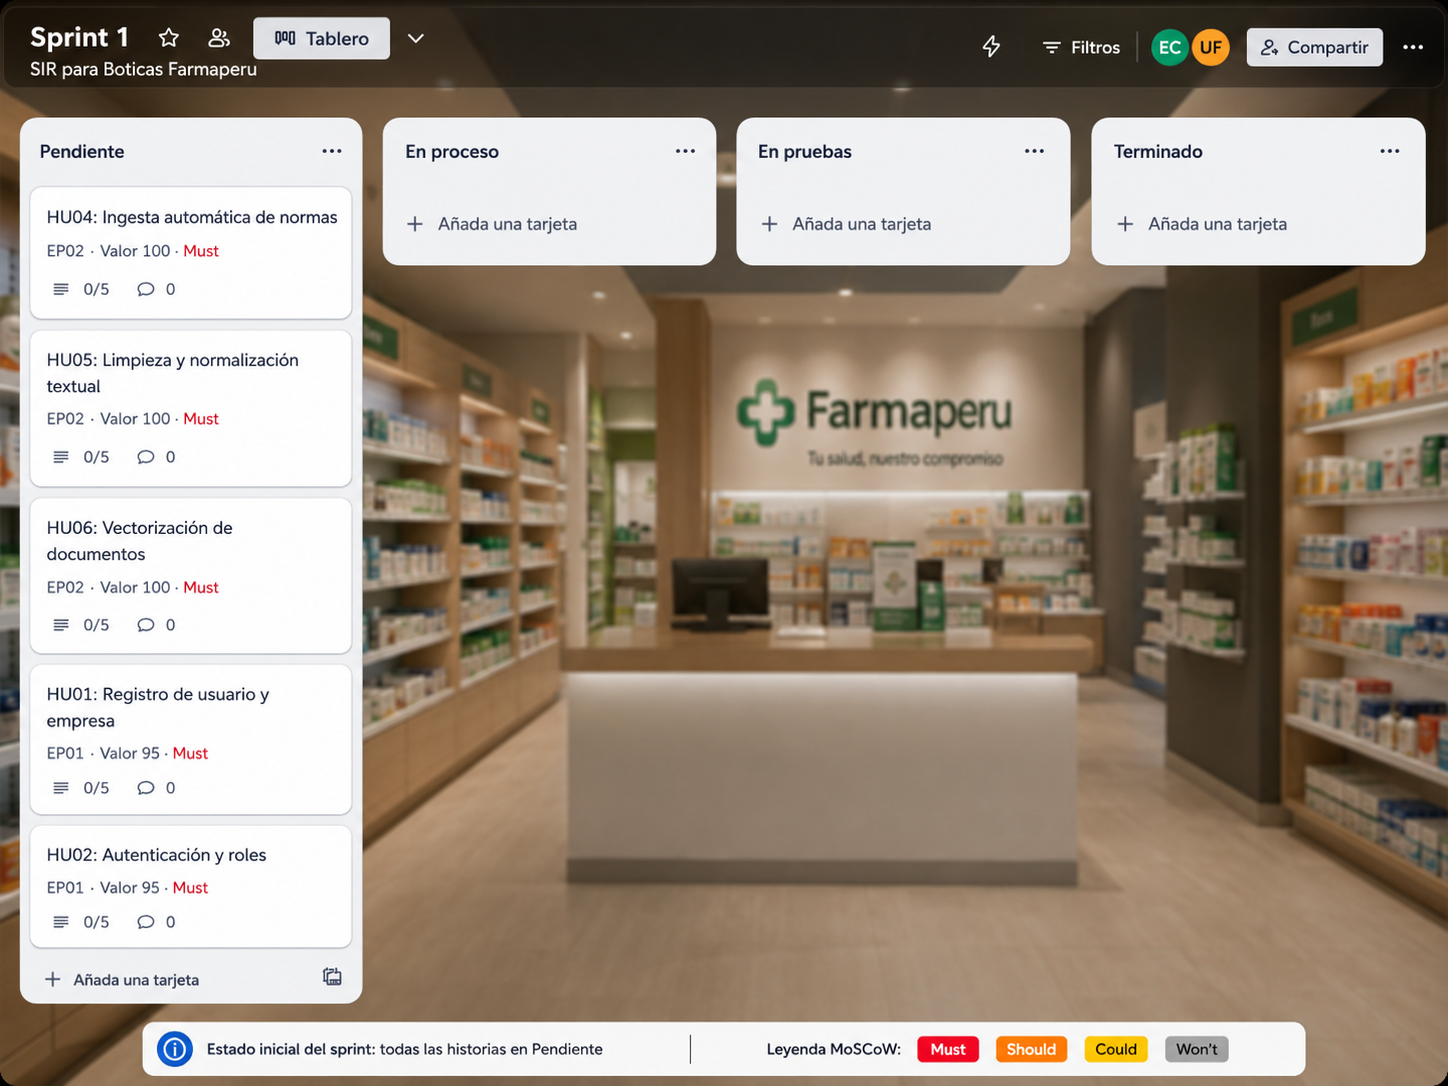
\includegraphics[width=7.5629in,height=5.67218in]{figuras/docx_image11.png}\phantomsection\label{_Toc345464139}{}

\begin{quote}
Figura 10\\
\emph{Tablero Scrum base -- Sprint 2}
\end{quote}

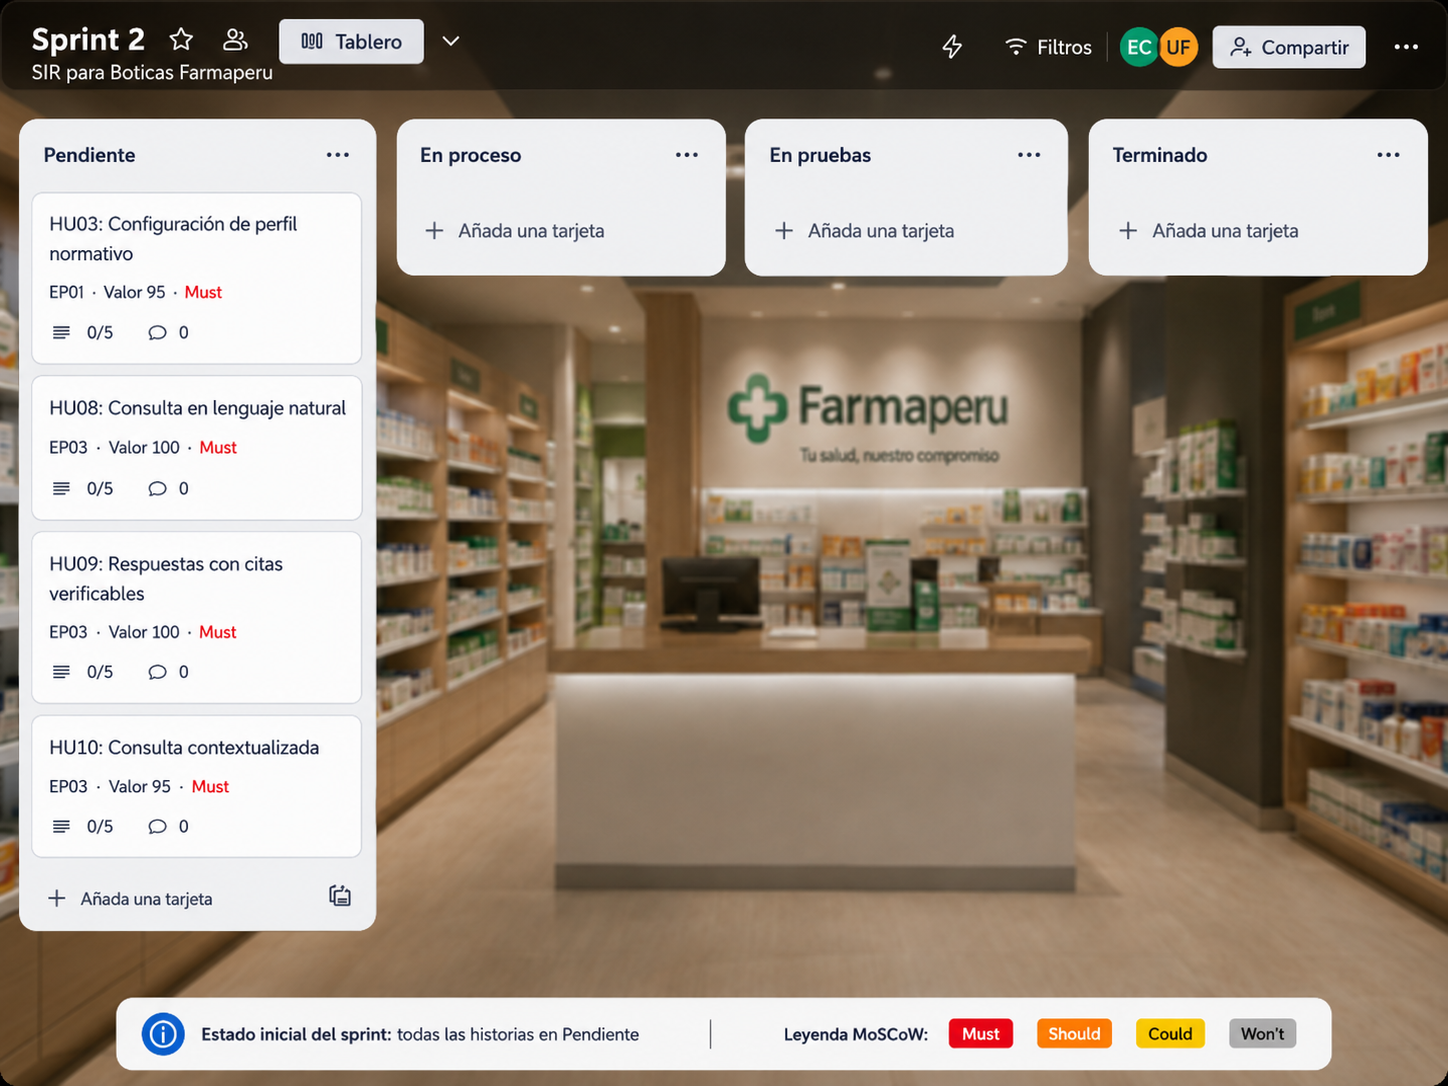
\includegraphics[width=7.58454in,height=5.6884in]{figuras/docx_image12.png}

\begin{quote}
\phantomsection\label{_Toc231672411}{}Figura 11\\
\emph{Tablero Scrum base -- Sprint 3}
\end{quote}

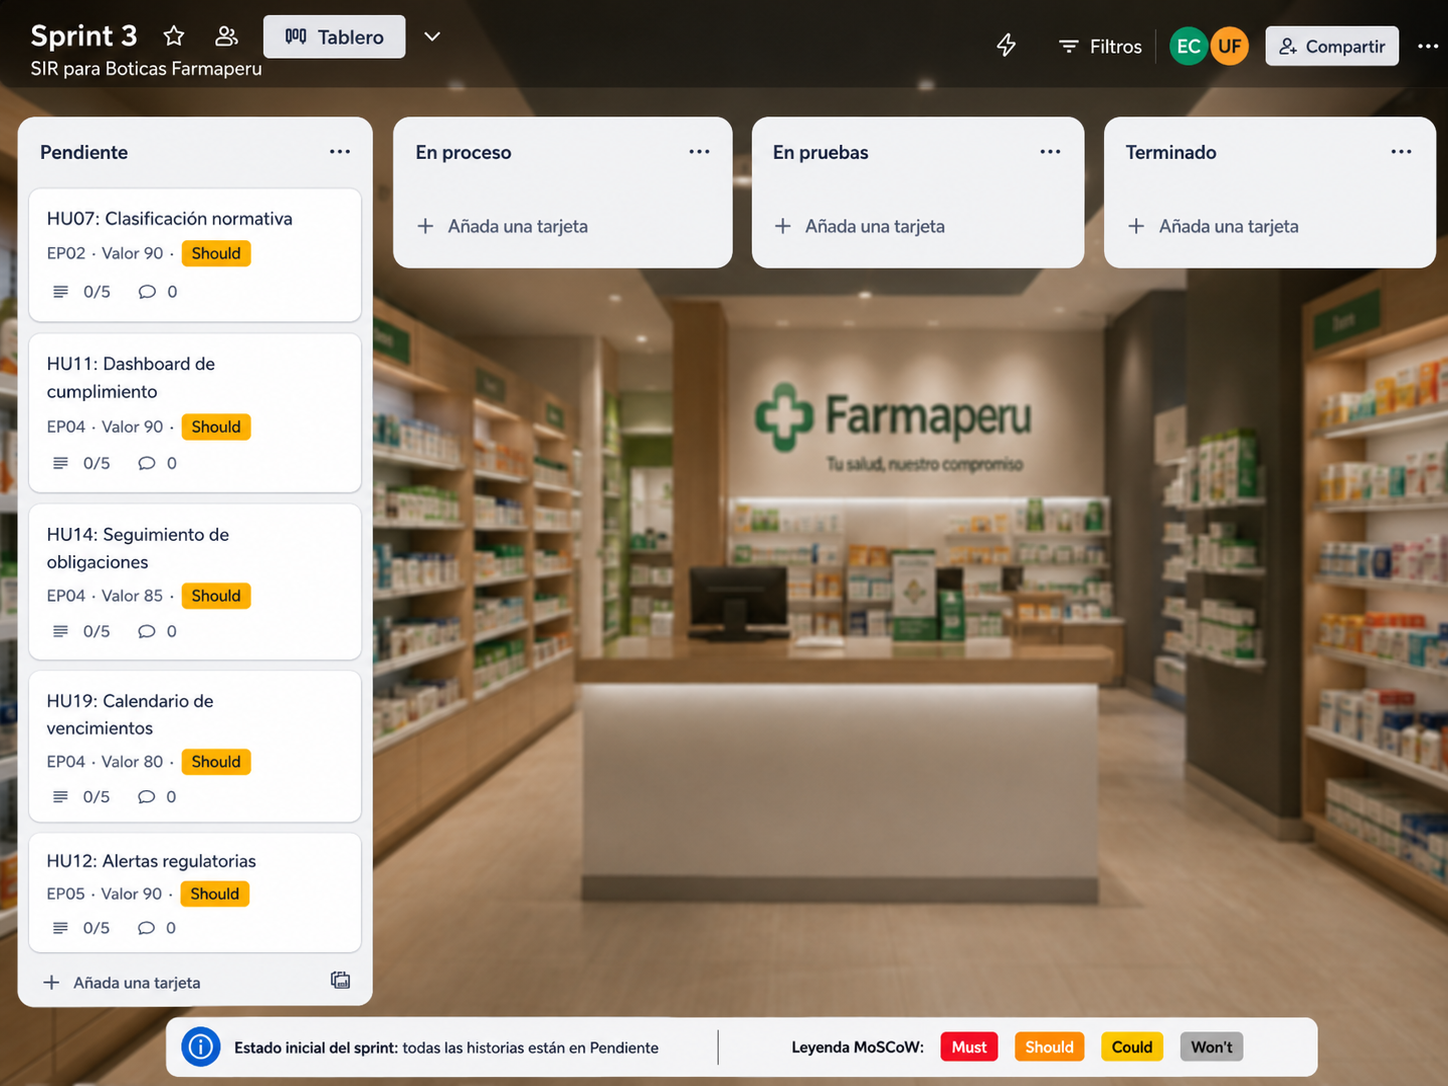
\includegraphics[width=7.65223in,height=5.73918in]{figuras/docx_image13.png}

\begin{quote}
\phantomsection\label{_Toc231672412}{}Figura 12\\
\emph{Tablero Scrum base -- Sprint 4}
\end{quote}

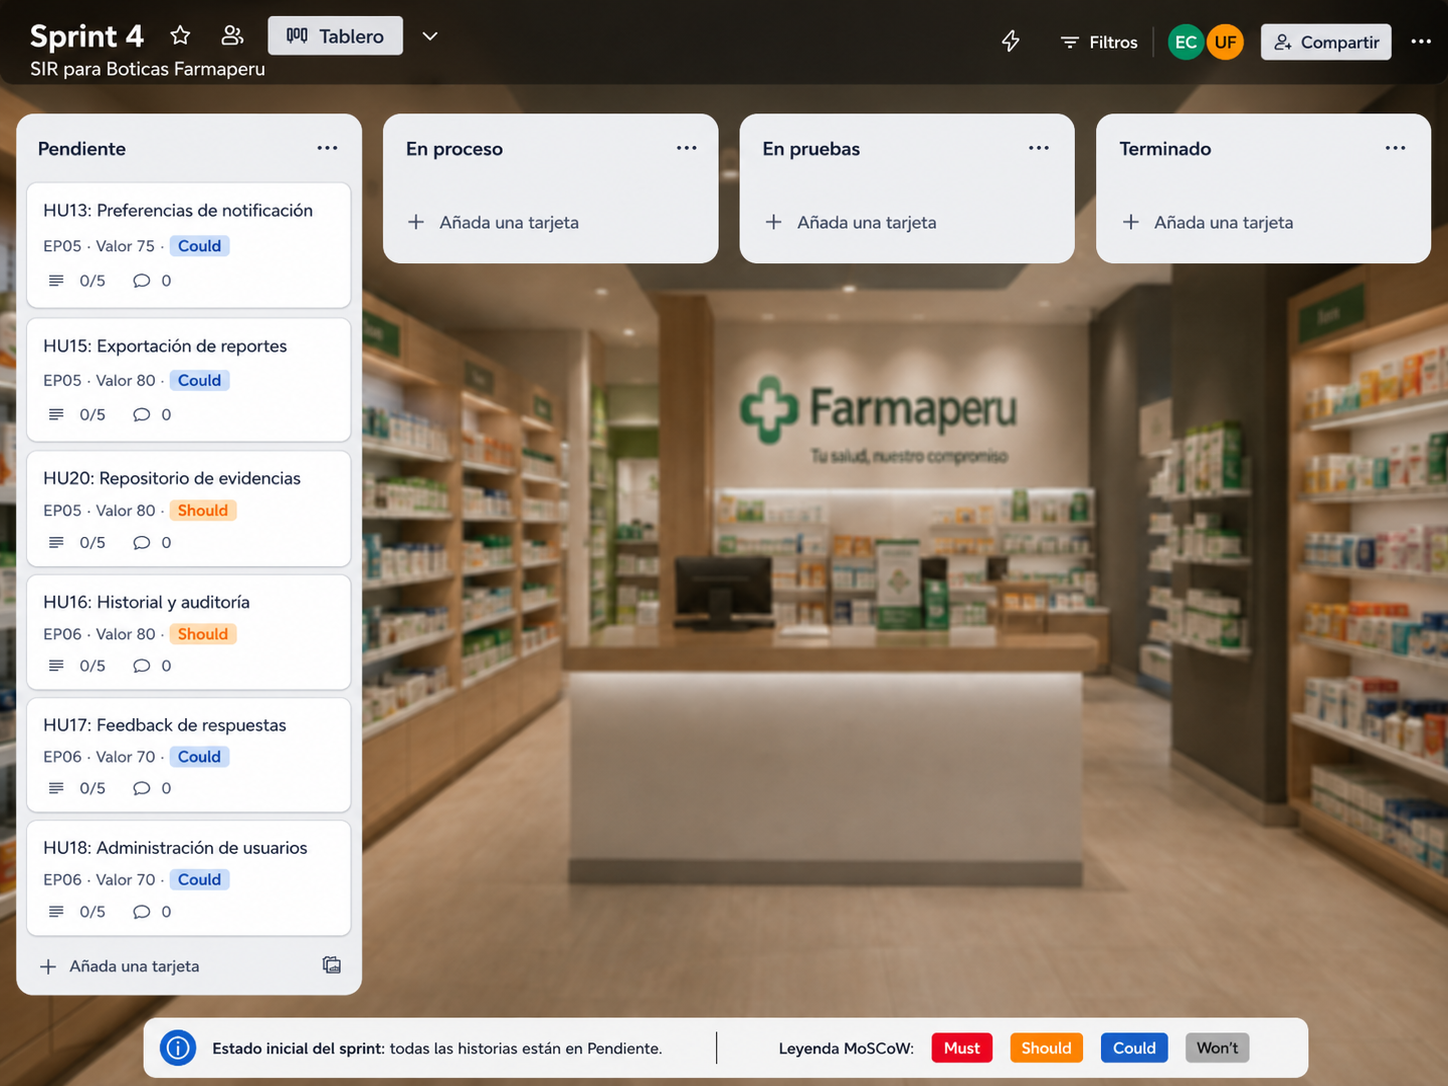
\includegraphics[width=7.57517in,height=5.68138in]{figuras/docx_image14.png}

El Product Roadmap distribuye los incrementos funcionales en cuatro
sprints. Cada sprint entrega un objetivo verificable, un conjunto de
características y métricas de aceptación. La Figura 10 presenta el
roadmap del producto.

\phantomsection\label{_Toc231672413}{}Figura 13\\
\emph{Product Roadmap}

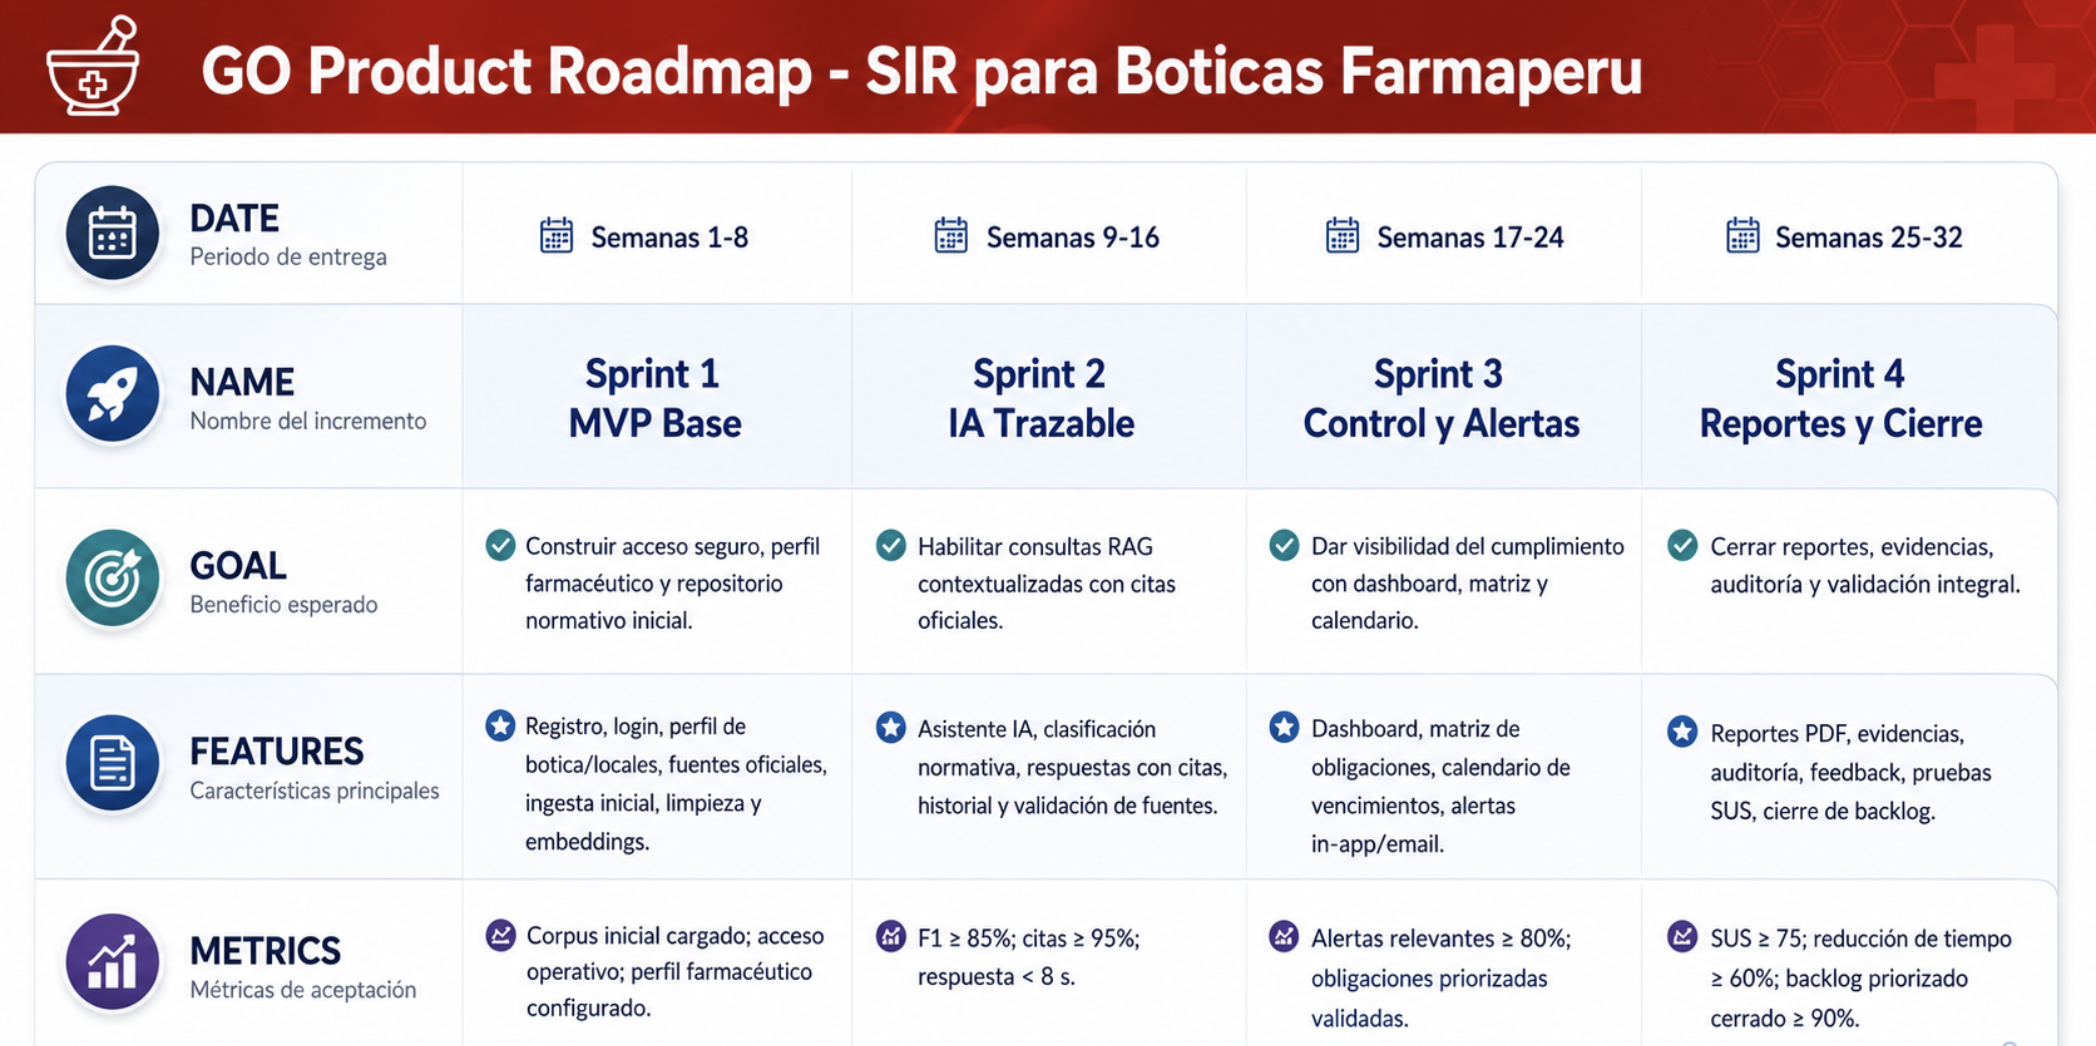
\includegraphics[width=6.5in,height=3.24375in]{figuras/docx_image15.png}

\phantomsection\label{_Toc231672278}{}Tabla 23\\
\emph{Roadmap resumido por sprint}

\begin{longtable}[]{@{}
  >{\raggedright\arraybackslash}p{(\columnwidth - 6\tabcolsep) * \real{0.1061}}
  >{\raggedright\arraybackslash}p{(\columnwidth - 6\tabcolsep) * \real{0.2877}}
  >{\raggedright\arraybackslash}p{(\columnwidth - 6\tabcolsep) * \real{0.3181}}
  >{\raggedright\arraybackslash}p{(\columnwidth - 6\tabcolsep) * \real{0.2881}}@{}}
\toprule\noalign{}
\begin{minipage}[b]{\linewidth}\raggedright
\textbf{Sprint}
\end{minipage} & \begin{minipage}[b]{\linewidth}\raggedright
\textbf{Meta}
\end{minipage} & \begin{minipage}[b]{\linewidth}\raggedright
\textbf{Características principales}
\end{minipage} & \begin{minipage}[b]{\linewidth}\raggedright
\textbf{Métrica de control}
\end{minipage} \\
\midrule\noalign{}
\endhead
\bottomrule\noalign{}
\endlastfoot
Sprint 1 & Construir el núcleo de ingesta normativa y acceso seguro. &
Registro, login, scraper inicial, limpieza textual, embeddings y
almacenamiento. & Corpus cargado y flujo de acceso operativo. \\
Sprint 2 & Habilitar consultas RAG con respuestas trazables. & Perfil
empresarial, asistente regulatorio, recuperación semántica, citaciones y
contexto del perfil. & F1 ≥ 85 \%, citas ≥ 95 \%, respuesta \textless{}
8 s. \\
Sprint 3 & Incorporar personalización, dashboard, seguimiento y alertas.
& Clasificación normativa, panel de obligaciones, calendario de
vencimientos, alertas y seguimiento. & Alertas relevantes ≥ 80 \% y
dashboard validado por usuario líder. \\
Sprint 4 & Cerrar funcionalidades complementarias y validación. &
Reportes PDF, repositorio de evidencias, historial, feedback,
administración y pruebas finales. & Validación final del sistema,
reportes generados y funcionalidades complementarias aprobadas. \\
\end{longtable}

\subsubsection{3.1.9 Otras consideraciones}\label{otras-consideraciones}

El alcance funcional del proyecto se limita a apoyar la interpretación
operativa de normas y el seguimiento de obligaciones de cumplimiento. El
SIR no emite opinión legal vinculante, no sustituye el criterio
profesional de un abogado o contador, y no ejecuta declaraciones
tributarias ni trámites ante entidades públicas.

\phantomsection\label{_Toc231672279}{}Tabla 24\\
\emph{Restricciones del proyecto}

\begin{longtable}[]{@{}
  >{\raggedright\arraybackslash}p{(\columnwidth - 2\tabcolsep) * \real{0.1923}}
  >{\raggedright\arraybackslash}p{(\columnwidth - 2\tabcolsep) * \real{0.8077}}@{}}
\toprule\noalign{}
\begin{minipage}[b]{\linewidth}\raggedright
\textbf{Restricción}
\end{minipage} & \begin{minipage}[b]{\linewidth}\raggedright
\textbf{Descripción}
\end{minipage} \\
\midrule\noalign{}
\endhead
\bottomrule\noalign{}
\endlastfoot
Restricción funcional & El sistema brinda asistencia interpretativa y
trazabilidad documental, pero no reemplaza asesoría legal, contable o
tributaria vinculante. \\
Restricción de fuentes & La calidad del resultado depende de la
disponibilidad, estructura y acceso a fuentes oficiales, comunicados y
normas públicas. \\
Restricción técnica & La precisión del motor RAG depende de la calidad
de extracción, segmentación, embeddings y prompts de generación. \\
Restricción económica & Se priorizan servicios cloud y herramientas de
bajo costo para mantener viabilidad económica en una PYME. \\
Restricción de tiempo & El desarrollo se organiza en cuatro sprints, por
lo que las funcionalidades complementarias se priorizan según valor de
negocio. \\
Restricción de seguridad & El sistema debe proteger datos de usuarios,
RUC, historial de consultas y documentos internos bajo principios de
minimización y control de acceso. \\
\end{longtable}

\subsection{3.2 Arquitectura de
software}\label{arquitectura-de-software}

La arquitectura del SIR se diseña para integrar una aplicación web, una
API de negocio, un motor de recuperación aumentada por generación, una
base de datos transaccional, una base vectorial y un proceso de ingesta
normativa. La arquitectura prioriza trazabilidad, mantenibilidad,
seguridad, escalabilidad y bajo costo operativo.

\subsubsection{3.2.1 Arquitectura Técnica
Base}\label{arquitectura-tuxe9cnica-base}

\paragraph{3.2.1.1 Diagrama conceptual}\label{diagrama-conceptual}

El diagrama conceptual muestra la relación entre los usuarios, la
aplicación web, la API del SIR, el orquestador RAG, los servicios de IA
y las fuentes normativas. Como se observa en la Figura 11, el usuario
interactúa con el sistema mediante consultas o alertas, mientras que el
backend coordina recuperación de información, generación de respuestas y
almacenamiento de evidencia.

\phantomsection\label{_Toc231672414}{}Figura 14\\
\emph{Diagrama conceptual TO-BE}

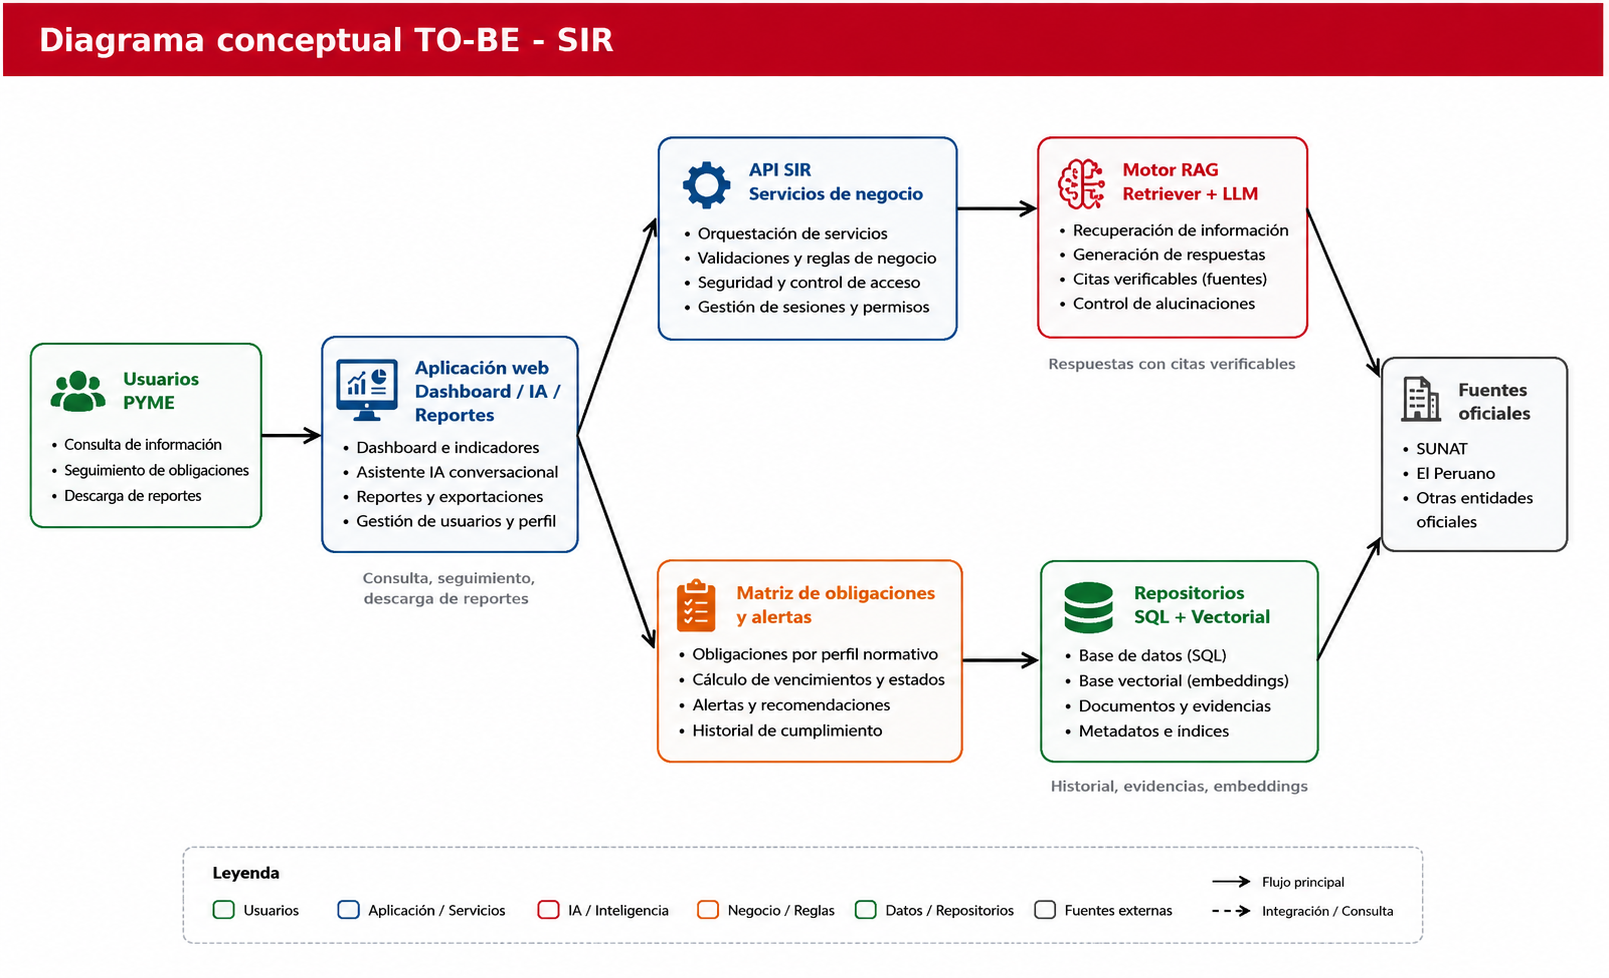
\includegraphics[width=6.5in,height=3.95347in]{figuras/docx_image16.png}

\paragraph{3.2.1.2 Diagrama físico}\label{diagrama-fuxedsico}

La arquitectura física se plantea sobre servicios cloud de bajo costo y
componentes administrados, a fin de reducir la carga operativa de
infraestructura. La Figura 12 muestra una propuesta de despliegue con
frontend en CDN, API backend, worker de ingesta, base transaccional,
base vectorial y servicios externos de IA.

\phantomsection\label{_Toc231672415}{}Figura 15\\
\emph{Arquitectura física de despliegue}

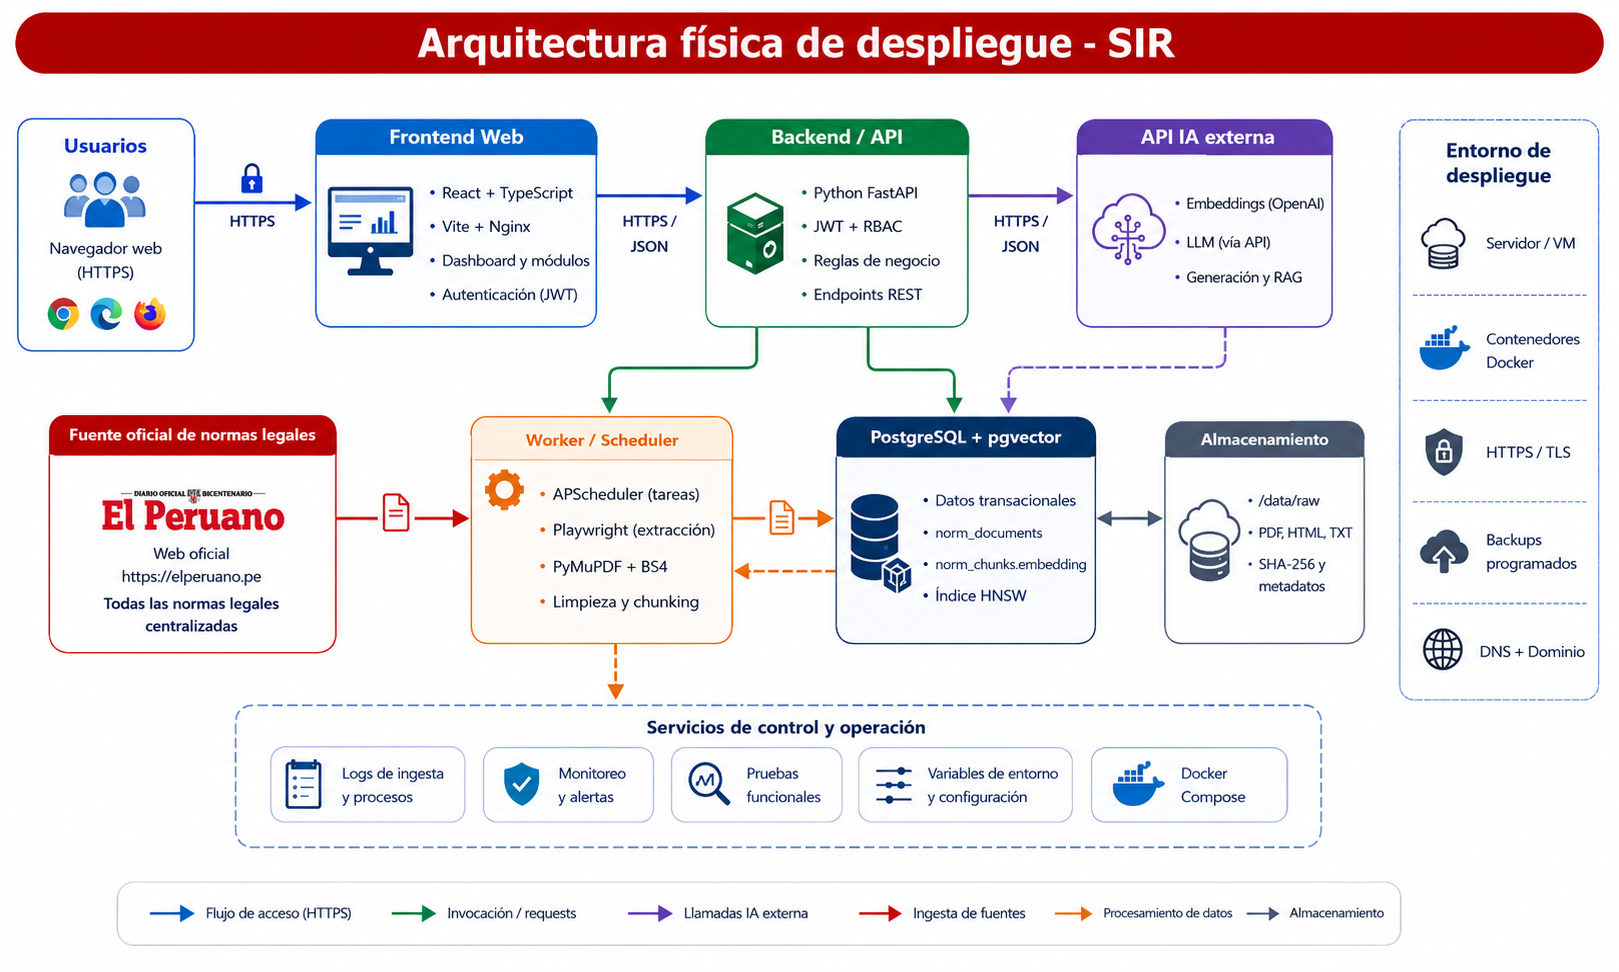
\includegraphics[width=6.5in,height=3.90486in]{figuras/docx_image17.png}

\paragraph{3.2.1.3 Diagrama lógico}\label{diagrama-luxf3gico}

El diagrama lógico organiza el sistema en capas de presentación,
aplicación, motor de IA, datos transaccionales, datos vectoriales e
ingesta normativa. Esta separación facilita la mantenibilidad, permite
escalar componentes de manera independiente y reduce el acoplamiento
entre la interfaz de usuario y los servicios de inteligencia artificial.

\phantomsection\label{_Toc231672416}{}Figura 16\\
\emph{Diagrama lógico de la solución}

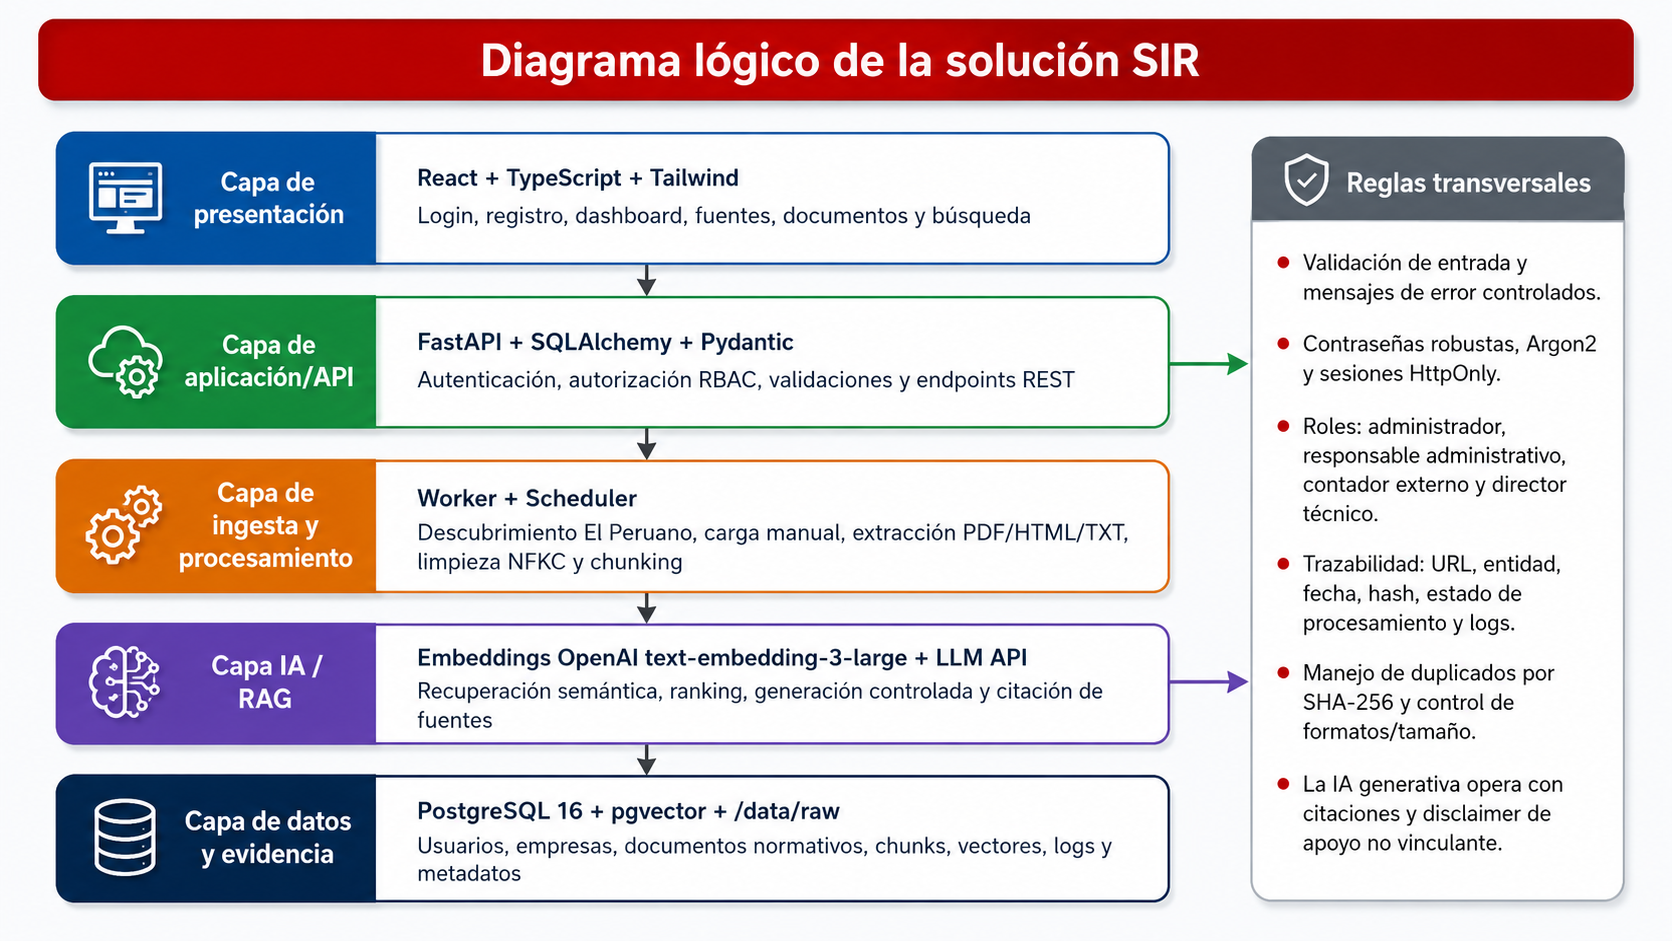
\includegraphics[width=6.5in,height=3.65417in]{figuras/docx_image18.png}

\phantomsection\label{_Toc231672280}{}Tabla 25\\
\emph{Tecnologías consideradas en la arquitectura base}

\begin{longtable}[]{@{}
  >{\raggedright\arraybackslash}p{(\columnwidth - 4\tabcolsep) * \real{0.1795}}
  >{\raggedright\arraybackslash}p{(\columnwidth - 4\tabcolsep) * \real{0.3404}}
  >{\raggedright\arraybackslash}p{(\columnwidth - 4\tabcolsep) * \real{0.4801}}@{}}
\toprule\noalign{}
\begin{minipage}[b]{\linewidth}\raggedright
\textbf{Componente}
\end{minipage} & \begin{minipage}[b]{\linewidth}\raggedright
\textbf{Tecnología}
\end{minipage} & \begin{minipage}[b]{\linewidth}\raggedright
\textbf{Justificación}
\end{minipage} \\
\midrule\noalign{}
\endhead
\bottomrule\noalign{}
\endlastfoot
Frontend & React, TypeScript, TailwindCSS, Vite y Nginx & Permite
construir una interfaz web modular, responsiva y servida como artefacto
estático dentro del contenedor frontend. \\
Backend/API & Python, FastAPI, SQLAlchemy y Pydantic & Expone servicios
REST, validación de datos, documentación automática, persistencia y
reglas de negocio del SIR. \\
Seguridad y acceso & JWT en cookie HttpOnly, Argon2/Pwdlib y RBAC &
Asegura autenticación, cierre de sesión, recuperación de contraseña,
control de permisos y segregación de funciones por rol. \\
Ingesta normativa & Worker Python, APScheduler, HTTPX,
Playwright/Chromium, PyMuPDF y BeautifulSoup & Automatiza ingesta
programada y manual, renderiza búsquedas dinámicas de El Peruano,
descarga PDF/HTML/TXT, deduplica por SHA-256 y registra logs. \\
Procesamiento textual & Normalización Unicode NFKC, limpieza legal y
segmentación por artículos/disposiciones & Convierte documentos
oficiales en fragmentos normativos trazables, preservando estructura
jurídica para recuperación semántica. \\
Embeddings & API OpenAI text-embedding-3-large, 1536 dimensiones &
Genera vectores semánticos para fragmentos normativos. En el TO-BE final
la API de embeddings es obligatoria; el fallback local solo se admite en
pruebas o desarrollo. \\
Modelo generativo & API LLM externa compatible con OpenAI & Genera
respuestas en lenguaje natural usando contexto recuperado y citas
verificables. Es componente obligatorio para completar la arquitectura
RAG final. \\
Base transaccional y vectorial & PostgreSQL 16 + pgvector, índice HNSW
de distancia coseno & Centraliza usuarios, empresas, fuentes, trabajos,
documentos, fragmentos, metadatos y embeddings, manteniendo trazabilidad
entre datos transaccionales y búsqueda semántica. \\
Almacenamiento documental & Volumen /data/raw mediante bind mount &
Conserva documentos originales descargados o cargados, permitiendo
auditoría y reprocesamiento controlado. \\
Despliegue & Docker Compose: frontend, backend, worker y postgres &
Permite ejecutar el ambiente de validación de manera reproducible, con
healthchecks y persistencia dentro del proyecto. \\
Monitoreo y pruebas & Endpoints /health y /ready, IngestionLog, pytest y
cobertura & Facilita verificación de disponibilidad, trazabilidad de
errores y validación técnica del incremento. \\
\end{longtable}

\subsubsection{3.2.2 Arquitectura Técnica
Específica}\label{arquitectura-tuxe9cnica-especuxedfica}

Para documentar la arquitectura técnica específica se utiliza el modelo
C4, porque permite representar el sistema en niveles progresivos:
contexto, contenedores y componentes. Estas vistas se complementan con
la arquitectura lógica de datos y la arquitectura física de despliegue.

\paragraph{3.2.2.1 Diagrama de contexto}\label{diagrama-de-contexto}

El diagrama de contexto identifica al SIR como sistema central y muestra
su interacción con usuarios internos y externos, así como con fuentes
regulatorias. La Figura 14 evidencia que el sistema no opera de manera
aislada, sino que se articula con entidades públicas, fuentes oficiales
y usuarios responsables de la ejecución de acciones de cumplimiento.

\phantomsection\label{_Toc231672417}{}Figura 17\\
\emph{Diagrama de contexto}

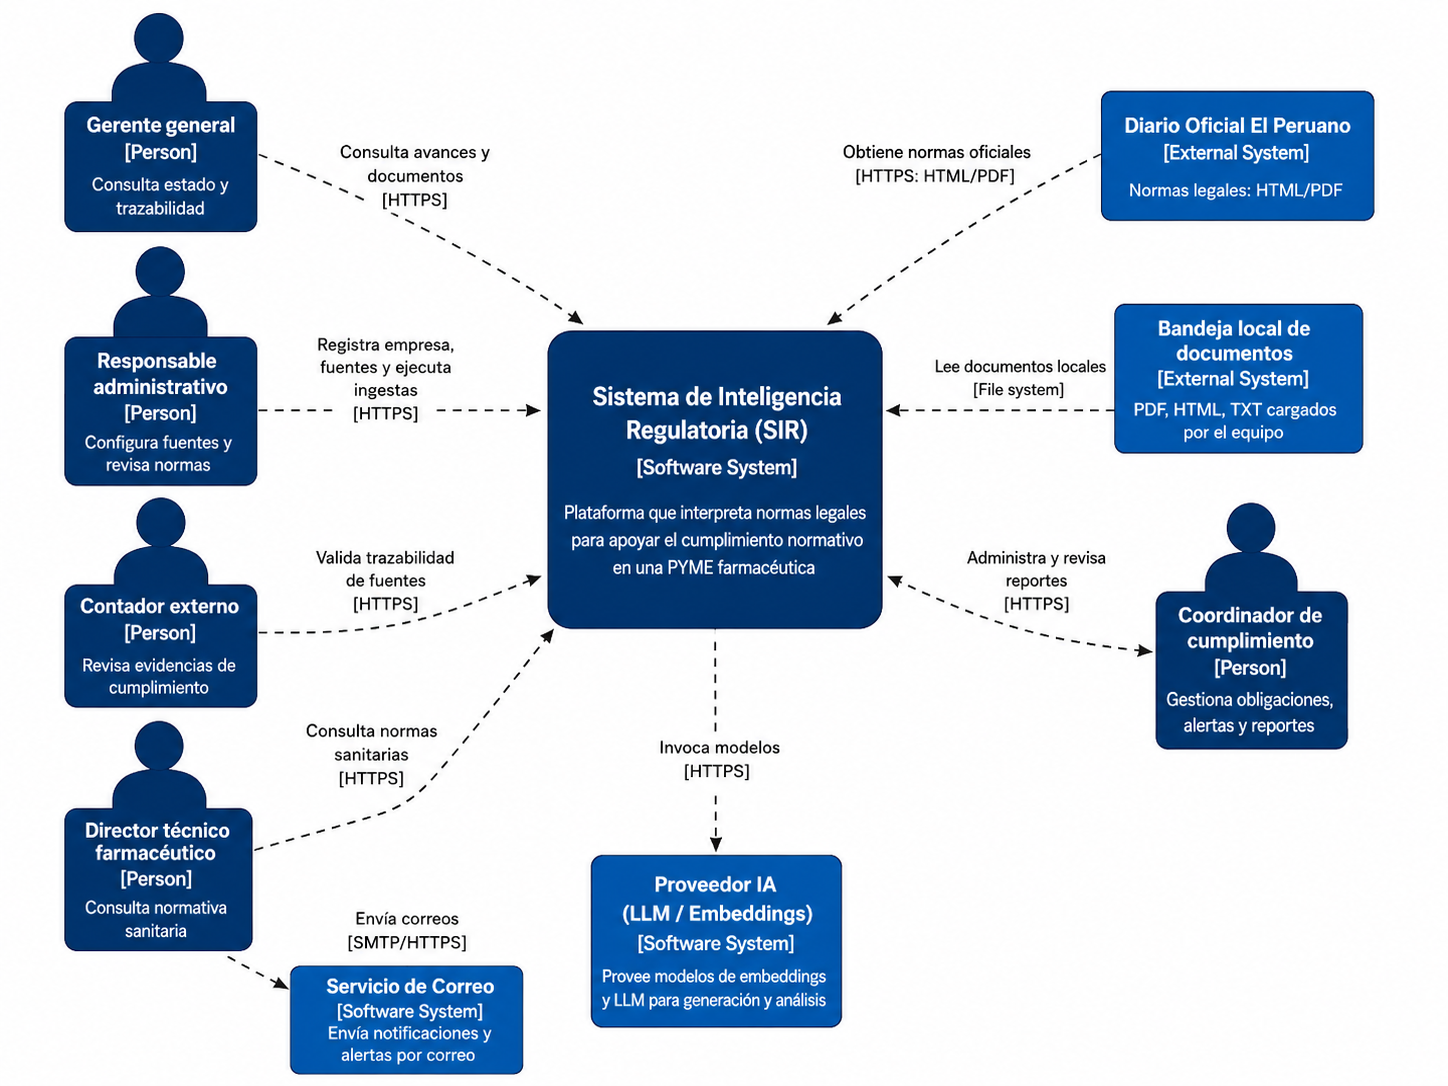
\includegraphics[width=6.5in,height=4.875in]{figuras/docx_image19.png}

\emph{Nota}. Elaboración propia, bajo el enfoque del modelo C4.

\paragraph{3.2.2.2 Diagrama de
contenedores}\label{diagrama-de-contenedores}

La vista de contenedores descompone el sistema en aplicaciones y
servicios desplegables. Como se presenta en la Figura 15, la aplicación
web se comunica con la API REST, la cual coordina el motor RAG, el
servicio de ingesta, la base transaccional, la base vectorial y el
servicio de notificaciones.

\phantomsection\label{_Toc231672418}{}Figura 18\\
\emph{Diagrama de contenedores}

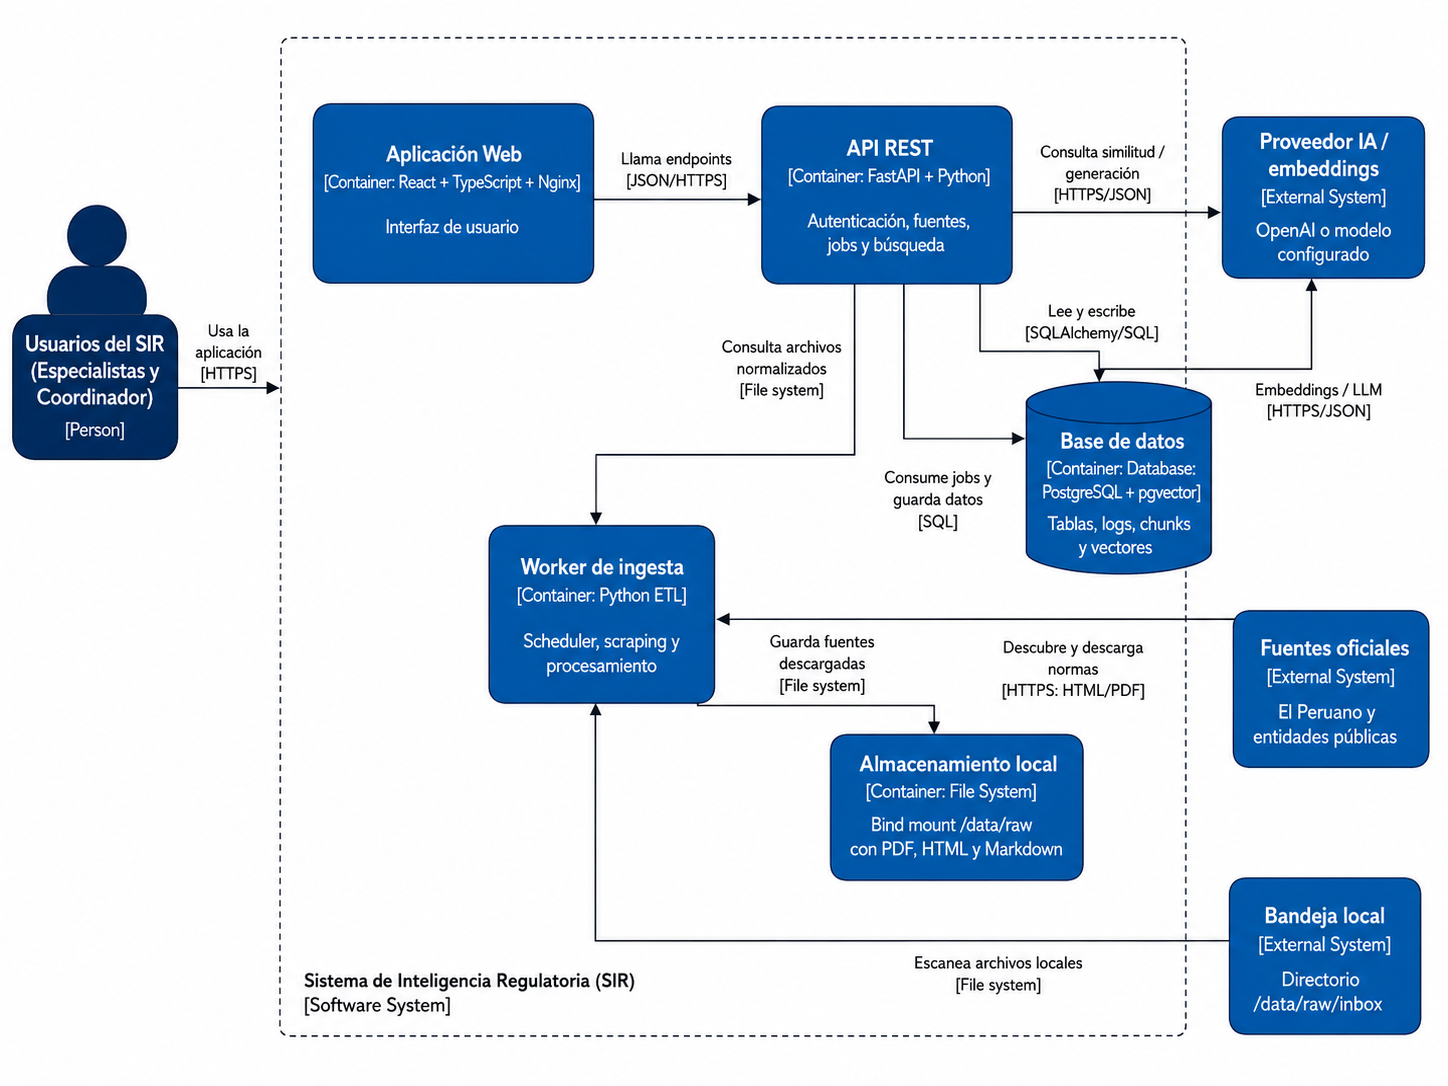
\includegraphics[width=6.5in,height=4.875in]{figuras/docx_image20.png}

\emph{Nota}. Elaboración propia, bajo el enfoque del modelo C4.

\paragraph{3.2.2.3 Diagrama de
componentes}\label{diagrama-de-componentes}

La vista de componentes detalla los módulos internos de la API y del
motor de IA. La Figura 16 muestra servicios de autenticación, perfil,
chat, alertas, reportes, orquestación RAG, recuperación semántica, capa
de citación, procesamiento ETL, clasificación normativa y planificación
de tareas.

\phantomsection\label{_Toc231672419}{}Figura 19\\
\emph{Diagrama de componentes}

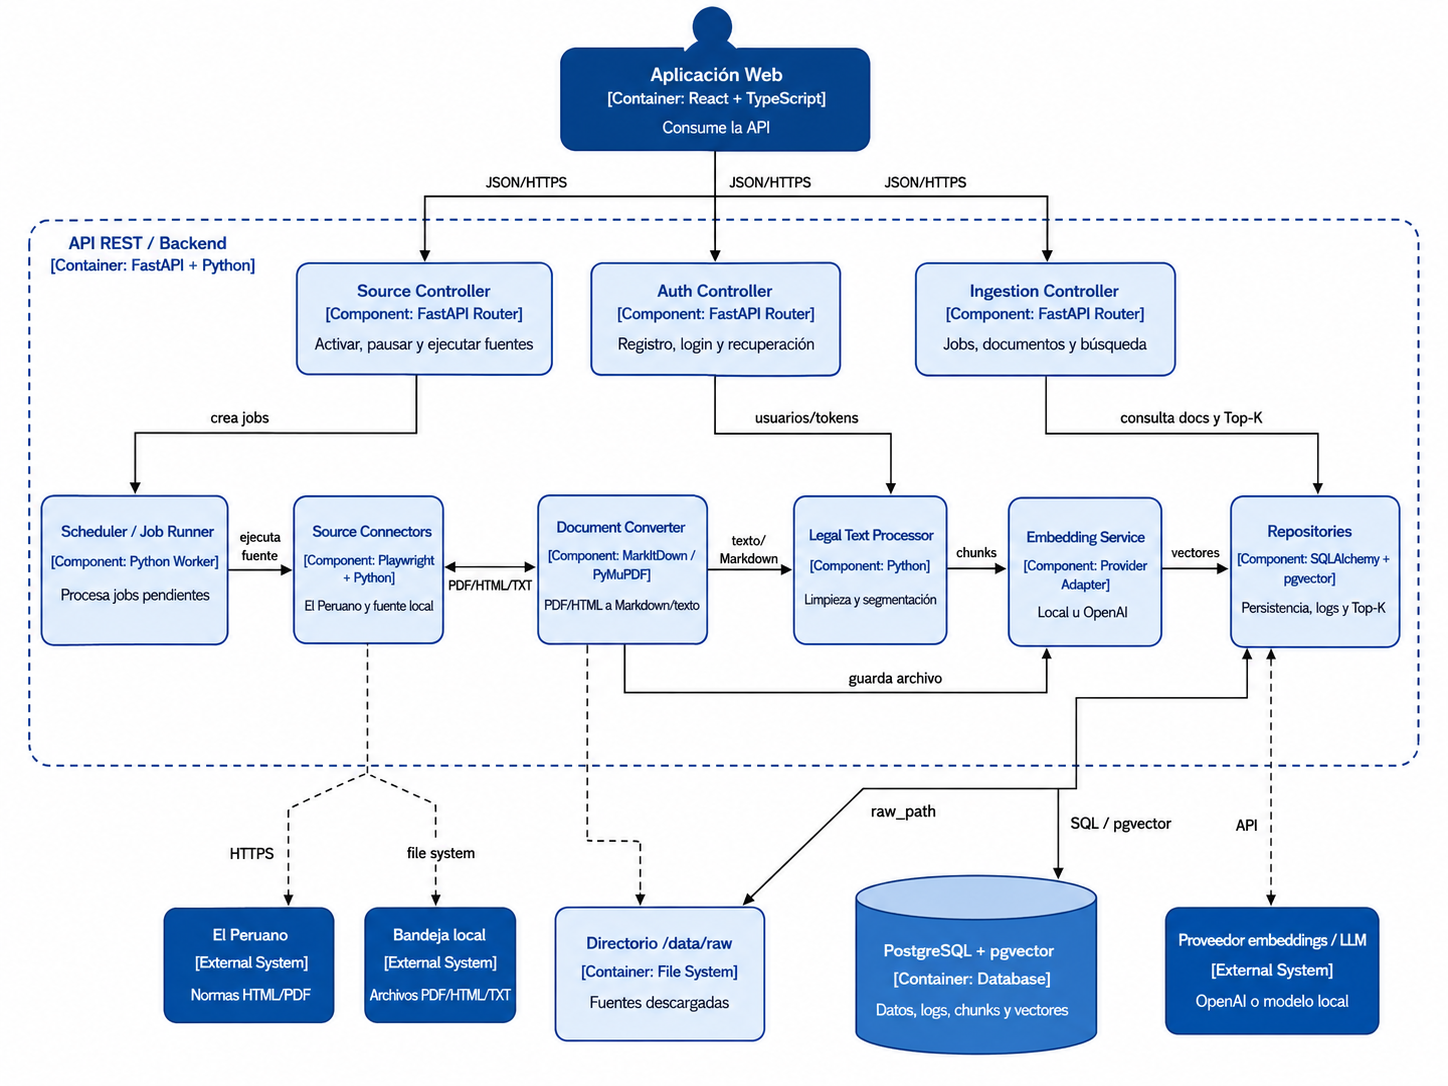
\includegraphics[width=6.5in,height=4.875in]{figuras/docx_image21.png}

\emph{Nota}. Elaboración propia, bajo el enfoque del modelo C4.

\paragraph{3.2.2.4 Arquitectura lógica de
datos}\label{arquitectura-luxf3gica-de-datos}

La arquitectura lógica de datos define las entidades principales
necesarias para soportar las funcionalidades del SIR. La Figura 17
presenta entidades relacionadas con usuarios, empresas, perfil
normativo, normas, fragmentos normativos, consultas, citaciones y
alertas. Esta estructura permite mantener trazabilidad entre una
respuesta generada y los fragmentos normativos utilizados.

\phantomsection\label{_Toc231672420}{}Figura 20\\
\emph{Arquitectura lógica de datos}

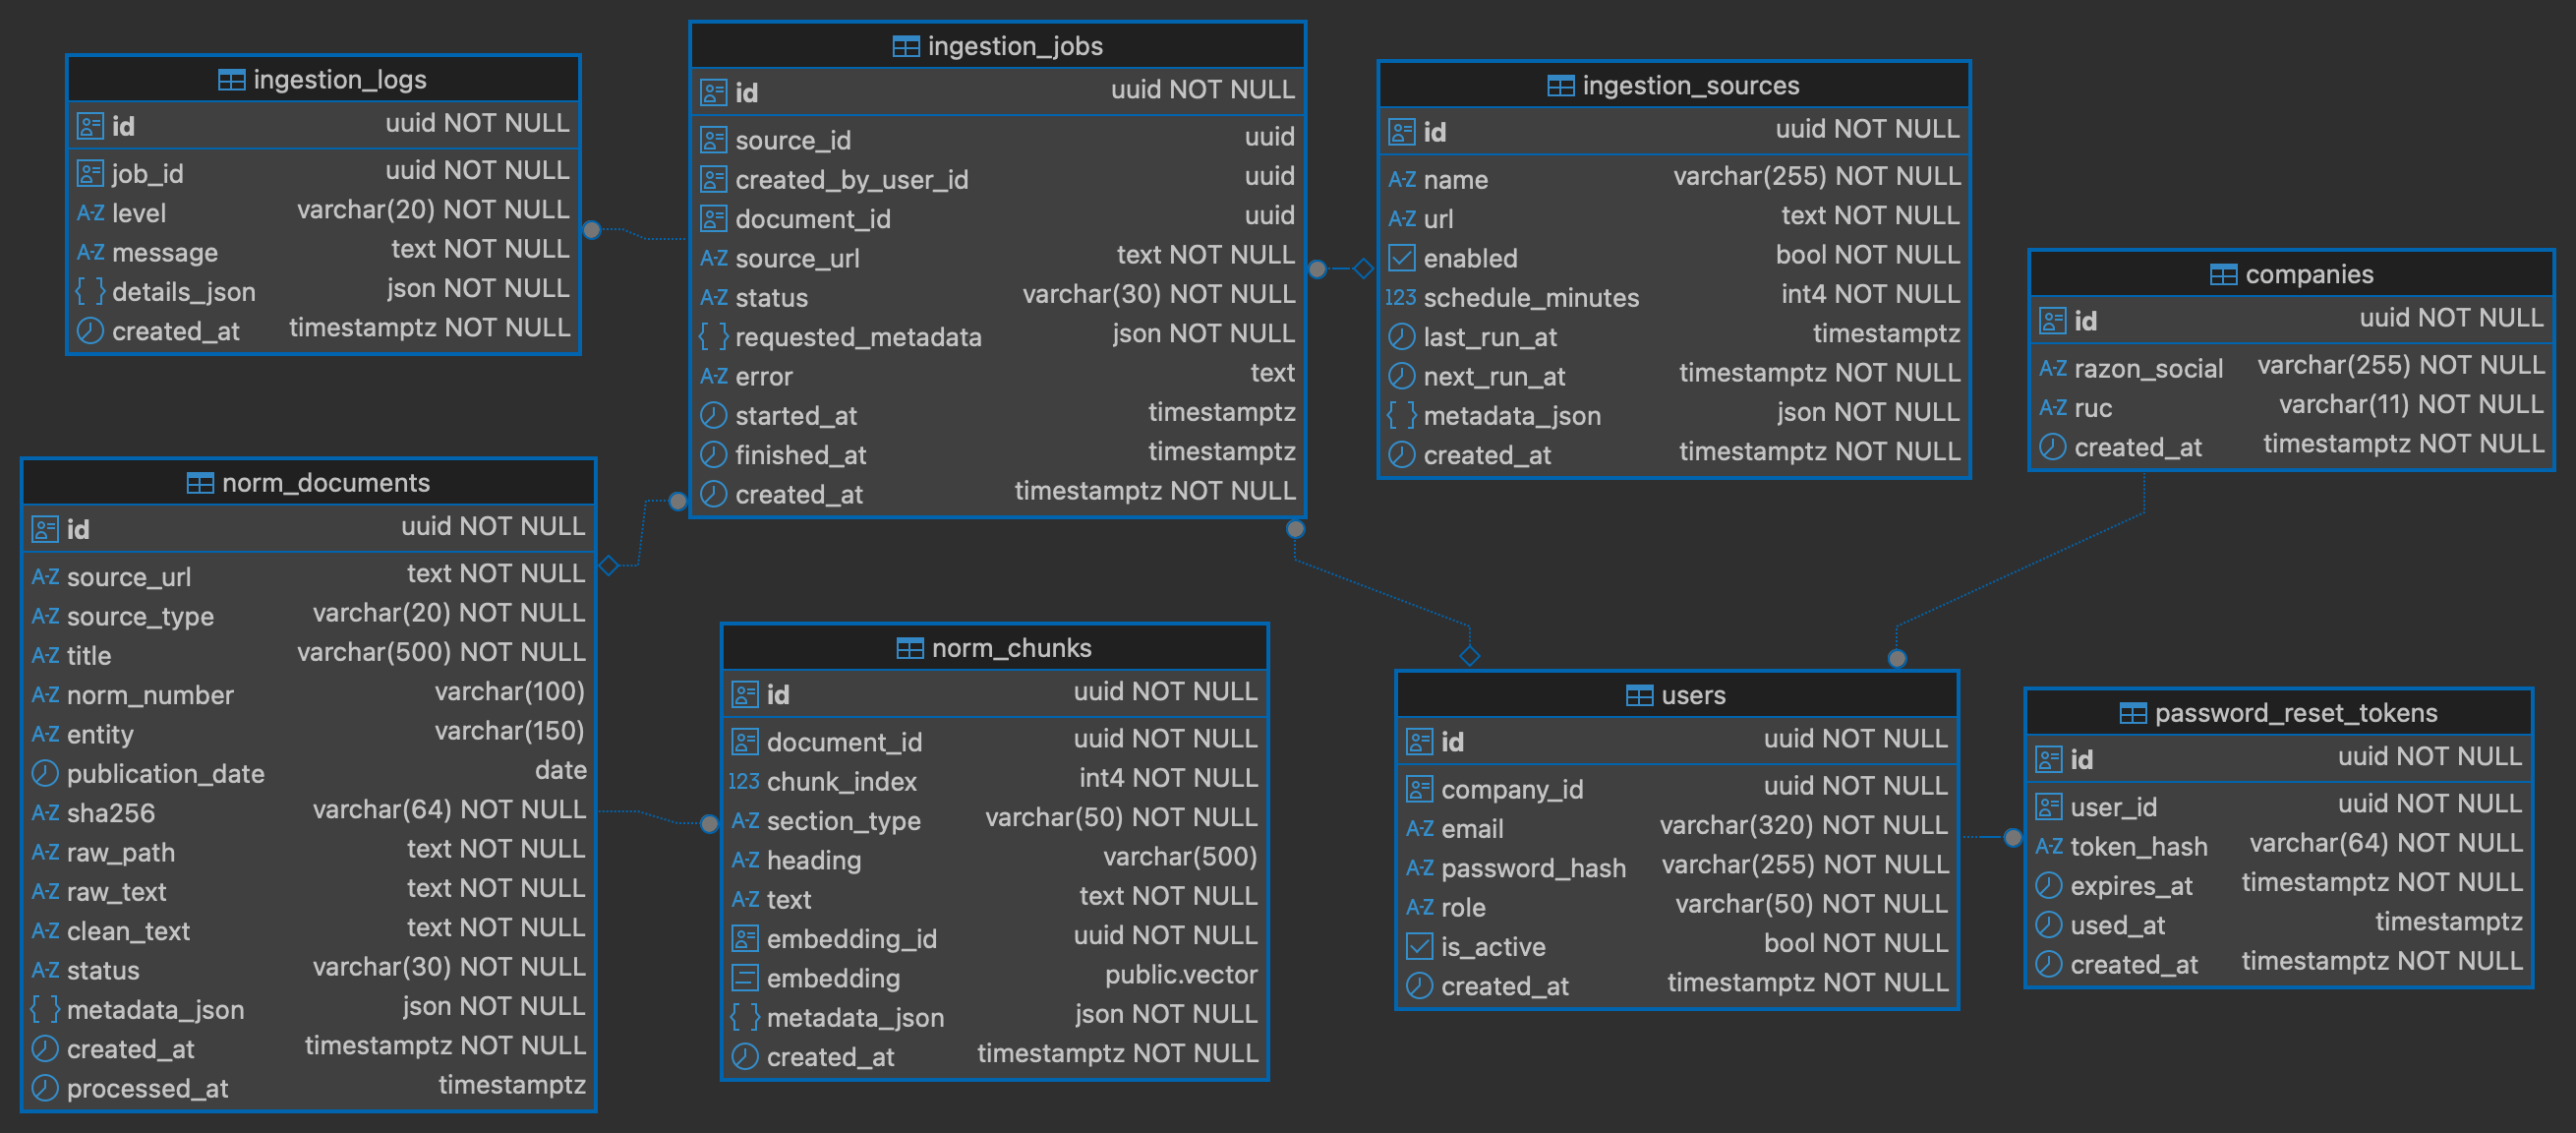
\includegraphics[width=6.5in,height=2.85833in]{figuras/docx_image22.png}

\paragraph{3.2.2.5 Atributos de calidad de
software}\label{atributos-de-calidad-de-software}

Los atributos de calidad permiten validar que la arquitectura no solo
cubra funcionalidades, sino también condiciones operativas relevantes
para una solución RegTech. La Tabla 25 define escenarios y metas
medibles para desempeño, disponibilidad, seguridad, mantenibilidad,
escalabilidad, trazabilidad y usabilidad.

\phantomsection\label{_Toc231672281}{}Tabla 26\\
\emph{Atributos de calidad de software}

\begin{longtable}[]{@{}
  >{\raggedright\arraybackslash}p{(\columnwidth - 4\tabcolsep) * \real{0.1647}}
  >{\raggedright\arraybackslash}p{(\columnwidth - 4\tabcolsep) * \real{0.4236}}
  >{\raggedright\arraybackslash}p{(\columnwidth - 4\tabcolsep) * \real{0.4116}}@{}}
\toprule\noalign{}
\begin{minipage}[b]{\linewidth}\raggedright
\textbf{Atributo}
\end{minipage} & \begin{minipage}[b]{\linewidth}\raggedright
\textbf{Escenario}
\end{minipage} & \begin{minipage}[b]{\linewidth}\raggedright
\textbf{Meta}
\end{minipage} \\
\midrule\noalign{}
\endhead
\bottomrule\noalign{}
\endlastfoot
Desempeño & El usuario realiza una consulta normativa con contexto
empresarial. & Respuesta menor a 8 segundos bajo carga normal. \\
Disponibilidad & El usuario requiere consultar obligaciones durante
horario operativo. & Disponibilidad mensual igual o superior a 99 \%. \\
Seguridad & El sistema almacena datos de usuario, RUC, historial de
consultas y evidencias. & Autenticación, control de roles, cifrado en
tránsito y hashing de contraseñas. \\
Trazabilidad & Una respuesta generada por IA debe ser verificable. & Al
menos 95 \% de respuestas con fuente oficial, fecha, entidad y fragmento
citado. \\
Mantenibilidad & El equipo debe incorporar cambios normativos o mejoras
del prompt sin afectar todo el sistema. & Componentes desacoplados,
versionamiento y despliegue controlado. \\
Escalabilidad & Aumenta el volumen de normas y consultas. & Separación
entre API, base vectorial y worker de ingesta para escalar por
componente. \\
Usabilidad & El usuario líder valida la facilidad de uso de la solución.
& SUS igual o superior a 75 puntos. \\
\end{longtable}

\paragraph{3.2.2.6 Vistas de arquitectura}\label{vistas-de-arquitectura}

La documentación arquitectónica del SIR se organiza en las siguientes
vistas:

\begin{itemize}
\item
  \textbf{Vista de contexto:} delimita el sistema, los usuarios y las
  fuentes externas.
\item
  \textbf{Vista de contenedores:} identifica aplicaciones, servicios y
  repositorios desplegables.
\item
  \textbf{Vista de componentes:} describe módulos internos de backend,
  RAG, ingesta y alertas.
\item
  \textbf{Vista de datos:} modela entidades transaccionales, fragmentos
  normativos, embeddings, consultas y citaciones.
\item
  \textbf{Vista de despliegue:} representa la infraestructura física o
  cloud requerida para operar la solución.
\end{itemize}

\paragraph{3.2.2.7 Modelo de
documentación}\label{modelo-de-documentaciuxf3n}

El modelo de documentación combina C4 para comunicar la arquitectura
desde distintos niveles de abstracción y el enfoque de atributos de
calidad para justificar decisiones técnicas. Esta combinación permite
que el diseño sea comprensible para usuarios de negocio y, al mismo
tiempo, verificable por el equipo técnico encargado de la
implementación.

\section{4. Capítulo 4: Desarrollo de la
Solución}\label{capuxedtulo-4-desarrollo-de-la-soluciuxf3n}

En este capítulo se desarrolla la implementación de los cuatro sprints
propuestos como solución del proyecto. Para ello, se organiza y
planifica el trabajo correspondiente a cada sprint, se construyen las
funcionalidades definidas, se realizan reuniones de seguimiento para
coordinar y verificar los avances, y al finalizar cada iteración se
evalúa el trabajo completado. Asimismo, se llevan a cabo retrospectivas
orientadas a la mejora continua del proceso. De igual manera, se
considera el refinamiento del backlog del producto, con el propósito de
mantenerlo actualizado y alineado con las necesidades del proyecto.

\subsection{4.1 Desarrollo de Sprint 1}\label{desarrollo-de-sprint-1}

El Sprint 1 tuvo como propósito establecer la base operativa del Sistema
de Inteligencia Regulatoria (SIR), centrando su alcance en el desarrollo
del núcleo de acceso seguro y del pipeline normativo necesario para
habilitar posteriormente la arquitectura RAG. A diferencia de los
sprints siguientes, este primer incremento no requiere la generación de
respuestas mediante OpenAI, ya que su finalidad principal es consolidar
una base verificable compuesta por usuarios, fuentes, documentos, texto
normalizado, fragmentos y representaciones semánticas. Esta decisión
técnica contribuye a disminuir los costos iniciales, mitigar los riesgos
asociados a posibles alucinaciones y conservar la flexibilidad del
sistema para integrarse con diferentes proveedores de embeddings durante
las etapas posteriores de validación.

\subsubsection{4.1.1 Sprint Planning}\label{sprint-planning}

En esta sección se presentan los principales aspectos abordados durante
la reunión de planificación del Sprint 1, desarrollada en el marco del
proyecto.

\paragraph{4.1.1.1 Definición de terminado
DoD}\label{definiciuxf3n-de-terminado-dod}

Se formalizaron los criterios mínimos para considerar una historia de
usuario como terminada:

\begin{itemize}
\item
  La funcionalidad implementada responde a la necesidad definida por el
  usuario o por el sistema.
\item
  Todos los criterios de aceptación de la historia se encuentran
  verificados mediante pruebas funcionales.
\item
  La implementación no presenta defectos críticos abiertos al cierre del
  sprint.
\item
  La documentación técnica y funcional del componente queda actualizada.
\item
  Los datos sensibles, credenciales y llaves de API se gestionan
  mediante variables de entorno.
\item
  Las fuentes normativas conservan trazabilidad mínima: entidad, fecha,
  URL o documento origen y estado de procesamiento.
\item
  El Product Owner o usuario líder brinda conformidad sobre el
  incremento presentado.
\end{itemize}

Estos criterios garantizan que la historia de usuario se haya completado
satisfactoriamente, cumpliendo con los estándares de calidad y los
requisitos acordados, lo que la convierte en una funcionalidad
finalizada.

\paragraph{4.1.1.2 Selección de historias de usuario para el sprint
1}\label{selecciuxf3n-de-historias-de-usuario-para-el-sprint-1}

Durante la reunión de planificación, el equipo de desarrollo analizó y
priorizó las historias de usuario que serían trabajadas en el Sprint 1.
Dicha selección se realizó en función del objetivo establecido para el
sprint, el cual orienta las funcionalidades principales que deben
desarrollarse dentro del periodo definido.

\phantomsection\label{_Toc231672282}{}Tabla 27\\
\emph{Historias de usuarios -- Sprint 1}

\begin{longtable}[]{@{}
  >{\raggedright\arraybackslash}p{(\columnwidth - 8\tabcolsep) * \real{0.1073}}
  >{\raggedright\arraybackslash}p{(\columnwidth - 8\tabcolsep) * \real{0.2562}}
  >{\raggedright\arraybackslash}p{(\columnwidth - 8\tabcolsep) * \real{0.1719}}
  >{\raggedright\arraybackslash}p{(\columnwidth - 8\tabcolsep) * \real{0.2371}}
  >{\raggedright\arraybackslash}p{(\columnwidth - 8\tabcolsep) * \real{0.2276}}@{}}
\toprule\noalign{}
\multirow{2}{=}{\begin{minipage}[b]{\linewidth}\raggedright
\textbf{ID de la historia}
\end{minipage}} &
\multirow{2}{=}{\begin{minipage}[b]{\linewidth}\raggedright
\textbf{Nombre de la historia}
\end{minipage}} &
\multicolumn{3}{>{\raggedright\arraybackslash}p{(\columnwidth - 8\tabcolsep) * \real{0.6365} + 4\tabcolsep}@{}}{%
\begin{minipage}[b]{\linewidth}\raggedright
\textbf{Descripción de la historia de usuario}
\end{minipage}} \\
& & \begin{minipage}[b]{\linewidth}\raggedright
\textbf{Como}
\end{minipage} & \begin{minipage}[b]{\linewidth}\raggedright
\textbf{Necesito}
\end{minipage} & \begin{minipage}[b]{\linewidth}\raggedright
\textbf{Para}
\end{minipage} \\
\midrule\noalign{}
\endhead
\bottomrule\noalign{}
\endlastfoot
HU01 & Registro de usuario y empresa & Responsable administrativo &
registrar mi usuario y los datos basicos de la empresa & acceder al SIR
y vincular el perfil empresarial a Boticas Farmaperu. \\
HU02 & Autenticacion y roles & Usuario registrado & iniciar sesion de
forma segura y cerrar sesion & acceder solo a las funciones
autorizadas. \\
HU04 & Ingesta automatica de normas & Sistema & extraer normas oficiales
desde El Peruano y fuentes locales & mantener actualizado el corpus
normativo con trazabilidad. \\
HU05 & Limpieza y normalizacion textual & Sistema & convertir PDF/HTML a
texto normalizado o Markdown & preparar documentos legales para
recuperacion semantica. \\
HU06 & Vectorizacion de documentos & Sistema & generar o preparar
embeddings de fragmentos normativos & habilitar busqueda semantica con
pgvector y proveedor configurable. \\
\end{longtable}

\paragraph{4.1.1.3 Validación de estimación realizada en el Inception
Agile}\label{validaciuxf3n-de-estimaciuxf3n-realizada-en-el-inception-agile}

Durante la ejecución del primer Sprint, se aplicó la técnica de Planning
Poker para evaluar y puntuar cada Historia de Usuario (HU). Este proceso
permitió contrastar y validar las proyecciones iniciales de complejidad
y esfuerzo definidas en el Inception. Para este ciclo, se seleccionaron
las siguientes cinco historias de usuario:

\textbf{\hfill\break
}

\textbf{\ul{HU01: Registro de usuario y empresa}}

Puntos de la historia: 3

\phantomsection\label{_Toc231672421}{}Figura 21\\
\emph{Votación de la HU01}

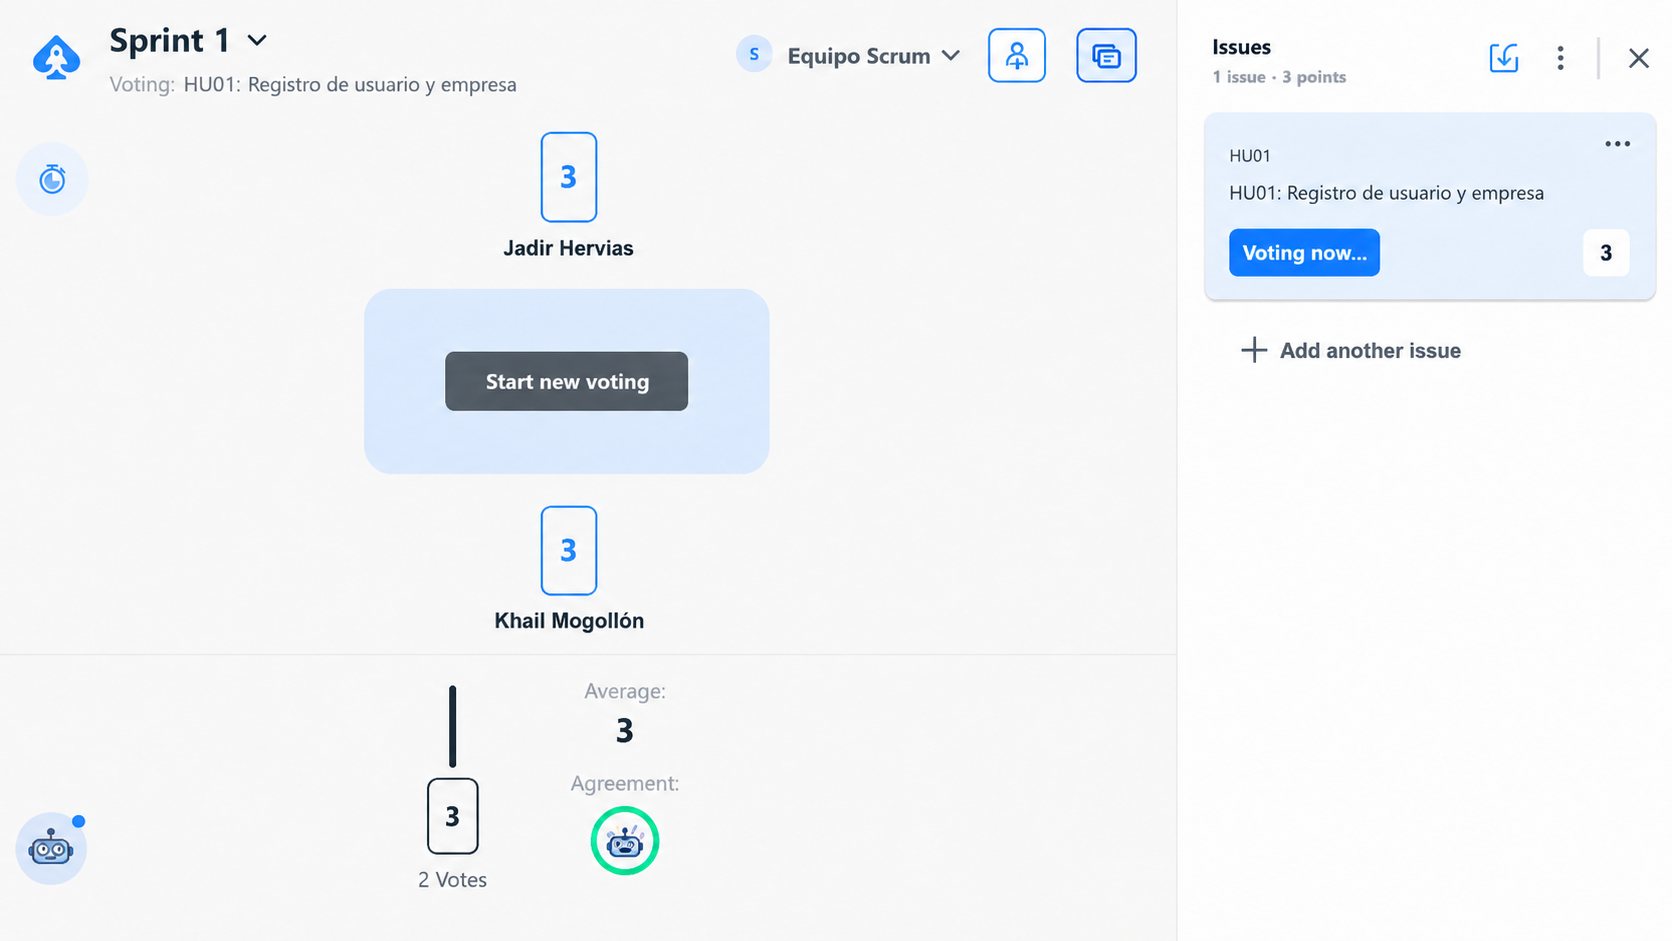
\includegraphics[width=5.02716in,height=2.82617in]{figuras/docx_image23.png}

\textbf{\ul{HU02: Autenticacion y roles}}

Puntos de la historia: 3

\phantomsection\label{_Toc231672422}{}Figura 22\\
\emph{Votación de la HU02}

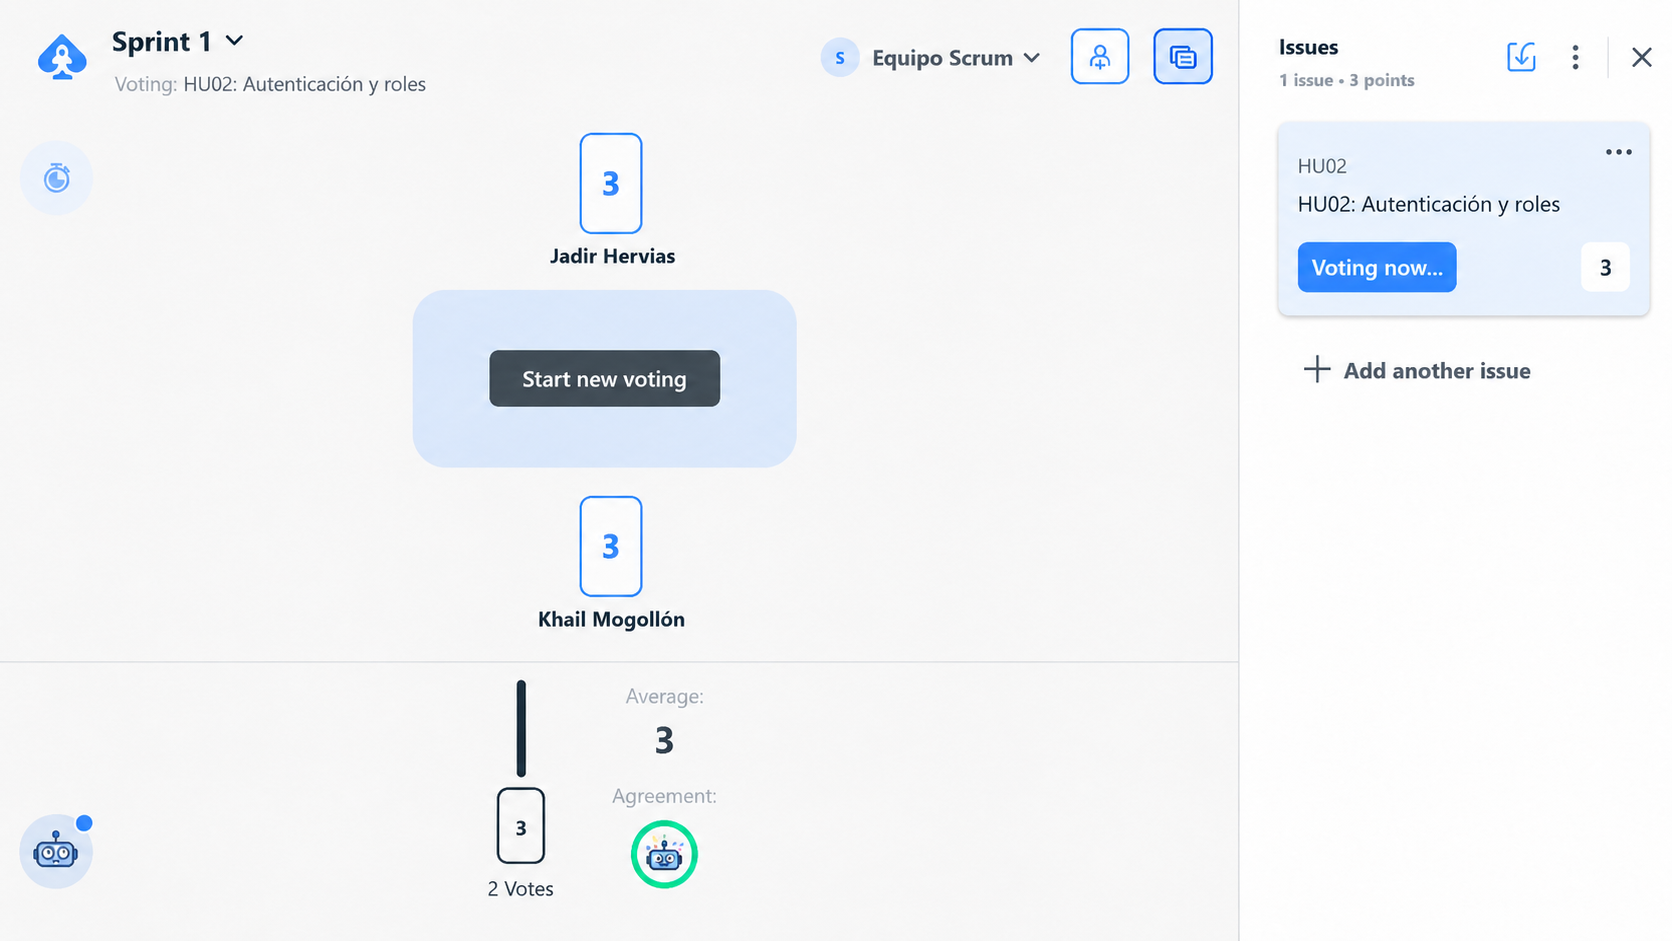
\includegraphics[width=5.20206in,height=2.92449in]{figuras/docx_image24.png}

\textbf{\ul{HU04: Ingesta automática de normas}}

Puntos de la historia: 8

\phantomsection\label{_Toc231672423}{}Figura 23\\
\emph{Votación de la HU04}

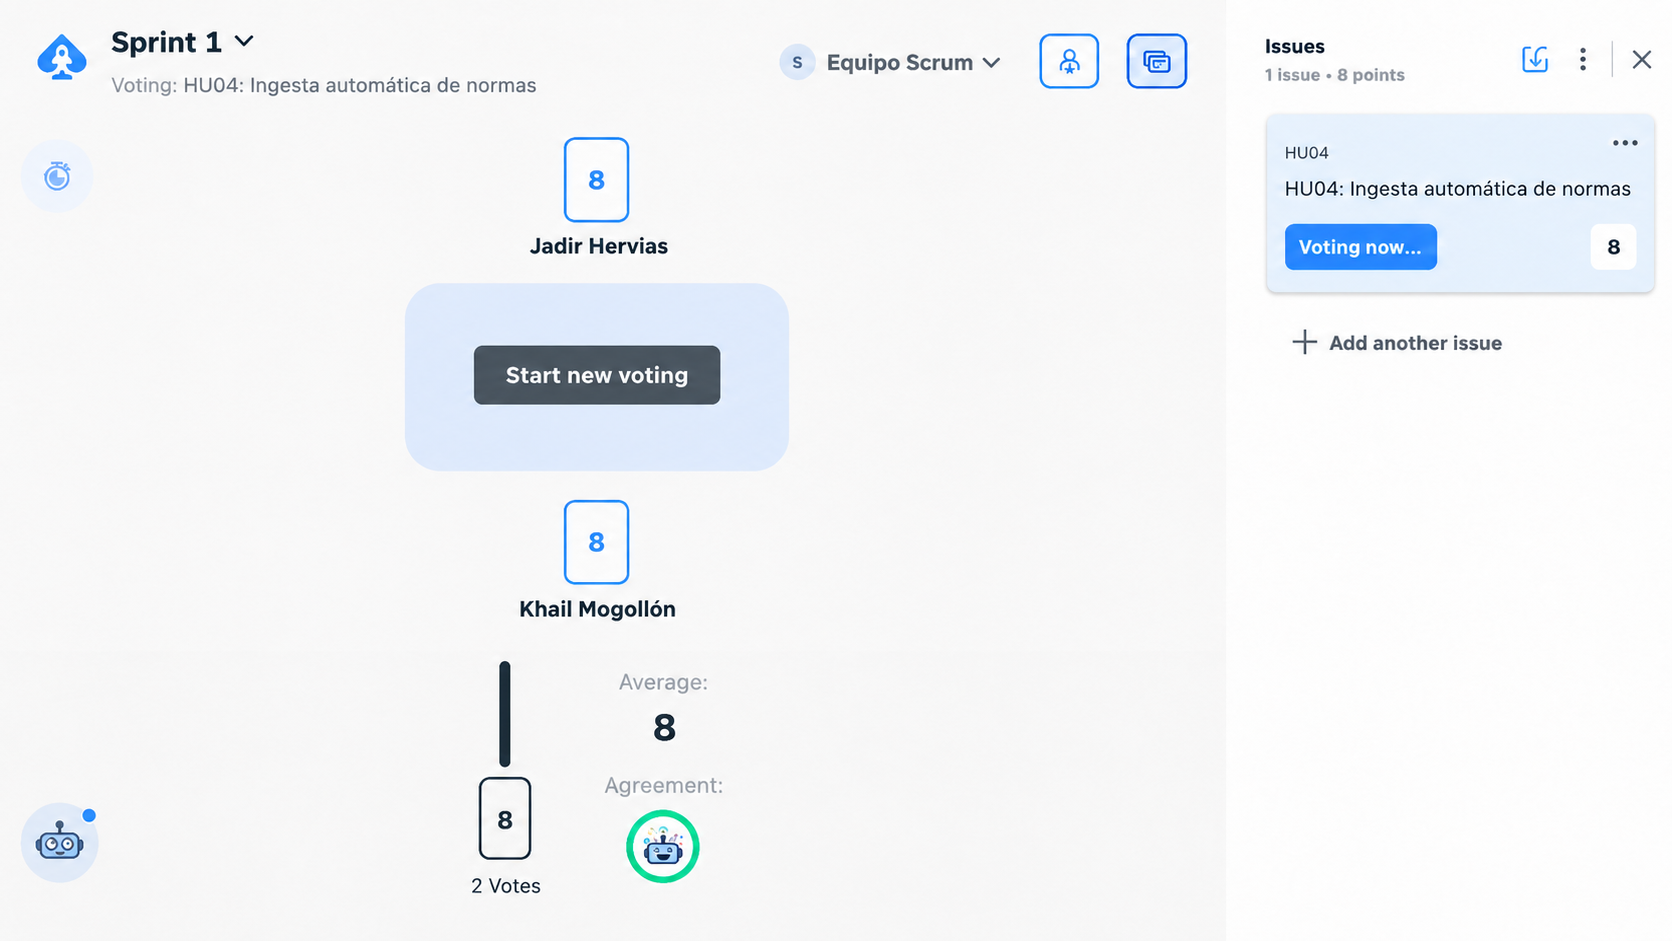
\includegraphics[width=5.13336in,height=2.88587in]{figuras/docx_image25.png}

\textbf{\ul{HU05: Limpieza y normalización textual}}

Puntos de la historia: 5

\phantomsection\label{_Toc231672424}{}Figura 24\\
\emph{Votación de la HU05}

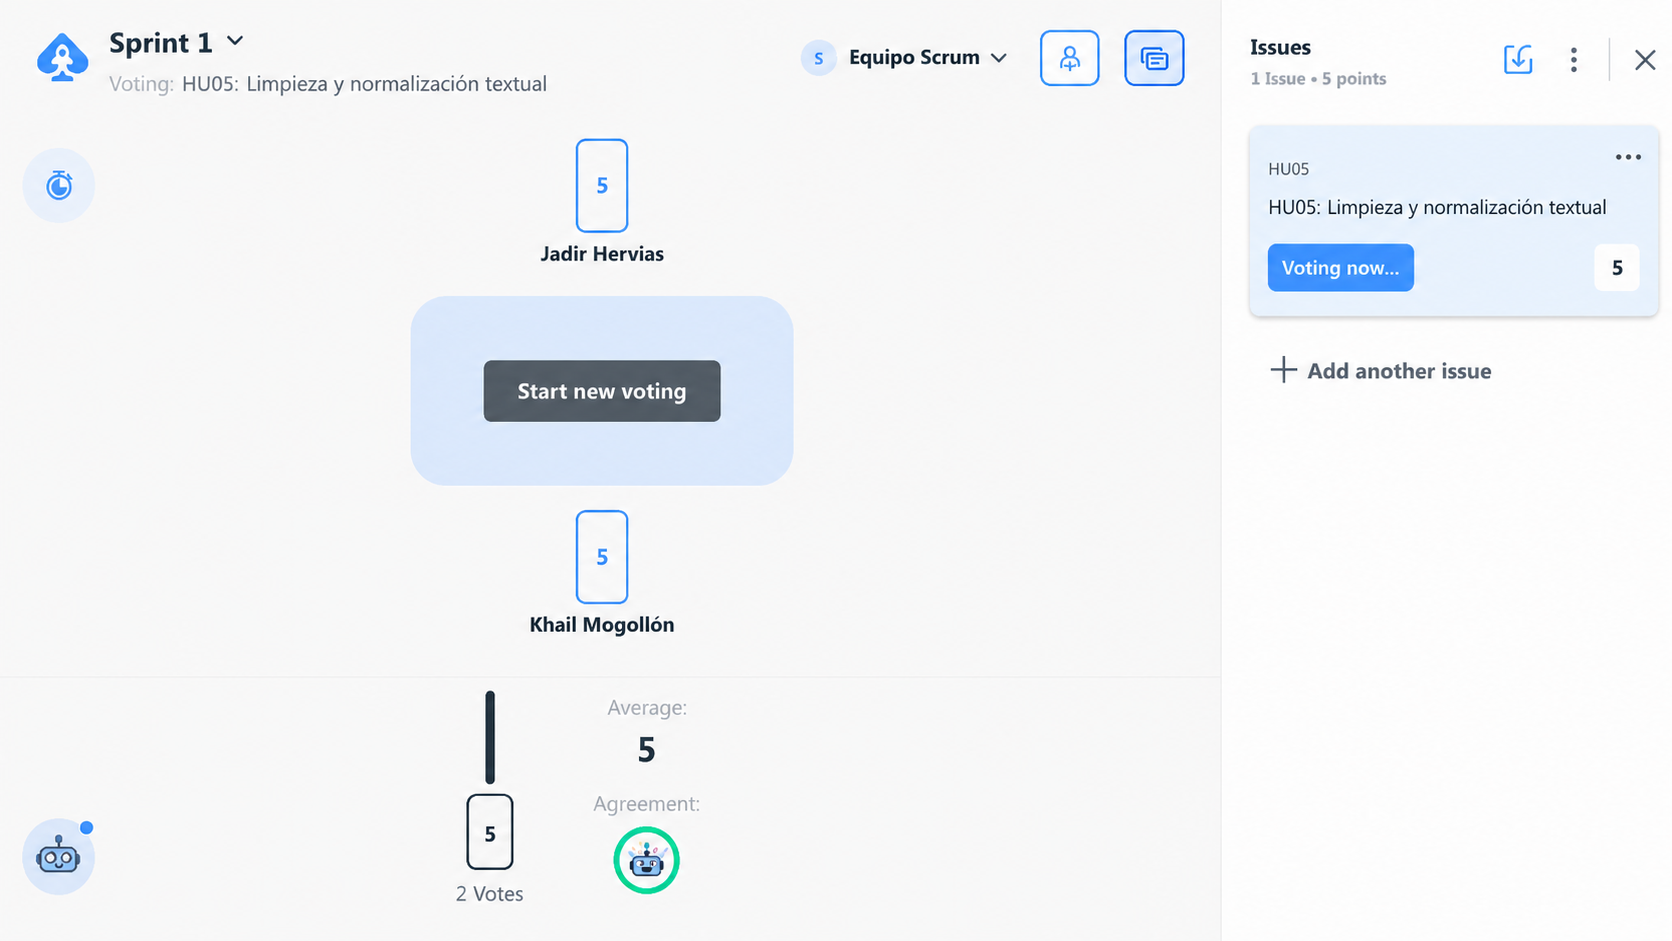
\includegraphics[width=5.16207in,height=2.90201in]{figuras/docx_image26.png}

\textbf{\ul{HU06: Vectorización de documentos}}

Puntos de la historia: 5

\phantomsection\label{_Toc231672425}{}Figura 25\\
\emph{Votación de la HU06}

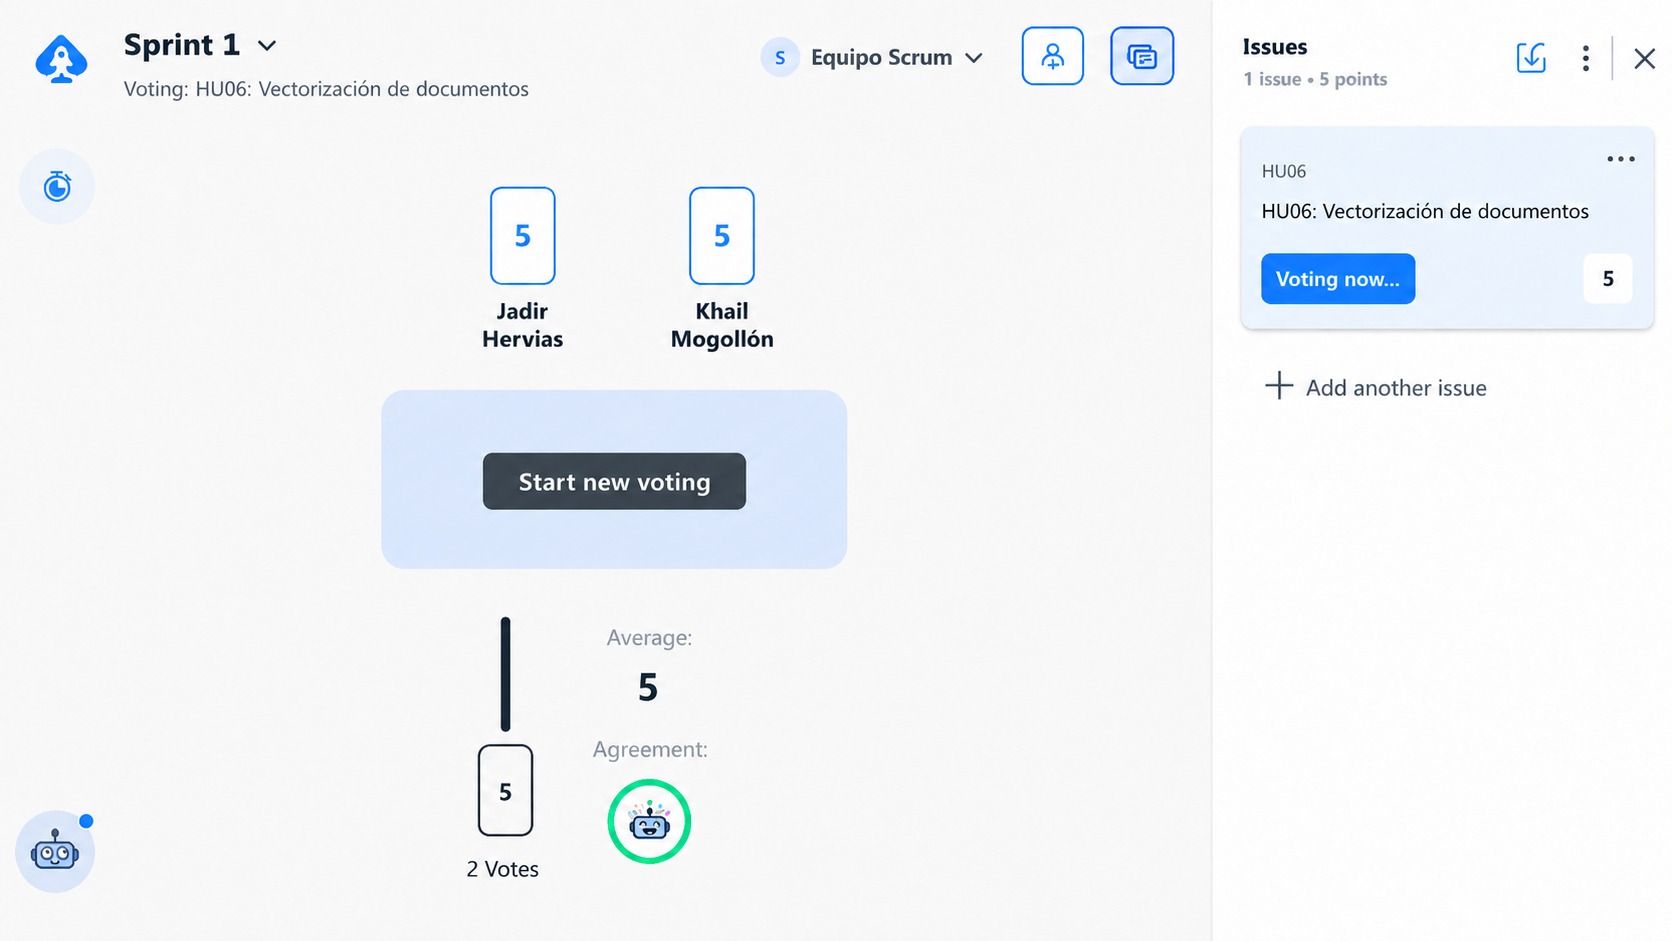
\includegraphics[width=5.42766in,height=3.05132in]{figuras/docx_image27.png}

\paragraph{4.1.1.4 Actualización de los criterios de aceptación de las
historias de
usuario}\label{actualizaciuxf3n-de-los-criterios-de-aceptaciuxf3n-de-las-historias-de-usuario}

\phantomsection\label{_Toc231672283}{}Tabla 28\\
\emph{Criterios de aceptación - Sprint 1}

\begin{longtable}[]{@{}
  >{\raggedright\arraybackslash}p{(\columnwidth - 4\tabcolsep) * \real{0.0603}}
  >{\raggedright\arraybackslash}p{(\columnwidth - 4\tabcolsep) * \real{0.1206}}
  >{\raggedright\arraybackslash}p{(\columnwidth - 4\tabcolsep) * \real{0.8191}}@{}}
\toprule\noalign{}
\begin{minipage}[b]{\linewidth}\raggedright
\textbf{ID}
\end{minipage} & \begin{minipage}[b]{\linewidth}\raggedright
\textbf{Historia de Usuario}
\end{minipage} & \begin{minipage}[b]{\linewidth}\raggedright
\textbf{Criterios de Aceptación}
\end{minipage} \\
\midrule\noalign{}
\endhead
\bottomrule\noalign{}
\endlastfoot
HU01 & Registro de usuario y empresa &
\begin{minipage}[t]{\linewidth}\raggedright
\begin{itemize}
\item
  El formulario debe permitir ingresar nombres, apellidos, correo,
  contraseña, confirmación de contraseña, razón social, nombre
  comercial, RUC, rubro, distrito, régimen tributario y número de
  trabajadores.
\item
  El sistema debe validar que los campos obligatorios no estén vacíos
  antes de enviar el registro.
\item
  El correo debe tener formato válido y no debe encontrarse previamente
  registrado en la base de datos.
\item
  El RUC debe aceptar exactamente 11 dígitos numéricos y no debe
  duplicarse para una misma empresa.
\item
  La contraseña debe tener longitud mínima de 8 caracteres y coincidir
  con el campo de confirmación.
\item
  El sistema debe crear un identificador interno para el usuario y otro
  para la empresa, asociando ambos registros.
\item
  La contraseña debe almacenarse cifrada mediante hash seguro y nunca
  debe mostrarse en texto plano.
\item
  El usuario creado debe recibir por defecto el rol Responsable
  administrativo, salvo que el administrador seleccione otro rol
  permitido.
\item
  Después de hacer clic en Registrar, debe mostrarse un mensaje de
  confirmación: ¿Estás seguro de registrar el usuario y la empresa?, con
  los botones Cancelar y Confirmar.
\item
  Si el usuario elige Cancelar en la confirmación, la operación se anula
  y los datos no se guardan.
\item
  Si el usuario elige Confirmar, el sistema guarda los datos, registra
  la fecha de alta y muestra el mensaje: Se registró correctamente.
\item
  Después de aceptar el mensaje de éxito, el sistema debe redirigir al
  usuario a la pantalla de inicio de sesión.
\end{itemize}
\end{minipage} \\
HU02 & Autenticacion y roles &
\begin{minipage}[t]{\linewidth}\raggedright
\begin{itemize}
\item
  La pantalla de inicio de sesión debe solicitar correo y contraseña, y
  validar que ambos campos sean obligatorios.
\end{itemize}

\begin{itemize}
\item
  El sistema debe autenticar al usuario comparando la contraseña
  ingresada contra el hash almacenado.
\item
  Ante credenciales incorrectas, debe mostrarse un mensaje genérico:
  Usuario o contraseña incorrectos, sin revelar cuál campo falló.
\item
  El sistema debe generar una sesión segura o token JWT con tiempo de
  expiración definido.
\item
  El sistema debe registrar la fecha y hora del último inicio de sesión
  exitoso.
\item
  El menú y las rutas deben mostrarse de acuerdo con el rol asignado al
  usuario.
\item
  Un usuario sin sesión activa no debe acceder a rutas protegidas del
  SIR.
\item
  El usuario debe poder cerrar sesión y, al hacerlo, el sistema debe
  invalidar la sesión o eliminar el token local.
\item
  Si el token expira, el sistema debe solicitar un nuevo inicio de
  sesión.
\item
  Las credenciales, tokens y variables secretas no deben quedar escritas
  en el código fuente ni en repositorios públicos.
\item
  Debe existir al menos una prueba que verifique acceso permitido y otra
  que verifique acceso denegado por rol.
\end{itemize}
\end{minipage} \\
HU04 & Ingesta automatica de normas &
\begin{minipage}[t]{\linewidth}\raggedright
\begin{itemize}
\item
  El sistema debe permitir ejecutar la ingesta normativa de forma manual
  indicando un rango de fechas.
\item
  El sistema debe quedar preparado para ejecución programada diaria
  mediante cron o tarea equivalente.
\item
  Debe existir una configuración de fuentes que permita activar o
  desactivar El Peruano y fuentes locales sin modificar el código
  fuente.
\item
  El proceso debe consultar la fuente oficial, identificar documentos
  disponibles y registrar el número de elementos descubiertos.
\item
  Cada documento descargado debe registrar metadatos mínimos: entidad,
  título, fecha de publicación, URL de origen, tipo de documento,
  checksum y estado de procesamiento.
\item
  El sistema debe almacenar el archivo original o referencia persistente
  para asegurar trazabilidad documental.
\item
  Debe evitar duplicados usando URL, fecha, título y/o checksum del
  documento.
\item
  Debe crear un registro de ingestion\_log con items\_discovered,
  jobs\_created, items\_skipped, errores, fecha de ejecución y duración
  aproximada.
\item
  Si la fuente no devuelve resultados, el sistema debe registrar
  items\_discovered = 0 sin considerarlo error automático.
\item
  Si ocurre un error de conexión, descarga o lectura, el sistema debe
  marcar el trabajo como error y conservar el mensaje técnico para
  auditoría.
\item
  La ingesta del Sprint 1 no debe depender de OpenAI ni de un modelo
  generativo, porque su objetivo es preparar el corpus verificable.
\end{itemize}
\end{minipage} \\
HU05 & Limpieza y normalizacion textual &
\begin{minipage}[t]{\linewidth}\raggedright
\begin{itemize}
\item
  El sistema debe procesar documentos con estado descargado o disponible
  para convertirlos a texto normalizado.
\item
  Debe soportar extracción desde PDF y HTML, y dejar preparado el uso de
  MarkItDown para conversión a Markdown cuando aplique.
\item
  Debe remover encabezados, pies de página, saltos excesivos, caracteres
  no válidos, espacios duplicados y cortes de palabra por salto de
  línea.
\item
  Debe conservar información legal relevante como número de norma,
  artículos, disposiciones, fechas, entidad emisora y URL oficial.
\item
  El texto normalizado debe almacenarse vinculado al documento original
  mediante document\_id.
\item
  Debe generarse una versión en Markdown o texto estructurado cuando la
  fuente lo permita.
\item
  El sistema debe dividir el documento en fragmentos manejables,
  respetando límites de tamaño y solapamiento definidos para
  recuperación semántica.
\item
  Cada fragmento debe registrar metadatos: document\_id, chunk\_id,
  orden, título o sección, fuente, fecha y estado.
\item
  Debe validar documentos vacíos o ilegibles y marcarlos como error de
  normalización.
\item
  Debe registrar logs de limpieza con conteo de caracteres, número de
  fragmentos generados y estado final.
\item
  La limpieza no debe alterar el sentido normativo del texto ni eliminar
  referencias necesarias para la citación posterior.
\end{itemize}
\end{minipage} \\
HU06 & Vectorizacion de documentos &
\begin{minipage}[t]{\linewidth}\raggedright
\begin{itemize}
\item
  El sistema debe seleccionar únicamente fragmentos normalizados y
  aprobados para vectorización.
\item
  Debe permitir configurar el proveedor de embeddings mediante variables
  de entorno, sin acoplar el código a un único proveedor.
\item
  Debe permitir una modalidad de preparación o dry-run cuando no exista
  una llave de API configurada, manteniendo el Sprint 1 validable sin
  consumo obligatorio de OpenAI.
\item
  Cada embedding generado debe almacenarse en PostgreSQL usando
  pgvector, asociado al chunk\_id y document\_id correspondiente.
\item
  Debe registrar modelo, proveedor, dimensión del vector, fecha de
  generación y versión del pipeline.
\item
  No debe crear vectores duplicados para un mismo fragmento, modelo y
  proveedor.
\item
  Si cambia el modelo o la dimensión del embedding, el sistema debe
  identificar que los vectores requieren reprocesamiento.
\item
  Debe existir una prueba técnica de consulta semántica Top-K que
  recupere fragmentos por similitud sobre datos de prueba.
\item
  Si el proveedor de embeddings falla, el sistema debe registrar error y
  mantener el fragmento en estado pendiente de vectorización.
\item
  Debe conservar trazabilidad desde el vector recuperado hasta el
  documento oficial y la URL de origen.
\item
  Debe dejar preparada la integración con la capa RAG del Sprint 2.
\end{itemize}
\end{minipage} \\
\end{longtable}

\paragraph{4.1.1.5 Listado de tareas técnicas por historia de
usuario}\label{listado-de-tareas-tuxe9cnicas-por-historia-de-usuario}

Estas actividades se orientan a cubrir los requerimientos técnicos
necesarios para cumplir cada historia de usuario. Por ello, se presentan
las tareas definidas por el equipo de desarrollo tras su análisis.

\phantomsection\label{_Toc231672284}{}Tabla 29\\
\emph{Tareas técnicas - Sprint 1}

\begin{longtable}[]{@{}
  >{\raggedright\arraybackslash}p{(\columnwidth - 6\tabcolsep) * \real{0.0691}}
  >{\raggedright\arraybackslash}p{(\columnwidth - 6\tabcolsep) * \real{0.2570}}
  >{\raggedright\arraybackslash}p{(\columnwidth - 6\tabcolsep) * \real{0.1087}}
  >{\raggedright\arraybackslash}p{(\columnwidth - 6\tabcolsep) * \real{0.5652}}@{}}
\toprule\noalign{}
\begin{minipage}[b]{\linewidth}\raggedright
\textbf{ID}
\end{minipage} & \begin{minipage}[b]{\linewidth}\raggedright
\textbf{Historia de Usuario}
\end{minipage} & \begin{minipage}[b]{\linewidth}\raggedright
\textbf{Nro. Tarea}
\end{minipage} & \begin{minipage}[b]{\linewidth}\raggedright
\textbf{Tareas Técnicas}
\end{minipage} \\
\midrule\noalign{}
\endhead
\bottomrule\noalign{}
\endlastfoot
\multirow{4}{=}{HU01} & \multirow{4}{=}{Registro de usuario y empresa} &
T1 & Diseñar formulario y modelo de datos de usuario/empresa \\
& & T2 & Implementar validaciones de correo, RUC y contraseña \\
& & T3 & Guardar usuario, empresa y rol inicial con hash de
contraseña \\
& & T4 & Implementar mensajes de confirmación, éxito y cancelación \\
\multirow{4}{=}{HU02} & \multirow{4}{=}{Autenticacion y roles} & T1 &
Implementar endpoint o servicio de login \\
& & T2 & Generar sesión segura o token JWT con expiración \\
& & T3 & Configurar middleware o guardas de rutas protegidas por rol \\
& & T4 & Implementar cierre de sesión y pruebas de acceso
permitido/denegado \\
\multirow{4}{=}{HU04} & \multirow{4}{=}{Ingesta automatica de normas} &
T1 & Configurar catálogo de fuentes normativas \\
& & T2 & Implementar extracción por rango de fechas desde El Peruano \\
& & T3 & Persistir documentos, metadatos, checksum y estados \\
& & T4 & Registrar ingestion\_log y manejo de errores/reintentos \\
\multirow{4}{=}{HU05} & \multirow{4}{=}{Limpieza y normalizacion
textual} & T1 & Implementar conversión PDF/HTML a texto o Markdown \\
& & T2 & Normalizar texto legal y conservar referencias normativas \\
& & T3 & Segmentar documentos en fragmentos con metadatos \\
& & T4 & Registrar logs de limpieza y errores de documentos vacíos \\
\multirow{4}{=}{HU06} & \multirow{4}{=}{Vectorizacion de documentos} &
T1 & Diseñar abstracción de proveedor de embeddings \\
& & T2 & Crear estructura pgvector para almacenar representaciones
semánticas \\
& & T3 & Implementar vectorización o modo dry-run según configuración \\
& & T4 & Validar recuperación Top-K y trazabilidad
documento-fragmento-vector \\
\end{longtable}

\paragraph{4.1.1.6 Elaboración del sprint
backlog}\label{elaboraciuxf3n-del-sprint-backlog}

\phantomsection\label{_Toc231672285}{}Tabla 30\\
\emph{Sprint Backlog - Sprint 1}

\begin{longtable}[]{@{}
  >{\raggedright\arraybackslash}p{(\columnwidth - 14\tabcolsep) * \real{0.0567}}
  >{\raggedright\arraybackslash}p{(\columnwidth - 14\tabcolsep) * \real{0.1133}}
  >{\raggedright\arraybackslash}p{(\columnwidth - 14\tabcolsep) * \real{0.0500}}
  >{\raggedright\arraybackslash}p{(\columnwidth - 14\tabcolsep) * \real{0.3600}}
  >{\raggedright\arraybackslash}p{(\columnwidth - 14\tabcolsep) * \real{0.0900}}
  >{\raggedright\arraybackslash}p{(\columnwidth - 14\tabcolsep) * \real{0.1000}}
  >{\raggedright\arraybackslash}p{(\columnwidth - 14\tabcolsep) * \real{0.1000}}
  >{\raggedright\arraybackslash}p{(\columnwidth - 14\tabcolsep) * \real{0.1299}}@{}}
\toprule\noalign{}
\begin{minipage}[b]{\linewidth}\raggedright
\textbf{ID}
\end{minipage} & \begin{minipage}[b]{\linewidth}\raggedright
\textbf{Historia de Usuario}
\end{minipage} & \begin{minipage}[b]{\linewidth}\raggedright
\textbf{Nro. Tarea}
\end{minipage} & \begin{minipage}[b]{\linewidth}\raggedright
\textbf{Tareas Técnicas}
\end{minipage} & \begin{minipage}[b]{\linewidth}\raggedright
\textbf{Prioridad}
\end{minipage} & \begin{minipage}[b]{\linewidth}\raggedright
\textbf{Entrega estimada Inicial}
\end{minipage} & \begin{minipage}[b]{\linewidth}\raggedright
\textbf{Entrega estimada Final}
\end{minipage} & \begin{minipage}[b]{\linewidth}\raggedright
\textbf{Responsable}
\end{minipage} \\
\midrule\noalign{}
\endhead
\bottomrule\noalign{}
\endlastfoot
\multirow{4}{=}{HU01} & \multirow{4}{=}{Registro de usuario y empresa} &
T1 & Diseñar formulario y modelo de datos de usuario/empresa & M &
Semana 1 & Semana 1 & Jadir Hervias \\
& & T2 & Implementar validaciones de correo, RUC y contraseña & M &
Semana 1 & Semana 1 & Khail Mogollón \\
& & T3 & Guardar usuario, empresa y rol inicial con hash de contraseña &
C & Semana 2 & Semana 2 & Jadir Hervias \\
& & T4 & Implementar mensajes de confirmación, éxito y cancelación & C &
Semana 2 & Semana 2 & Khail Mogollón \\
\multirow{4}{=}{HU02} & \multirow{4}{=}{Autenticacion y roles} & T1 &
Implementar endpoint o servicio de login & M & Semana 2 & Semana 2 &
Jadir Hervias \\
& & T2 & Generar sesión segura o token JWT con expiración & M & Semana 2
& Semana 3 & Khail Mogollón \\
& & T3 & Configurar middleware o guardas de rutas protegidas por rol & C
& Semana 3 & Semana 3 & Jadir Hervias \\
& & T4 & Implementar cierre de sesión y pruebas de acceso
permitido/denegado & C & Semana 3 & Semana 3 & Khail Mogollón \\
\multirow{4}{=}{HU04} & \multirow{4}{=}{Ingesta automatica de normas} &
T1 & Configurar catálogo de fuentes normativas & M & Semana 3 & Semana 4
& Jadir Hervias \\
& & T2 & Implementar extracción por rango de fechas desde El Peruano & M
& Semana 4 & Semana 5 & Khail Mogollón \\
& & T3 & Persistir documentos, metadatos, checksum y estados & C &
Semana 5 & Semana 5 & Jadir Hervias \\
& & T4 & Registrar ingestion\_log y manejo de errores/reintentos & C &
Semana 5 & Semana 6 & Khail Mogollón \\
\multirow{4}{=}{HU05} & \multirow{4}{=}{Limpieza y normalizacion
textual} & T1 & Implementar conversión PDF/HTML a texto o Markdown & M &
Semana 5 & Semana 6 & Jadir Hervias \\
& & T2 & Normalizar texto legal y conservar referencias normativas & M &
Semana 6 & Semana 6 & Khail Mogollón \\
& & T3 & Segmentar documentos en fragmentos con metadatos & C & Semana 6
& Semana 7 & Jadir Hervias \\
& & T4 & Registrar logs de limpieza y errores de documentos vacíos & C &
Semana 7 & Semana 7 & Khail Mogollón \\
\multirow{4}{=}{HU06} & \multirow{4}{=}{Vectorizacion de documentos} &
T1 & Diseñar abstracción de proveedor de embeddings & M & Semana 7 &
Semana 7 & Jadir Hervias \\
& & T2 & Crear estructura pgvector para almacenar representaciones
semánticas & M & Semana 7 & Semana 8 & Khail Mogollón \\
& & T3 & Implementar vectorización o modo dry-run según configuración &
C & Semana 8 & Semana 8 & Jadir Hervias \\
& & T4 & Validar recuperación Top-K y trazabilidad
documento-fragmento-vector & C & Semana 8 & Semana 8 & Khail Mogollón \\
\end{longtable}

\paragraph{4.1.1.7 Actualización de tablero scrum con las historias y
tareas del
Sprint}\label{actualizaciuxf3n-de-tablero-scrum-con-las-historias-y-tareas-del-sprint}

\phantomsection\label{_Toc231672426}{}Figura 26\\
\emph{Tablero Scrum - Sprint 1}

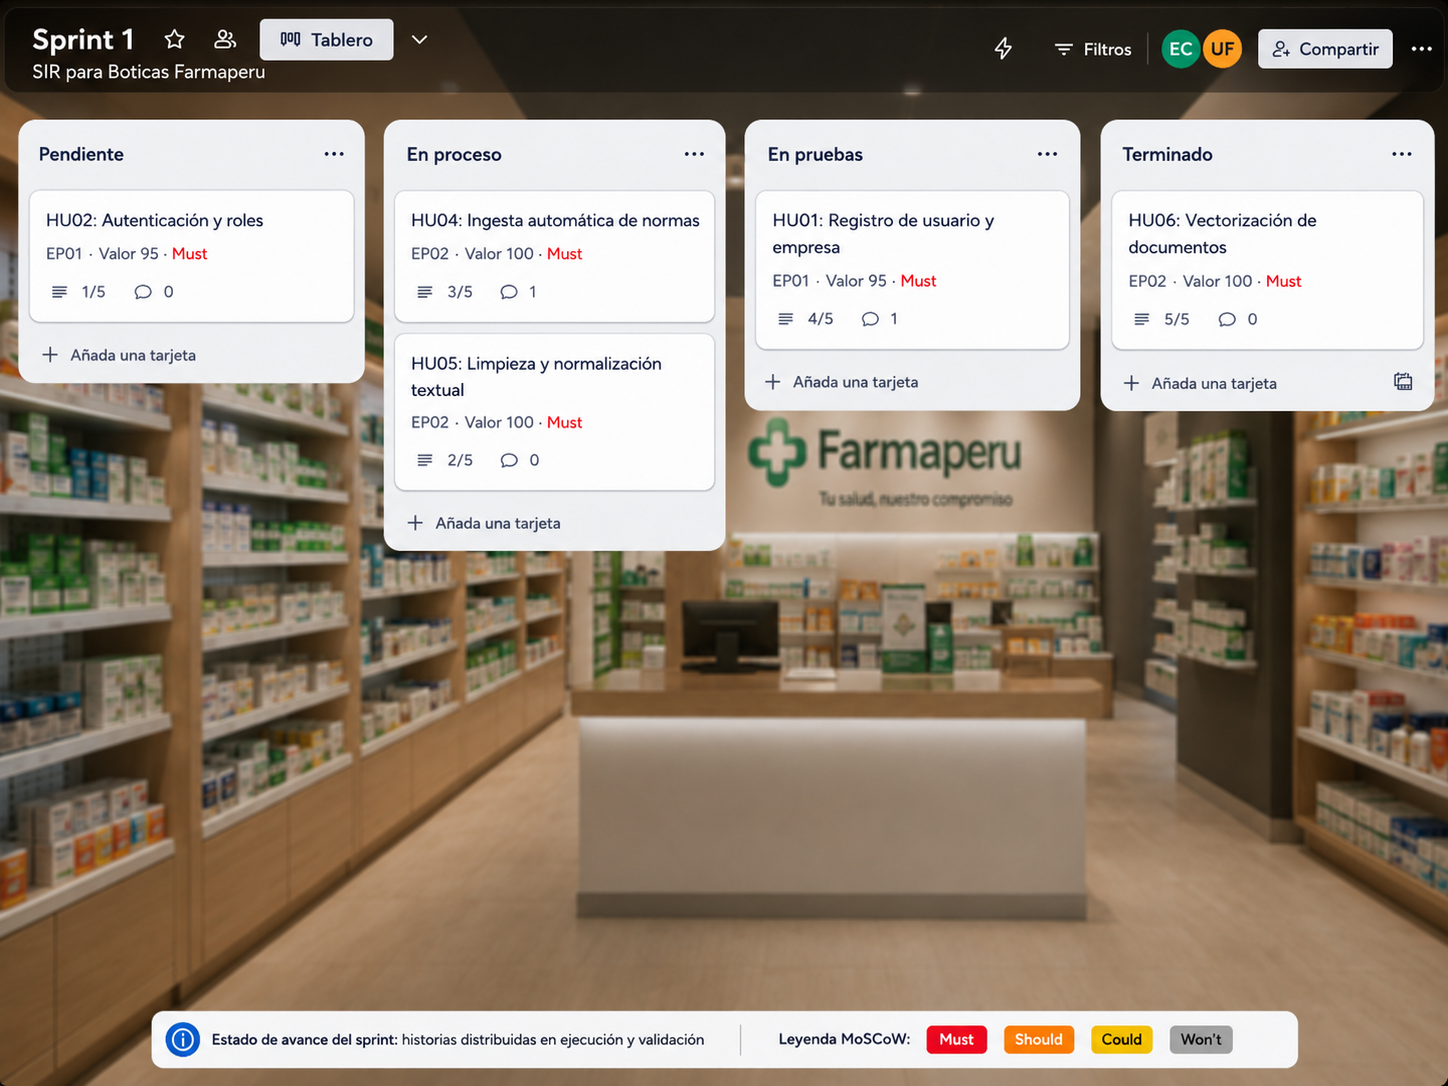
\includegraphics[width=6.5in,height=4.875in]{figuras/docx_image28.png}

\paragraph{4.1.1.8 Resumen del sprint
planning}\label{resumen-del-sprint-planning}

A continuación, se plantea un resumen de lo acordado durante la reunión
de planificación del Sprint:

\begin{itemize}
\item
  Se establecieron los criterios para determinar cuándo una Historia de
  Usuario se considera completada.
\item
  Se seleccionaron las Historias de Usuario HU01, HU02, HU04, HU05 y
  HU06 por su aporte al Producto Mínimo Viable.
\item
  Se utilizó Planning Poker para estimar la dificultad de cada Historia
  de Usuario.
\item
  Se comprometieron 24 story points para el Sprint 1.
\item
  Se definieron tareas técnicas específicas por historia de usuario.
\item
  Se elaboró el Sprint Backlog con prioridades, semanas estimadas y
  responsables.
\item
  Se actualizó el tablero Scrum para visualizar el avance del Sprint.
\item
  Se acordó que la ingesta, limpieza y vectorización deben ser
  verificables sin depender obligatoriamente de OpenAI en este Sprint.
\item
  Se registró que el acta de Sprint Planning debe anexarse como
  evidencia del proyecto.
\end{itemize}

\subsubsection{4.1.2 Construcción del Sprint
1}\label{construcciuxf3n-del-sprint-1}

En esta parte se presentan los componentes construidos durante el Sprint
1, la gestión del Sprint Backlog, la documentación técnica y funcional
relacionada con los elementos implementados, los escenarios de prueba,
las instancias de prueba, los resultados y los acuerdos vinculados al
incremento.

\paragraph{4.1.2.1 Diseño de prototipos}\label{diseuxf1o-de-prototipos}

Para el Sprint 1, se abordaron historias de usuario relacionadas con el
acceso seguro y el pipeline normativo. Los prototipos se orientaron a
validar la navegación principal, el registro de usuario y empresa, el
inicio de sesión, la configuración de fuentes, el monitoreo de ingesta,
la vista de documentos normalizados y la preparación de vectorización.

\phantomsection\label{_Toc231672427}{}Figura 27\\
\emph{HU01 - Resgistro de usuario y empresa}

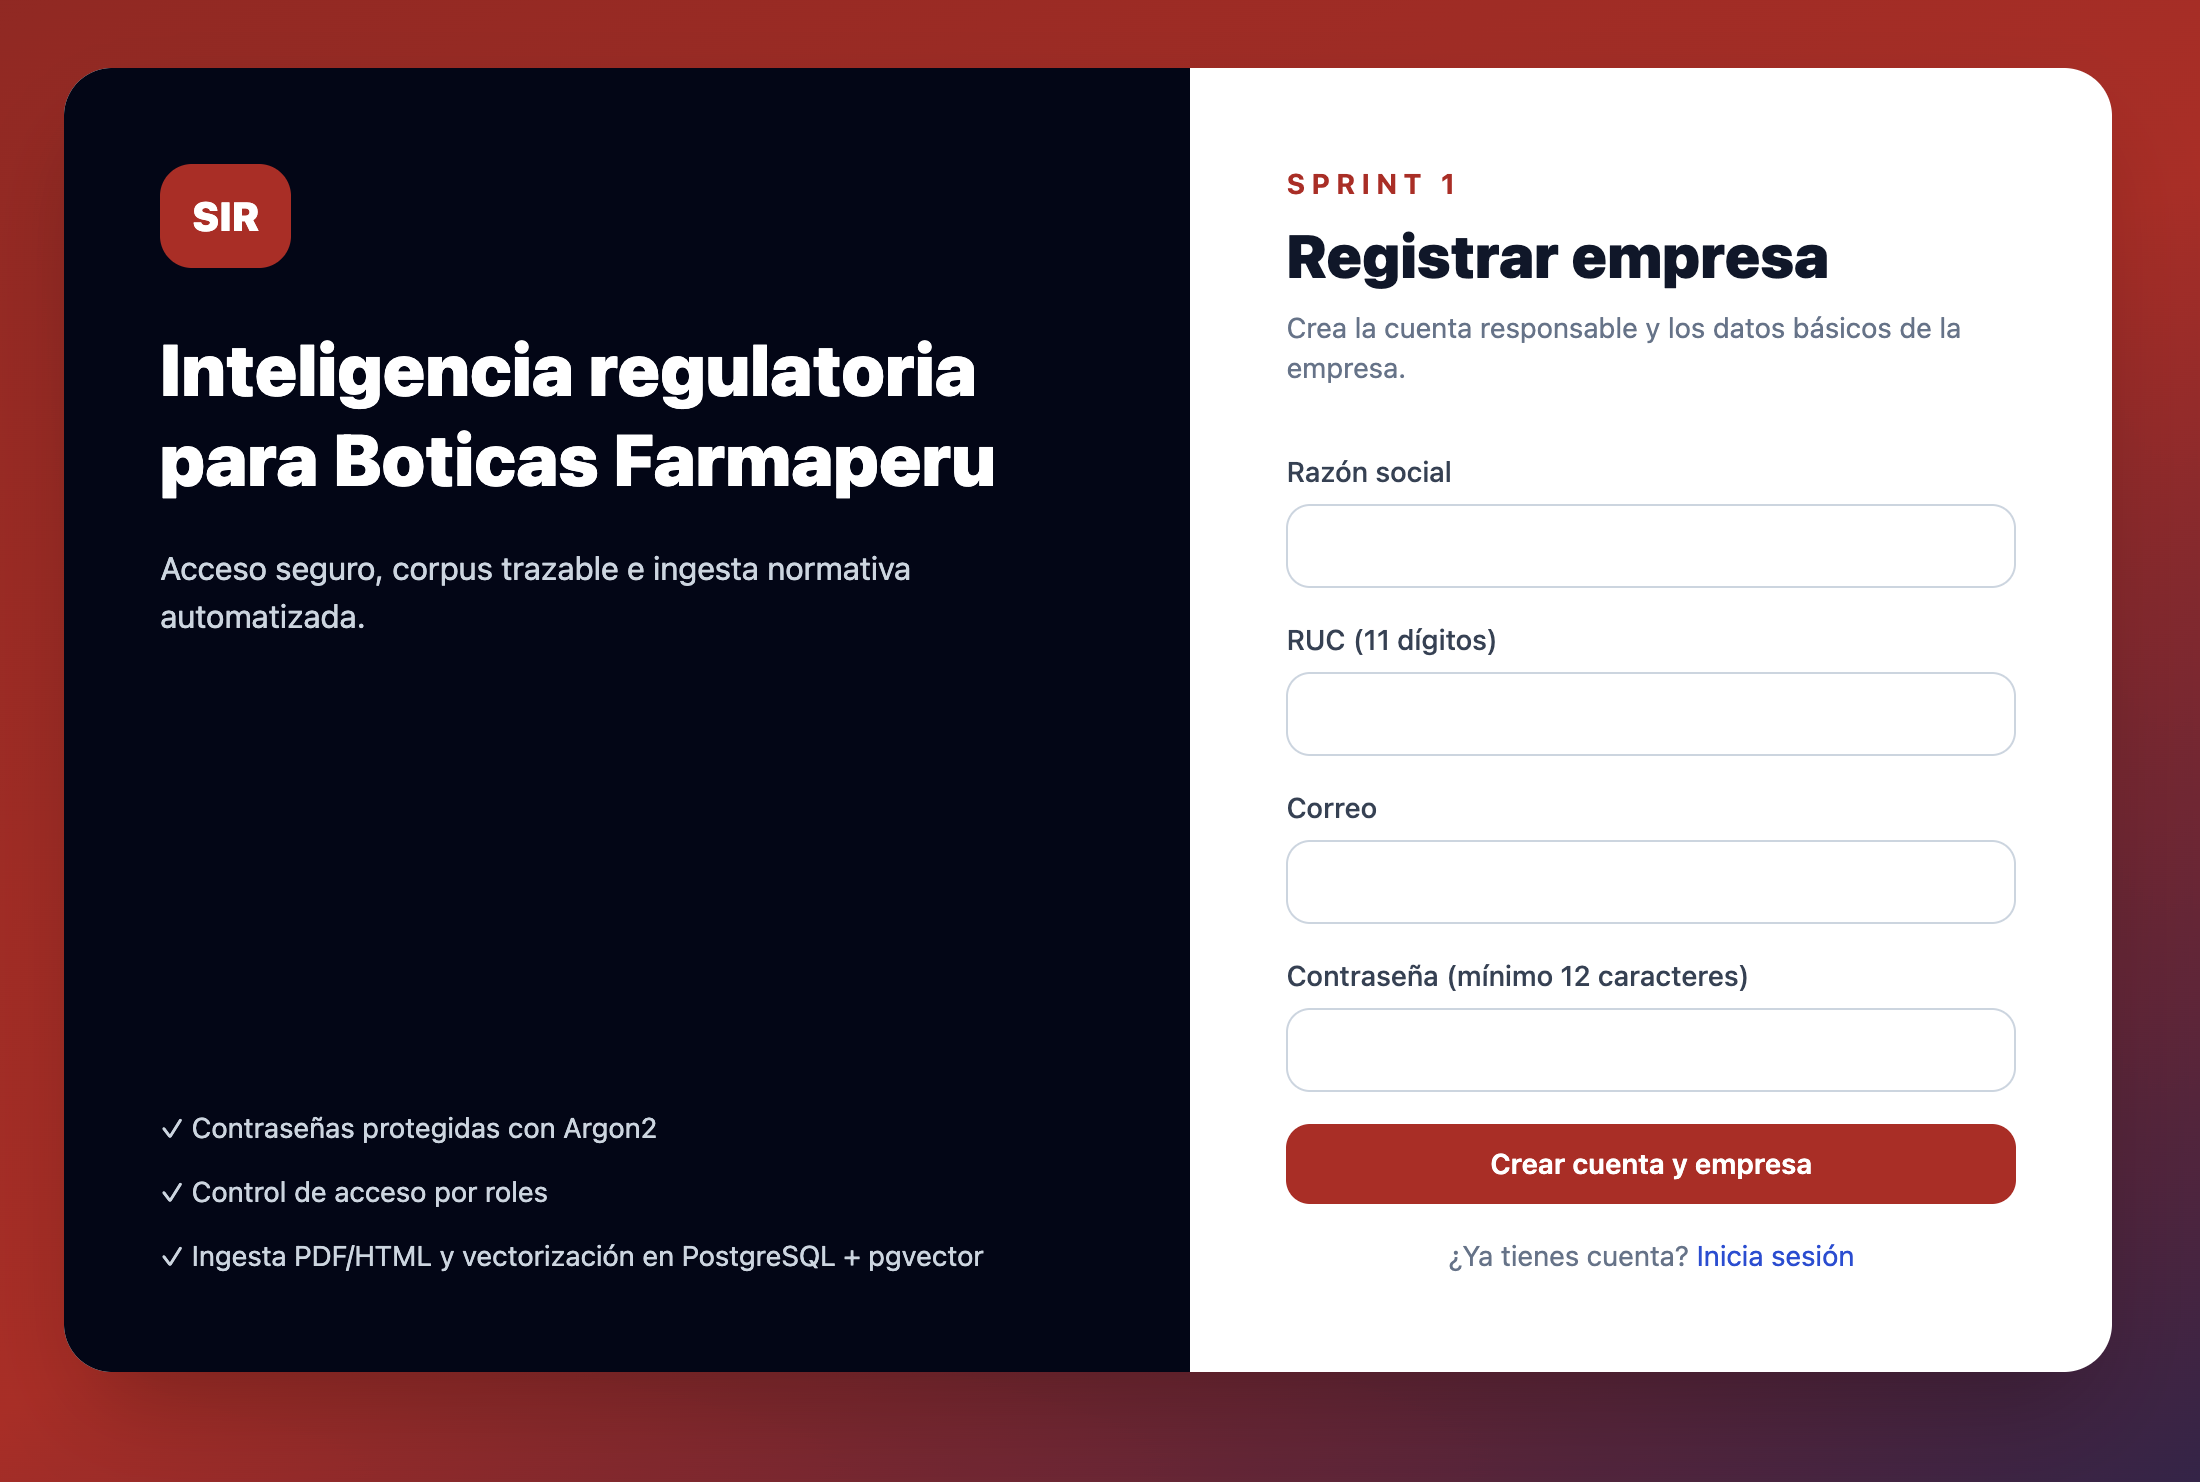
\includegraphics[width=5.37447in,height=3.62031in]{figuras/docx_image29.png}

\phantomsection\label{_Toc231672428}{}Figura 28\\
\emph{HU02 - Autenticación y roles}

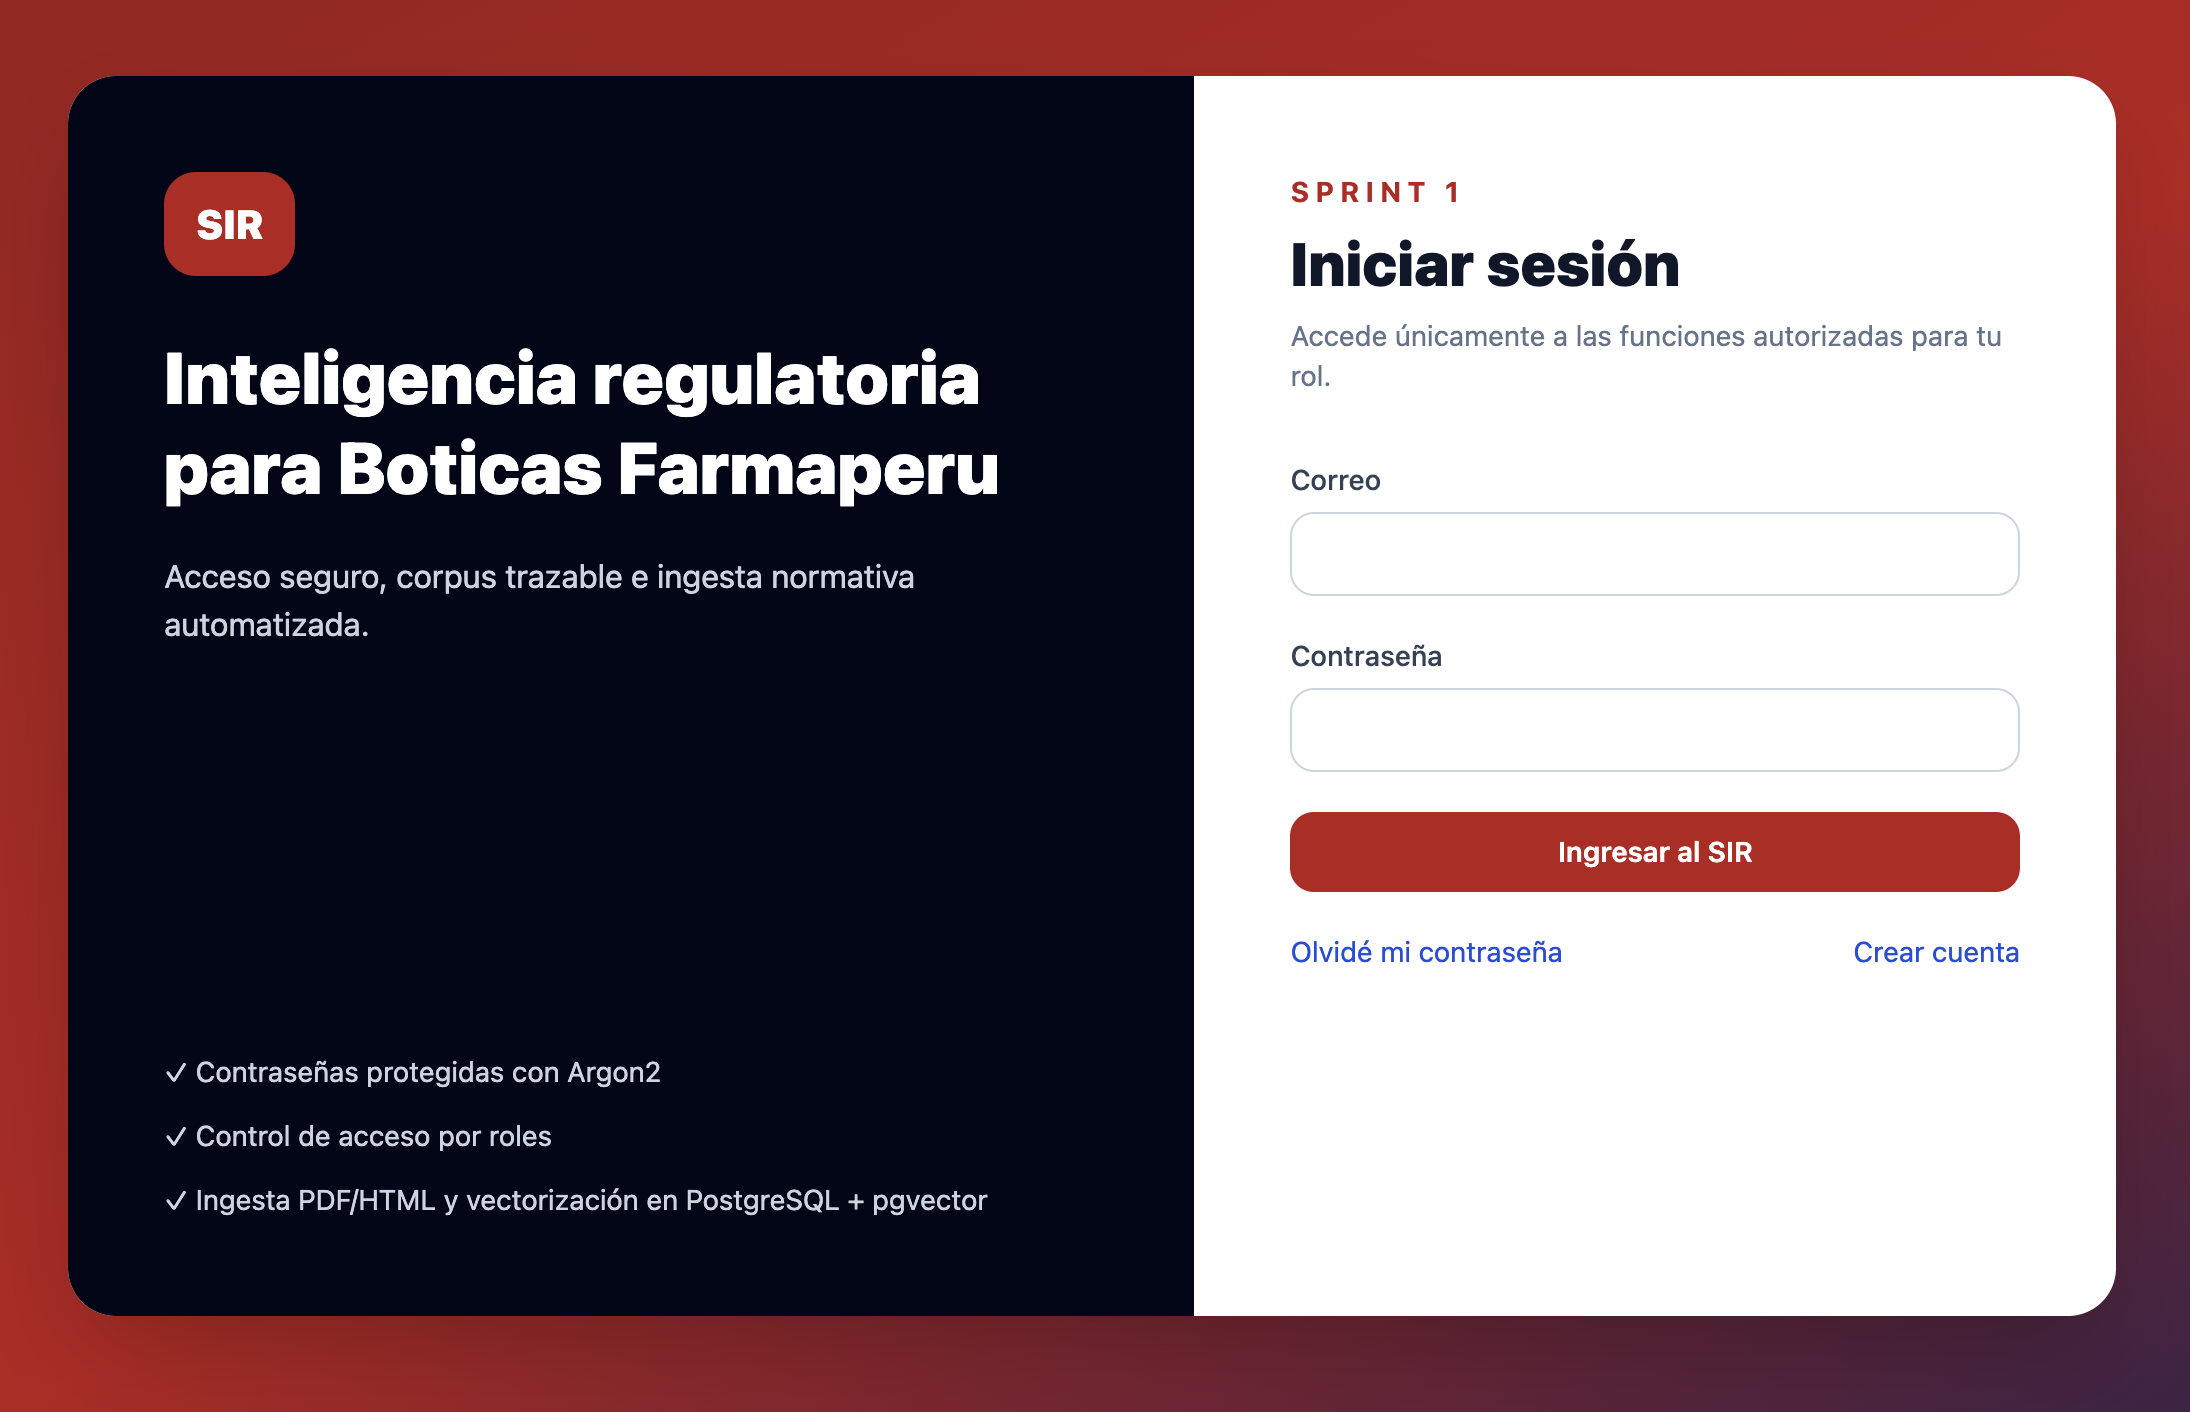
\includegraphics[width=5.36725in,height=3.46061in]{figuras/docx_image30.png}

\phantomsection\label{_Toc231672429}{}Figura 29\\
\emph{HU04 - Ingesta automática de normas}

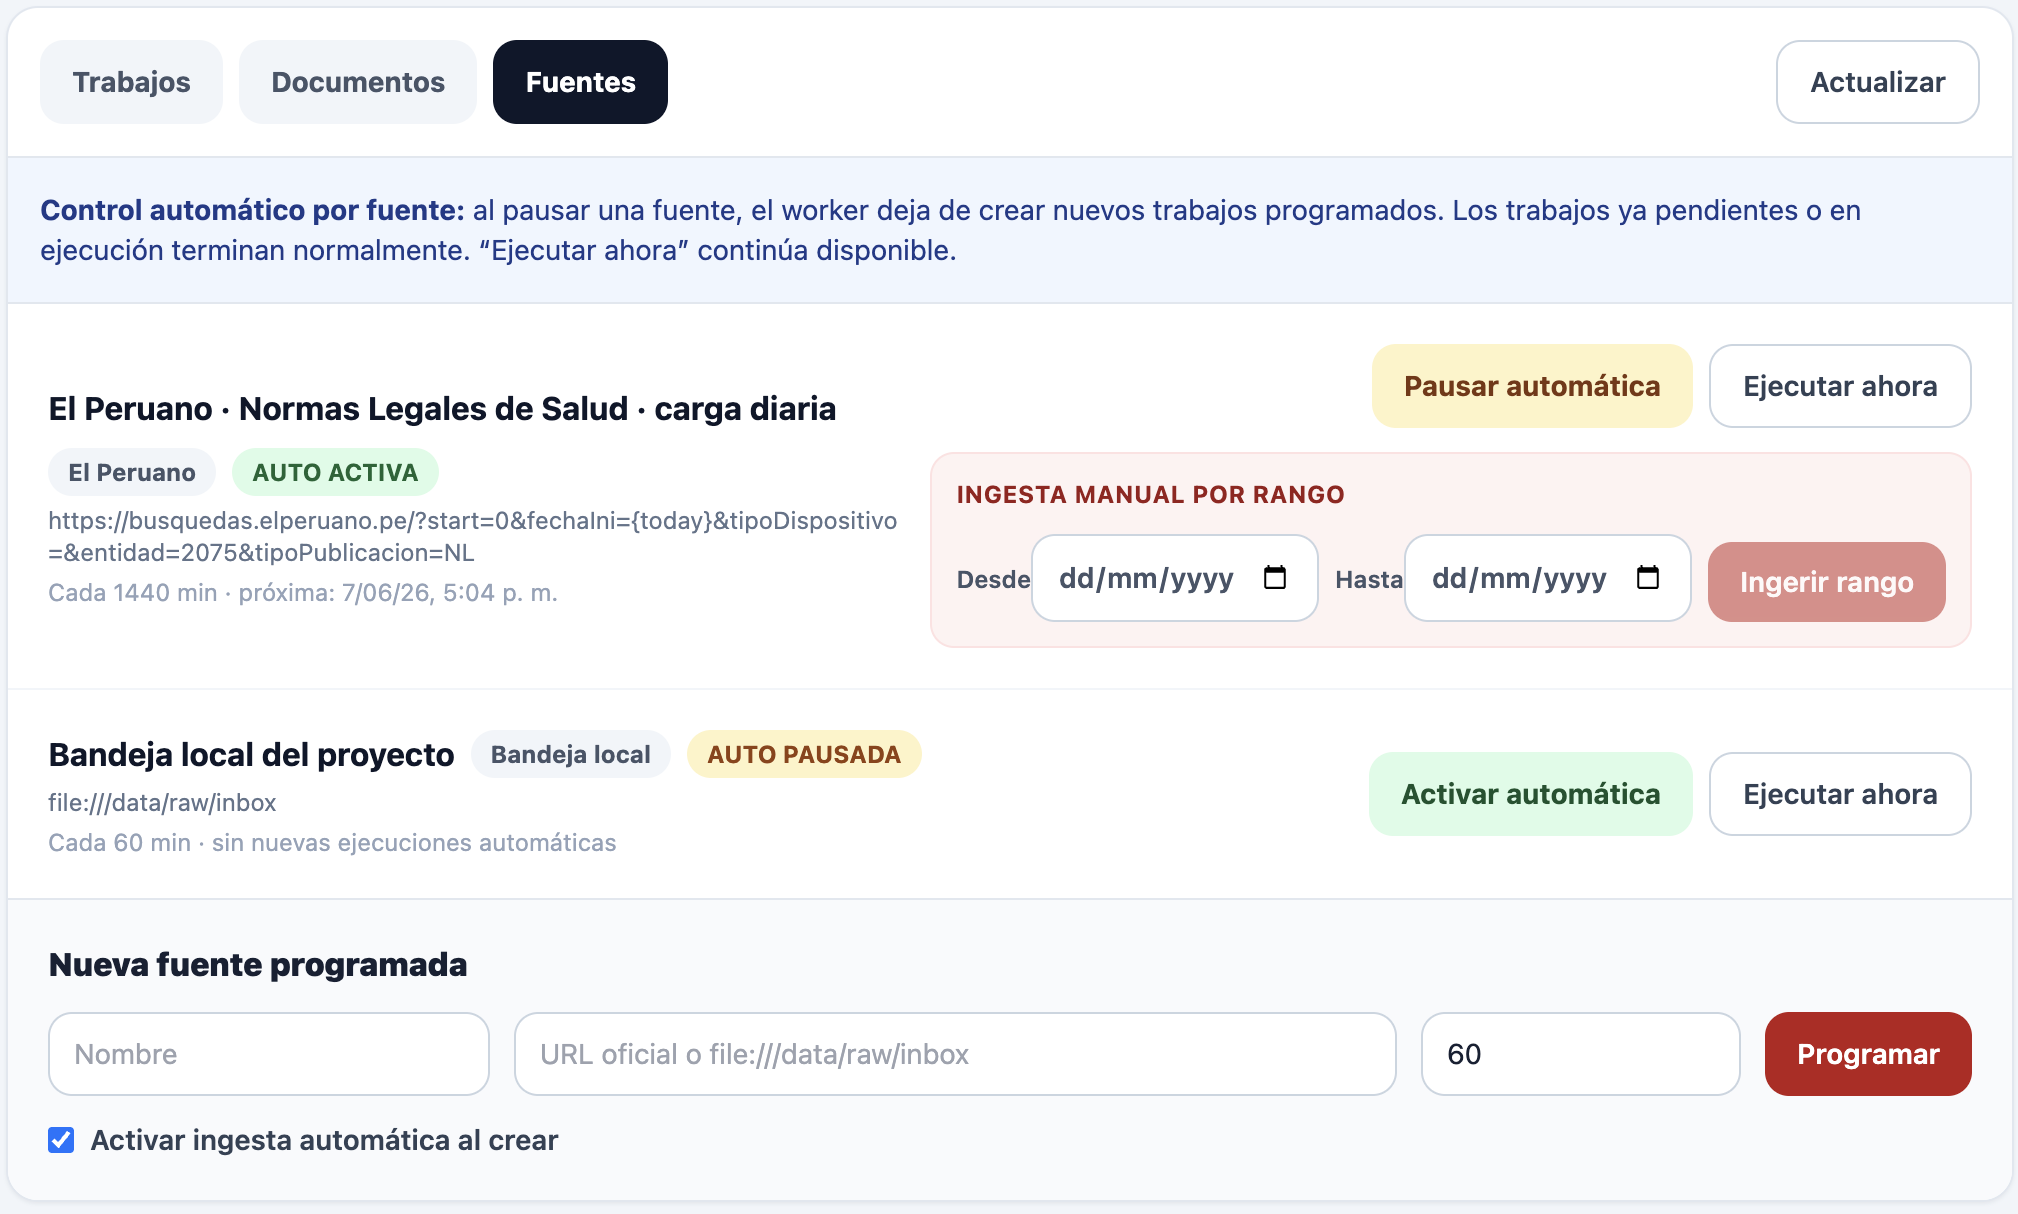
\includegraphics[width=5.58164in,height=3.35793in]{figuras/docx_image31.png}

\phantomsection\label{_Toc231672430}{}Figura 30\\
\emph{HU05 - Limpieza y normalización textual}

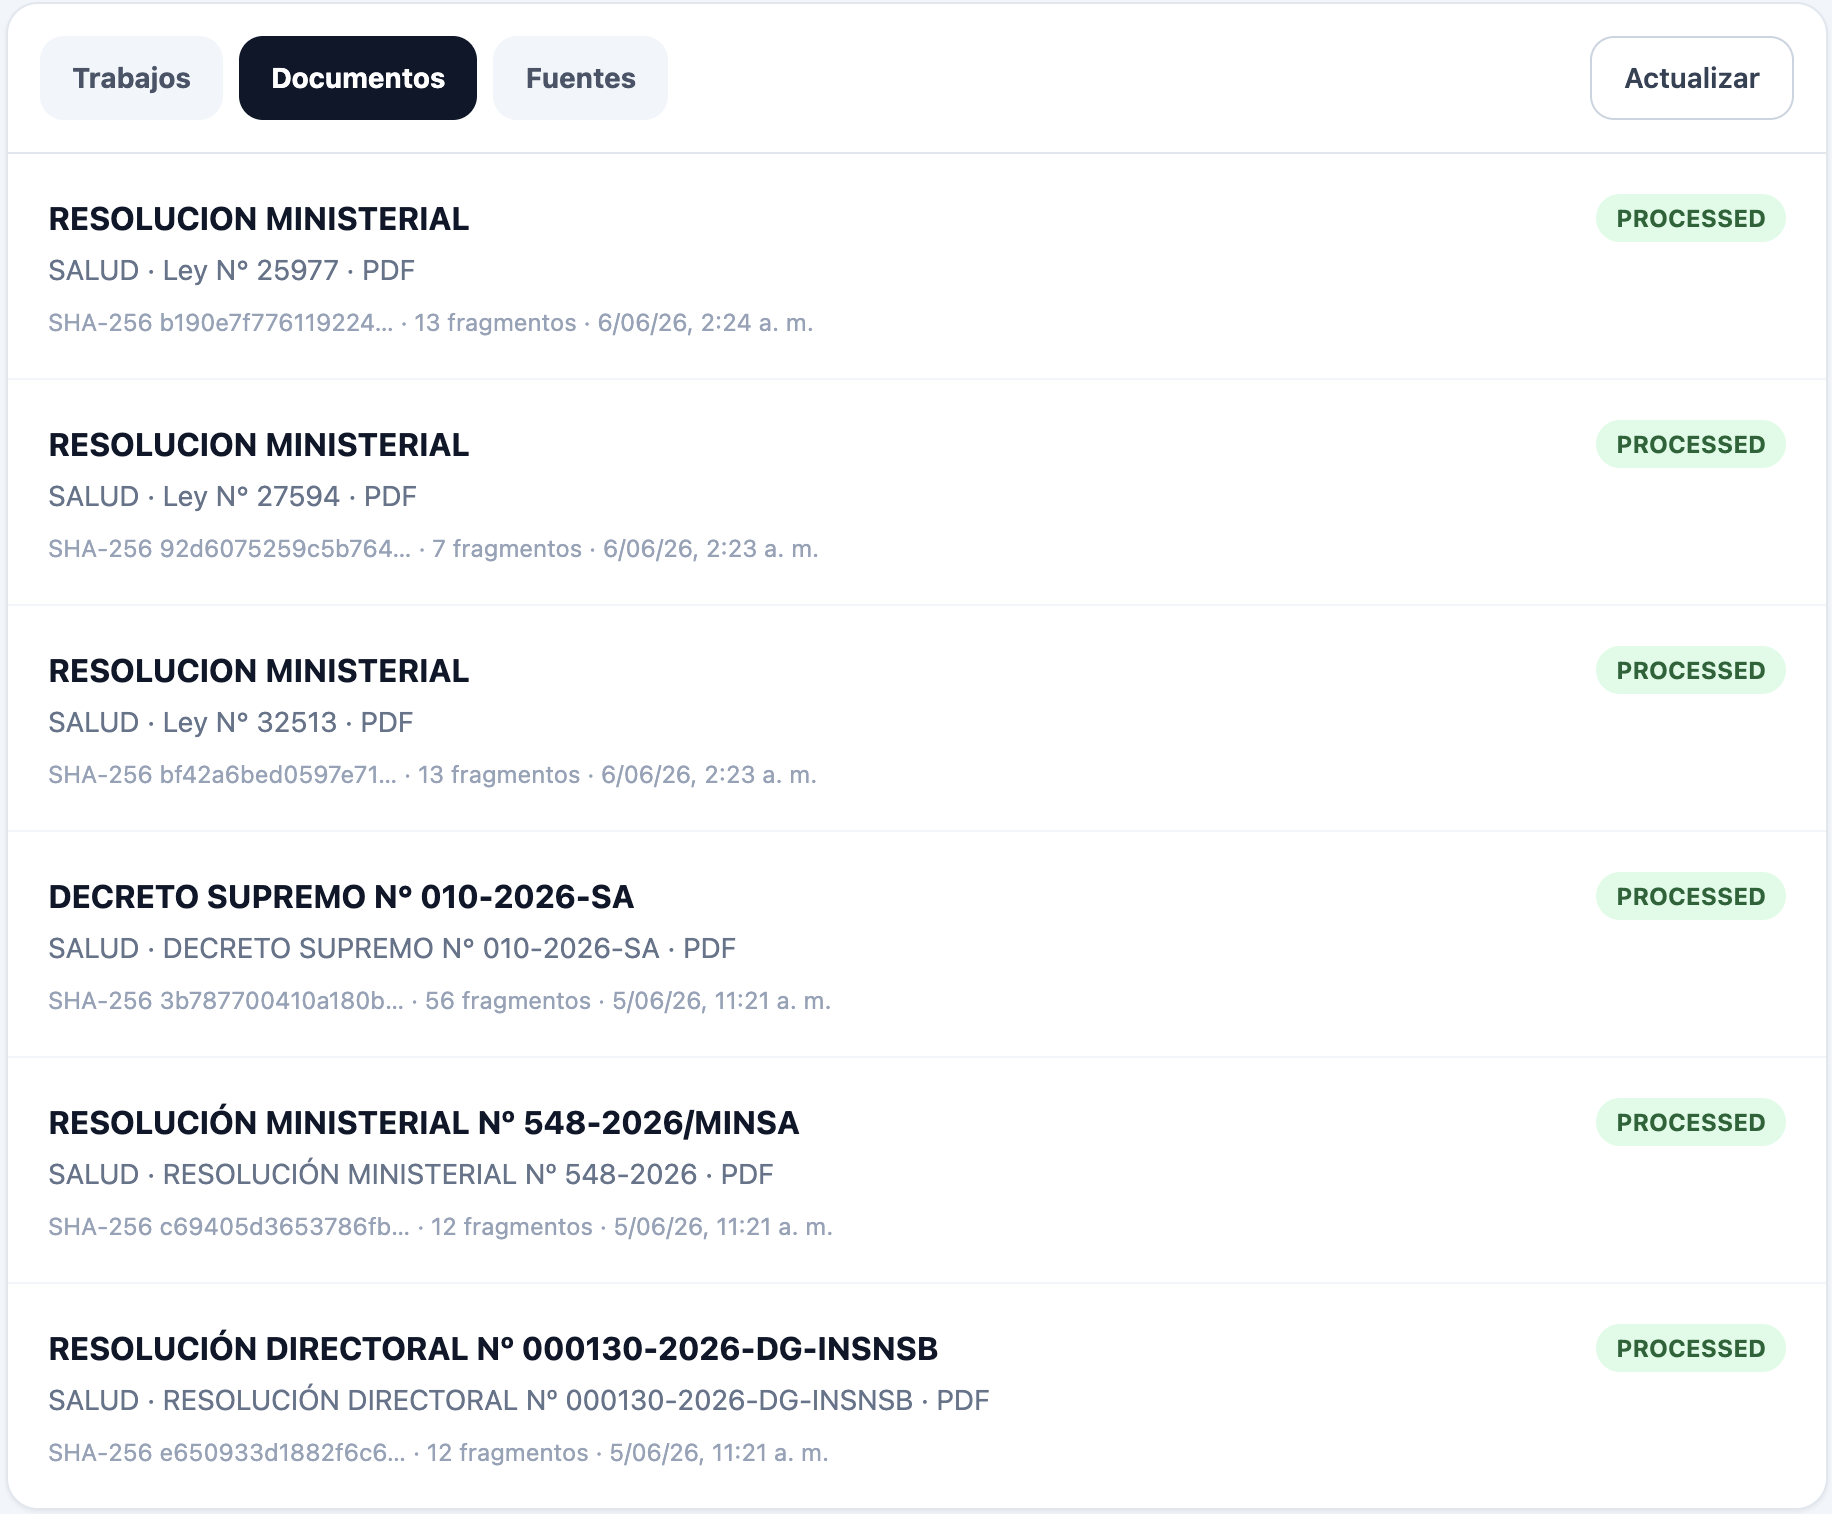
\includegraphics[width=5.58683in,height=3.21474in]{figuras/docx_image32.png}

\phantomsection\label{_Toc231672431}{}Figura 31\\
\emph{HU06 - Vectorización de documentos}

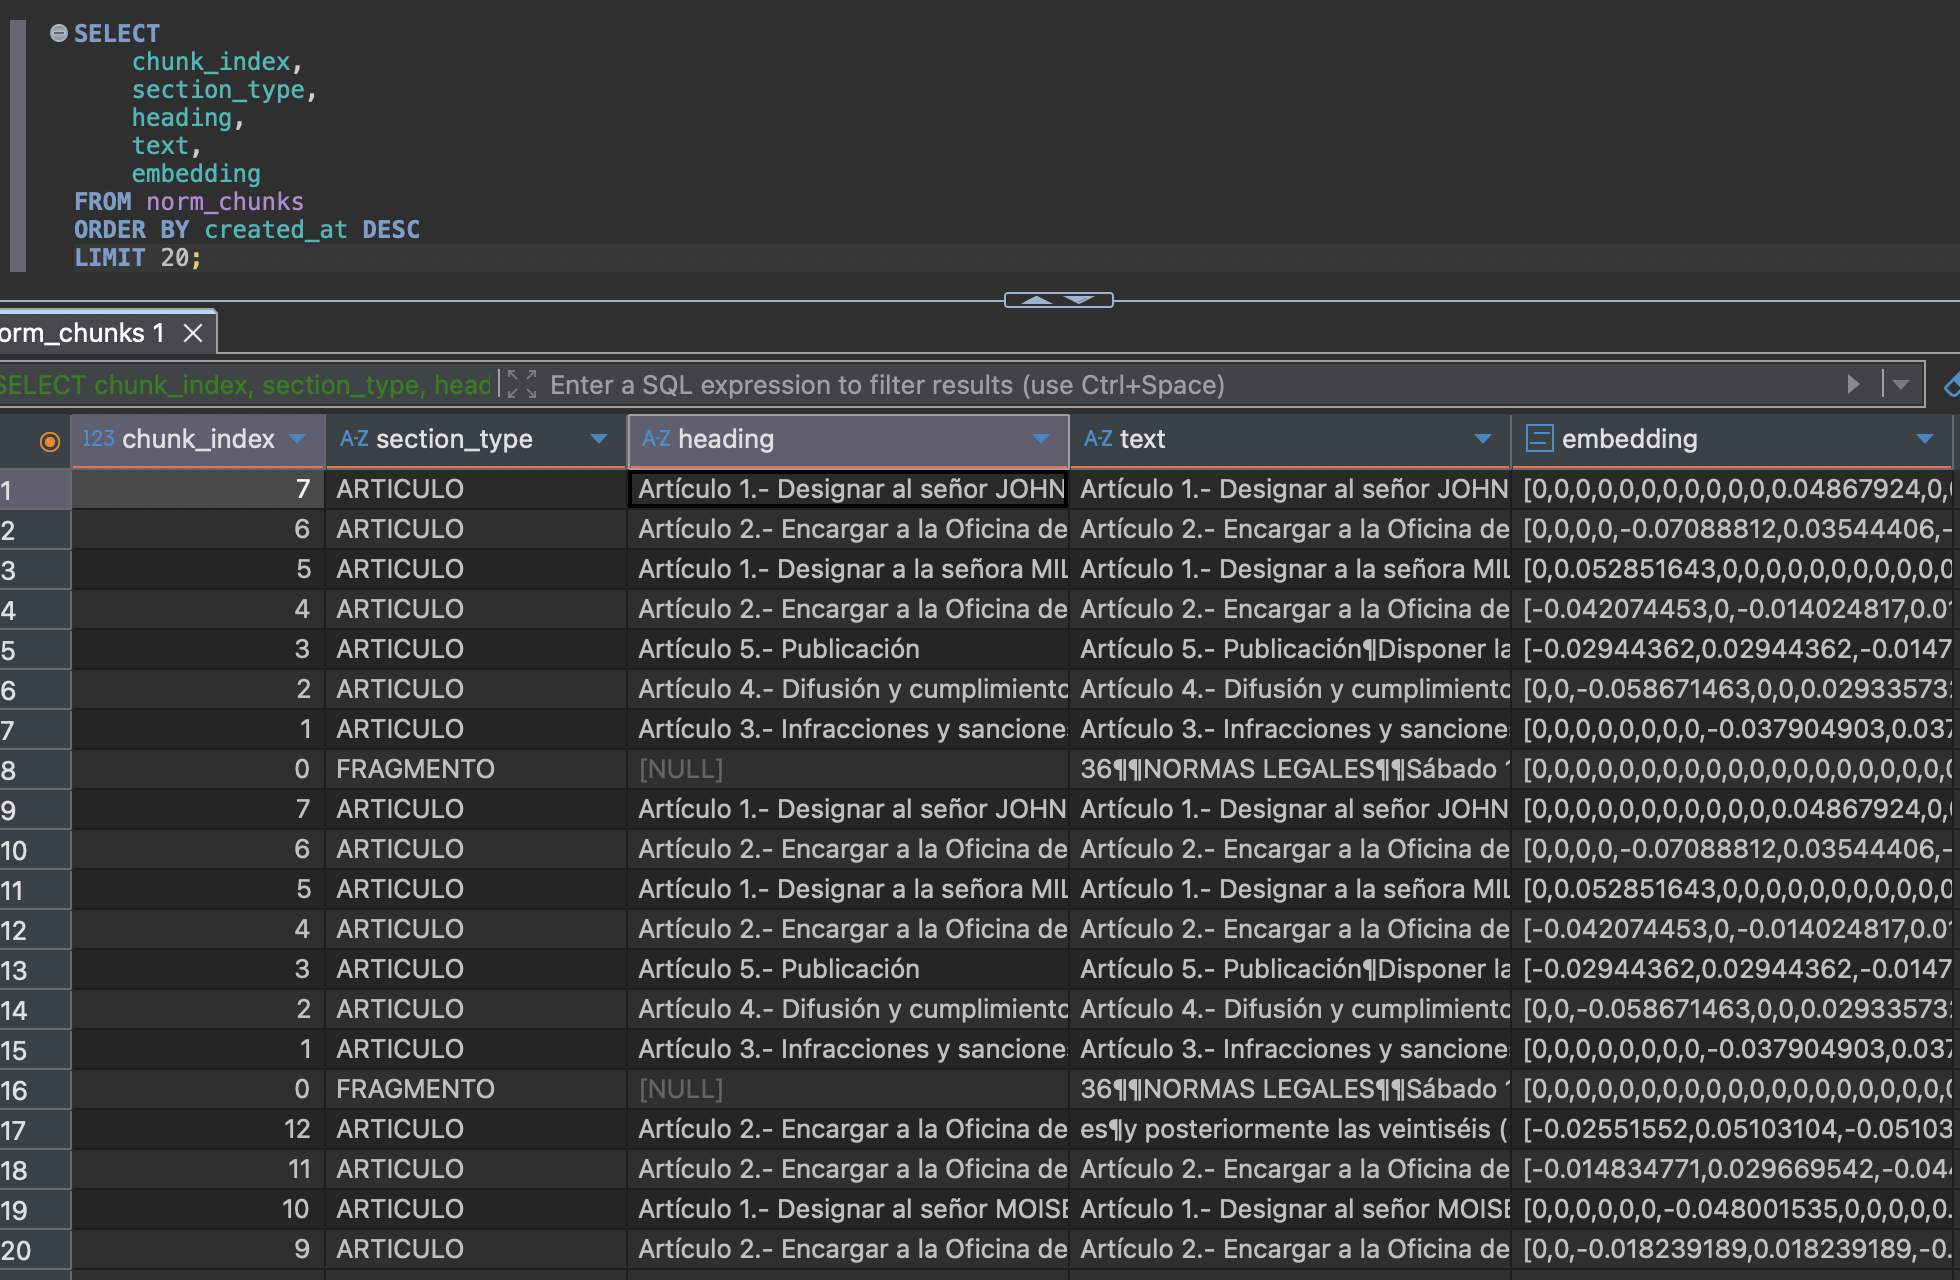
\includegraphics[width=5.91949in,height=3.86601in]{figuras/docx_image33.png}

\paragraph{4.1.2.2 Gestión del Sprint
Backlog}\label{gestiuxf3n-del-sprint-backlog}

Durante la ejecución de este Sprint se logró completar
satisfactoriamente las Historias de Usuario planificadas. Las tareas
fueron ejecutadas de acuerdo con lo establecido en el Sprint Backlog y
en conformidad con los criterios acordados con el Product Owner. La
dependencia más relevante se presentó entre HU04, HU05 y HU06: primero
era necesario obtener documentos normativos, luego normalizarlos y
finalmente preparar sus representaciones semánticas.

\phantomsection\label{_Toc231672432}{}Figura 32\\
\emph{Gestión del tablero Scrum - Sprint 1}

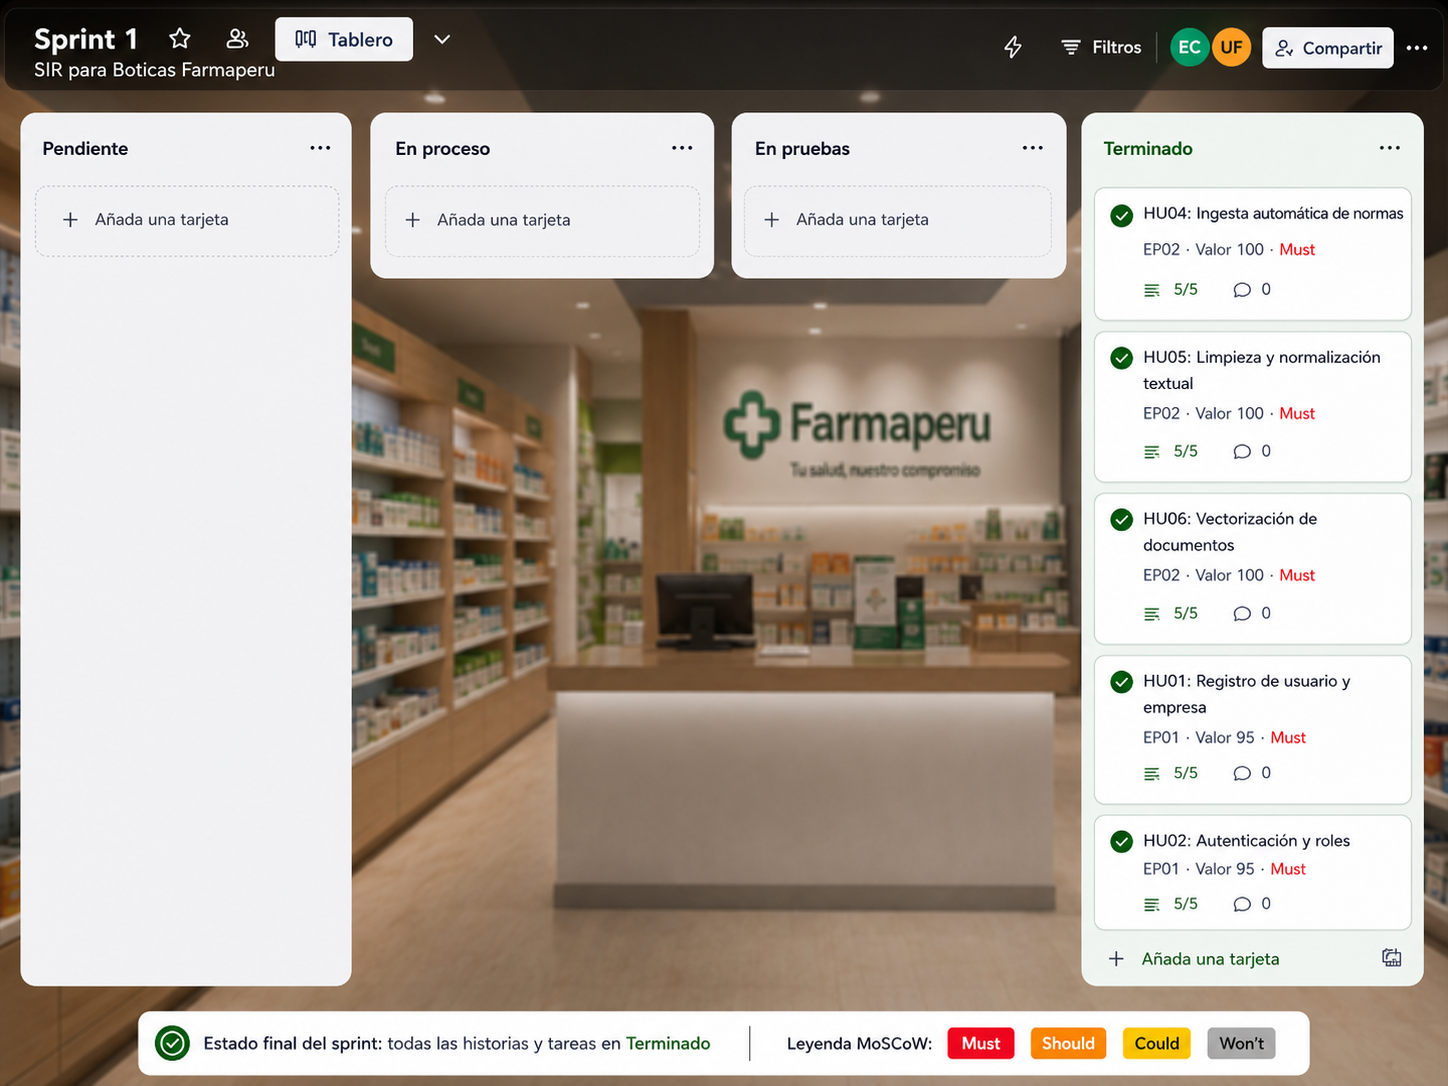
\includegraphics[width=6.5in,height=4.875in]{figuras/docx_image34.png}

\paragraph{4.1.2.3 Documentación funcional y técnica de los componentes
construidos}\label{documentaciuxf3n-funcional-y-tuxe9cnica-de-los-componentes-construidos}

El desarrollo de la documentación técnica y funcional de las HU
consideradas en el Sprint 1 se realizó de la siguiente manera:

\phantomsection\label{_Toc231672286}{}Tabla 31\\
\emph{Descripción funcional y técnica de las HU - Sprint 1}

\begin{longtable}[]{@{}
  >{\raggedright\arraybackslash}p{(\columnwidth - 6\tabcolsep) * \real{0.0597}}
  >{\raggedright\arraybackslash}p{(\columnwidth - 6\tabcolsep) * \real{0.2245}}
  >{\raggedright\arraybackslash}p{(\columnwidth - 6\tabcolsep) * \real{0.3684}}
  >{\raggedright\arraybackslash}p{(\columnwidth - 6\tabcolsep) * \real{0.3474}}@{}}
\toprule\noalign{}
\begin{minipage}[b]{\linewidth}\raggedright
\textbf{HU}
\end{minipage} & \begin{minipage}[b]{\linewidth}\raggedright
\textbf{Descripción}
\end{minipage} & \begin{minipage}[b]{\linewidth}\raggedright
\textbf{Descripción funcional}
\end{minipage} & \begin{minipage}[b]{\linewidth}\raggedright
\textbf{Descripción técnica}
\end{minipage} \\
\midrule\noalign{}
\endhead
\bottomrule\noalign{}
\endlastfoot
HU01 & Registro de usuario y empresa &
\begin{minipage}[t]{\linewidth}\raggedright
1. Mostrar formulario de registro.\\
2. Validar datos obligatorios, correo, RUC y contraseña.\\
3. Solicitar confirmación antes de guardar.\\
4. Crear usuario, empresa y rol inicial.\\
5. Mostrar mensaje de éxito y redirigir al login.\strut
\end{minipage} & Backend con FastAPI y PostgreSQL; modelo User/Company;
hash de contraseña; validaciones de esquema; persistencia
transaccional. \\
HU02 & Autenticacion y roles &
\begin{minipage}[t]{\linewidth}\raggedright
1. Permitir inicio de sesión.\\
2. Denegar acceso con credenciales incorrectas.\\
3. Gestionar sesión/token.\\
4. Restringir rutas por rol.\\
5. Permitir cierre de sesión.\strut
\end{minipage} & Servicio de autenticación; JWT o sesión segura;
middleware de autorización; variables de entorno para secretos; pruebas
de rutas protegidas. \\
HU04 & Ingesta automatica de normas &
\begin{minipage}[t]{\linewidth}\raggedright
1. Ejecutar ingesta por rango de fechas.\\
2. Registrar fuente y documentos descubiertos.\\
3. Descargar o referenciar documentos.\\
4. Guardar metadatos.\\
5. Mostrar logs de ejecución.\strut
\end{minipage} & Job de ingesta; adaptador para El Peruano; tablas
source, document, ingestion\_job e ingestion\_log; checksum; control de
duplicados y estados. \\
HU05 & Limpieza y normalizacion textual &
\begin{minipage}[t]{\linewidth}\raggedright
1. Convertir documentos a texto o Markdown.\\
2. Normalizar contenido.\\
3. Conservar referencias legales.\\
4. Crear fragmentos con metadatos.\\
5. Registrar errores de documentos vacíos.\strut
\end{minipage} & Pipeline de extracción; integración preparada con
MarkItDown; normalizador de texto; segmentador por tamaño/estructura;
tablas document\_text y chunk. \\
HU06 & Vectorizacion de documentos &
\begin{minipage}[t]{\linewidth}\raggedright
1. Seleccionar fragmentos listos.\\
2. Preparar proveedor de embeddings.\\
3. Generar o simular embeddings según configuración.\\
4. Guardar vectores.\\
5. Ejecutar prueba Top-K.\strut
\end{minipage} & Abstracción EmbeddingProvider; pgvector en PostgreSQL;
tabla chunk\_embedding; metadatos de modelo/dimensión; recuperación por
similitud. \\
\end{longtable}

\paragraph{4.1.2.4 Definición de escenarios y casos de
prueba}\label{definiciuxf3n-de-escenarios-y-casos-de-prueba}

A continuación, se exponen los escenarios y casos de prueba diseñados
para validar el cumplimiento de los criterios de aceptación definidos en
cada Historia de Usuario.

\phantomsection\label{_Toc231672287}{}Tabla 32\\
\emph{Escenarios y casos de prueba - Sprint 1}

\begin{longtable}[]{@{}
  >{\raggedright\arraybackslash}p{(\columnwidth - 14\tabcolsep) * \real{0.0657}}
  >{\raggedright\arraybackslash}p{(\columnwidth - 14\tabcolsep) * \real{0.0765}}
  >{\raggedright\arraybackslash}p{(\columnwidth - 14\tabcolsep) * \real{0.1203}}
  >{\raggedright\arraybackslash}p{(\columnwidth - 14\tabcolsep) * \real{0.2625}}
  >{\raggedright\arraybackslash}p{(\columnwidth - 14\tabcolsep) * \real{0.1641}}
  >{\raggedright\arraybackslash}p{(\columnwidth - 14\tabcolsep) * \real{0.1312}}
  >{\raggedright\arraybackslash}p{(\columnwidth - 14\tabcolsep) * \real{0.0984}}
  >{\raggedright\arraybackslash}p{(\columnwidth - 14\tabcolsep) * \real{0.0812}}@{}}
\toprule\noalign{}
\multirow{2}{=}{\begin{minipage}[b]{\linewidth}\raggedright
\textbf{HU}
\end{minipage}} &
\multirow{2}{=}{\begin{minipage}[b]{\linewidth}\raggedright
\textbf{Caso de prueba}
\end{minipage}} &
\multicolumn{3}{>{\raggedright\arraybackslash}p{(\columnwidth - 14\tabcolsep) * \real{0.5469} + 4\tabcolsep}}{%
\begin{minipage}[b]{\linewidth}\raggedright
\textbf{Casos de prueba}
\end{minipage}} &
\multirow{2}{=}{\begin{minipage}[b]{\linewidth}\raggedright
\textbf{Datos de prueba}
\end{minipage}} &
\multirow{2}{=}{\begin{minipage}[b]{\linewidth}\raggedright
\textbf{Tipo}
\end{minipage}} &
\multirow{2}{=}{\begin{minipage}[b]{\linewidth}\raggedright
\textbf{Responsable}
\end{minipage}} \\
& & \begin{minipage}[b]{\linewidth}\raggedright
\textbf{Descripción}
\end{minipage} & \begin{minipage}[b]{\linewidth}\raggedright
\textbf{Secuencia}
\end{minipage} & \begin{minipage}[b]{\linewidth}\raggedright
\textbf{Resultado}
\end{minipage} \\
\midrule\noalign{}
\endhead
\bottomrule\noalign{}
\endlastfoot
HU01 & CP001 & Registro de usuario y empresa &
\begin{minipage}[t]{\linewidth}\raggedright
1. Ingresar datos válidos.\\
2. Confirmar registro.\\
3. Verificar usuario y empresa creados.\\
4. Probar correo/RUC duplicado.\strut
\end{minipage} & Registro exitoso, validaciones correctas y contraseña
protegida. & Responsable administrativo & Funcional & Jadir H. / Khail
M. \\
HU02 & CP002 & Autenticacion y roles &
\begin{minipage}[t]{\linewidth}\raggedright
1. Iniciar sesión con credenciales válidas.\\
2. Intentar acceder sin token.\\
3. Iniciar con credenciales inválidas.\\
4. Cerrar sesión.\strut
\end{minipage} & Acceso permitido solo con credenciales válidas y rol
autorizado. & Usuario registrado & Funcional / Seguridad & Jadir H. /
Khail M. \\
HU04 & CP003 & Ingesta automatica de normas &
\begin{minipage}[t]{\linewidth}\raggedright
1. Ejecutar ingesta por rango.\\
2. Validar metadatos.\\
3. Verificar duplicados.\\
4. Probar rango sin resultados.\strut
\end{minipage} & Documentos y logs registrados; duplicados omitidos;
rango vacío informado sin falla crítica. & Sistema & Integración & Jadir
H. / Khail M. \\
HU05 & CP004 & Limpieza y normalizacion textual &
\begin{minipage}[t]{\linewidth}\raggedright
1. Procesar documento descargado.\\
2. Revisar texto limpio.\\
3. Verificar fragmentos.\\
4. Probar documento ilegible.\strut
\end{minipage} & Texto normalizado y fragmentos con metadatos; error
controlado para documentos inválidos. & Sistema & Técnica & Jadir H. /
Khail M. \\
HU06 & CP005 & Vectorizacion de documentos &
\begin{minipage}[t]{\linewidth}\raggedright
1. Seleccionar fragmentos listos.\\
2. Ejecutar vectorización o dry-run.\\
3. Consultar pgvector.\\
4. Validar Top-K.\strut
\end{minipage} & Vector asociado a chunk y documento; recuperación
semántica básica operativa. & Sistema & Técnica / Integración & Jadir H.
/ Khail M. \\
\end{longtable}

\paragraph{4.1.2.5 Resultados de pruebas internas de los
desarrolladores}\label{resultados-de-pruebas-internas-de-los-desarrolladores}

Los resultados obtenidos tras ejecutar las pruebas correspondientes
permitieron verificar el logro de los criterios definidos en el DoD. En
este sprint se priorizaron pruebas funcionales y técnicas, porque el
incremento habilita la arquitectura RAG pero aún no valida la generación
final de respuestas con IA. Como evidencia se consideran los registros
de ejecución, logs del pipeline, resultados de pruebas unitarias y
conformidad del incremento por parte del Product Owner.

\begin{itemize}
\item
  Se verificó que el registro de usuario y empresa almacene datos
  obligatorios y rechace duplicados.
\item
  Se verificó que la autenticación proteja rutas y no exponga
  credenciales.
\item
  Se verificó que la ingesta genere logs aun cuando no existan
  documentos para un rango de fechas.
\item
  Se verificó que la limpieza textual conserve metadatos necesarios para
  citación posterior.
\item
  Se verificó que la vectorización quede preparada con pgvector y
  proveedor configurable.
\item
  Se registró como acción técnica la revisión de empaquetado del backend
  para evitar errores de importación en pruebas Docker/pytest.
\end{itemize}

\paragraph{4.1.2.6 Resultados de las pruebas realizadas en el sprint
1}\label{resultados-de-las-pruebas-realizadas-en-el-sprint-1}

A continuación, se exponen los hallazgos derivados de la ejecución de
las pruebas correspondientes, los cuales validan el comportamiento del
sistema frente a los escenarios diseñados.

\phantomsection\label{_Toc231672288}{}Tabla 33\\
\emph{Listado de pruebas - Sprint 1}

\begin{longtable}[]{@{}
  >{\raggedright\arraybackslash}p{(\columnwidth - 12\tabcolsep) * \real{0.0664}}
  >{\raggedright\arraybackslash}p{(\columnwidth - 12\tabcolsep) * \real{0.1647}}
  >{\raggedright\arraybackslash}p{(\columnwidth - 12\tabcolsep) * \real{0.2526}}
  >{\raggedright\arraybackslash}p{(\columnwidth - 12\tabcolsep) * \real{0.1648}}
  >{\raggedright\arraybackslash}p{(\columnwidth - 12\tabcolsep) * \real{0.1098}}
  >{\raggedright\arraybackslash}p{(\columnwidth - 12\tabcolsep) * \real{0.1099}}
  >{\raggedright\arraybackslash}p{(\columnwidth - 12\tabcolsep) * \real{0.1318}}@{}}
\toprule\noalign{}
\begin{minipage}[b]{\linewidth}\raggedright
\textbf{HU}
\end{minipage} & \begin{minipage}[b]{\linewidth}\raggedright
\textbf{Descripción}
\end{minipage} & \begin{minipage}[b]{\linewidth}\raggedright
\textbf{Ejecución}
\end{minipage} & \begin{minipage}[b]{\linewidth}\raggedright
\textbf{Resultado}
\end{minipage} & \begin{minipage}[b]{\linewidth}\raggedright
\textbf{Estado}
\end{minipage} & \begin{minipage}[b]{\linewidth}\raggedright
\textbf{Fecha}
\end{minipage} & \begin{minipage}[b]{\linewidth}\raggedright
\textbf{Autor}
\end{minipage} \\
\midrule\noalign{}
\endhead
\bottomrule\noalign{}
\endlastfoot
HU01 & Se registra usuario y empresa & Ejecutar registro con datos
válidos y confirmar operación. & Usuario y empresa asociados
correctamente. & Aprobado & Semana 2 & Jadir H. \\
HU01 & Validación de RUC/correo duplicado & Registrar datos repetidos. &
El sistema bloquea duplicidad y muestra mensaje. & Aprobado & Semana 2 &
Khail M. \\
HU02 & Inicio y cierre de sesión & Login válido, acceso a ruta protegida
y logout. & Sesión creada y cerrada correctamente. & Aprobado & Semana 3
& Jadir H. \\
HU02 & Acceso denegado sin rol & Intentar ruta protegida sin sesión o
rol. & Acceso denegado. & Aprobado & Semana 3 & Khail M. \\
HU04 & Ingesta por rango de fechas & Ejecutar job sobre fuente
configurada. & Log creado con resultados y estado. & Aprobado & Semana 6
& Jadir H. \\
\end{longtable}

\paragraph{4.1.2.7 Cumplimiento de DoD del sprint
1}\label{cumplimiento-de-dod-del-sprint-1}

\phantomsection\label{_Toc231672289}{}Tabla 34\\
\emph{Lista de conformidad según criterios DoD - Sprint 1}

\begin{longtable}[]{@{}
  >{\raggedright\arraybackslash}p{(\columnwidth - 6\tabcolsep) * \real{0.0757}}
  >{\raggedright\arraybackslash}p{(\columnwidth - 6\tabcolsep) * \real{0.3532}}
  >{\raggedright\arraybackslash}p{(\columnwidth - 6\tabcolsep) * \real{0.4021}}
  >{\raggedright\arraybackslash}p{(\columnwidth - 6\tabcolsep) * \real{0.1689}}@{}}
\toprule\noalign{}
\begin{minipage}[b]{\linewidth}\raggedright
\textbf{ID}
\end{minipage} & \begin{minipage}[b]{\linewidth}\raggedright
\textbf{Criterio DoD}
\end{minipage} & \begin{minipage}[b]{\linewidth}\raggedright
\textbf{Evidencia}
\end{minipage} & \begin{minipage}[b]{\linewidth}\raggedright
\textbf{¿Concluído?}
\end{minipage} \\
\midrule\noalign{}
\endhead
\bottomrule\noalign{}
\endlastfoot
1 & Funcionalidad responde a la necesidad del Sprint & HU01, HU02, HU04,
HU05 y HU06 implementadas o preparadas según alcance. & Ok \\
2 & Criterios de aceptación verificados & Casos de prueba CP001 a CP005
ejecutados. & Ok \\
3 & Ausencia de defectos críticos & No se registran defectos bloqueantes
al cierre del Sprint. & Ok \\
4 & Documentación técnica y funcional actualizada & Tablas de
descripción funcional/técnica y pruebas incluidas en el capítulo. &
Ok \\
5 & Seguridad de credenciales & Uso de hash y variables de entorno para
secretos. & Ok \\
6 & Trazabilidad documental & Metadatos de fuente, documento, texto,
chunk y vector preparados. & Ok \\
7 & Aprobación del Product Owner & Conformidad del incremento base para
continuar con Sprint 2. & Ok \\
\end{longtable}

\paragraph{4.1.2.8 Gestión de acuerdos del
sprint}\label{gestiuxf3n-de-acuerdos-del-sprint}

Durante el primer Sprint se formalizaron acuerdos orientados a asegurar
coherencia técnica y académica del proyecto:

\begin{itemize}
\item
  El Sprint 1 se limita al acceso seguro y preparación del corpus
  normativo; la generación conversacional se valida en Sprint 2.
\item
  La base vectorial del proyecto será pgvector para mantener una
  arquitectura inicial más simple y económica con PostgreSQL.
\item
  La ingesta de El Peruano debe registrar logs incluso cuando el
  resultado sea cero documentos encontrados.
\item
  MarkItDown se considera alternativa para conversión a Markdown; si se
  requiere extracción de imágenes, se evaluará una herramienta
  complementaria.
\item
  OpenAI se mantiene como proveedor configurable, pero no como requisito
  indispensable para aprobar Sprint 1.
\item
  Toda respuesta futura del asistente deberá mostrar fuente oficial y
  advertir que no constituye asesoría legal vinculante.
\end{itemize}

\subsubsection{4.1.3 Daily Meeting}\label{daily-meeting}

Durante el desarrollo del Sprint 1, se realizaron reuniones de
seguimiento con el propósito de sincronizar avances, identificar
impedimentos y actualizar el tablero Scrum. En cada reunión se revisaron
las tres preguntas base: qué se avanzó, qué se realizará y qué
obstáculos existen.

\paragraph{4.1.3.1 Frecuencia de
reuniones}\label{frecuencia-de-reuniones}

La frecuencia de reuniones fue de dos sesiones por semana,
principalmente los lunes y jueves. Esta cadencia fue suficiente para un
equipo pequeño y permitió atender oportunamente bloqueos relacionados
con configuración de entorno, ingesta normativa y preparación de datos.

\paragraph{4.1.3.2 Gestión del tablero en el
sprint}\label{gestiuxf3n-del-tablero-en-el-sprint}

La frecuencia de reuniones fue de dos sesiones por semana,
principalmente los lunes y jueves. Esta cadencia fue suficiente para un
equipo pequeño y permitió atender oportunamente bloqueos relacionados
con configuración de entorno, ingesta normativa y preparación de datos.

\phantomsection\label{_Toc231672290}{}Tabla 35\\
\emph{Consolidación de Daily Meetings - Sprint 1}

\begin{longtable}[]{@{}
  >{\raggedright\arraybackslash}p{(\columnwidth - 10\tabcolsep) * \real{0.0983}}
  >{\raggedright\arraybackslash}p{(\columnwidth - 10\tabcolsep) * \real{0.1304}}
  >{\raggedright\arraybackslash}p{(\columnwidth - 10\tabcolsep) * \real{0.2499}}
  >{\raggedright\arraybackslash}p{(\columnwidth - 10\tabcolsep) * \real{0.1630}}
  >{\raggedright\arraybackslash}p{(\columnwidth - 10\tabcolsep) * \real{0.1304}}
  >{\raggedright\arraybackslash}p{(\columnwidth - 10\tabcolsep) * \real{0.2281}}@{}}
\toprule\noalign{}
\begin{minipage}[b]{\linewidth}\raggedright
\textbf{Día}
\end{minipage} & \begin{minipage}[b]{\linewidth}\raggedright
\textbf{Participantes}
\end{minipage} & \begin{minipage}[b]{\linewidth}\raggedright
\textbf{¿Qué hiciste ayer?}
\end{minipage} & \begin{minipage}[b]{\linewidth}\raggedright
\textbf{¿Qué harás hoy?}
\end{minipage} & \begin{minipage}[b]{\linewidth}\raggedright
\textbf{Impedimentos}
\end{minipage} & \begin{minipage}[b]{\linewidth}\raggedright
\textbf{Evidencias}
\end{minipage} \\
\midrule\noalign{}
\endhead
\bottomrule\noalign{}
\endlastfoot
Semana 1 & Jadir H. / Khail M. & Planificación inicial, DoD y definición
de tareas. & Pendiente: todas las HU. En proceso: HU01. & Ajustar modelo
usuario-empresa. & \\
Semana 2 & Jadir H. / Khail M. & Registro y autenticación en desarrollo.
& En proceso: HU01/HU02. En pruebas: validaciones HU01. & Definir roles
mínimos. & \\
Semana 3 & Jadir H. / Khail M. & Cierre de login y preparación de
ingesta. & Terminado: HU01/HU02. En proceso: HU04. & Configurar fuente
El Peruano. & \\
Semana 4 & Jadir H. / Khail M. & Implementación del extractor y
metadatos. & En proceso: HU04. & Variabilidad PDF/HTML. & \\
Semana 5 & Jadir H. / Khail M. & Logs de ingesta y control de
duplicados. & En pruebas: HU04. En proceso: HU05. & Rango sin
resultados. & \\
Semana 6 & Jadir H. / Khail M. & Normalización y segmentación. &
Terminado: HU04. En proceso: HU05/HU06. & Conservar estructura legal.
& \\
Semana 7 & Jadir H. / Khail M. & Preparación pgvector y proveedor
configurable. & En pruebas: HU05. En proceso: HU06. & Llaves API no
obligatorias. & \\
Semana 8 & Jadir H. / Khail M. & Pruebas, revisión y cierre. &
Terminado: HU01, HU02, HU04, HU05, HU06. & Documentar evidencias. & \\
\end{longtable}

\paragraph{4.1.3.3 Elaboración y explicación del Sprint Burndown
Chart}\label{elaboraciuxf3n-y-explicaciuxf3n-del-sprint-burndown-chart}

El Sprint Burndown Chart permite analizar la reducción del esfuerzo
pendiente durante el Sprint 1. La línea ideal considera 24 story points
distribuidos en ocho semanas. La línea real muestra una disminución más
lenta durante las semanas 3 a 5, debido a la complejidad de la ingesta
normativa y la variabilidad de formatos PDF/HTML; posteriormente, el
avance se regulariza al cerrar la normalización y la preparación
vectorial.

\phantomsection\label{_Toc231672433}{}Figura 33\\
\emph{Burndown Chart - Sprint 1}

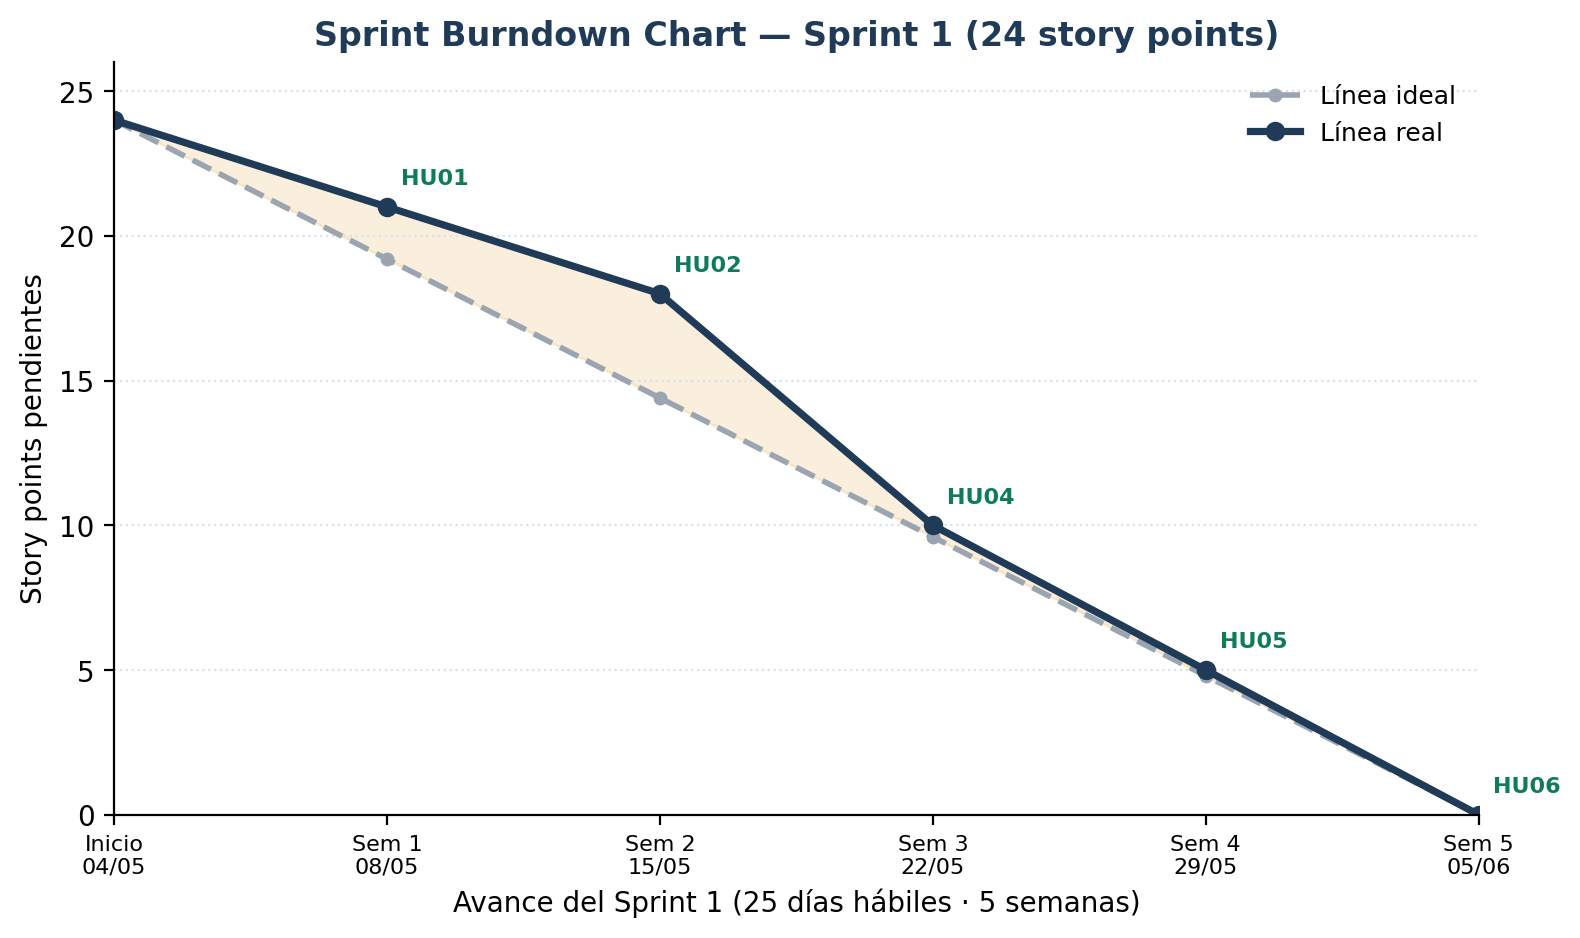
\includegraphics[width=6.5in,height=3.85417in]{figuras/docx_image35.png}

\paragraph{4.1.3.4 Acta de Daily Meeting}\label{acta-de-daily-meeting}

Las actas de reuniones del Sprint 1 deben anexarse como evidencia del
proyecto. Cada acta debe incluir fecha, participantes, avances,
impedimentos, acuerdos y responsables de seguimiento.

\subsubsection{4.1.4 Sprint Review}\label{sprint-review}

El cierre del primer ciclo se formalizó mediante la Sprint Review
realizada al finalizar la semana 8 de iniciada la implementación.
Durante esta sesión, el equipo Scrum presentó el incremento base ante el
Product Owner.

\paragraph{4.1.4.1 Lista de historias de usuario completadas y no
completadas}\label{lista-de-historias-de-usuario-completadas-y-no-completadas}

De acuerdo con la planificación definida para desarrollar las historias
de usuario, se presenta lo siguiente.

\phantomsection\label{_Toc231672291}{}Tabla 36\\
\emph{Estado de Historias de Usuario - Sprint 1}

\begin{longtable}[]{@{}
  >{\raggedright\arraybackslash}p{(\columnwidth - 8\tabcolsep) * \real{0.0944}}
  >{\raggedright\arraybackslash}p{(\columnwidth - 8\tabcolsep) * \real{0.2967}}
  >{\raggedright\arraybackslash}p{(\columnwidth - 8\tabcolsep) * \real{0.1718}}
  >{\raggedright\arraybackslash}p{(\columnwidth - 8\tabcolsep) * \real{0.1942}}
  >{\raggedright\arraybackslash}p{(\columnwidth - 8\tabcolsep) * \real{0.2428}}@{}}
\toprule\noalign{}
\begin{minipage}[b]{\linewidth}\raggedright
\textbf{ID}
\end{minipage} & \begin{minipage}[b]{\linewidth}\raggedright
\textbf{Historia de usuario}
\end{minipage} & \begin{minipage}[b]{\linewidth}\raggedright
\textbf{Estado}
\end{minipage} & \begin{minipage}[b]{\linewidth}\raggedright
\textbf{Entrega Estimada}
\end{minipage} & \begin{minipage}[b]{\linewidth}\raggedright
\textbf{Entrega Real}
\end{minipage} \\
\midrule\noalign{}
\endhead
\bottomrule\noalign{}
\endlastfoot
HU01 & Registro de usuario y empresa & Completado & 25/05/2026 &
29/05/2026 \\
HU02 & Autenticación y roles & Completado & 01/06/2026 & 05/06/2026 \\
HU04 & Ingesta automática de normas & Completado & 04/05/2026 &
08/05/2026 \\
HU05 & Limpieza y normalización textual & Completado & 11/05/2026 &
15/05/2026 \\
HU06 & Vectorización de documentos & Completado & 18/05/2026 &
22/05/2026 \\
\end{longtable}

\paragraph{4.1.4.2 Identificación de problemas presentados en el
sprint}\label{identificaciuxf3n-de-problemas-presentados-en-el-sprint}

A continuación, se describen los principales obstáculos y desafíos
identificados durante la ejecución del Sprint:

\begin{itemize}
\item
  Variabilidad de fuentes normativas: los documentos oficiales pueden
  publicarse en PDF, HTML o formatos con estructura inconsistente.
\item
  Resultado de ingesta sin elementos descubiertos: se requiere
  interpretar correctamente cuándo un rango no contiene documentos y
  cuándo existe un error de extracción.
\item
  Dependencia de configuración de entorno: contenedores, variables,
  rutas de paquete y migraciones deben mantenerse sincronizados.
\item
  Costos potenciales de IA: se determinó que el consumo de OpenAI debe
  reservarse para tareas de generación o evaluación, no para operaciones
  determinísticas del Sprint 1.
\item
  Necesidad de trazabilidad estricta: cada chunk y vector debe
  conectarse con el documento y la URL oficial para evitar respuestas
  sin sustento en Sprint 2.
\end{itemize}

\paragraph{4.1.4.3 Feedback del PO y/o
stakeholders}\label{feedback-del-po-yo-stakeholders}

Tras la revisión del Sprint 1, el Product Owner manifestó conformidad
con el avance del proyecto y validó que la decisión de no depender
obligatoriamente de OpenAI en este primer incremento es coherente con el
objetivo de reducir costos, controlar riesgos y preparar una base
documental verificable. Asimismo, solicitó que en el Sprint 2 las
respuestas del asistente incluyan citaciones oficiales y un mensaje de
advertencia que indique que la respuesta es una orientación operativa y
no asesoría legal vinculante.

\paragraph{4.1.4.4 Acta del Sprint Review}\label{acta-del-sprint-review}

El acta del Sprint Review debe anexarse con la conformidad del
incremento, observaciones del Product Owner, decisiones técnicas
aprobadas y compromisos para el Sprint 2.

\subsubsection{4.1.5 Sprint Retrospective}\label{sprint-retrospective}

La retrospectiva permitió identificar oportunidades de mejora en la
gestión técnica y metodológica del proyecto. La discusión se centró en
la separación entre tareas determinísticas y tareas de IA, la necesidad
de logs detallados y la estandarización del pipeline documental.

\paragraph{4.1.5.1 Plan de acciones de
mejora}\label{plan-de-acciones-de-mejora}

A continuación, se presenta el plan de acciones de mejora para el
Sprint:

\phantomsection\label{_Toc231672292}{}Tabla 37\\
\emph{Plan de acciones de mejora - Sprint 1}

\begin{longtable}[]{@{}
  >{\raggedright\arraybackslash}p{(\columnwidth - 4\tabcolsep) * \real{0.2691}}
  >{\raggedright\arraybackslash}p{(\columnwidth - 4\tabcolsep) * \real{0.3580}}
  >{\raggedright\arraybackslash}p{(\columnwidth - 4\tabcolsep) * \real{0.3729}}@{}}
\toprule\noalign{}
\begin{minipage}[b]{\linewidth}\raggedright
\textbf{¿Qué debemos seguir haciendo?}
\end{minipage} & \begin{minipage}[b]{\linewidth}\raggedright
\textbf{¿Qué debemos empezar a hacer?}
\end{minipage} & \begin{minipage}[b]{\linewidth}\raggedright
\textbf{¿Qué debemos dejar de hacer?}
\end{minipage} \\
\midrule\noalign{}
\endhead
\bottomrule\noalign{}
\endlastfoot
Mantener la revisión técnica del entorno Docker/pytest como parte del
control del sprint. & Verificar la estructura de paquetes, variables
PYTHONPATH y migraciones antes de ejecutar pruebas. & Ejecutar pruebas
sin validar previamente la configuración del entorno. \\
Continuar registrando los resultados del proceso de ingesta normativa. &
Diferenciar en los logs entre ausencia de documentos, error de fuente y
filtros incorrectos. & Interpretar los rangos de ingesta sin resultados
como un único tipo de error. \\
Seguir evaluando distintos formatos documentales dentro del pipeline
normativo. & Ampliar las pruebas con PDF, HTML y Markdown, e incorporar
MarkItDown como herramienta complementaria. & Limitar las pruebas a un
solo formato documental. \\
Mantener la arquitectura flexible para el uso de proveedores de IA. &
Configurar OpenAI como proveedor intercambiable y controlar sus llamadas
mediante variables de entorno. & Depender de un proveedor único o
generar llamadas innecesarias a servicios de IA. \\
Continuar priorizando la trazabilidad de la información normativa. &
Asegurar que cada chunk\_id conserve document\_id, URL, fecha y título
oficial. & Generar fragmentos sin metadatos suficientes para una
citación verificable. \\
\end{longtable}

\paragraph{4.1.5.2 Aprendizaje del sprint}\label{aprendizaje-del-sprint}

A continuación, se detallan las acciones de mejora acordadas durante la
retrospectiva del Sprint 1:

\begin{itemize}
\item
  Se confirmó que separar tareas determinísticas de tareas de IA reduce
  costos y mejora la capacidad de prueba.
\item
  La ingesta normativa requiere logs detallados para diferenciar
  ausencia real de documentos, errores de conexión y filtros mal
  definidos.
\item
  La elección de pgvector simplifica el despliegue inicial al aprovechar
  PostgreSQL como base transaccional y vectorial.
\item
  La normalización textual es crítica porque la calidad de los
  fragmentos condiciona la calidad de las respuestas RAG posteriores.
\item
  Mantener OpenAI configurable, pero no obligatorio en Sprint 1, mejora
  la coherencia entre presupuesto, arquitectura y validación académica.
\end{itemize}

\paragraph{4.1.5.3 Acta del Sprint
Retrospective}\label{acta-del-sprint-retrospective}

La descripción detallada de la retrospectiva debe incorporarse en los
anexos, incluyendo acuerdos, responsables y fechas de seguimiento.

\subsubsection{4.1.6 Refinamiento del Product
Backlog}\label{refinamiento-del-product-backlog}

El refinamiento posterior al Sprint 1 priorizó las historias que
consumen directamente el corpus normativo preparado: configuración de
perfil normativo, consulta en lenguaje natural, respuestas con citas
verificables y contextualización por empresa.

\paragraph{4.1.6.1 Gestión del Product
Backlog}\label{gestiuxf3n-del-product-backlog}

En esta fase, se llevó a cabo un análisis exhaustivo de las Historias de
Usuario. Durante este proceso, se estimó la carga de trabajo requerida
para el cumplimiento del Definition of Done (DoD) de cada ítem.
Asimismo, se seleccionaron estratégicamente las historias con mayor
viabilidad para ser integradas en el Sprint Backlog del segundo ciclo.

\phantomsection\label{_Toc231672293}{}Tabla 38\\
\emph{Gestión Product Backlog - Sprint 2}

\begin{longtable}[]{@{}
  >{\raggedright\arraybackslash}p{(\columnwidth - 10\tabcolsep) * \real{0.0857}}
  >{\raggedright\arraybackslash}p{(\columnwidth - 10\tabcolsep) * \real{0.2628}}
  >{\raggedright\arraybackslash}p{(\columnwidth - 10\tabcolsep) * \real{0.1819}}
  >{\raggedright\arraybackslash}p{(\columnwidth - 10\tabcolsep) * \real{0.1665}}
  >{\raggedright\arraybackslash}p{(\columnwidth - 10\tabcolsep) * \real{0.1363}}
  >{\raggedright\arraybackslash}p{(\columnwidth - 10\tabcolsep) * \real{0.1668}}@{}}
\toprule\noalign{}
\begin{minipage}[b]{\linewidth}\raggedright
\textbf{HU}
\end{minipage} & \begin{minipage}[b]{\linewidth}\raggedright
\textbf{Nombre de la historia de usuario}
\end{minipage} & \begin{minipage}[b]{\linewidth}\raggedright
\textbf{Valor negocio}
\end{minipage} & \begin{minipage}[b]{\linewidth}\raggedright
\textbf{Estimación}
\end{minipage} & \begin{minipage}[b]{\linewidth}\raggedright
\textbf{Método MoSCoW}
\end{minipage} & \begin{minipage}[b]{\linewidth}\raggedright
\textbf{Épica}
\end{minipage} \\
\midrule\noalign{}
\endhead
\bottomrule\noalign{}
\endlastfoot
HU03 & Configuración de perfil normativo & 100 & 5 & M & EP02 \\
HU07 & Clasificación normativa & 90 & 5 & M & EP03 \\
HU08 & Consulta en lenguaje natural & 100 & 8 & M & EP03 \\
HU09 & Respuestas con citas verificables & 100 & 8 & M & EP03 \\
HU10 & Consulta contextualizada & 90 & 5 & S & EP04 \\
\end{longtable}

\paragraph{4.1.6.2 Resumen del refinamiento del Product
Backlog}\label{resumen-del-refinamiento-del-product-backlog}

Durante la reunión de refinamiento, el Product Owner solicitó mantener
la prioridad de las historias orientadas a la consulta RAG, debido a que
el Sprint 1 ya dejó preparado el corpus normativo. Además, se acordó
conservar como deuda técnica la mejora progresiva del extractor para
documentos con formatos no estándar y la ampliación de fuentes
normativas distintas a El Peruano.

\paragraph{4.1.6.3 El acta de
Refinamiento}\label{el-acta-de-refinamiento}

El acta de refinamiento debe anexarse con la lista de historias
priorizadas para Sprint 2, criterios revisados, riesgos técnicos y
acuerdos sobre métricas de validación del asistente regulatorio.

\section{5. Capítulo 5: Validación y Resultados del
Proyecto}\label{capuxedtulo-5-validaciuxf3n-y-resultados-del-proyecto}

Este capítulo detalla la evaluación de calidad del producto a lo largo
de los cuatro Sprints, analizando los incrementos y las mejoras
progresivas obtenidas en cada iteración. Se examina el cumplimiento de
los indicadores de rendimiento (KPIs) y los resultados de la validación
final. Estos hallazgos se presentan organizados por ciclo, asegurando su
alineación con los criterios de éxito establecidos para medir tanto la
calidad técnica del software como la evolución funcional del producto.

\subsection{5.1 Calidad del Producto}\label{calidad-del-producto}

\textbf{Calidad del producto Sprint 1}

En este escenario, se examinan las pruebas realizadas durante el Sprint
1, en el que se llevaron a cabo las historias de usuario HU01, HU02,
HU04, HU05 y HU06. La evaluación de calidad se organiza con base en
características de ISO/IEC 25010 relevantes para el incremento
desarrollado.

\phantomsection\label{_Toc231672294}{}Tabla 39\\
\emph{Métricas de calidad ISO/IEC 25010 - Sprint 1}

\begin{longtable}[]{@{}
  >{\raggedright\arraybackslash}p{(\columnwidth - 4\tabcolsep) * \real{0.1945}}
  >{\raggedright\arraybackslash}p{(\columnwidth - 4\tabcolsep) * \real{0.3580}}
  >{\raggedright\arraybackslash}p{(\columnwidth - 4\tabcolsep) * \real{0.4475}}@{}}
\toprule\noalign{}
\begin{minipage}[b]{\linewidth}\raggedright
\textbf{Características}
\end{minipage} & \begin{minipage}[b]{\linewidth}\raggedright
\textbf{Métricas}
\end{minipage} & \begin{minipage}[b]{\linewidth}\raggedright
\textbf{Evidencias}
\end{minipage} \\
\midrule\noalign{}
\endhead
\bottomrule\noalign{}
\endlastfoot
Adecuación funcional & \begin{minipage}[t]{\linewidth}\raggedright
\begin{itemize}
\item
  Índice de aprobación del incremento con Estado 1.
\item
  Cumplimiento integral de criterios DoD.
\item
  Cumplimiento de criterios de aceptación por HU.
\end{itemize}
\end{minipage} & \begin{minipage}[t]{\linewidth}\raggedright
\begin{itemize}
\item
  Las funcionalidades implementadas fueron satisfactorias para el
  usuario líder.
\item
  Las historias HU01, HU02, HU04, HU05 y HU06 fueron cerradas.
\item
  Los criterios de aceptación fueron verificados mediante CP001 a CP005.
\end{itemize}
\end{minipage} \\
Eficiencia de desempeño & \begin{minipage}[t]{\linewidth}\raggedright
\begin{itemize}
\item
  Ejecución de servicios base sin errores críticos.
\item
  Tiempo de respuesta aceptable en autenticación y consulta de estados.
\item
  Jobs de ingesta registrados con duración y estado.
\end{itemize}
\end{minipage} & \begin{minipage}[t]{\linewidth}\raggedright
\begin{itemize}
\item
  El registro, login y consulta de estados respondieron en escenarios de
  prueba local.
\item
  La ingesta conserva logs aun cuando no existan documentos en un rango.
\end{itemize}
\end{minipage} \\
Usabilidad & \begin{minipage}[t]{\linewidth}\raggedright
\begin{itemize}
\item
  Índice de conformidad del usuario con el flujo de registro e ingreso.
\item
  Ausencia de errores de navegación reportados en el incremento.
\end{itemize}
\end{minipage} & \begin{minipage}[t]{\linewidth}\raggedright
\begin{itemize}
\item
  El usuario puede identificar las pantallas principales y comprender el
  flujo de acceso.
\item
  Se validó que los mensajes de confirmación y error sean comprensibles.
\end{itemize}
\end{minipage} \\
Fiabilidad & \begin{minipage}[t]{\linewidth}\raggedright
\begin{itemize}
\item
  Disponibilidad del entorno de desarrollo durante pruebas.
\item
  Control de errores en ingesta, limpieza y vectorización.
\end{itemize}
\end{minipage} & \begin{minipage}[t]{\linewidth}\raggedright
\begin{itemize}
\item
  Los errores de fuente, documento vacío o proveedor no configurado se
  registran sin detener todo el sistema.
\item
  El sistema diferencia pendiente, procesado y error.
\end{itemize}
\end{minipage} \\
Seguridad & \begin{minipage}[t]{\linewidth}\raggedright
\begin{itemize}
\item
  Protección de contraseñas mediante hash.
\item
  Control de rutas protegidas por sesión o token.
\item
  Uso de variables de entorno para secretos.
\end{itemize}
\end{minipage} & \begin{minipage}[t]{\linewidth}\raggedright
\begin{itemize}
\item
  Las credenciales no se almacenan en texto plano.
\item
  El acceso sin sesión es denegado.
\item
  Las llaves de proveedores externos no quedan embebidas en el código.
\end{itemize}
\end{minipage} \\
Mantenibilidad & \begin{minipage}[t]{\linewidth}\raggedright
\begin{itemize}
\item
  Separación del pipeline por componentes.
\item
  Configuración de proveedores.
\item
  Uso de logs y metadatos.
\end{itemize}
\end{minipage} & \begin{minipage}[t]{\linewidth}\raggedright
\begin{itemize}
\item
  La arquitectura permite cambiar proveedor de embeddings.
\item
  pgvector reduce complejidad operativa al integrarse con PostgreSQL.
\item
  Los logs facilitan diagnóstico y auditoría.
\end{itemize}
\end{minipage} \\
\end{longtable}

El resultado muestra que el Sprint 1 cumple su objetivo como incremento
habilitador. Sin embargo, la precisión del motor RAG, el porcentaje de
citaciones correctas y la satisfacción final del usuario frente al
asistente conversacional no deben declararse como totalmente alcanzados
en esta etapa, porque dependen de las historias de consulta y respuesta
previstas para el Sprint 2.

\subsection{5.2 Incremento del producto}\label{incremento-del-producto}

A continuación, se presentan las evidencias que respaldan el
cumplimiento de cada una de las Historias de Usuario del proyecto,
organizadas de acuerdo con su respectivo incremento de Sprint
correspondiente.

\textbf{Incremento del producto Sprint 1}

El incremento del producto Sprint 1 consolida los componentes necesarios
para que el SIR pase de un diseño arquitectónico a una base operativa de
software. Las evidencias se organizan por historia de usuario y por
resultado entregado.

\begin{itemize}
\item
  Pantallas del incremento del producto
\end{itemize}

\phantomsection\label{_Toc231672434}{}Figura 34\\
\emph{HU01 - Resgistro de usuario y empresa}

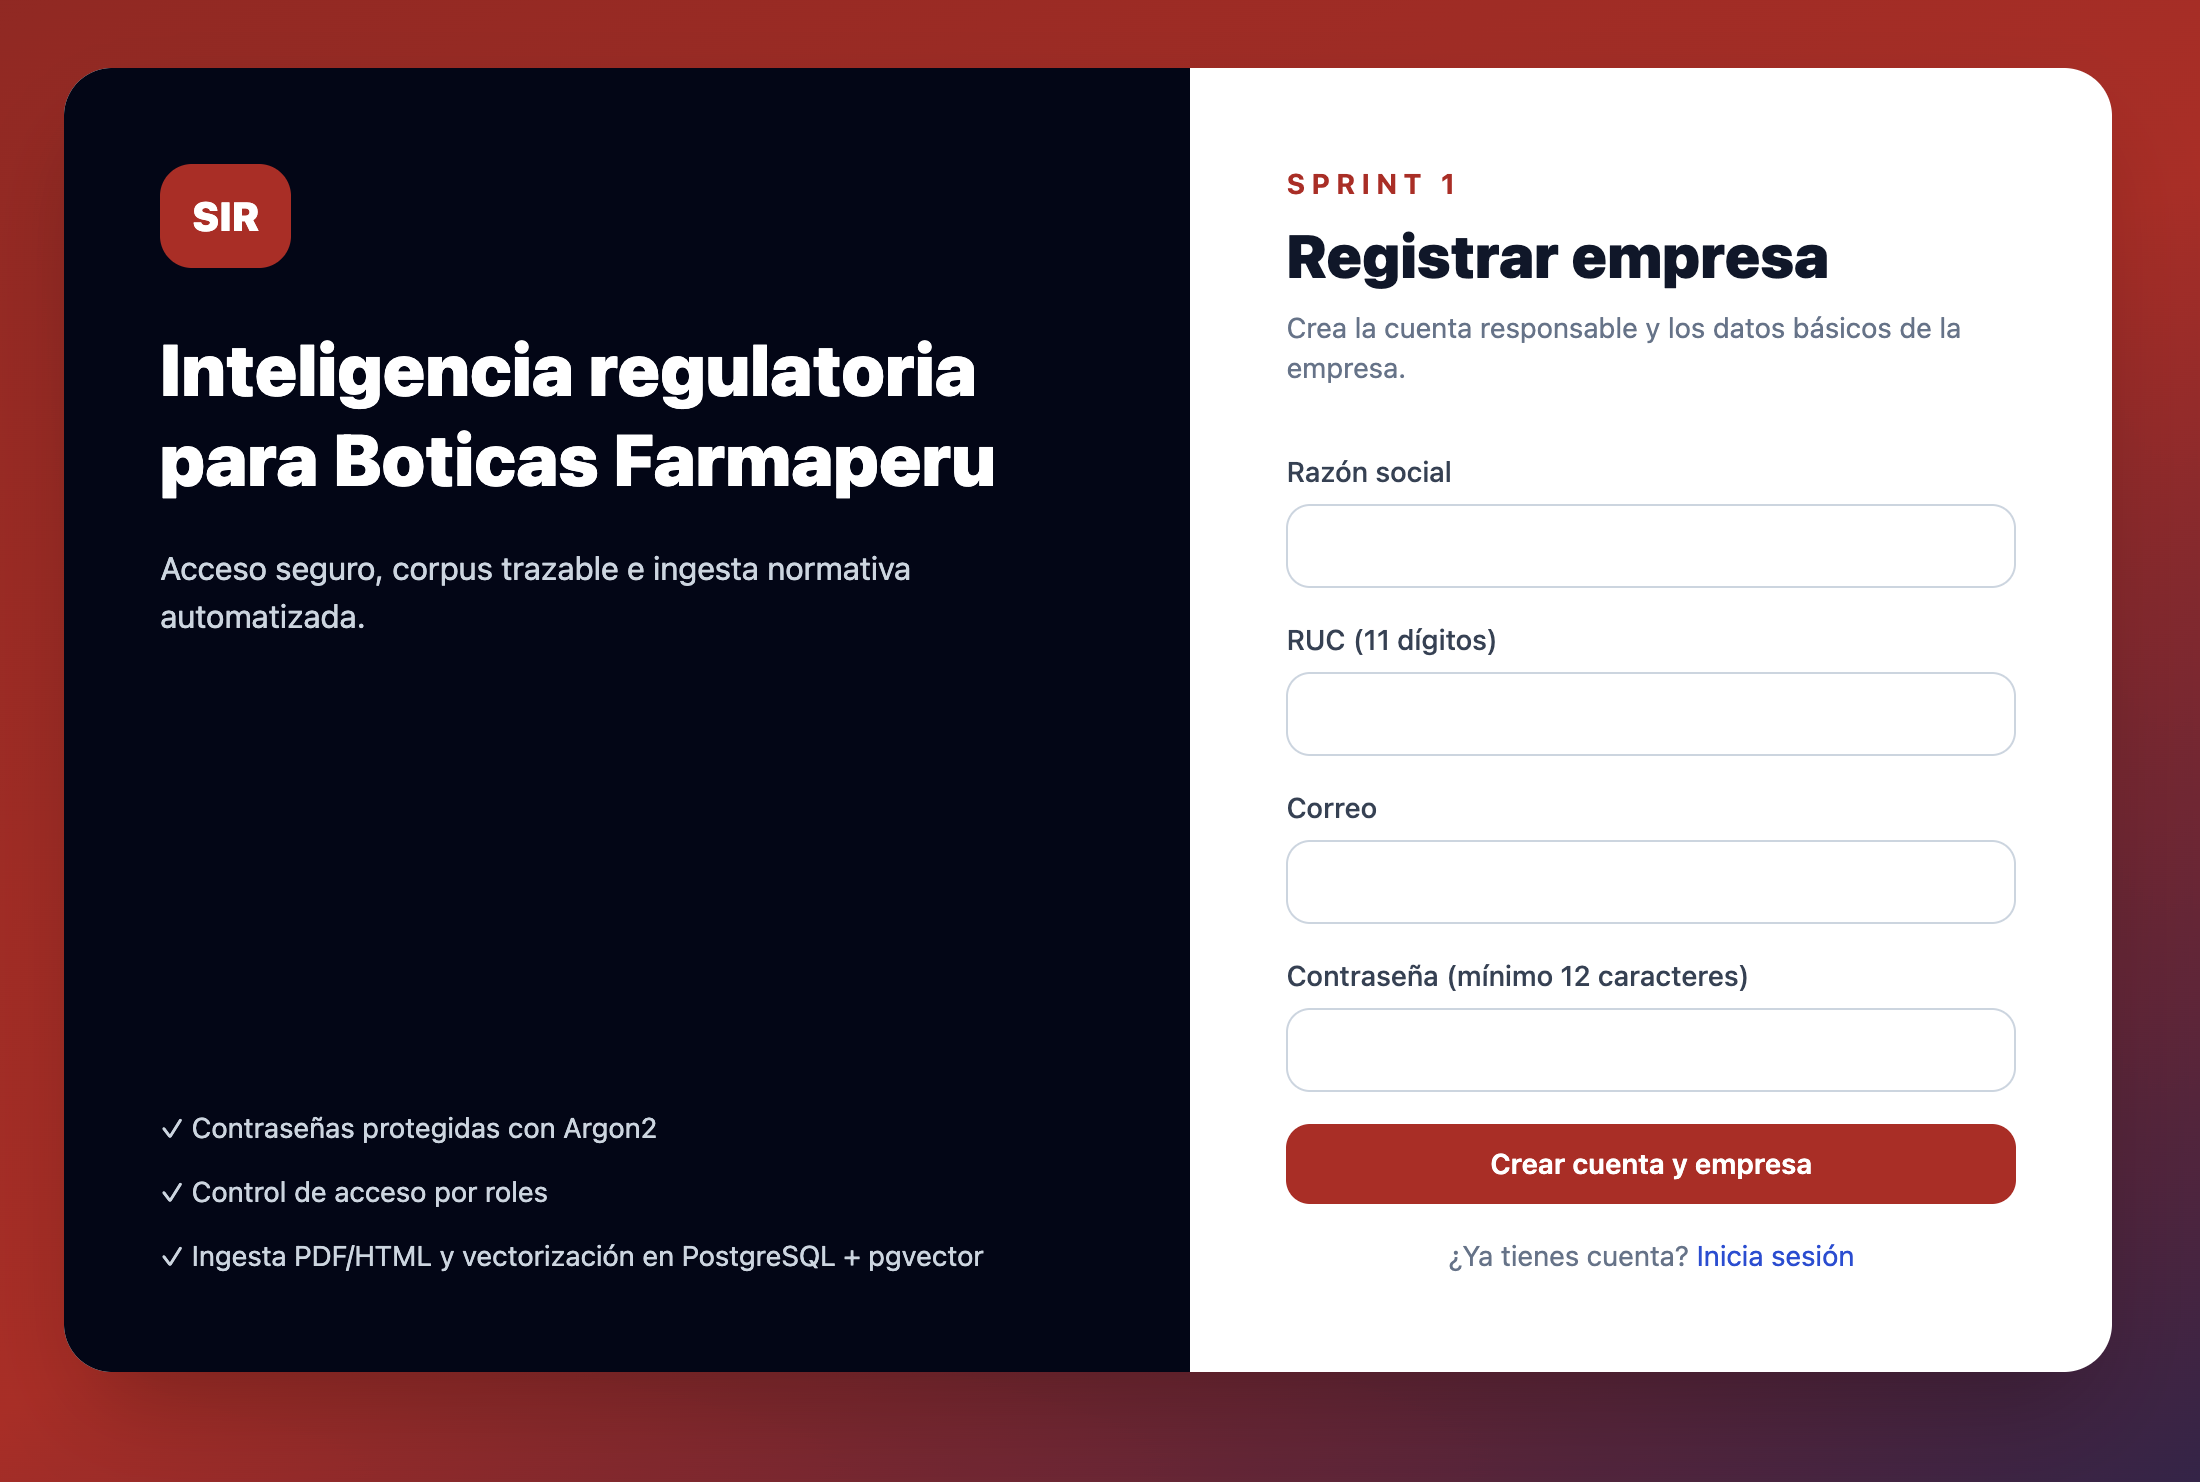
\includegraphics[width=5.59128in,height=3.76635in]{figuras/docx_image29.png}

\phantomsection\label{_Toc231672435}{}Figura 35\\
\emph{HU02 - Autenticación y roles}

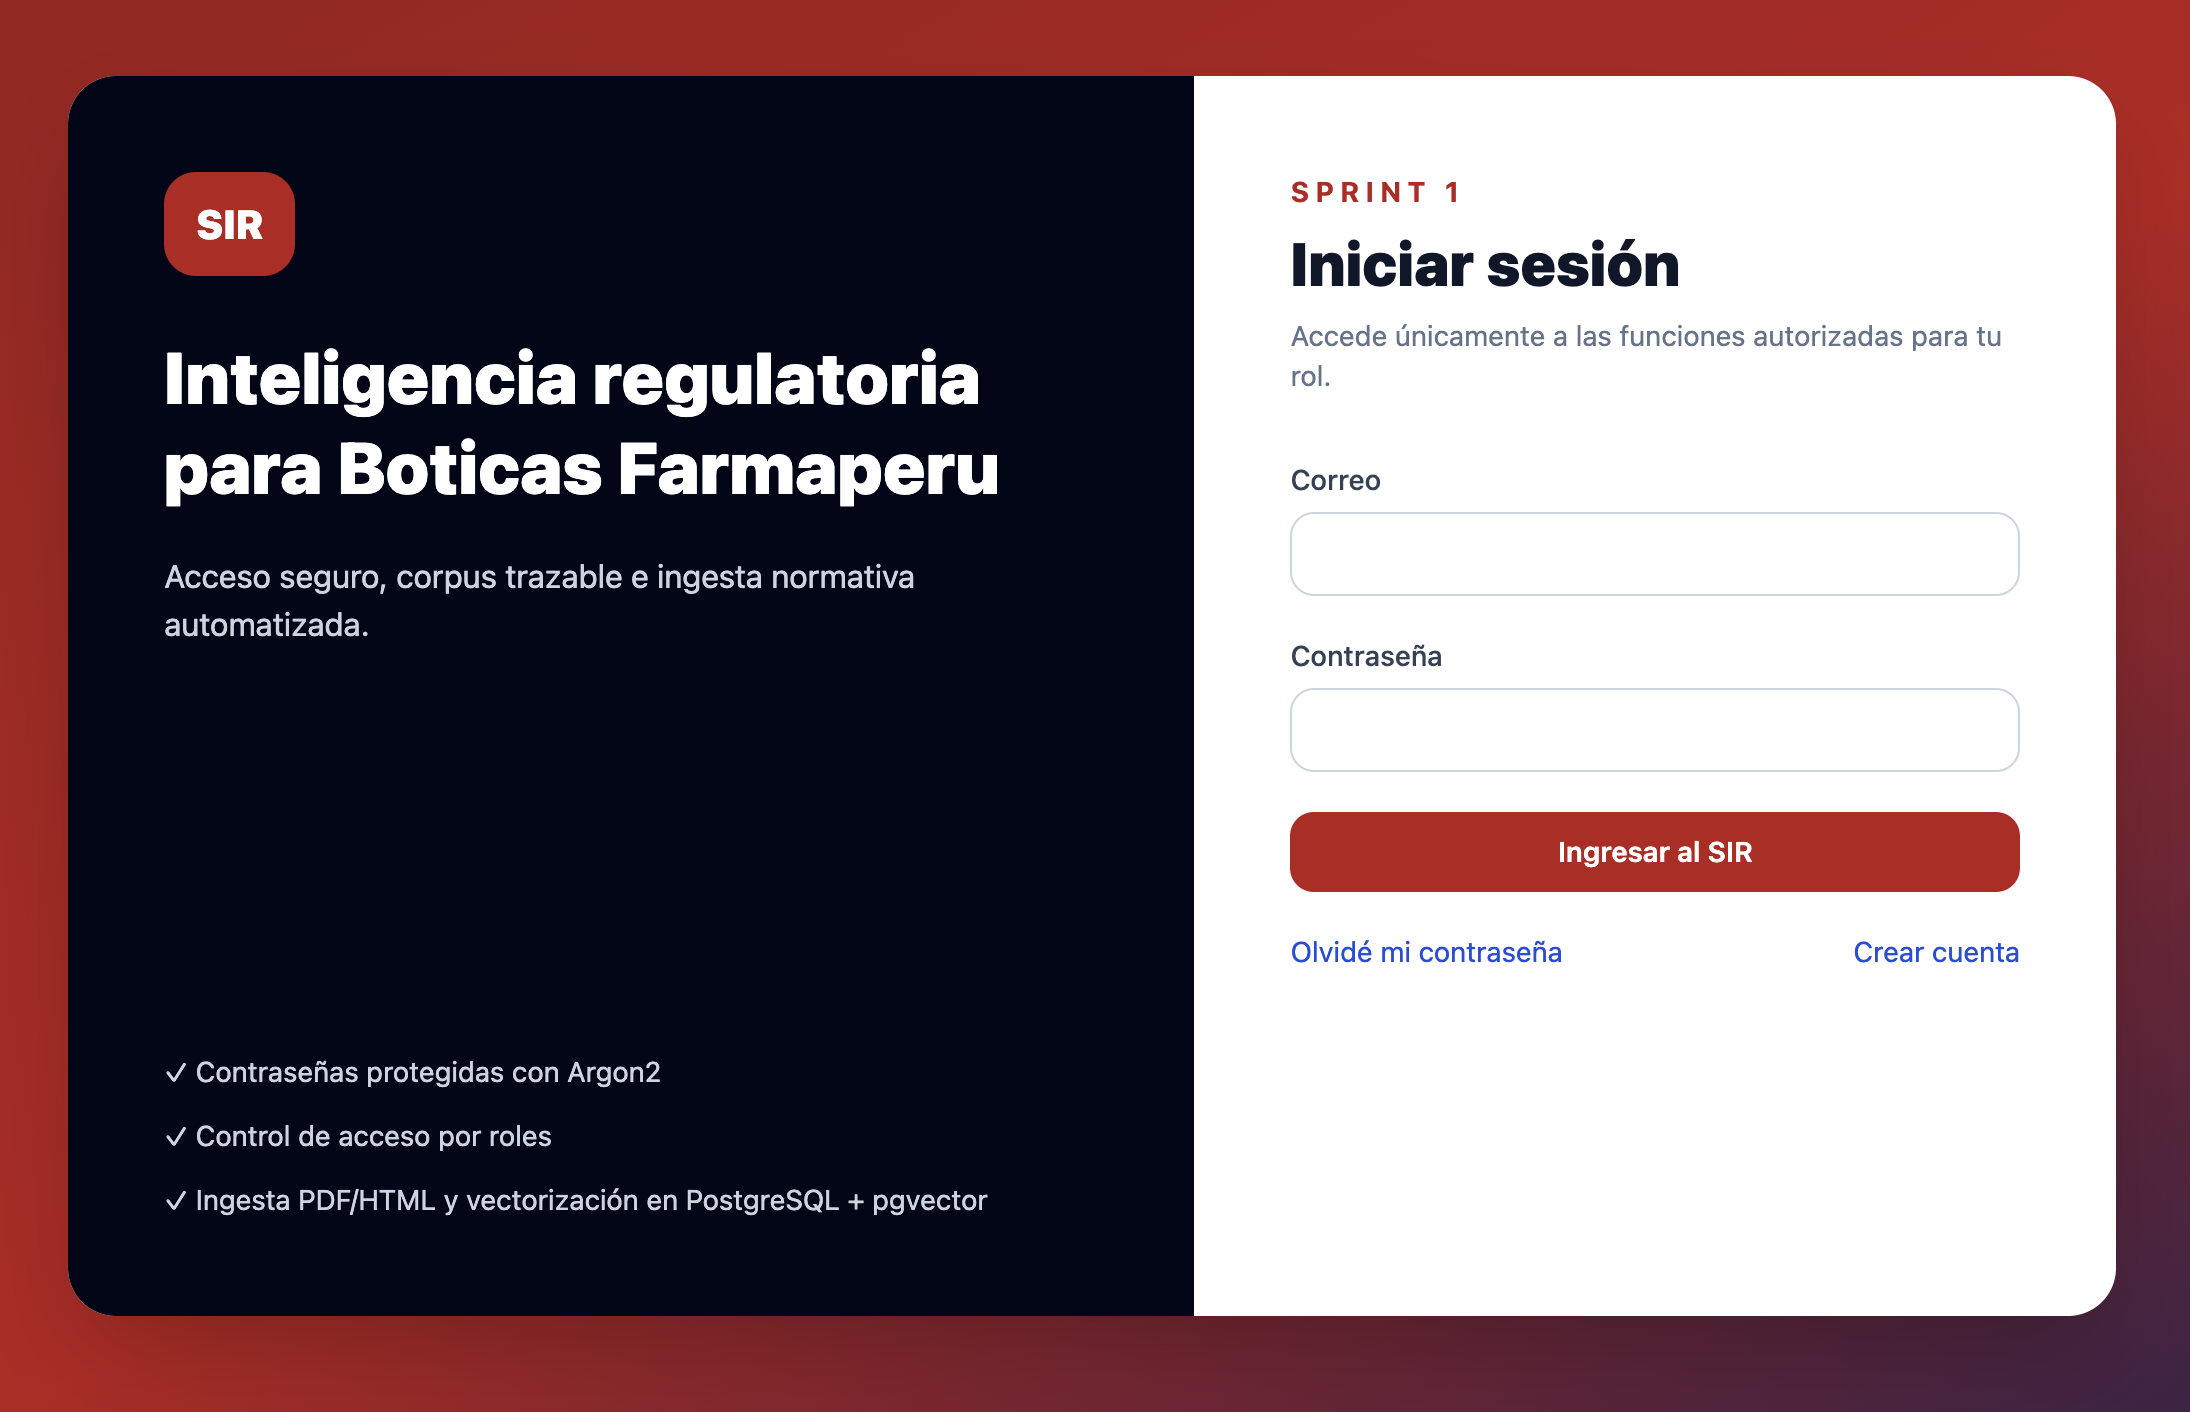
\includegraphics[width=5.58594in,height=3.60162in]{figuras/docx_image30.png}

\phantomsection\label{_Toc231672436}{}Figura 36\\
\emph{HU04 - Ingesta automática de normas}

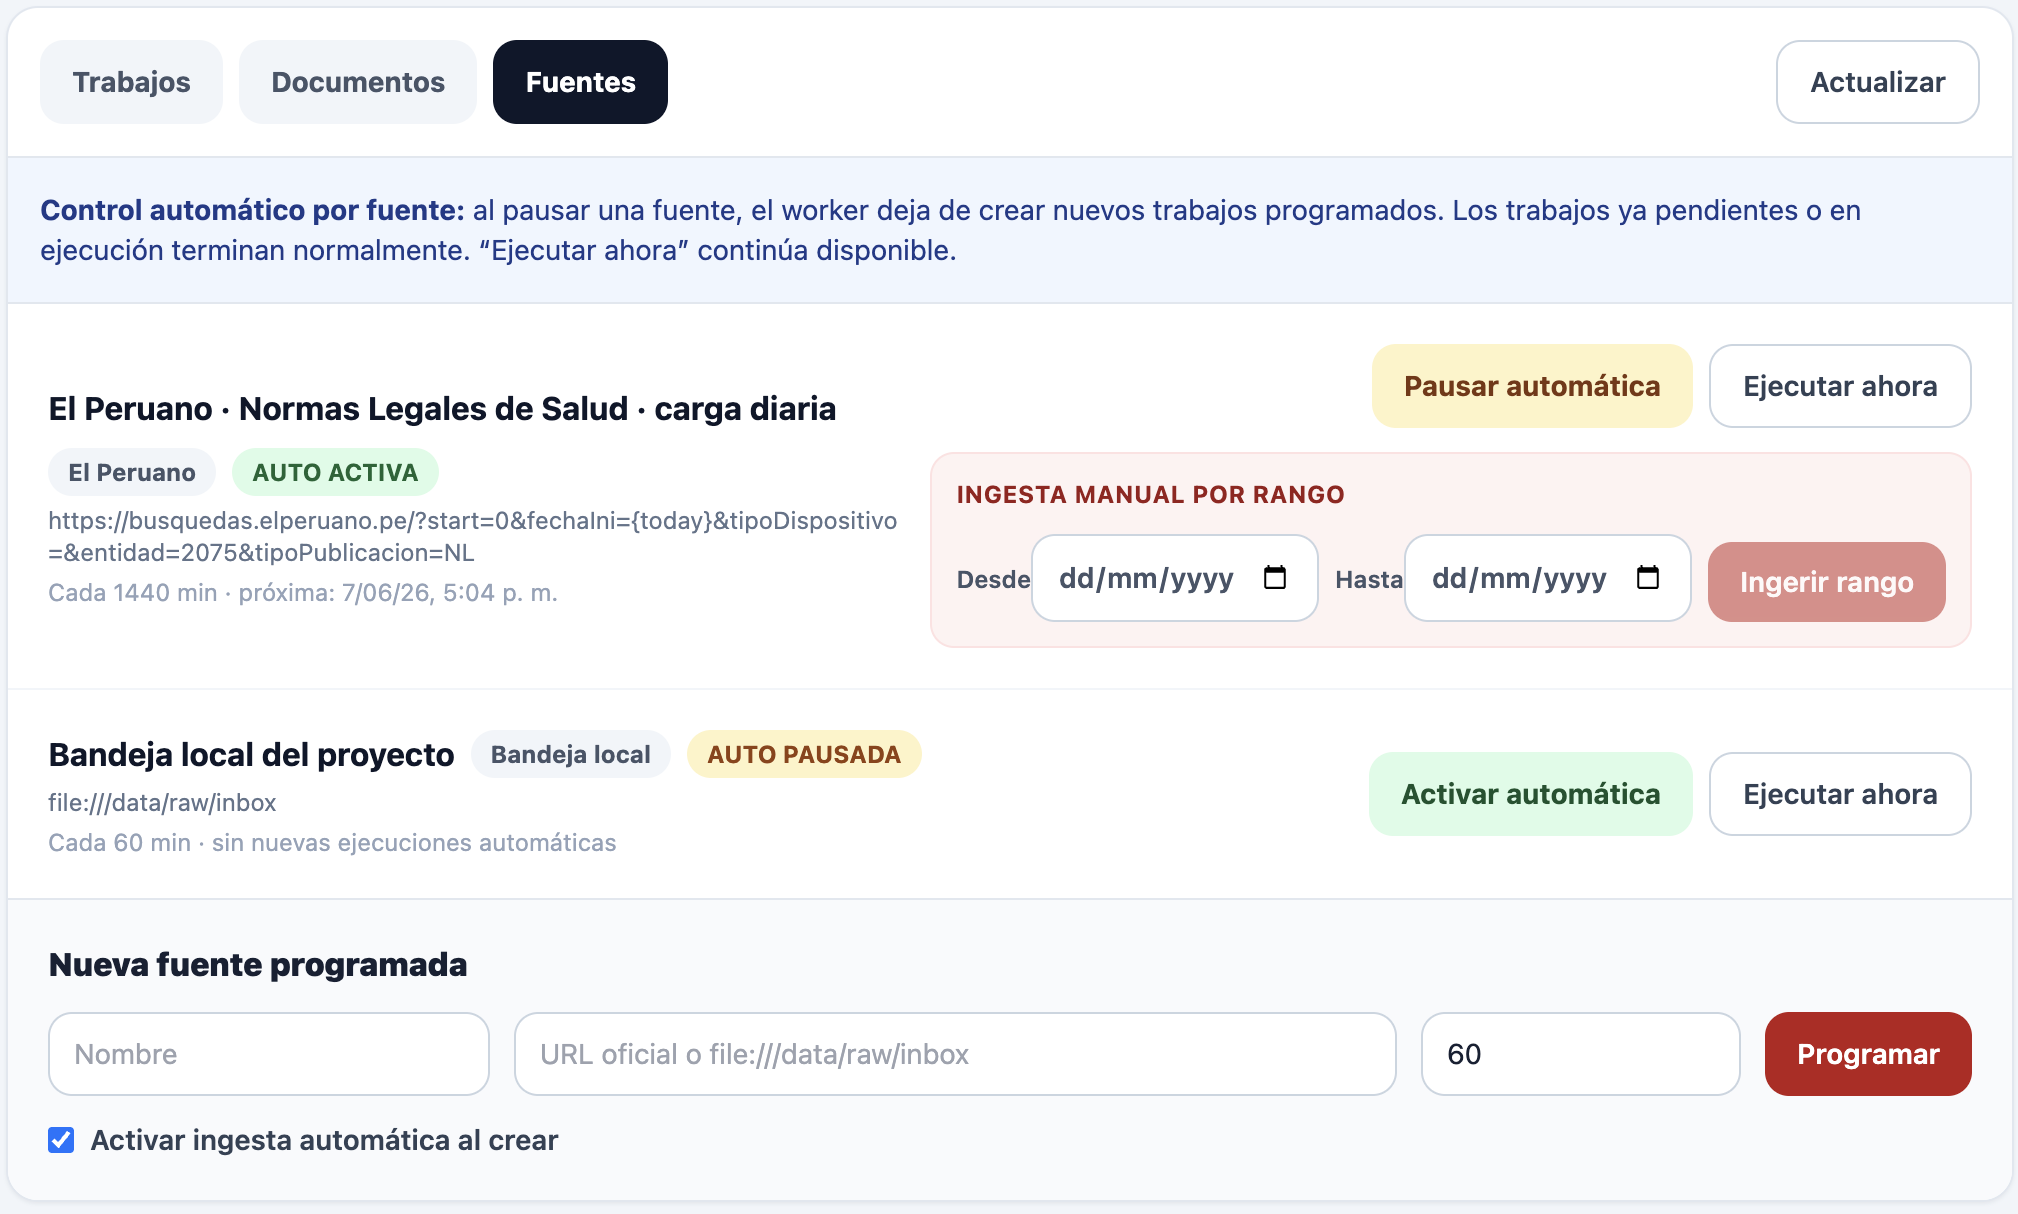
\includegraphics[width=5.58164in,height=3.35793in]{figuras/docx_image31.png}

\phantomsection\label{_Toc231672437}{}Figura 37\\
\emph{HU05 - Limpieza y normalización textual}

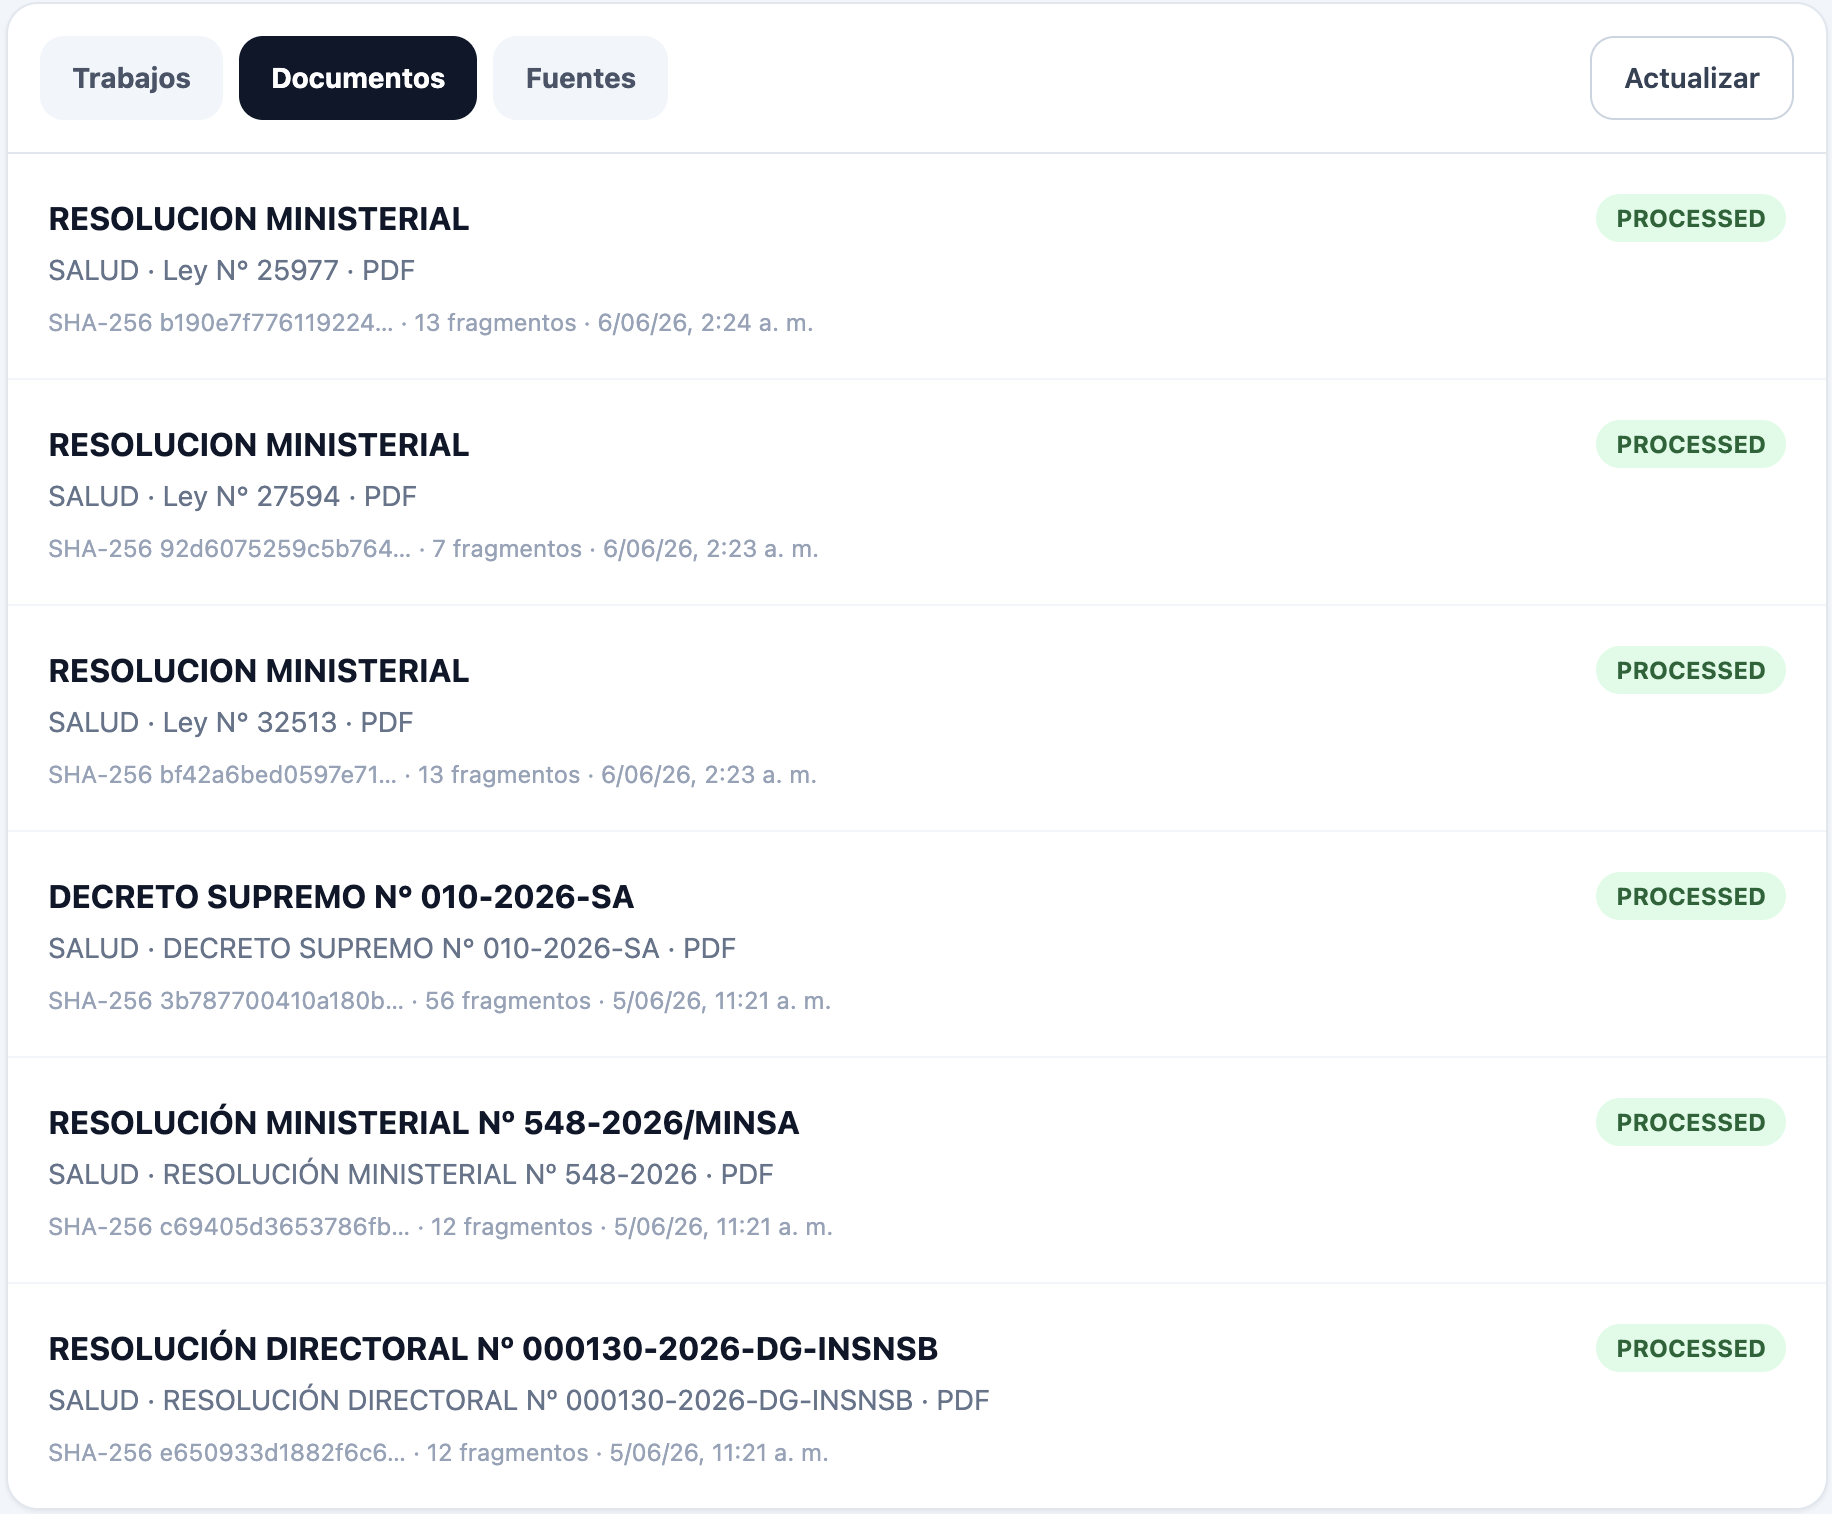
\includegraphics[width=5.58683in,height=3.21474in]{figuras/docx_image32.png}

\phantomsection\label{_Toc231672438}{}Figura 38\\
\emph{HU06 - Vectorización de documentos}

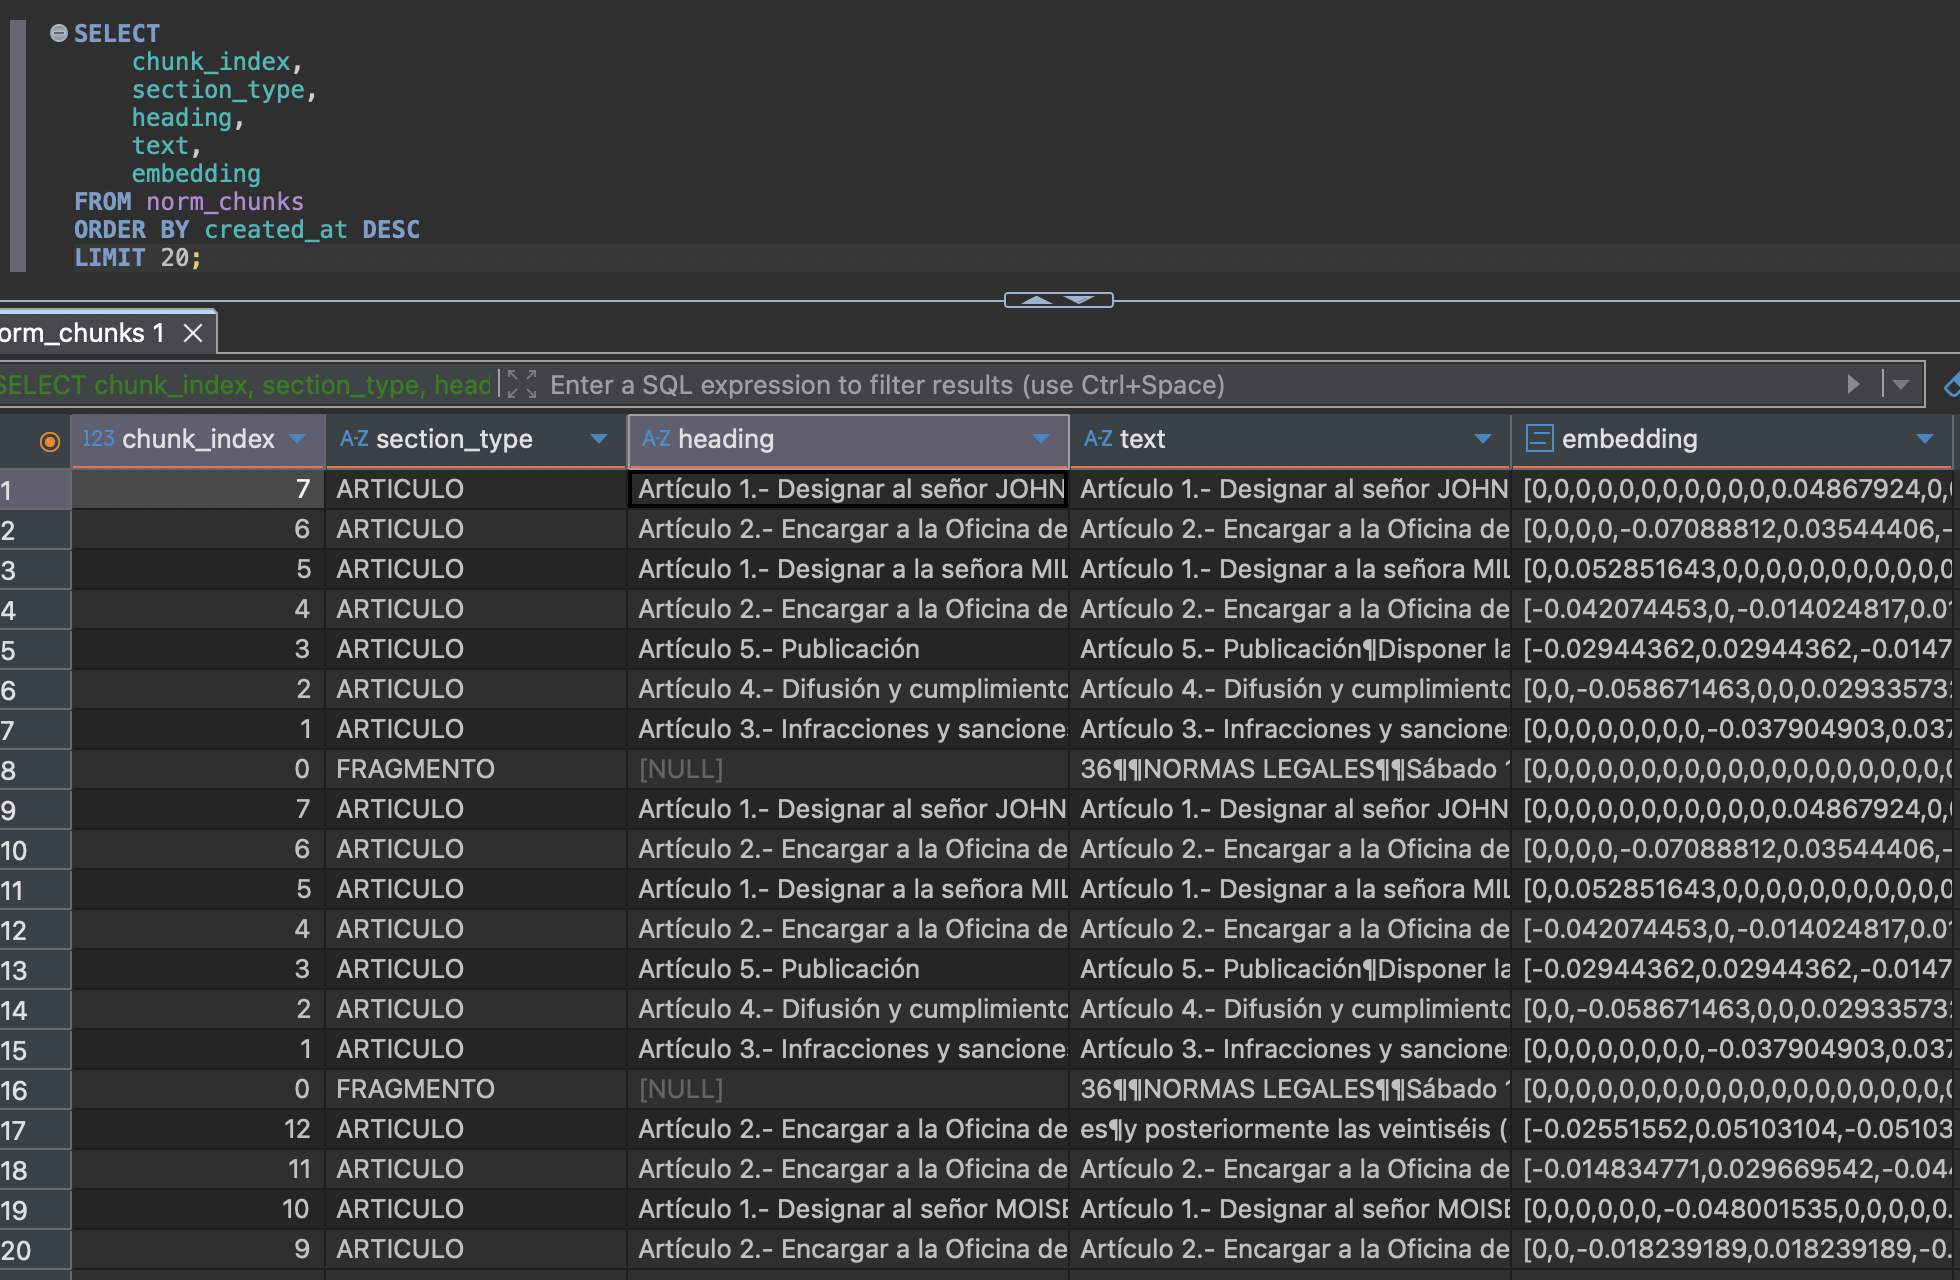
\includegraphics[width=5.91949in,height=3.86601in]{figuras/docx_image33.png}

\begin{itemize}
\item
  Criterios de aceptación
\end{itemize}

\phantomsection\label{_Toc231672295}{}Tabla 40\\
\emph{Criterios de aceptación validados - Sprint 1}

\begin{longtable}[]{@{}
  >{\raggedright\arraybackslash}p{(\columnwidth - 4\tabcolsep) * \real{0.1945}}
  >{\raggedright\arraybackslash}p{(\columnwidth - 4\tabcolsep) * \real{0.3580}}
  >{\raggedright\arraybackslash}p{(\columnwidth - 4\tabcolsep) * \real{0.4475}}@{}}
\toprule\noalign{}
\begin{minipage}[b]{\linewidth}\raggedright
\textbf{ID}
\end{minipage} & \begin{minipage}[b]{\linewidth}\raggedright
\textbf{Historia de Usuario}
\end{minipage} & \begin{minipage}[b]{\linewidth}\raggedright
\textbf{Criterios de Aceptación}
\end{minipage} \\
\midrule\noalign{}
\endhead
\bottomrule\noalign{}
\endlastfoot
HU01 & Registro de usuario y empresa & Los criterios principales fueron
cubiertos mediante pruebas funcionales/técnicas y revisión del
incremento. \\
HU02 & Autenticación y roles & Los criterios principales fueron
cubiertos mediante pruebas funcionales/técnicas y revisión del
incremento. \\
HU04 & Ingesta automática de normas & Los criterios principales fueron
cubiertos mediante pruebas funcionales/técnicas y revisión del
incremento. \\
HU05 & Limpieza y normalización textual & Los criterios principales
fueron cubiertos mediante pruebas funcionales/técnicas y revisión del
incremento. \\
HU06 & Vectorización de documentos & Los criterios principales fueron
cubiertos mediante pruebas funcionales/técnicas y revisión del
incremento. \\
\end{longtable}

\subsection{5.3 Cumplimiento de los indicadores de
éxito}\label{cumplimiento-de-los-indicadores-de-uxe9xito}

En cumplimiento de los indicadores de éxito se presentan los resultados
en concordancia con los objetivos específicos del proyecto.

\subsubsection{Objetivo OE1}\label{objetivo-oe1}

\phantomsection\label{_Toc231672296}{}Tabla 41\\
\emph{Indicadores de éxito OE1}

\begin{longtable}[]{@{}
  >{\raggedright\arraybackslash}p{(\columnwidth - 4\tabcolsep) * \real{0.1945}}
  >{\raggedright\arraybackslash}p{(\columnwidth - 4\tabcolsep) * \real{0.2089}}
  >{\raggedright\arraybackslash}p{(\columnwidth - 4\tabcolsep) * \real{0.5966}}@{}}
\toprule\noalign{}
\begin{minipage}[b]{\linewidth}\raggedright
\textbf{Indicador}
\end{minipage} & \begin{minipage}[b]{\linewidth}\raggedright
\textbf{Estado}
\end{minipage} & \begin{minipage}[b]{\linewidth}\raggedright
\textbf{Evidencia}
\end{minipage} \\
\midrule\noalign{}
\endhead
\bottomrule\noalign{}
\endlastfoot
IE1 Línea base documentada del proceso AS-IS & Cumplido &
\begin{minipage}[t]{\linewidth}\raggedright
\begin{itemize}
\item
  Se cuenta con diagnóstico, línea base y proceso objetivo del
  cumplimiento normativo.
\item
  El Sprint 1 usa esta línea base como referencia para preparar el
  sistema.
\end{itemize}
\end{minipage} \\
Tiempo promedio base de interpretación & Pendiente de comparación &
\begin{minipage}[t]{\linewidth}\raggedright
\begin{itemize}
\item
  Se mantiene el valor base para comparación futura.
\item
  La reducción se medirá cuando el asistente RAG esté operativo.
\end{itemize}
\end{minipage} \\
Trazabilidad inicial de fuentes & Parcialmente cumplido &
\begin{minipage}[t]{\linewidth}\raggedright
\begin{itemize}
\item
  Se define estructura de metadatos y fuente oficial.
\item
  La medición formal de cobertura de citaciones corresponde al Sprint 2.
\end{itemize}
\end{minipage} \\
\end{longtable}

El proyecto cuenta con una línea base suficiente para comparar el
desempeño del SIR en los sprints de validación. Esta línea base será
utilizada para medir reducción de tiempo, exactitud y trazabilidad de
fuentes.

\subsubsection{Objetivo OE2}\label{objetivo-oe2}

\phantomsection\label{_Toc231672297}{}Tabla 42\\
\emph{Indicadores de éxito OE2}

\begin{longtable}[]{@{}
  >{\raggedright\arraybackslash}p{(\columnwidth - 4\tabcolsep) * \real{0.1945}}
  >{\raggedright\arraybackslash}p{(\columnwidth - 4\tabcolsep) * \real{0.2089}}
  >{\raggedright\arraybackslash}p{(\columnwidth - 4\tabcolsep) * \real{0.5966}}@{}}
\toprule\noalign{}
\begin{minipage}[b]{\linewidth}\raggedright
\textbf{Indicador}
\end{minipage} & \begin{minipage}[b]{\linewidth}\raggedright
\textbf{Estado}
\end{minipage} & \begin{minipage}[b]{\linewidth}\raggedright
\textbf{Evidencia}
\end{minipage} \\
\midrule\noalign{}
\endhead
\bottomrule\noalign{}
\endlastfoot
Arquitectura RAG diseñada & Cumplido parcialmente &
\begin{minipage}[t]{\linewidth}\raggedright
\begin{itemize}
\item
  El Sprint 1 implementa componentes de ingesta, normalización, chunking
  y vectorización.
\item
  La generación de respuestas se implementará en Sprint 2.
\end{itemize}
\end{minipage} \\
Corpus normativo trazable & Cumplido &
\begin{minipage}[t]{\linewidth}\raggedright
\begin{itemize}
\item
  Se preparan metadatos de fuente, URL, documento y fragmento.
\item
  La trazabilidad queda lista para citación posterior.
\end{itemize}
\end{minipage} \\
Base vectorial disponible & Cumplido &
\begin{minipage}[t]{\linewidth}\raggedright
\begin{itemize}
\item
  pgvector queda preparado como repositorio semántico.
\item
  Se evita dependencia inicial de servicios vectoriales externos.
\end{itemize}
\end{minipage} \\
\end{longtable}

La arquitectura RAG queda preparada en sus capas de datos y
almacenamiento. La medición formal de citaciones se realizará cuando el
asistente de consulta y respuesta sea incorporado en Sprint 2.

\subsubsection{Objetivo OE3}\label{objetivo-oe3}

\phantomsection\label{_Toc231672298}{}Tabla 43\\
\emph{Indicadores de éxito OE3}

\begin{longtable}[]{@{}
  >{\raggedright\arraybackslash}p{(\columnwidth - 4\tabcolsep) * \real{0.1945}}
  >{\raggedright\arraybackslash}p{(\columnwidth - 4\tabcolsep) * \real{0.2089}}
  >{\raggedright\arraybackslash}p{(\columnwidth - 4\tabcolsep) * \real{0.5966}}@{}}
\toprule\noalign{}
\begin{minipage}[b]{\linewidth}\raggedright
\textbf{Indicador}
\end{minipage} & \begin{minipage}[b]{\linewidth}\raggedright
\textbf{Estado}
\end{minipage} & \begin{minipage}[b]{\linewidth}\raggedright
\textbf{Evidencia}
\end{minipage} \\
\midrule\noalign{}
\endhead
\bottomrule\noalign{}
\endlastfoot
Registro de perfil base & Cumplido &
\begin{minipage}[t]{\linewidth}\raggedright
\begin{itemize}
\item
  HU01 permite asociar usuario y empresa.
\item
  El perfil normativo detallado se completa con HU03.
\end{itemize}
\end{minipage} \\
Acceso seguro & Cumplido & \begin{minipage}[t]{\linewidth}\raggedright
\begin{itemize}
\item
  HU02 habilita autenticación y roles.
\item
  Permite proteger el sistema antes de exponer consultas.
\end{itemize}
\end{minipage} \\
Pipeline normativo & Cumplido &
\begin{minipage}[t]{\linewidth}\raggedright
\begin{itemize}
\item
  HU04, HU05 y HU06 preparan el corpus para recuperación.
\item
  El pipeline queda listo para integración conversacional.
\end{itemize}
\end{minipage} \\
\end{longtable}

El Sprint 1 aporta la infraestructura esencial del SIR. La validación
funcional completa del perfil contextualizado y de las consultas de
usuarios se cerrará en los siguientes sprints.

\subsubsection{Objetivo OE4}\label{objetivo-oe4}

\phantomsection\label{_Toc231672299}{}Tabla 44\\
\emph{Indicadores de éxito OE4}

\begin{longtable}[]{@{}
  >{\raggedright\arraybackslash}p{(\columnwidth - 4\tabcolsep) * \real{0.1945}}
  >{\raggedright\arraybackslash}p{(\columnwidth - 4\tabcolsep) * \real{0.2089}}
  >{\raggedright\arraybackslash}p{(\columnwidth - 4\tabcolsep) * \real{0.5966}}@{}}
\toprule\noalign{}
\begin{minipage}[b]{\linewidth}\raggedright
\textbf{Indicador}
\end{minipage} & \begin{minipage}[b]{\linewidth}\raggedright
\textbf{Estado}
\end{minipage} & \begin{minipage}[b]{\linewidth}\raggedright
\textbf{Evidencia}
\end{minipage} \\
\midrule\noalign{}
\endhead
\bottomrule\noalign{}
\endlastfoot
Precisión de respuestas RAG & Pendiente &
\begin{minipage}[t]{\linewidth}\raggedright
\begin{itemize}
\item
  No aplica todavía.
\item
  Requiere HU08, HU09 y HU10.
\end{itemize}
\end{minipage} \\
Cobertura de citaciones oficiales & Parcial &
\begin{minipage}[t]{\linewidth}\raggedright
\begin{itemize}
\item
  Estructura preparada, medición pendiente.
\item
  Sprint 1 garantiza metadatos; Sprint 2 validará citas en respuestas.
\end{itemize}
\end{minipage} \\
Reducción del tiempo de interpretación & Pendiente &
\begin{minipage}[t]{\linewidth}\raggedright
\begin{itemize}
\item
  No se mide aún.
\item
  Se medirá con casos normativos comparando línea base y uso del SIR.
\end{itemize}
\end{minipage} \\
\end{longtable}

Los indicadores de impacto no deben declararse totalmente alcanzados en
Sprint 1. El valor de este sprint es habilitador: construye la base de
datos, seguridad, ingesta y corpus que harán posible medir precisión,
reducción de tiempo, citación y usabilidad en los siguientes sprints.

\section{7. Capítulo 7: Gestión del
Proyecto}\label{capuxedtulo-7-gestiuxf3n-del-proyecto}

El presente capítulo describe la gestión integral del Sistema de
Inteligencia Regulatoria (SIR) siguiendo el marco PMBOK®, integrado con
la operación ágil descrita en el Capítulo 3. Se documentan los siete
planes de gestión por área de conocimiento (alcance, cronograma, costos,
calidad, riesgos, comunicaciones e interesados), así como la ejecución y
el monitoreo durante los ciclos académicos PI-1 y PI-2 y las lecciones
aprendidas del proyecto. Todos los artefactos guardan correspondencia
con el caso de estudio (Inversiones y Representaciones Peruanas LK
S.R.L. -- Boticas Farmaperu).

\textbf{Definición del proyecto y participantes}

\phantomsection\label{_Toc231672300}{}Tabla 45\\
\emph{Definición del proyecto y participantes}

\begin{longtable}[]{@{}
  >{\raggedright\arraybackslash}p{(\columnwidth - 4\tabcolsep) * \real{0.2533}}
  >{\raggedright\arraybackslash}p{(\columnwidth - 4\tabcolsep) * \real{0.2835}}
  >{\raggedright\arraybackslash}p{(\columnwidth - 4\tabcolsep) * \real{0.4632}}@{}}
\toprule\noalign{}
\begin{minipage}[b]{\linewidth}\raggedright
Código Proyecto
\end{minipage} &
\multicolumn{2}{>{\raggedright\arraybackslash}p{(\columnwidth - 4\tabcolsep) * \real{0.7467} + 2\tabcolsep}@{}}{%
\begin{minipage}[b]{\linewidth}\raggedright
Descripción General
\end{minipage}} \\
\midrule\noalign{}
\endhead
\bottomrule\noalign{}
\endlastfoot
SIR-2026-04 &
\multicolumn{2}{>{\raggedright\arraybackslash}p{(\columnwidth - 4\tabcolsep) * \real{0.7467} + 2\tabcolsep}@{}}{%
Sistema de Inteligencia Regulatoria basado en IA generativa con
arquitectura RAG para automatizar la interpretación de normas legales en
una PYME farmacéutica minorista del Perú (Boticas Farmaperu). Equipo de
2 estudiantes; horizonte de 32 semanas en 4 sprints distribuidos en PI-1
y PI-2.} \\
\textbf{Rol} & \textbf{Nombre de participante} &
\textbf{Responsabilidades principales} \\
Jefe de Proyecto & Mogollón Buitrón, Khail & Planificar, ejecutar y
controlar el proyecto. Gestionar alcance, cronograma, costos, riesgos y
comunicaciones. \\
Product Owner & Quispe Rojas, Ana María (rep. PYME) & Priorizar el
Product Backlog desde la perspectiva del negocio farmacéutico, validar
el valor de cada incremento. \\
Scrum Master & Hervias Salas, Jadir & Facilitar ceremonias Scrum,
eliminar impedimentos, asegurar el cumplimiento del marco ágil. \\
Líder Técnico & Hervias Salas, Jadir & Definir y mantener la
arquitectura técnica (C4, RAG, BD). \\
Analista Funcional & Mogollón Buitrón, Khail & Levantar requerimientos,
modelar HUs y criterios SMART. \\
Desarrollador Backend / IA & Hervias Salas, Jadir & Implementar API,
ingesta normativa, embeddings y motor RAG. \\
Desarrollador Frontend & Mogollón Buitrón, Khail & Implementar
interfaces de perfil, asistente, dashboard, alertas, calendario,
evidencias y reportes. \\
Analista QA & Equipo de desarrollo & Diseñar y ejecutar pruebas
funcionales, de IA, usabilidad y rendimiento. \\
Asesor & Zacarías Ramos, Juan & Asesorar y validar avances del primer
ciclo académico. \\
Sponsor / Cliente & Gerencia de Boticas Farmaperu & Aprobar alcance
funcional, facilitar acceso a información operativa y validar la
utilidad del sistema. \\
Usuario Líder & Responsable administrativo de Boticas Farmaperu &
Validar prototipos, aplicar SUS y participar en el experimento de
comprensión normativa. \\
\end{longtable}

\subsection{7.1 Planificación del
Proyecto}\label{planificaciuxf3n-del-proyecto}

\subsubsection{7.1.1 Plan de Gestión del
Alcance}\label{plan-de-gestiuxf3n-del-alcance}

\paragraph{7.1.1.1 Consideraciones de gestión del
alcance}\label{consideraciones-de-gestiuxf3n-del-alcance}

\phantomsection\label{_Toc231672301}{}Tabla 46\\
\emph{Entregables principales del proyecto}

\begin{longtable}[]{@{}
  >{\raggedright\arraybackslash}p{(\columnwidth - 4\tabcolsep) * \real{0.0746}}
  >{\raggedright\arraybackslash}p{(\columnwidth - 4\tabcolsep) * \real{0.3731}}
  >{\raggedright\arraybackslash}p{(\columnwidth - 4\tabcolsep) * \real{0.5522}}@{}}
\toprule\noalign{}
\multicolumn{3}{@{}>{\raggedright\arraybackslash}p{(\columnwidth - 4\tabcolsep) * \real{1.0000} + 4\tabcolsep}@{}}{%
\begin{minipage}[b]{\linewidth}\raggedright
DESCRIPCIÓN DEL PRODUCTO DEL PROYECTO (Características, funcionalidades,
requisitos, soporte, entre otros)
\end{minipage}} \\
\midrule\noalign{}
\endhead
\bottomrule\noalign{}
\endlastfoot
\multicolumn{3}{@{}>{\raggedright\arraybackslash}p{(\columnwidth - 4\tabcolsep) * \real{1.0000} + 4\tabcolsep}@{}}{%
El Sistema de Inteligencia Regulatoria (SIR) es una plataforma web que
aplica IA generativa con arquitectura Retrieval-Augmented Generation
(RAG) sobre el corpus normativo del Diario Oficial El Peruano y de las
entidades reguladoras relevantes para una PYME farmacéutica minorista
(DIGEMID/MINSA, SUNAT, SUNAFIL, INDECOPI y municipalidad). El producto
integra perfil empresarial, repositorio normativo, asistente regulatorio
con IA, dashboard de cumplimiento, matriz de obligaciones, calendario de
vencimientos, sistema básico de alertas, generación de reportes,
repositorio de evidencias, historial, auditoría, retroalimentación y
administración de usuarios.} \\
\multicolumn{3}{@{}>{\raggedright\arraybackslash}p{(\columnwidth - 4\tabcolsep) * \real{1.0000} + 4\tabcolsep}@{}}{%
\textbf{DESCRIPCIÓN DE ENTREGABLES PRINCIPALES DEL PROYECTO}} \\
\textbf{Nro.} & \textbf{DESCRIPCIÓN} & \textbf{CRITERIOS DE
ACEPTACIÓN} \\
1 & Memoria de investigación & Documento de tesis aprobado por el asesor
con índice de similitud \textless{} 20\%. \\
2 & Pipeline de ingesta normativa & Extracción diaria automatizada del
Diario Oficial El Peruano y portales DIGEMID/SUNAT; logs y métricas
operativas. \\
3 & Plataforma SIR (frontend + backend + RAG) & Sistema desplegado,
login operativo, asistente con citas verificables, dashboard, matriz de
obligaciones, alertas, calendario, reportes y evidencias. \\
4 & Documentación de arquitectura (modelo C4 + 4+1) & Diagramas
Conceptual, Físico, Lógico, Contexto, Contenedores y Componentes en
draw.io aprobados. \\
5 & Plan de pruebas y reportes de validación & Pruebas unitarias ≥ 80\%
cobertura; pruebas de IA F1 ≥ 0.85; SUS ≥ 75. \\
6 & Material de presentación final por ciclo & Demo funcional para PI-1
y PI-2; sustentación aprobada. \\
\end{longtable}

\phantomsection\label{_Toc231672302}{}Tabla 47\\
\emph{Exclusiones, restricciones y supuestos del proyecto}

\begin{longtable}[]{@{}
  >{\raggedright\arraybackslash}p{(\columnwidth - 0\tabcolsep) * \real{1.0000}}@{}}
\toprule\noalign{}
\begin{minipage}[b]{\linewidth}\raggedright
EXCLUSIONES DEL PROYECTO (Entregables no considerados como parte del
proyecto)
\end{minipage} \\
\midrule\noalign{}
\endhead
\bottomrule\noalign{}
\endlastfoot
\begin{minipage}[t]{\linewidth}\raggedright
\begin{itemize}
\item
  Asesoría legal vinculante o emisión de opinión jurídica formal.
\item
  Integración con sistemas internos de la PYME (ERP, contabilidad,
  facturación electrónica).
\item
  Ejecución directa de declaraciones tributarias, trámites o
  presentación de documentos ante entidades públicas.
\item
  Cobertura de jurisprudencia y doctrina (alcance limitado a normativa
  publicada).
\item
  Aplicación móvil nativa (solo aplicación web responsive).
\end{itemize}
\end{minipage} \\
\textbf{RESTRICCIONES} (Límites de recursos en términos de tiempo,
costos, infraestructura u otros, sean internas o externas, que puede
afectar al rendimiento del proyecto) \\
\begin{minipage}[t]{\linewidth}\raggedright
\begin{itemize}
\item
  Equipo: dos estudiantes con dedicación parcial.
\item
  Tiempo: 32 semanas distribuidas en cuatro sprints en dos ciclos
  académicos (PI-1 y PI-2).
\item
  Presupuesto: limitado a planes free-tier de servicios cloud y créditos
  académicos de OpenAI.
\item
  Tecnología: dependencia de la disponibilidad pública del Diario
  Oficial El Peruano y de las APIs de OpenAI, Pinecone y SendGrid.
\item
  Legal: cumplimiento de Ley N.º 29733 (datos personales) y Ley N.º
  31814 (Inteligencia Artificial).
\end{itemize}
\end{minipage} \\
\textbf{SUPUESTOS} (Factores que, para efectos de planificación, se
consideran verdaderas, reales o ciertas sin necesidad de pruebas o
demostraciones) \\
\begin{minipage}[t]{\linewidth}\raggedright
\begin{itemize}
\item
  El Diario Oficial El Peruano y los portales DIGEMID/MINSA mantienen su
  acceso público durante los 8 meses del proyecto.
\item
  OpenAI mantiene disponibilidad y precios compatibles con los créditos
  académicos.
\item
  Boticas Farmaperu mantiene su disponibilidad para validar entregables
  y participar en el experimento de comprensión normativa.
\item
  Los asesores de mantienen su disponibilidad para las asesorías
  quincenales.
\end{itemize}
\end{minipage} \\
\end{longtable}

\paragraph{7.1.1.2 Línea Base del
Alcance}\label{luxednea-base-del-alcance}

Se presenta el Estructura de Desglose del Trabajo (EDT) del proyecto
conformado por las fases de Inicio, Planificación, Ejecución,
Seguimiento y Monitoreo, y Cierre. La visualización completa del EDT y
el diccionario detallado de los paquetes de tercer y cuarto nivel se
incluyen en el Anexo del documento.

\phantomsection\label{_Toc231672439}{}Figura\\
\emph{Estructura de desglose de trabajo (EDT)}

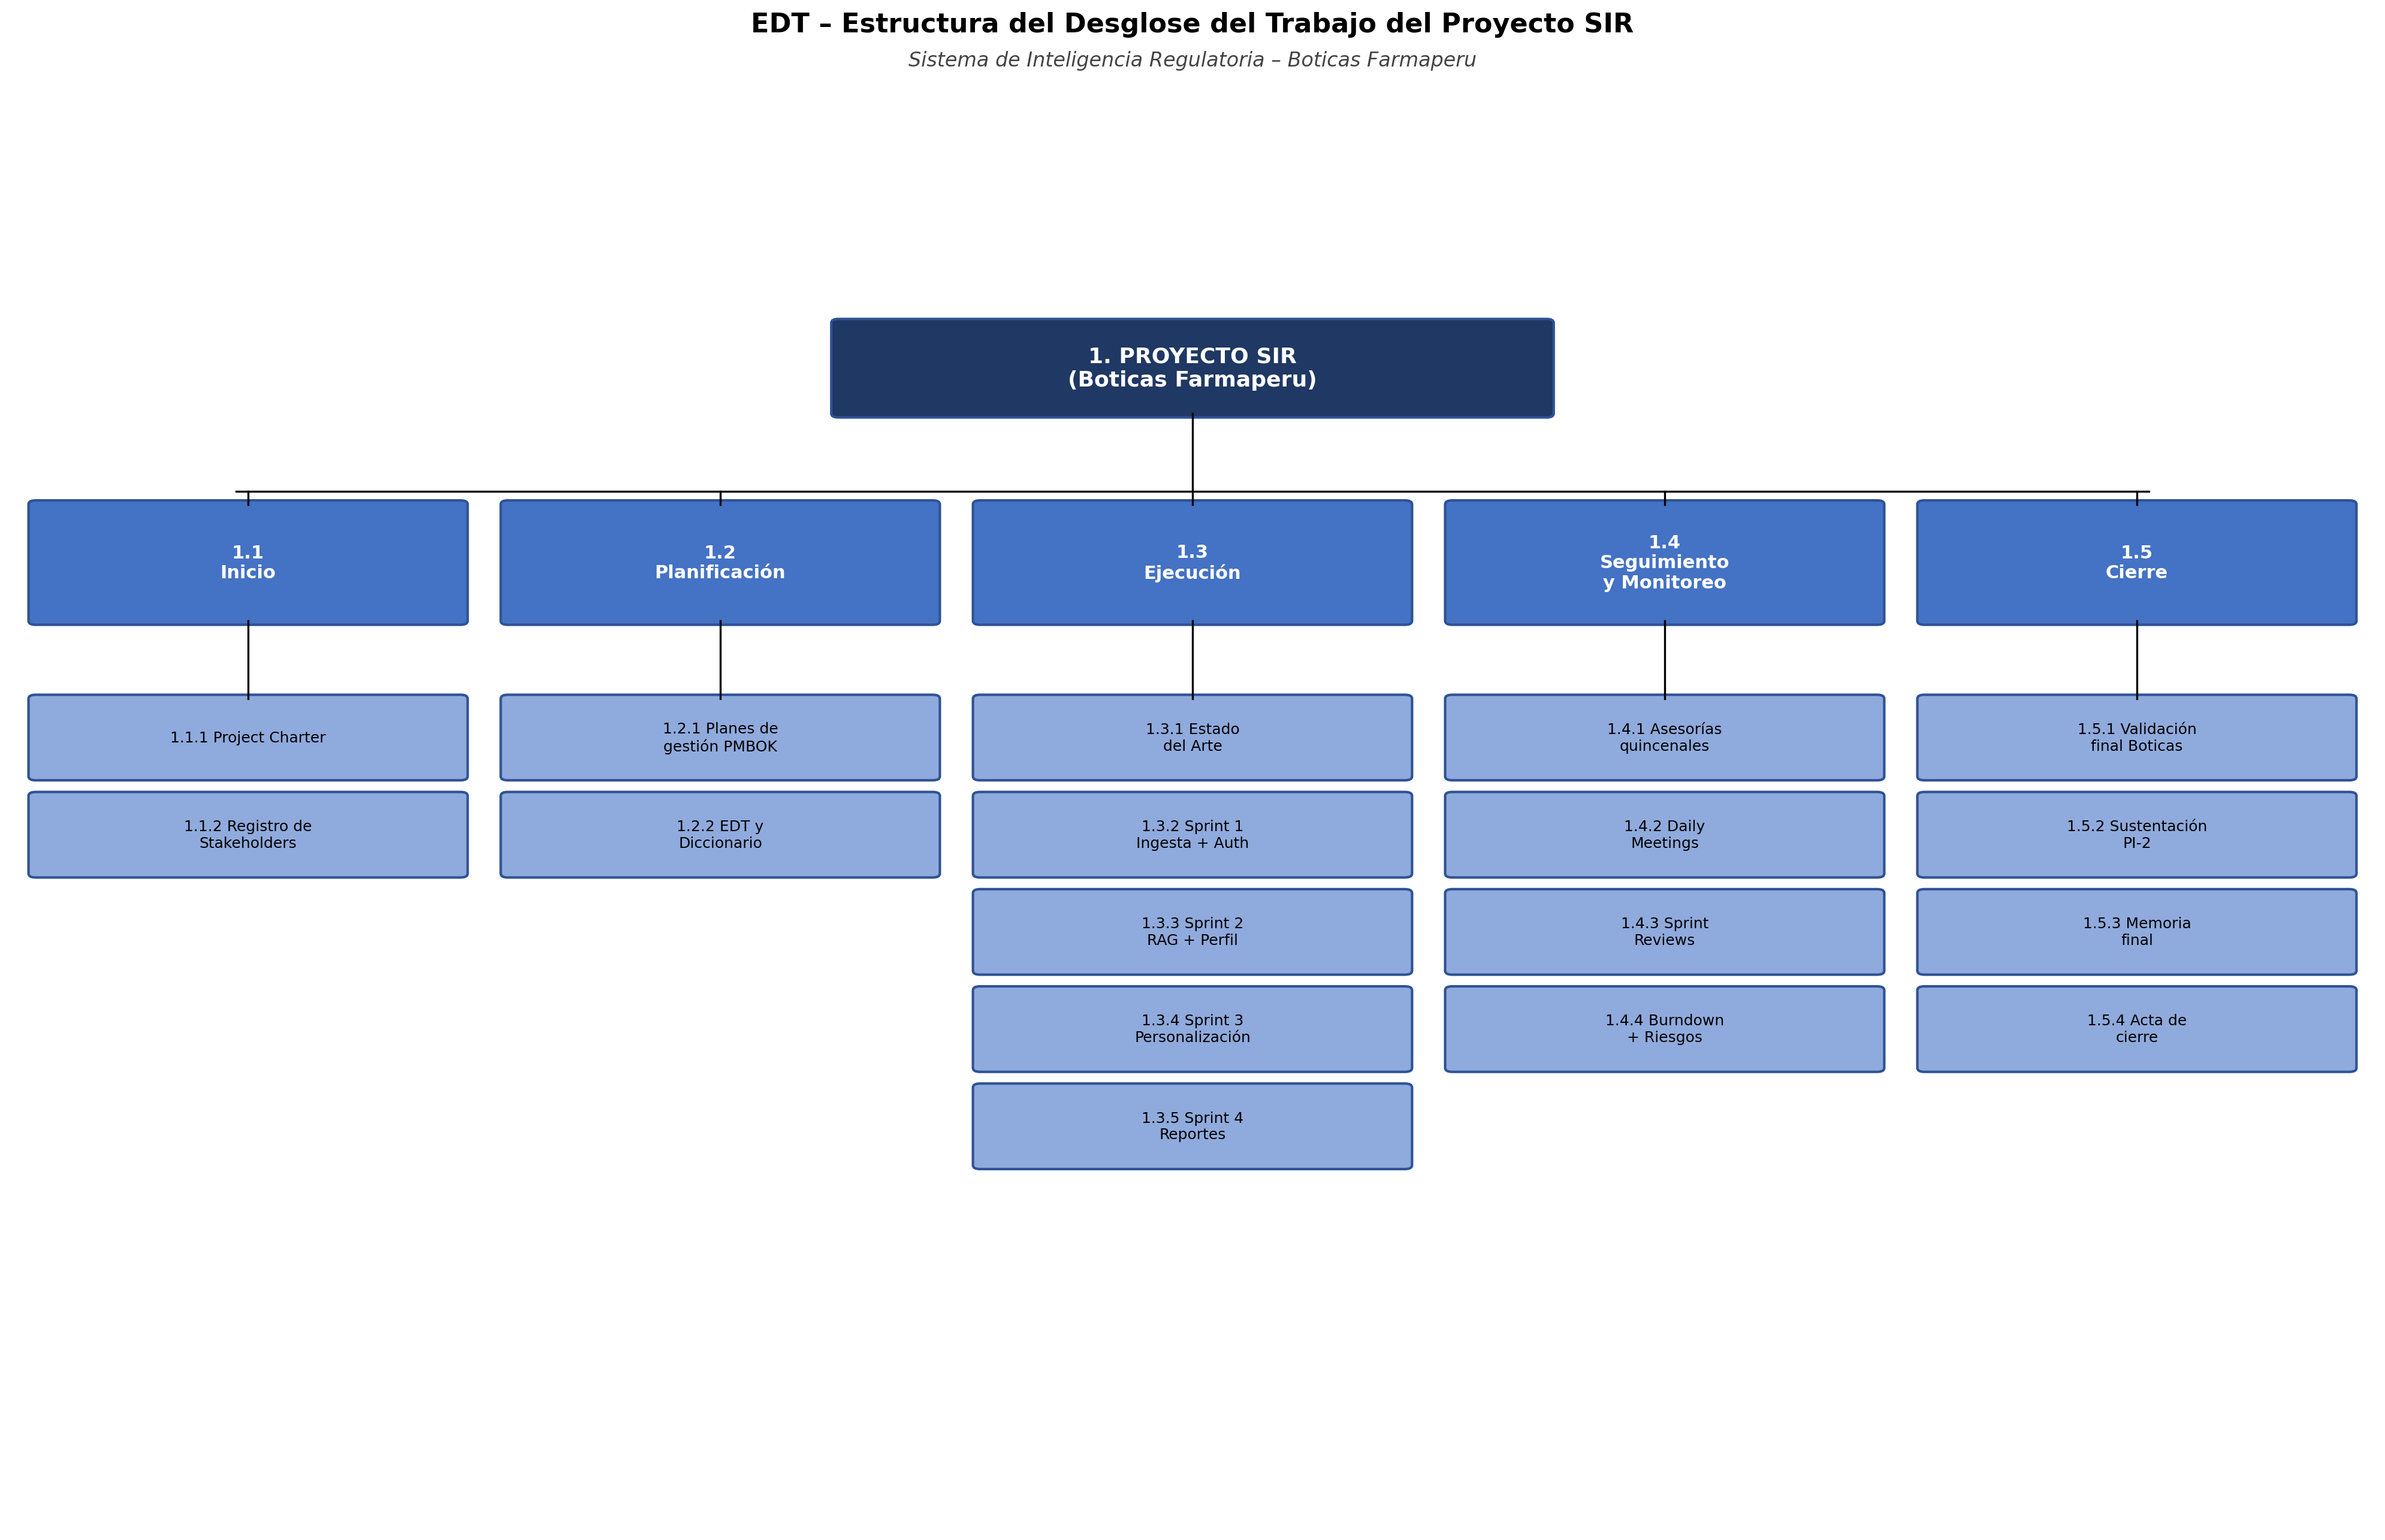
\includegraphics[width=5.90163in,height=2.54653in]{figuras/docx_image36.png}

\textbf{EDT - Diccionario (paquetes de trabajo principales):}

\phantomsection\label{_Toc231672303}{}Tabla 48\\
\emph{Diccionario EDT - paquetes de trabajo principales}

\begin{longtable}[]{@{}
  >{\raggedright\arraybackslash}p{(\columnwidth - 8\tabcolsep) * \real{0.1113}}
  >{\raggedright\arraybackslash}p{(\columnwidth - 8\tabcolsep) * \real{0.0317}}
  >{\raggedright\arraybackslash}p{(\columnwidth - 8\tabcolsep) * \real{0.2542}}
  >{\raggedright\arraybackslash}p{(\columnwidth - 8\tabcolsep) * \real{0.3019}}
  >{\raggedright\arraybackslash}p{(\columnwidth - 8\tabcolsep) * \real{0.3009}}@{}}
\toprule\noalign{}
\begin{minipage}[b]{\linewidth}\raggedright
Código
\end{minipage} &
\multicolumn{2}{>{\raggedright\arraybackslash}p{(\columnwidth - 8\tabcolsep) * \real{0.2860} + 2\tabcolsep}}{%
\begin{minipage}[b]{\linewidth}\raggedright
Nombre
\end{minipage}} & \begin{minipage}[b]{\linewidth}\raggedright
Descripción
\end{minipage} & \begin{minipage}[b]{\linewidth}\raggedright
Entregables
\end{minipage} \\
\midrule\noalign{}
\endhead
\bottomrule\noalign{}
\endlastfoot
\multicolumn{2}{@{}>{\raggedright\arraybackslash}p{(\columnwidth - 8\tabcolsep) * \real{0.1430} + 2\tabcolsep}}{%
1.1} & Inicio del Proyecto & Definición del Project Charter e
identificación de stakeholders. & Project Charter, Registro de
Stakeholders. \\
\multicolumn{2}{@{}>{\raggedright\arraybackslash}p{(\columnwidth - 8\tabcolsep) * \real{0.1430} + 2\tabcolsep}}{%
1.2} & Planificación & Elaboración de planes de gestión por área de
conocimiento. & Planes de alcance, cronograma, costos, calidad, riesgos,
comunicaciones e interesados. \\
\multicolumn{2}{@{}>{\raggedright\arraybackslash}p{(\columnwidth - 8\tabcolsep) * \real{0.1430} + 2\tabcolsep}}{%
1.3.1} & Investigación -- Estado del Arte & Revisión sistemática de
literatura y selección de los 24 artículos base. & Estado del Arte,
Marco Teórico, paper de revisión. \\
\multicolumn{2}{@{}>{\raggedright\arraybackslash}p{(\columnwidth - 8\tabcolsep) * \real{0.1430} + 2\tabcolsep}}{%
1.3.2} & Desarrollo -- Sprint 1 & Pipeline de ingesta + autenticación +
perfil base. & Pipeline ETL, base vectorial Pinecone, módulo de
autenticación, perfil empresarial. \\
\multicolumn{2}{@{}>{\raggedright\arraybackslash}p{(\columnwidth - 8\tabcolsep) * \real{0.1430} + 2\tabcolsep}}{%
1.3.3} & Desarrollo -- Sprint 2 & Asistente regulatorio con citas +
clasificación + perfil completo. & Asistente RAG funcional, citaciones
verificables, clasificador de normas, demo. \\
\multicolumn{2}{@{}>{\raggedright\arraybackslash}p{(\columnwidth - 8\tabcolsep) * \real{0.1430} + 2\tabcolsep}}{%
1.3.4} & Desarrollo -- Sprint 3 & Personalización + alertas + calendario
+ dashboard. & Contextualización por perfil, alertas email/in-app,
calendario fiscal-laboral-sanitario, dashboard. \\
\multicolumn{2}{@{}>{\raggedright\arraybackslash}p{(\columnwidth - 8\tabcolsep) * \real{0.1430} + 2\tabcolsep}}{%
1.3.5} & Desarrollo -- Sprint 4 & Reportes + evidencias + auditoría +
cierre. & Reportes PDF, repositorio de evidencias, auditoría, feedback,
administración. \\
\multicolumn{2}{@{}>{\raggedright\arraybackslash}p{(\columnwidth - 8\tabcolsep) * \real{0.1430} + 2\tabcolsep}}{%
1.4} & Seguimiento y Monitoreo & Asesorías quincenales, dailies,
actualización del backlog y burndown. & Actas firmadas, burndown charts,
matriz de riesgos actualizada. \\
\multicolumn{2}{@{}>{\raggedright\arraybackslash}p{(\columnwidth - 8\tabcolsep) * \real{0.1430} + 2\tabcolsep}}{%
1.5} & Cierre & Validación final con Boticas Farmaperu, sustentación
PI-2 y entrega de la memoria. & Acta de cierre, memoria final,
presentación. \\
\end{longtable}

\subsubsection{7.1.2 Plan de Gestión del
Cronograma}\label{plan-de-gestiuxf3n-del-cronograma}

\paragraph{7.1.2.1 Consideraciones de gestión del
cronograma}\label{consideraciones-de-gestiuxf3n-del-cronograma}

\phantomsection\label{_Toc231672304}{}Tabla 49\\
\emph{Consideraciones de gestión del cronograma}

\begin{longtable}[]{@{}
  >{\raggedright\arraybackslash}p{(\columnwidth - 2\tabcolsep) * \real{0.4132}}
  >{\raggedright\arraybackslash}p{(\columnwidth - 2\tabcolsep) * \real{0.5868}}@{}}
\toprule\noalign{}
\begin{minipage}[b]{\linewidth}\raggedright
Aspecto
\end{minipage} & \begin{minipage}[b]{\linewidth}\raggedright
Descripción
\end{minipage} \\
\midrule\noalign{}
\endhead
\bottomrule\noalign{}
\endlastfoot
Metodología de programación & Metodología híbrida que combina hitos
PMBOK (líneas base) con sprints ágiles (ejecución iterativa). \\
Herramienta de programación & Microsoft Project para el Gantt de hitos
del proyecto; Trello para los Sprint Backlogs operativos; Google
Calendar para las ceremonias del equipo. \\
Procedimiento & (i) Definir actividades a partir del EDT. (ii)
Secuenciar según dependencias técnicas y académicas. (iii) Estimar
duración con juicio experto y referencias del PMI. (iv) Estimar esfuerzo
en horas-hombre con Planning Poker para HUs. (v) Asignar responsables
(Khail / Jadir / ambos). \\
Unidades de medida & Días calendario para hitos y entregables;
horas-hombre (HH) para esfuerzo del equipo; story points para HUs. \\
Actualización, supervisión y control & Revisión semanal del avance
(Daily lunes/jueves). Actualización del cronograma al cierre de cada
sprint. Cualquier cambio mayor requiere aprobación del PO y, si afecta
entregables formales, comunicación al asesor. \\
\end{longtable}

\paragraph{7.1.2.2 Línea Base del
cronograma}\label{luxednea-base-del-cronograma}

Contenido mínimo de información para la fase de planificación:

\begin{itemize}
\item
  Identificación de actividades e hitos por sprint.
\item
  Responsable principal de cada actividad (Khail, Jadir o ambos).
\item
  Fechas de inicio y fin planificadas (estimadas).
\item
  Estimación de recursos (horas-hombre de esfuerzo estimado).
\end{itemize}

Contenido mínimo de información para las fases de ejecución y monitoreo:

\begin{itemize}
\item
  Estado de la actividad: En proceso / Terminado / En espera /
  Cancelado.
\item
  Avance porcentual: 25\%, 50\%, 75\% y 100\%.
\item
  Responsable que efectivamente realizó la actividad.
\item
  Fechas de inicio y fin reales.
\item
  Esfuerzo real consumido vs. estimado.
\end{itemize}

\textbf{Línea base global - Hitos del proyecto:}

\phantomsection\label{_Toc231672305}{}Tabla 50\\
\emph{Hitos principales del proyecto}

\begin{longtable}[]{@{}
  >{\raggedright\arraybackslash}p{(\columnwidth - 6\tabcolsep) * \real{0.2320}}
  >{\raggedright\arraybackslash}p{(\columnwidth - 6\tabcolsep) * \real{0.1055}}
  >{\raggedright\arraybackslash}p{(\columnwidth - 6\tabcolsep) * \real{0.0973}}
  >{\raggedright\arraybackslash}p{(\columnwidth - 6\tabcolsep) * \real{0.5652}}@{}}
\toprule\noalign{}
\begin{minipage}[b]{\linewidth}\raggedright
Hito
\end{minipage} & \begin{minipage}[b]{\linewidth}\raggedright
Semana
\end{minipage} & \begin{minipage}[b]{\linewidth}\raggedright
Ciclo
\end{minipage} & \begin{minipage}[b]{\linewidth}\raggedright
Descripción
\end{minipage} \\
\midrule\noalign{}
\endhead
\bottomrule\noalign{}
\endlastfoot
H1 -- Aprobación de alcance y diseño preliminar & Sem 1 & PI-1 &
Validación del Project Charter, EDT y alcance inicial. \\
H2 -- Cierre Sprint 1 & Sem 8 & PI-1 & Pipeline de ingesta operativo +
autenticación + perfil base. \\
H3 -- Cierre Sprint 2 & Sem 16 & PI-1 & Asistente regulatorio funcional
con citas. Demo y sustentación PI-1. \\
H4 -- Cierre Sprint 3 & Sem 24 & PI-2 & Personalización, alertas,
calendario y dashboard operativos. \\
H5 -- Cierre Sprint 4 & Sem 32 & PI-2 & Funcionalidades de valor
agregado, validación final con la PYME piloto y entrega de la memoria
final. \\
\end{longtable}

\phantomsection\label{_Toc231672440}{}Figura\\
\emph{Diagrama de Gantt del Proyecto}

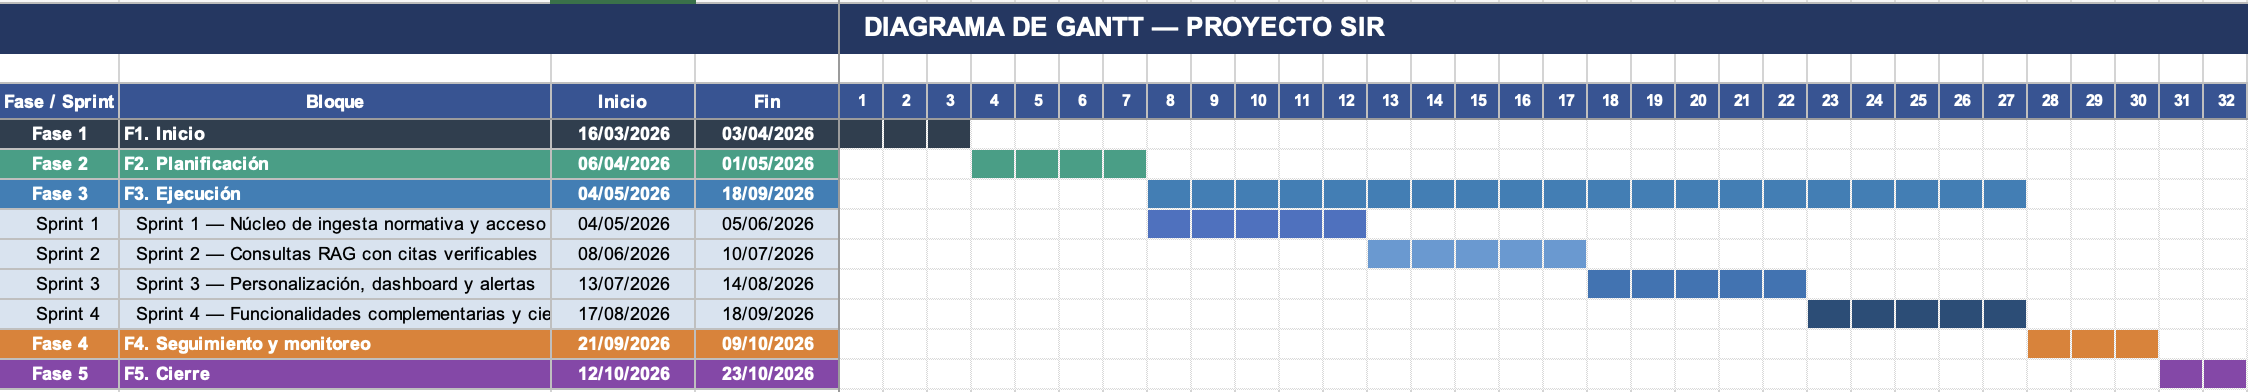
\includegraphics[width=10.4862in,height=2.18935in]{figuras/docx_image37.png}

\subsubsection{7.1.3 Plan de Gestión de
Costos}\label{plan-de-gestiuxf3n-de-costos}

\paragraph{7.1.3.1 Consideraciones de gestión de
costos}\label{consideraciones-de-gestiuxf3n-de-costos}

\phantomsection\label{_Toc231672306}{}Tabla 51\\
\emph{Consideraciones de gestión de costos}

\begin{longtable}[]{@{}
  >{\raggedright\arraybackslash}p{(\columnwidth - 2\tabcolsep) * \real{0.3774}}
  >{\raggedright\arraybackslash}p{(\columnwidth - 2\tabcolsep) * \real{0.6226}}@{}}
\toprule\noalign{}
\begin{minipage}[b]{\linewidth}\raggedright
Aspecto
\end{minipage} & \begin{minipage}[b]{\linewidth}\raggedright
Descripción
\end{minipage} \\
\midrule\noalign{}
\endhead
\bottomrule\noalign{}
\endlastfoot
Metodología de estimación & Estimación análoga (basada en proyectos
comparables) y paramétrica (precios públicos vigentes de AWS, OpenAI y
Pinecone). \\
Herramienta de estimación & Hoja de cálculo en Excel con tarifas
vigentes consultadas trimestralmente. \\
Unidades de tiempo & Mensual para servicios cloud, anual para dominio,
por millón de tokens para APIs de IA, por sprint para flujo de
costos. \\
Política de control & Monitoreo semanal del consumo de APIs en el
dashboard de OpenAI y AWS Cost Explorer. Alerta automática al alcanzar
el 80\% del presupuesto mensual. \\
\end{longtable}

\phantomsection\label{_Toc231672307}{}Tabla 52\\
\emph{Costos transversales del proyecto}

\begin{longtable}[]{@{}
  >{\raggedright\arraybackslash}p{(\columnwidth - 4\tabcolsep) * \real{0.6235}}
  >{\raggedright\arraybackslash}p{(\columnwidth - 4\tabcolsep) * \real{0.1640}}
  >{\raggedright\arraybackslash}p{(\columnwidth - 4\tabcolsep) * \real{0.2125}}@{}}
\toprule\noalign{}
\begin{minipage}[b]{\linewidth}\raggedright
Recurso
\end{minipage} & \begin{minipage}[b]{\linewidth}\raggedright
Cantidad
\end{minipage} & \begin{minipage}[b]{\linewidth}\raggedright
Costo total (S/)
\end{minipage} \\
\midrule\noalign{}
\endhead
\bottomrule\noalign{}
\endlastfoot
Servicios Cloud (AWS Compute + Storage) & 8 meses & 640.00 \\
Base vectorial Pinecone (free tier) & 8 meses & 0.00 \\
API OpenAI GPT-4 (consumo de tokens) & 8 meses & 960.00 \\
API OpenAI Embeddings & 8 meses & 225.00 \\
Dominio web .pe & 1 año & 180.00 \\
Servicio de email SendGrid (free tier) & 8 meses & 0.00 \\
Internet (trabajo remoto) & 8 meses & 800.00 \\
Electricidad & 8 meses & 400.00 \\
Materiales de oficina & global & 150.00 \\
Reserva de contingencia (10\%) & global & 335.50 \\
\textbf{TOTAL DESEMBOLSABLE} & --- & 3,690.50 \\
Recursos humanos valorizados & 1,240 hrs & 61,400.00 \\
\textbf{TOTAL PROYECTO VALORIZADO} & --- & 65,090.50 \\
\end{longtable}

\paragraph{7.1.3.2 Línea Base de Costos}\label{luxednea-base-de-costos}

\phantomsection\label{_Toc231672308}{}Tabla 53\\
\emph{Línea base de costos por mes}

\begin{longtable}[]{@{}
  >{\raggedright\arraybackslash}p{(\columnwidth - 10\tabcolsep) * \real{0.1212}}
  >{\raggedright\arraybackslash}p{(\columnwidth - 10\tabcolsep) * \real{0.1288}}
  >{\raggedright\arraybackslash}p{(\columnwidth - 10\tabcolsep) * \real{0.1624}}
  >{\raggedright\arraybackslash}p{(\columnwidth - 10\tabcolsep) * \real{0.1950}}
  >{\raggedright\arraybackslash}p{(\columnwidth - 10\tabcolsep) * \real{0.2275}}
  >{\raggedright\arraybackslash}p{(\columnwidth - 10\tabcolsep) * \real{0.1651}}@{}}
\toprule\noalign{}
\begin{minipage}[b]{\linewidth}\raggedright
Mes
\end{minipage} & \begin{minipage}[b]{\linewidth}\raggedright
Sprint
\end{minipage} & \begin{minipage}[b]{\linewidth}\raggedright
Cloud (S/)
\end{minipage} & \begin{minipage}[b]{\linewidth}\raggedright
APIs IA (S/)
\end{minipage} & \begin{minipage}[b]{\linewidth}\raggedright
Operativos (S/)
\end{minipage} & \begin{minipage}[b]{\linewidth}\raggedright
Total (S/)
\end{minipage} \\
\midrule\noalign{}
\endhead
\bottomrule\noalign{}
\endlastfoot
Mes 1 & 1 & 80 & 100 & 150 & 330 \\
Mes 2 & 1 & 80 & 100 & 150 & 330 \\
Mes 3 & 2 & 80 & 200 & 150 & 430 \\
Mes 4 & 2 & 80 & 200 & 150 & 430 \\
Mes 5 & 3 & 80 & 175 & 150 & 405 \\
Mes 6 & 3 & 80 & 175 & 150 & 405 \\
Mes 7 & 4 & 80 & 120 & 150 & 350 \\
Mes 8 & 4 & 80 & 115 & 150 & 345 \\
\textbf{TOTAL} & 8 meses & 640 & 1,185 & 1,200 & 3,025 \\
\end{longtable}

\subsubsection{7.1.4 Plan de Gestión de
Calidad}\label{plan-de-gestiuxf3n-de-calidad}

\paragraph{7.1.4.1 Consideraciones de gestión de
calidad}\label{consideraciones-de-gestiuxf3n-de-calidad}

\textbf{Política de calidad del proyecto:}

El proyecto adopta una política de calidad alineada al estándar ISO/IEC
25010 para calidad de producto de software, complementada con prácticas
de QA propias del marco ágil y los lineamientos del PMBOK®. Se priorizan
las características de Adecuación Funcional, Eficiencia de Desempeño,
Usabilidad, Fiabilidad, Seguridad y Mantenibilidad.

\textbf{Control de la Calidad (Producto):}

El control de calidad del Sistema de Inteligencia Regulatoria se ejecuta
sobre cada incremento de software al cierre del sprint. Las actividades
incluyen pruebas unitarias automatizadas (cobertura ≥ 80\%), pruebas de
integración de APIs, pruebas de carga al asistente RAG (50 usuarios
concurrentes con latencia p95 \textless{} 8 s), pruebas de precisión del
motor RAG (F1 ≥ 0.85 sobre 100 consultas etiquetadas) y pruebas de
usabilidad SUS al cierre del Sprint 4.

\textbf{Aseguramiento de la Calidad (Proceso de desarrollo del
producto):}

El aseguramiento de calidad se ejecuta de forma continua mediante (i)
revisiones de código por pares en cada Pull Request, (ii) cumplimiento
del Definition of Done en todas las HUs, (iii) auditorías internas
trimestrales del proceso ágil y (iv) actualización de la documentación
técnica con cada incremento. Las herramientas son GitHub para revisión
de código, GitHub Actions para CI/CD y SonarQube para métricas de
calidad estática.

\textbf{Calidad de la Gestión (Proyecto):}

La calidad del proyecto se monitorea con métricas PMBOK estándar: SPI
(Schedule Performance Index), CPI (Cost Performance Index), velocidad
del equipo, defect density y lead time. Cualquier desviación
significativa (SPI \textless{} 0.95 o CPI \textless{} 0.95) gatilla una
revisión con el asesor y un plan de acción documentado en la siguiente
retrospectiva.

\textbf{Responsables de Calidad (Proyecto):}

\phantomsection\label{_Toc231672309}{}Tabla 54\\
\emph{Responsables de calidad del proyecto}

\begin{longtable}[]{@{}
  >{\raggedright\arraybackslash}p{(\columnwidth - 4\tabcolsep) * \real{0.3333}}
  >{\raggedright\arraybackslash}p{(\columnwidth - 4\tabcolsep) * \real{0.3333}}
  >{\raggedright\arraybackslash}p{(\columnwidth - 4\tabcolsep) * \real{0.3333}}@{}}
\toprule\noalign{}
\begin{minipage}[b]{\linewidth}\raggedright
Responsable
\end{minipage} & \begin{minipage}[b]{\linewidth}\raggedright
Ámbito
\end{minipage} & \begin{minipage}[b]{\linewidth}\raggedright
Función
\end{minipage} \\
\midrule\noalign{}
\endhead
\bottomrule\noalign{}
\endlastfoot
Hervias Salas, Jadir & QA / Producto & Planificar y ejecutar pruebas,
validar criterios de aceptación, documentar defectos. \\
Hervias Salas, Jadir & Líder Técnico & Garantizar la calidad de la
arquitectura y del motor RAG. \\
Mogollón Buitrón, Khail & Jefe de Proyecto & Monitorear SPI, CPI,
velocidad y métricas de gestión. \\
Asesor PI-1 / PI-2 & Validación académica & Revisar entregables y
aprobar avances por sprint. \\
Boticas Farmaperu & Aceptación del producto & Validar criterios de
aceptación de las HUs y firmar la aceptación final. \\
\end{longtable}

\paragraph{7.1.4.2 Línea Base de
Calidad}\label{luxednea-base-de-calidad}

\phantomsection\label{_Toc231672310}{}Tabla 55\\
\emph{Línea base de calidad - factores, objetivos y métricas}

\begin{longtable}[]{@{}
  >{\raggedright\arraybackslash}p{(\columnwidth - 6\tabcolsep) * \real{0.2500}}
  >{\raggedright\arraybackslash}p{(\columnwidth - 6\tabcolsep) * \real{0.1931}}
  >{\raggedright\arraybackslash}p{(\columnwidth - 6\tabcolsep) * \real{0.3069}}
  >{\raggedright\arraybackslash}p{(\columnwidth - 6\tabcolsep) * \real{0.2500}}@{}}
\toprule\noalign{}
\begin{minipage}[b]{\linewidth}\raggedright
Factor de Calidad
\end{minipage} & \begin{minipage}[b]{\linewidth}\raggedright
Objetivo de Calidad
\end{minipage} & \begin{minipage}[b]{\linewidth}\raggedright
Métricas por usar (incluir fórmula)
\end{minipage} & \begin{minipage}[b]{\linewidth}\raggedright
Frecuencia y Momento de Reporte
\end{minipage} \\
\midrule\noalign{}
\endhead
\bottomrule\noalign{}
\endlastfoot
Rendimiento del proyecto (Costo) & CPI ≥ 0.95 & Indicador de costos: CPI
= Earned Value / Actual Cost & Mensualmente, la última semana del
mes. \\
Rendimiento del proyecto (Cronograma) & SPI ≥ 0.95 & Indicador de
cronograma: SPI = Earned Value / Planned Value & Mensualmente, la última
semana del mes. \\
Cumplimiento de Hitos & 95\% de cumplimiento & Hitos cumplidos / Hitos
planificados & Frecuencia mensual, acta de conformidad por
entregable. \\
Velocidad del equipo & ≥ 24 SP por sprint & Σ Story Points completados
por sprint & Por sprint, al cierre. \\
Cobertura de pruebas unitarias & ≥ 80\% & Líneas cubiertas / Total de
líneas & Continuo (CI), reporte por sprint. \\
Precisión del motor RAG & F1-Score ≥ 0.85 & F1 = 2 × (Precision ×
Recall) / (Precision + Recall) & Cierre de Sprint 2 y Sprint 4. \\
Cobertura de citaciones & ≥ 95\% & Respuestas con cita / Respuestas
totales × 100 & Cierre de Sprint 2 y Sprint 4. \\
Pruebas funcionales & Validación de criterios de aceptación al 100\% &
Pruebas funcionales = pruebas correctas / pruebas totales & Una vez
culminado el sprint. \\
Usabilidad & SUS ≥ 75 puntos & Promedio del cuestionario SUS de 10 ítems
& Cierre del Sprint 4. \\
Fiabilidad & Uptime ≥ 99\% & Tiempo activo / Tiempo total × 100 &
Mensual, durante PI-2. \\
Defect density & \textless{} 5 defectos / KLOC & Defectos detectados /
KLOC entregado & Por sprint. \\
Lead time & \textless{} 14 días por HU & Días promedio desde inicio
hasta entrega de HU & Por sprint. \\
\end{longtable}

\subsubsection{7.1.5 Plan de Gestión de
Riesgos}\label{plan-de-gestiuxf3n-de-riesgos}

\paragraph{7.1.5.1 Consideraciones de gestión de
riesgos}\label{consideraciones-de-gestiuxf3n-de-riesgos}

\phantomsection\label{_Toc231672311}{}Tabla 56\\
\emph{Matriz de probabilidad}

\begin{longtable}[]{@{}
  >{\raggedright\arraybackslash}p{(\columnwidth - 4\tabcolsep) * \real{0.3333}}
  >{\raggedright\arraybackslash}p{(\columnwidth - 4\tabcolsep) * \real{0.3333}}
  >{\raggedright\arraybackslash}p{(\columnwidth - 4\tabcolsep) * \real{0.3333}}@{}}
\toprule\noalign{}
\begin{minipage}[b]{\linewidth}\raggedright
Probabilidad
\end{minipage} & \begin{minipage}[b]{\linewidth}\raggedright
Valor
\end{minipage} & \begin{minipage}[b]{\linewidth}\raggedright
Descripción
\end{minipage} \\
\midrule\noalign{}
\endhead
\bottomrule\noalign{}
\endlastfoot
Muy probable & 5 & Probabilidad de que ocurra el evento ≥ 90\%. \\
Probable & 4 & Probabilidad de que ocurra el evento ≥ 70\% y \textless{}
90\%. \\
Moderado & 3 & Probabilidad de que ocurra el evento ≥ 50\% y \textless{}
70\%. \\
Improbable & 2 & Probabilidad de que ocurra el evento ≥ 25\% y
\textless{} 50\%. \\
Muy improbable & 1 & Probabilidad de que ocurra el evento \textless{}
25\%. \\
\end{longtable}

\phantomsection\label{_Toc231672312}{}Tabla 57\\
\emph{Matriz de impacto}

\begin{longtable}[]{@{}
  >{\raggedright\arraybackslash}p{(\columnwidth - 4\tabcolsep) * \real{0.2462}}
  >{\raggedright\arraybackslash}p{(\columnwidth - 4\tabcolsep) * \real{0.0984}}
  >{\raggedright\arraybackslash}p{(\columnwidth - 4\tabcolsep) * \real{0.6554}}@{}}
\toprule\noalign{}
\begin{minipage}[b]{\linewidth}\raggedright
Impacto
\end{minipage} & \begin{minipage}[b]{\linewidth}\raggedright
Valor
\end{minipage} & \begin{minipage}[b]{\linewidth}\raggedright
Descripción
\end{minipage} \\
\midrule\noalign{}
\endhead
\bottomrule\noalign{}
\endlastfoot
Muy Alto & 5 & El impacto influye directamente en el proyecto, pudiendo
ocasionar la cancelación del mismo. \\
Alto & 4 & El proyecto puede continuar pero con posibles pérdidas
económicas significativas. \\
Medio & 3 & El impacto puede demandar mayor esfuerzo y/o recursos. \\
Bajo & 2 & El impacto no tendría repercusiones en tiempos ni en
costos. \\
Muy Bajo & 1 & Si el impacto podemos aceptarlo. \\
\end{longtable}

\textbf{Matriz de Riesgo (Probabilidad × Impacto):}

Niveles de riesgo: Tolerable, Bajo, Medio, Alto, No tolerable (muy
alto). Se aplican estrategias diferenciadas por nivel.

\phantomsection\label{_Toc231672313}{}Tabla 58\\
\emph{Estrategia de matriz de riesgos}

\begin{longtable}[]{@{}
  >{\raggedright\arraybackslash}p{(\columnwidth - 10\tabcolsep) * \real{0.2575}}
  >{\raggedright\arraybackslash}p{(\columnwidth - 10\tabcolsep) * \real{0.1483}}
  >{\raggedright\arraybackslash}p{(\columnwidth - 10\tabcolsep) * \real{0.1512}}
  >{\raggedright\arraybackslash}p{(\columnwidth - 10\tabcolsep) * \real{0.1512}}
  >{\raggedright\arraybackslash}p{(\columnwidth - 10\tabcolsep) * \real{0.1459}}
  >{\raggedright\arraybackslash}p{(\columnwidth - 10\tabcolsep) * \real{0.1459}}@{}}
\toprule\noalign{}
\begin{minipage}[b]{\linewidth}\raggedright
Probabilidad
\end{minipage} & \begin{minipage}[b]{\linewidth}\raggedright
Imp 1
\end{minipage} & \begin{minipage}[b]{\linewidth}\raggedright
Imp 2
\end{minipage} & \begin{minipage}[b]{\linewidth}\raggedright
Imp 3
\end{minipage} & \begin{minipage}[b]{\linewidth}\raggedright
Imp 4
\end{minipage} & \begin{minipage}[b]{\linewidth}\raggedright
Imp 5
\end{minipage} \\
\midrule\noalign{}
\endhead
\bottomrule\noalign{}
\endlastfoot
P5 - Muy probable & 5 (Bajo) & 10 (Medio) & 15 (Alto) & 20 (No tol.) &
25 (No tol.) \\
P4 - Probable & 4 (Bajo) & 8 (Medio) & 12 (Alto) & 16 (No tol.) & 20 (No
tol.) \\
P3 - Moderado & 3 (Tolerable) & 6 (Medio) & 9 (Medio) & 12 (Alto) & 15
(Alto) \\
P2 - Improbable & 2 (Tolerable) & 4 (Bajo) & 6 (Medio) & 8 (Medio) & 10
(Medio) \\
P1 - Muy improbable & 1 (Tolerable) & 2 (Tolerable) & 3 (Tolerable) & 4
(Bajo) & 5 (Bajo) \\
\end{longtable}

\phantomsection\label{_Toc231672441}{}Figura\\
\emph{Matriz de Riesgos (Probabilidad × Impacto)}

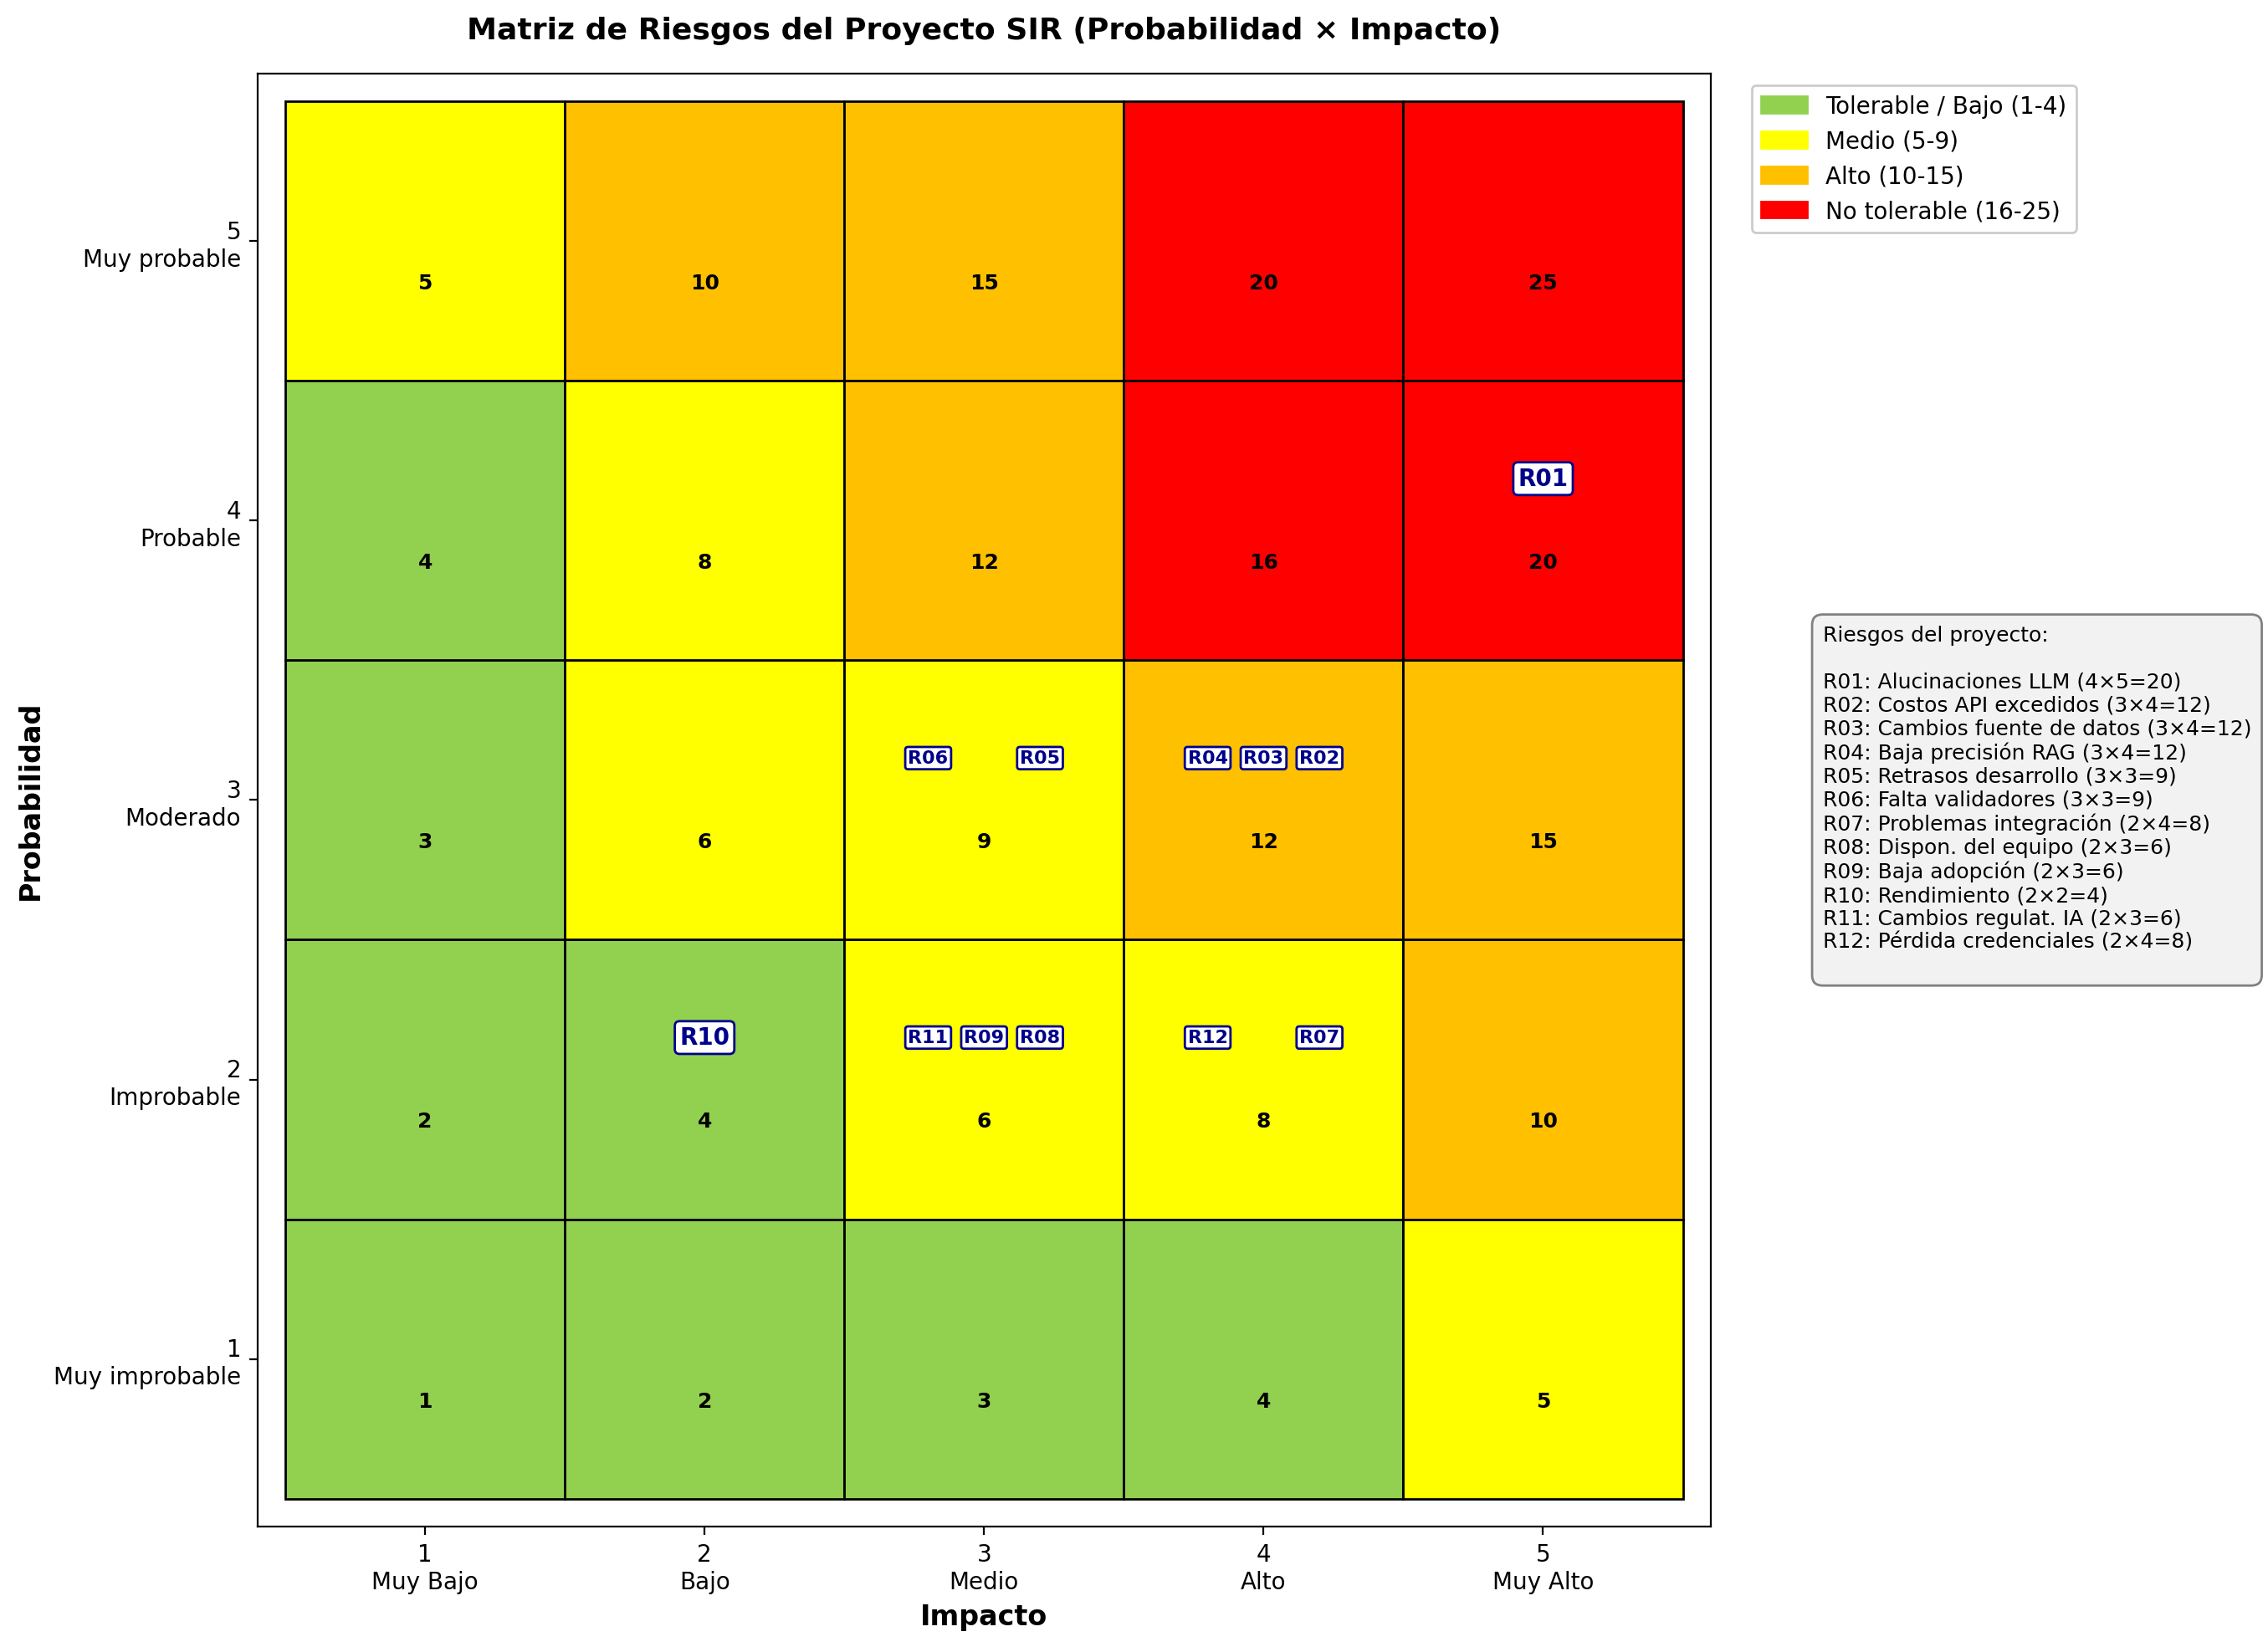
\includegraphics[width=6.5in,height=4.72083in]{figuras/docx_image38.png}

\paragraph{7.1.5.2 Línea Base del
Riesgo}\label{luxednea-base-del-riesgo}

\phantomsection\label{_Toc231672314}{}Tabla 59\\
\emph{Línea base de Riesgos}

\begin{longtable}[]{@{}
  >{\raggedright\arraybackslash}p{(\columnwidth - 16\tabcolsep) * \real{0.0419}}
  >{\raggedright\arraybackslash}p{(\columnwidth - 16\tabcolsep) * \real{0.0927}}
  >{\raggedright\arraybackslash}p{(\columnwidth - 16\tabcolsep) * \real{0.1751}}
  >{\raggedright\arraybackslash}p{(\columnwidth - 16\tabcolsep) * \real{0.0532}}
  >{\raggedright\arraybackslash}p{(\columnwidth - 16\tabcolsep) * \real{0.0726}}
  >{\raggedright\arraybackslash}p{(\columnwidth - 16\tabcolsep) * \real{0.0907}}
  >{\raggedright\arraybackslash}p{(\columnwidth - 16\tabcolsep) * \real{0.1843}}
  >{\raggedright\arraybackslash}p{(\columnwidth - 16\tabcolsep) * \real{0.0861}}
  >{\raggedright\arraybackslash}p{(\columnwidth - 16\tabcolsep) * \real{0.2034}}@{}}
\toprule\noalign{}
\begin{minipage}[b]{\linewidth}\raggedright
N°
\end{minipage} & \begin{minipage}[b]{\linewidth}\raggedright
Fecha de registro
\end{minipage} & \begin{minipage}[b]{\linewidth}\raggedright
Riesgo
\end{minipage} & \begin{minipage}[b]{\linewidth}\raggedright
Prob.
\end{minipage} & \begin{minipage}[b]{\linewidth}\raggedright
Impacto
\end{minipage} & \begin{minipage}[b]{\linewidth}\raggedright
Exposición
\end{minipage} & \begin{minipage}[b]{\linewidth}\raggedright
Trigger
\end{minipage} & \begin{minipage}[b]{\linewidth}\raggedright
Estrategia
\end{minipage} & \begin{minipage}[b]{\linewidth}\raggedright
Respuesta
\end{minipage} \\
\midrule\noalign{}
\endhead
\bottomrule\noalign{}
\endlastfoot
R01 & 06/05/2026 & Alucinaciones del LLM: el modelo genera información
legal incorrecta o sin sustento en el corpus. & 4 & 5 & 20 & Tasa de
respuestas incorrectas en pruebas piloto \textgreater{} 5\%. & Mitigar &
RAG estricto que solo responde con contexto recuperado; validación de
citas obligatorias; disclaimer legal. \\
R02 & 06/05/2026 & Costos de API OpenAI excedidos. & 3 & 4 & 12 & Gasto
mensual \textgreater{} 80\% del presupuesto antes del día 20. & Mitigar
& Límites de gasto diario/mensual + caché de respuestas + modelos
económicos en desarrollo. \\
R03 & 06/05/2026 & Cambios en la fuente de datos: El Peruano o DIGEMID
modifican su web o bloquean el scraper. & 3 & 4 & 12 & El scraper falla
por \textgreater{} 3 días consecutivos. & Mitigar & Conector modular +
monitoreo de cambios estructurales + scraping manual de respaldo. \\
R04 & 06/05/2026 & Baja precisión del motor RAG. & 3 & 4 & 12 & F1-Score
\textless{} 0.80 al cierre de Sprint 2. & Mitigar & Iteración de prompts
+ mejor chunking + modelos alternativos + ampliar dataset de pruebas. \\
R05 & 06/05/2026 & Retrasos en el desarrollo. & 3 & 3 & 9 & Velocidad
\textless{} 18 SP en dos sprints consecutivos. & Mitigar & Buffer 15\%
en estimaciones + priorizar Must Have + reducir Could Have si es
necesario. \\
R06 & 06/05/2026 & Falta de validadores externos para SUS y experimento.
& 3 & 3 & 9 & Al inicio de Sprint 3 no hay 5 PYMEs comprometidas. &
Mitigar & Contactar PYMEs farmacéuticas desde Sprint 1 + acceso gratuito
por feedback. \\
R07 & 06/05/2026 & Problemas de integración entre frontend, backend e
IA. & 2 & 4 & 8 & PRs con \textgreater{} 30\% de fallos en pruebas de
integración. & Mitigar & CI/CD desde Sprint 1 + APIs documentadas con
OpenAPI + pruebas de integración automatizadas. \\
R08 & 06/05/2026 & Disponibilidad del equipo afectada. & 2 & 3 & 6 & Un
miembro reporta indisponibilidad \textgreater{} 1 semana. & Aceptar /
Mitigar & Documentación continua + handoff + replantear alcance. \\
R09 & 06/05/2026 & Baja adopción por desconfianza en IA. & 2 & 3 & 6 &
SUS \textless{} 65 puntos en pruebas piloto. & Mitigar & Disclaimers +
fuentes verificables + validación con abogado en pruebas + capacitación
corta a usuarios. \\
R10 & 06/05/2026 & Problemas de rendimiento. & 2 & 2 & 4 & Latencia p95
\textgreater{} 12 s en pruebas de carga. & Aceptar & MVP con pocos
usuarios; monitorear y escalar post-lanzamiento. \\
R11 & 06/05/2026 & Cambios regulatorios sobre IA en el Perú (Ley N.º
31814). & 2 & 3 & 6 & Publicación de reglamento que afecte el alcance. &
Mitigar & Monitoreo regulatorio mensual + diseño flexible que permita
ajustar el componente generativo y los disclaimers. \\
R12 & 06/05/2026 & Pérdida de credenciales por mal manejo del
repositorio. & 2 & 4 & 8 & Commit accidental con credenciales en GitHub
público. & Evitar & .gitignore + git-secrets + variables en secretos del
CI/CD + backups semanales. \\
\end{longtable}

\subsubsection{7.1.6 Plan de Gestión de
Comunicaciones}\label{plan-de-gestiuxf3n-de-comunicaciones}

\paragraph{7.1.6.1 Consideraciones de gestión de
comunicaciones}\label{consideraciones-de-gestiuxf3n-de-comunicaciones}

Para todas las reuniones que se lleven a cabo durante el desarrollo del
proyecto se seguirán las siguientes pautas:

\begin{itemize}
\item
  Las reuniones del equipo y con el asesor se realizan vía
  videoconferencia (Microsoft Teams, Google Meet o Zoom) y
  presencialmente en la UPC cuando sea factible.
\item
  Las reuniones con Boticas Farmaperu se realizan presencialmente en su
  local o por videoconferencia, según disponibilidad.
\item
  Cualquier comunicación formal con el asesor se registra por correo
  electrónico de la UPC.
\item
  Las reuniones con el asesor de tesis se programan previa coordinación,
  con frecuencia quincenal.
\item
  Si algún asistente no puede ingresar a una reunión, lo avisa por
  correo con al menos 12 horas de anticipación.
\item
  Si la reunión no se realiza, se reprograma previa coordinación.
\item
  En cada reunión se tratan los temas de interés y los pendientes de
  reuniones anteriores.
\item
  Al finalizar cada reunión se elabora un acta con los puntos tratados y
  los acuerdos pactados.
\item
  Las actas son firmadas por los asistentes y el asesor.
\end{itemize}

\paragraph{7.1.6.2 Línea Base de
Comunicaciones}\label{luxednea-base-de-comunicaciones}

\phantomsection\label{_Toc231672315}{}Tabla 60\\
\emph{Matriz de Riesgos (Probabilidad × Impacto)}

\begin{longtable}[]{@{}
  >{\raggedright\arraybackslash}p{(\columnwidth - 12\tabcolsep) * \real{0.1600}}
  >{\raggedright\arraybackslash}p{(\columnwidth - 12\tabcolsep) * \real{0.1346}}
  >{\raggedright\arraybackslash}p{(\columnwidth - 12\tabcolsep) * \real{0.1022}}
  >{\raggedright\arraybackslash}p{(\columnwidth - 12\tabcolsep) * \real{0.1224}}
  >{\raggedright\arraybackslash}p{(\columnwidth - 12\tabcolsep) * \real{0.1346}}
  >{\raggedright\arraybackslash}p{(\columnwidth - 12\tabcolsep) * \real{0.1834}}
  >{\raggedright\arraybackslash}p{(\columnwidth - 12\tabcolsep) * \real{0.1627}}@{}}
\toprule\noalign{}
\begin{minipage}[b]{\linewidth}\raggedright
Contenido
\end{minipage} & \begin{minipage}[b]{\linewidth}\raggedright
Formato
\end{minipage} & \begin{minipage}[b]{\linewidth}\raggedright
Nivel de detalle
\end{minipage} & \begin{minipage}[b]{\linewidth}\raggedright
Responsable de comunicar
\end{minipage} & \begin{minipage}[b]{\linewidth}\raggedright
Grupo receptor
\end{minipage} & \begin{minipage}[b]{\linewidth}\raggedright
Metodología/Tecnología
\end{minipage} & \begin{minipage}[b]{\linewidth}\raggedright
Frecuencia
\end{minipage} \\
\midrule\noalign{}
\endhead
\bottomrule\noalign{}
\endlastfoot
Definición del proyecto & Project Charter & Alto & Jefe de Proyecto &
Asesor PI-1, jurado, equipo & PDF en repositorio Git & Una sola vez (Sem
1) \\
Planificación detallada del proyecto & Planes PMBOK & Muy Alto & Jefe de
Proyecto & Asesor, equipo & Word + PDF en SharePoint & Una sola vez (Sem
2-3) \\
Avances quincenales & Reporte de avance & Medio & Scrum Master & Asesor,
equipo & Reunión virtual + acta firmada & Quincenal \\
Sprint Backlog y Burndown & Tablero Trello + gráfico & Medio & Scrum
Master & Equipo & Trello + Excel & Diario / cierre del sprint \\
Daily Meeting & Reunión virtual breve & Bajo & Cada miembro & Equipo &
Microsoft Teams (15 min) & 2 veces por semana \\
Sprint Review & Demo + acta & Alto & Scrum Master & Asesor, PYME piloto,
equipo & Reunión virtual con demo & Cierre de cada sprint \\
Sprint Retrospective & Acta interna & Medio & Scrum Master & Equipo &
Microsoft Teams + Miro & Cierre de cada sprint \\
Reportes mensuales de costos & Excel + dashboard OpenAI & Medio & Jefe
de Proyecto & Equipo & Excel + capturas & Mensual \\
Reportes de calidad por sprint & Reporte QA & Alto & Analista QA &
Asesor, equipo & Documento PDF & Cierre de cada sprint \\
Comunicación con la PYME piloto & Correo + reunión & Medio & Product
Owner & Representante PYME & Email + WhatsApp + reunión & Quincenal \\
Cierre del proyecto y entrega final & Memoria + sustentación & Muy Alto
& Jefe de Proyecto & Jurado, asesor, PYME piloto & Documento Word +
sustentación oral & Una sola vez (Sem 32) \\
\end{longtable}

\subsubsection{7.1.7 Plan de Gestión de
Interesados}\label{plan-de-gestiuxf3n-de-interesados}

\paragraph{7.1.7.1 Consideraciones de gestión de
interesados}\label{consideraciones-de-gestiuxf3n-de-interesados}

La gestión de interesados se ejecuta en cuatro fases: identificación,
análisis (poder/interés), planificación de compromiso y monitoreo. Se
prioriza la comunicación con los interesados de alto poder y alto
interés (asesor, Boticas Farmaperu), manteniendo informados a los de
bajo poder pero alto interés (otros stakeholders) y satisfechos a los de
alto poder y bajo interés (jurado).

\paragraph{7.1.7.2 Línea Base de
Interesados}\label{luxednea-base-de-interesados}

\phantomsection\label{_Toc231672316}{}Tabla 61\\
\emph{Registro de interesados del proyecto}

\begin{longtable}[]{@{}
  >{\raggedright\arraybackslash}p{(\columnwidth - 10\tabcolsep) * \real{0.0577}}
  >{\raggedright\arraybackslash}p{(\columnwidth - 10\tabcolsep) * \real{0.2981}}
  >{\raggedright\arraybackslash}p{(\columnwidth - 10\tabcolsep) * \real{0.1154}}
  >{\raggedright\arraybackslash}p{(\columnwidth - 10\tabcolsep) * \real{0.0769}}
  >{\raggedright\arraybackslash}p{(\columnwidth - 10\tabcolsep) * \real{0.0577}}
  >{\raggedright\arraybackslash}p{(\columnwidth - 10\tabcolsep) * \real{0.3942}}@{}}
\toprule\noalign{}
\begin{minipage}[b]{\linewidth}\raggedright
ID
\end{minipage} & \begin{minipage}[b]{\linewidth}\raggedright
Interesado
\end{minipage} & \begin{minipage}[b]{\linewidth}\raggedright
Categoría
\end{minipage} & \begin{minipage}[b]{\linewidth}\raggedright
Interés
\end{minipage} & \begin{minipage}[b]{\linewidth}\raggedright
Poder
\end{minipage} & \begin{minipage}[b]{\linewidth}\raggedright
Estrategia
\end{minipage} \\
\midrule\noalign{}
\endhead
\bottomrule\noalign{}
\endlastfoot
I1 & Asesor PI-1 (Zacarías Ramos, Juan) & Académico & Alto & Alto &
Gestionar de cerca: reuniones quincenales, validar entregables. \\
I2 & Asesor PI-2 (por confirmar) & Académico & Alto & Alto & Gestionar
de cerca: continuar metodología establecida en PI-1. \\
I3 & Boticas Farmaperu - Sponsor & Cliente & Alto & Alto & Gestionar de
cerca: reuniones quincenales, demos, validar HUs. \\
I4 & Boticas Farmaperu - Usuario líder & Usuario final & Alto & Medio &
Mantener informado y comprometido: validar HUs, aplicar SUS y
experimento de tiempo. \\
I5 & Jurado de tesis & Académico & Bajo & Alto & Mantener satisfecho:
presentaciones formales en PI-1 y PI-2, documento final con calidad
APA. \\
I6 & Equipo del proyecto (Khail, Jadir) & Interno & Muy Alto & Alto &
Gestionar de cerca: comunicación diaria, alineación de objetivos. \\
I7 & Otras PYMEs farmacéuticas (encuesta diagnóstica) & Externo & Bajo &
Bajo & Monitorear: agradecimiento por participación. \\
I8 & Proveedores SaaS (OpenAI, Pinecone, SendGrid) & Proveedor & Bajo &
Medio & Mantener informado: cumplir términos de servicio. \\
I9 & DIGEMID y Editora Perú (fuentes de datos) & Externo & Bajo & Alto &
Mantener satisfecho: respetar términos de uso, citar correctamente. \\
I10 & Comunidad académica (publicación posterior) & Externo & Bajo &
Bajo & Monitorear: preparar publicación al cierre del proyecto. \\
\end{longtable}

\phantomsection\label{_Toc231672317}{}Tabla 62\\
\emph{Matriz de poder e interés}

\begin{longtable}[]{@{}
  >{\raggedright\arraybackslash}p{(\columnwidth - 6\tabcolsep) * \real{0.2500}}
  >{\raggedright\arraybackslash}p{(\columnwidth - 6\tabcolsep) * \real{0.0883}}
  >{\raggedright\arraybackslash}p{(\columnwidth - 6\tabcolsep) * \real{0.1029}}
  >{\raggedright\arraybackslash}p{(\columnwidth - 6\tabcolsep) * \real{0.5588}}@{}}
\toprule\noalign{}
\begin{minipage}[b]{\linewidth}\raggedright
Cuadrante
\end{minipage} & \begin{minipage}[b]{\linewidth}\raggedright
Poder
\end{minipage} & \begin{minipage}[b]{\linewidth}\raggedright
Interés
\end{minipage} & \begin{minipage}[b]{\linewidth}\raggedright
Interesados
\end{minipage} \\
\midrule\noalign{}
\endhead
\bottomrule\noalign{}
\endlastfoot
Gestionar de cerca & Alto & Alto & Asesor PI-1 (I1), Asesor PI-2 (I2),
Sponsor PYME (I3), Equipo (I6) \\
Mantener satisfecho & Alto & Bajo & Jurado de tesis (I5),
DIGEMID/Editora Perú (I9) \\
Mantener informado & Bajo & Alto & Usuario líder PYME (I4) \\
Monitorear & Bajo & Bajo & Otras PYMEs (I7), Proveedores SaaS (I8),
Comunidad académica (I10) \\
\end{longtable}

\subsection{7.2 Ejecución y monitoreo
PI-1}\label{ejecuciuxf3n-y-monitoreo-pi-1}

En esta sección se reporta la ejecución y el monitoreo del proyecto
durante el primer ciclo académico (PI-1), centrado en el Sprint 1. El
seguimiento del estado global del proyecto se consolida en el panel de
ejecución y monitoreo (Figura --- Panel de ejecución y monitoreo del
estado del proyecto de investigación 1). A continuación, se detalla la
ejecución por cada área de conocimiento.

\textbf{Plan de Gestión del Alcance}

Siguiendo el progreso del plan de gestión del alcance de esta primera
fase de ejecución y monitoreo de PI-1, se completó la implementación de
los paquetes de Inicio, Planificación y Análisis y Diseño, alcanzando el
desarrollo hasta el Sprint 1, conforme a la línea base del EDT.

Avances en el desarrollo. Se completaron las siguientes historias de
usuario en el Sprint 1:

HU01: Registro de usuario y empresa

HU02: Autenticación y roles

HU04: Ingesta automática de normas

HU05: Limpieza y normalización textual

HU06: Vectorización de documentos

Estos avances se alinean con la definición del alcance del proyecto:
construir el acceso seguro y el pipeline de ingesta normativa que
habilitan la arquitectura RAG del SIR.

Revisión de avances.

Se evaluó el progreso alcanzado en el Sprint 1, incluyendo la revisión
retrospectiva del sprint.

Se identificaron las tareas cumplidas, las que quedan en curso y las
pendientes para los objetivos del proyecto.

Evaluación preliminar de resultados. El incremento del Sprint 1 es de
carácter habilitador: deja operativa la base de datos, la seguridad, la
ingesta y el corpus vectorizado. Los indicadores de impacto (precisión
del motor RAG, cobertura de citaciones y satisfacción del usuario) se
medirán en los sprints de validación.

\textbf{Plan de Gestión del Cronograma}

Para la gestión del cronograma de la primera fase de ejecución y
monitoreo se siguió el avance del Sprint 1 mediante el Sprint Burndown
Chart (Figura --- Burndown Chart del Sprint 1), que compara la línea
ideal de 24 story points con la línea real a lo largo de las cinco
semanas (25 días hábiles) del sprint. Para monitorear el progreso de las
tareas se elaboró la siguiente tabla, que compara lo planeado con lo
ejecutado.

Tabla --- Control y monitoreo del desarrollo del Sprint 1

\begin{longtable}[]{@{}
  >{\raggedright\arraybackslash}p{(\columnwidth - 12\tabcolsep) * \real{0.1429}}
  >{\raggedright\arraybackslash}p{(\columnwidth - 12\tabcolsep) * \real{0.1429}}
  >{\raggedright\arraybackslash}p{(\columnwidth - 12\tabcolsep) * \real{0.1429}}
  >{\raggedright\arraybackslash}p{(\columnwidth - 12\tabcolsep) * \real{0.1429}}
  >{\raggedright\arraybackslash}p{(\columnwidth - 12\tabcolsep) * \real{0.1429}}
  >{\raggedright\arraybackslash}p{(\columnwidth - 12\tabcolsep) * \real{0.1429}}
  >{\raggedright\arraybackslash}p{(\columnwidth - 12\tabcolsep) * \real{0.1429}}@{}}
\toprule\noalign{}
\begin{minipage}[b]{\linewidth}\raggedright
\textbf{Tareas}
\end{minipage} & \begin{minipage}[b]{\linewidth}\raggedright
\textbf{HU01}
\end{minipage} & \begin{minipage}[b]{\linewidth}\raggedright
\textbf{HU02}
\end{minipage} & \begin{minipage}[b]{\linewidth}\raggedright
\textbf{HU04}
\end{minipage} & \begin{minipage}[b]{\linewidth}\raggedright
\textbf{HU05}
\end{minipage} & \begin{minipage}[b]{\linewidth}\raggedright
\textbf{HU06}
\end{minipage} & \begin{minipage}[b]{\linewidth}\raggedright
\textbf{Total}
\end{minipage} \\
\midrule\noalign{}
\endhead
\bottomrule\noalign{}
\endlastfoot
\textbf{Planeado} & 3 días & 3 días & 8 días & 5 días & 6 días & 25
días \\
\textbf{Ejecutado} & 3 días & 3 días & 10 días & 5 días & 4 días & 25
días \\
\end{longtable}

\emph{\textbf{Resultados.}} El Sprint 1 se cerró dentro del plazo
previsto (05/06/2026). A continuación se describen los eventos:

La ingesta automática de normas (HU04) demandó dos días adicionales por
la variabilidad de las fuentes oficiales (PDF/HTML) y los rangos de
fechas sin resultados.

El retraso se absorbió con el buffer del sprint y la reasignación de
esfuerzo, sin afectar el cierre.

Se mantuvo la velocidad planificada de 24 story points y se cumplieron
todas las historias comprometidas.

\textbf{Plan de Gestión de los Costos}

Durante el Sprint 1 no se generaron sobrecostos. La ejecución se mantuvo
dentro de la línea base: se utilizaron los planes free-tier de la
infraestructura cloud (con un costo estimado de US\$ 5--7 mensuales) y
no se consumieron créditos de OpenAI, ya que se decidió mantener la IA
generativa configurable pero no obligatoria en este incremento,
reservándola para los sprints de generación y evaluación. El
almacenamiento vectorial se resolvió con PostgreSQL + pgvector, evitando
costos adicionales de bases de datos especializadas.

\textbf{Plan de Gestión de la Calidad}

La ejecución del plan de calidad cumplió con los estándares establecidos
desde el inicio del proyecto hasta el cierre del Sprint 1. Se mantuvo un
seguimiento constante de los entregables, lo que permitió detectar y
resolver desviaciones de manera oportuna, asegurando la calidad del
trabajo realizado. El control de la calidad del producto se documenta en
la Sección 5.1 mediante las métricas ISO/IEC 25010.

Resultados.

Cada historia se consideró cerrada tras cumplir la Definición de
Terminado (DoD) y obtener la aprobación del Product Owner en el Sprint
Review.

En las pruebas de calidad se ejecutaron con éxito los cinco casos de
prueba (CP001 a CP005), sin defectos críticos abiertos.

El incremento se evaluó con las características ISO/IEC 25010:
adecuación funcional, eficiencia, usabilidad, fiabilidad, seguridad y
mantenibilidad (Sección 5.1).

\textbf{Plan de Gestión de los Riesgos}

Durante la ejecución del Sprint 1 se gestionaron los riesgos
materializados, principalmente la variabilidad de las fuentes normativas
y los costos potenciales de IA.

Tabla --- Ejecución del proyecto: riesgos del Sprint 1

\begin{longtable}[]{@{}
  >{\raggedright\arraybackslash}p{(\columnwidth - 2\tabcolsep) * \real{0.5000}}
  >{\raggedright\arraybackslash}p{(\columnwidth - 2\tabcolsep) * \real{0.5000}}@{}}
\toprule\noalign{}
\begin{minipage}[b]{\linewidth}\raggedright
\textbf{Riesgo}
\end{minipage} & \begin{minipage}[b]{\linewidth}\raggedright
\textbf{Plan de mitigación}
\end{minipage} \\
\midrule\noalign{}
\endhead
\bottomrule\noalign{}
\endlastfoot
Variabilidad de las fuentes normativas (PDF/HTML) y rangos de fechas sin
documentos. & Conector modular con logs detallados y trazabilidad (URL,
checksum, items\_discovered); distinción entre ausencia real y error de
extracción. \\
Costos potenciales de IA por uso de OpenAI. & Reservar OpenAI solo para
tareas de generación/evaluación; resolver operaciones determinísticas
sin API. \\
Riesgo de alucinaciones del modelo en respuestas (R01). & Diseño RAG
estricto restringido a la evidencia, con trazabilidad de cada fragmento
de cara al Sprint 2. \\
\end{longtable}

\emph{\textbf{Resultados:}}

Los problemas de ingesta se controlaron con logs y trazabilidad, sin
detener el resto del sistema.

El monitoreo en las dailies y la revisión quincenal de la matriz de
riesgos mantuvieron el control del cronograma.

Las decisiones técnicas estuvieron alineadas con los objetivos y el
presupuesto del proyecto.

\textbf{Plan de Gestión de las Comunicaciones}

Para mantener un seguimiento efectivo de la comunicación durante la
ejecución se aplicó lo establecido en el plan de gestión de las
comunicaciones. Se cumplieron las siguientes pautas:

Realizar las ceremonias Scrum (Planning, Daily, Review y Retrospective)
y anexar sus actas.

Mantener las asesorías quincenales con el asesor de PI-1 y registrar sus
actas.

Notificar cualquier modificación en la documentación y reportar
incidentes que surjan.

Mantener comunicación constante con el Product Owner y actualizar el
Site del proyecto en SharePoint.

\textbf{Plan de Gestión de los Interesados}

Para medir el grado de satisfacción del Product Owner se realizaron
reuniones a lo largo del Sprint 1. El Product Owner manifestó su
conformidad con el avance del incremento y validó la decisión de no
depender obligatoriamente de OpenAI en esta etapa. Su feedback se
registró en el acta del Sprint Review y se incorporó a los compromisos
del Sprint 2. Las actas de reuniones están disponibles en la sección de
anexos.

\subsection{7.4 Lecciones Aprendidas}\label{lecciones-aprendidas}

Las lecciones aprendidas se documentan al cierre del proyecto siguiendo
el formato What-So What-Now What. Se clasifican por área de conocimiento
y por categoría (procesos, tecnología, equipo).

\phantomsection\label{_Toc231672318}{}Tabla 63\\
\emph{Lecciones aprendidas del proyecto}

\begin{longtable}[]{@{}
  >{\raggedright\arraybackslash}p{(\columnwidth - 4\tabcolsep) * \real{0.1827}}
  >{\raggedright\arraybackslash}p{(\columnwidth - 4\tabcolsep) * \real{0.4711}}
  >{\raggedright\arraybackslash}p{(\columnwidth - 4\tabcolsep) * \real{0.3461}}@{}}
\toprule\noalign{}
\begin{minipage}[b]{\linewidth}\raggedright
Categoría
\end{minipage} & \begin{minipage}[b]{\linewidth}\raggedright
Lección aprendida
\end{minipage} & \begin{minipage}[b]{\linewidth}\raggedright
Acción recomendada para futuros proyectos
\end{minipage} \\
\midrule\noalign{}
\endhead
\bottomrule\noalign{}
\endlastfoot
Procesos -- Alcance & La adopción del régimen MoSCoW combinada con la
priorización por valor de negocio resultó útil para gestionar el alcance
del SIR, pero requirió varios refinamientos del Product Backlog ante
cambios en la operación de Boticas Farmaperu. La separación entre HUs
Must Have y Should Have evitó el sobre-alcance del PI-1. & Reservar al
menos una sesión de refinamiento por sprint con participación del
usuario líder de la PYME, y mantener un registro vivo de cambios de
alcance con su justificación de negocio. \\
Procesos -- Cronograma & El monitoreo semanal del SPI y los daily
meetings de dos sesiones por semana fueron suficientes para detectar
desvíos a tiempo. Las ceremonias presenciales con el asesor cada 15 días
ayudaron a recalibrar el sprint en curso. & Mantener buffers de 15\% en
estimaciones para HUs con dependencias externas (ingesta de El Peruano,
APIs de OpenAI), y usar burndown chart compartido en Trello para
anticipar bloqueos. \\
Procesos -- Calidad & El cumplimiento del Definition of Done por sprint
y las pruebas de precisión del motor RAG en cada incremento permitieron
mantener el F1-Score por encima del umbral durante el desarrollo. La
validación con el Product Owner antes de cerrar el sprint fue
determinante para evitar reprocesos. & Formalizar la prueba de precisión
RAG con un dataset etiquetado por al menos un experto legal externo
desde el Sprint 1, y automatizar la regresión de calidad en CI/CD. \\
Procesos -- Riesgo & El riesgo R01 (alucinaciones del LLM) se mantuvo
controlado gracias al RAG estricto y la validación obligatoria de citas.
El riesgo R02 (costos de API) fue el más sensible y requirió implementar
caché y modelos económicos en desarrollo desde el Sprint 2. & Asignar un
responsable rotativo de monitoreo de riesgos por sprint y definir
umbrales automáticos de alerta sobre costos de OpenAI, latencia y
precisión que disparen revisión inmediata. \\
Tecnología -- RAG / IA Generativa & La arquitectura RAG con GPT-4 +
Pinecone demostró ser apropiada para el dominio normativo peruano, pero
la calidad del chunking y de la curación del corpus normativo resultaron
tanto o más determinantes que el modelo generativo. La cobertura de
citaciones se logró únicamente con un retriever que devuelve metadatos
completos (norma, artículo, entidad, fecha). & Invertir tiempo
significativo en curar el corpus normativo (limpieza, segmentación por
estructura legal y enriquecimiento de metadatos) antes de optimizar
prompts. Probar al menos dos estrategias de chunking y comparar
F1-Score. \\
Tecnología -- Arquitectura & El modelo C4 facilitó la comunicación
arquitectónica con el asesor y permitió que las decisiones de diseño
quedaran trazables. La separación entre frontend (React + TS), backend
(FastAPI) y motor RAG (LangChain) habilitó despliegues independientes y
reduce el riesgo en producción. & Mantener los diagramas C4 versionados
en el repositorio (draw.io) y actualizarlos al cierre de cada sprint.
Documentar cada decisión arquitectónica con un ADR (Architecture
Decision Record). \\
Equipo -- Comunicación & Las dailies de dos sesiones por semana, las
asesorías quincenales y la matriz de comunicaciones formal ayudaron a
sostener el alineamiento entre los dos integrantes y con el sponsor de
Boticas Farmaperu. La comunicación por WhatsApp y correo permitió una
coordinación ágil con el usuario líder de la PYME. & Mantener actas
firmadas de toda reunión formal y consolidar un repositorio único
(SharePoint o Drive) con todos los entregables ordenados por sprint para
facilitar la trazabilidad ante revisión académica. \\
Equipo -- Capacitación & El autoaprendizaje en RAG, embeddings, vector
databases y LangChain fue intensivo y demandó tiempo no planificado en
los primeros sprints. Cursos de Coursera y DeepLearning.AI fueron
recursos efectivos. El conocimiento previo de Python y React redujo la
curva de aprendizaje técnico. & Dedicar al menos dos semanas iniciales
del proyecto a capacitación dirigida sobre tecnologías nuevas (RAG,
vectorización, prompt engineering) antes de iniciar la construcción, y
registrar el conocimiento en una wiki interna del equipo para futuros
proyectos. \\
\end{longtable}

\section{Glosario de Términos}\label{glosario-de-tuxe9rminos}

\begin{longtable}[]{@{}
  >{\raggedright\arraybackslash}p{(\columnwidth - 2\tabcolsep) * \real{0.2272}}
  >{\raggedright\arraybackslash}p{(\columnwidth - 2\tabcolsep) * \real{0.7728}}@{}}
\toprule\noalign{}
\begin{minipage}[b]{\linewidth}\raggedright
Término
\end{minipage} & \begin{minipage}[b]{\linewidth}\raggedright
Definición
\end{minipage} \\
\midrule\noalign{}
\endhead
\bottomrule\noalign{}
\endlastfoot
Chunking & Técnica de segmentación de un documento en fragmentos
coherentes para su procesamiento por modelos de lenguaje. \\
Embeddings & Representaciones vectoriales densas de palabras, frases o
documentos en un espacio semántico. \\
LLM & Modelo de Lenguaje de Gran Escala (Large Language Model) entrenado
para tareas de comprensión y generación de texto. \\
MoSCoW & Técnica de priorización: Must have, Should have, Could have,
Won\textquotesingle t have. \\
Planning Poker & Técnica de estimación colaborativa basada en escala
Fibonacci. \\
Product Backlog & Lista priorizada de Historias de Usuario y requisitos
del producto. \\
RAG & Retrieval-Augmented Generation: arquitectura que combina
recuperación de información con generación de texto. \\
RegTech & Tecnologías aplicadas al cumplimiento regulatorio. \\
Sprint & Iteración de desarrollo de duración fija en Scrum. \\
SUS & System Usability Scale, cuestionario estandarizado de
usabilidad. \\
User Story Mapping & Técnica de visualización de historias por proceso
para identificar MVPs y orden de entrega. \\
\end{longtable}

\section{Siglario}\label{siglario}

\begin{longtable}[]{@{}
  >{\raggedright\arraybackslash}p{(\columnwidth - 2\tabcolsep) * \real{0.1699}}
  >{\raggedright\arraybackslash}p{(\columnwidth - 2\tabcolsep) * \real{0.8301}}@{}}
\toprule\noalign{}
\begin{minipage}[b]{\linewidth}\raggedright
Sigla
\end{minipage} & \begin{minipage}[b]{\linewidth}\raggedright
Significado
\end{minipage} \\
\midrule\noalign{}
\endhead
\bottomrule\noalign{}
\endlastfoot
AWS & Amazon Web Services \\
CAGR & Compound Annual Growth Rate \\
CIIU & Clasificación Industrial Internacional Uniforme \\
COBIT & Control Objectives for Information and Related Technologies \\
DoD & Definition of Done \\
EDT & Estructura de Desglose de Trabajo (WBS) \\
ETL & Extract, Transform, Load \\
F1 & F1-Score (precisión y recall combinados) \\
GRC & Governance, Risk and Compliance \\
HU & Historia de Usuario \\
IA & Inteligencia Artificial \\
INDECOPI & Instituto Nacional de Defensa de la Competencia y de la
Protección de la Propiedad Intelectual \\
INEI & Instituto Nacional de Estadística e Informática \\
ISO & International Organization for Standardization \\
JWT & JSON Web Token \\
LLM & Large Language Model \\
MVP & Minimum Viable Product \\
NIST & National Institute of Standards and Technology \\
NLA & Normas Legales Actualizadas \\
NLP & Natural Language Processing \\
OECD/OCDE & Organisation for Economic Co-operation and Development \\
PI & Proyecto de Investigación / Proyecto Integrador \\
PMBOK & Project Management Body of Knowledge \\
PO & Product Owner \\
PYME & Pequeña y Mediana Empresa \\
QA & Quality Assurance \\
QC & Quality Control \\
RAG & Retrieval-Augmented Generation \\
ROF & Reglamento de Organización y Funciones \\
RUC & Registro Único de Contribuyentes \\
SIR & Sistema de Inteligencia Regulatoria \\
SM & Scrum Master \\
SP & Story Points \\
SUNAFIL & Superintendencia Nacional de Fiscalización Laboral \\
SUNAT & Superintendencia Nacional de Aduanas y de Administración
Tributaria \\
SUS & System Usability Scale \\
TUPA & Texto Único de Procedimientos Administrativos \\
\end{longtable}

\section{Referencias}\label{referencias}

Alcántara Francia, O. A., Nunez-del-Prado, M., \& Alatrista-Salas, H.
(2024). Exploring the interpretability of legal terms in tasks of
classification of final decisions in administrative procedures. Quality
\& Quantity, 58(3), 4833-4857.

Arman, A. A., Kristanto, A. D., Shelviani, H., \& Firmansyah, B. (2023).
A Maturity Model for RegTech Adoption Process. En 2023 10th
International Conference on ICT for Smart Society (ICISS). IEEE.

Banco Mundial. (2024). Doing Business in Peru. Washington D.C.: World
Bank Group.

Cámara de Comercio de Lima. (2025). Diagnóstico del cumplimiento
regulatorio en PYMEs peruanas. Lima: CCL.

Cámara Peruana de Comercio Electrónico. (2024). Reporte oficial de la
industria del e-commerce en el Perú 2024. Lima: CAPECE.

Chakraborty, A., Zhang, L., \& Brennan, M. D. (2024). AI-driven RegTech:
leveraging machine learning for regulatory compliance in financial
institutions. Journal of Financial Economics, 158, 102531.

Chao, X., Ran, Q., Chen, J., Li, T., Qian, Q., \& Ergu, D. (2022).
Regulatory technology (Reg-Tech) in financial stability supervision:
Taxonomy, key methods, applications and future directions. International
Review of Financial Analysis, 79, 101968.

Charoenwong, B., Kowaleski, Z. T., Kwan, A., \& Sutherland, A. G.
(2024). RegTech: Technology-driven compliance and its effects on
profitability, operations, and market structure. Journal of Financial
Economics, 154, 103792.

Chen, Y., \& Lin, J. (2023). Compliance.ai and the Expert-in-the-Loop
model. RegTech Journal, 7(2), 45-62.

Cruz Rambaud, S., \& Expósito Gázquez, A. (2022). A RegTech Approach to
Fintech Sustainability: The Case of Spain. European Journal of Risk
Regulation, 13, 333-349.

El Khoury, R., Alshater, M. M., \& Joshipura, M. (2025). RegTech
advancements - a comprehensive review of its evolution, challenges, and
implications for financial regulation and compliance. Journal of
Financial Reporting and Accounting, 23(4), 1450-1485.

Eluwole, O. T., \& Akande, S. (2022). Artificial Intelligence in
Finance: Possibilities and Threats. En 2022 IEEE International
Conference on Industry 4.0, Artificial Intelligence, and Communications
Technology (IAICT). IEEE.

INEI. (2024). Demografía Empresarial en el Perú 2023. Lima: INEI.

Liu, M., Feng, J., \& Luo, X. (2022). RegTech: Theory and Practice in
Technology-Driven Financial Regulation. Frontiers of Economics in China,
17(1), 1-28.

Martinelli, S. (2023). AI as a Tool to Manage Contracts and Challenges
in Applying Legal Tech to Contracts Management. European Review of
Private Law, 2-3, 411-426.

Nilupu-Moreno, K., Riega-Virú, Y., Puga-Ayala, E. M., Salas-Riega, J.
L., \& Lázaro-Ortiz, Y. (2024). Legaltech in Legal Education: A
Systematic Review of the Training of Technological Competencies. En 2024
IEEE 4th International Conference on Advanced Learning Technologies on
Education \& Research (ICALTER). IEEE.

Noronha, R. S., Alenchery, A. S., Jayapriya, J., Deepa, S., \& Vinay, M.
(2025). Revolutionizing Legal Intelligence: Advances in Neural Networks
and Language Models for Legal NLP. En 2025 3rd International Conference
on Intelligent Systems, Advanced Computing and Communication (ISACC).
IEEE.

PRODUCE. (2022). Anuario Estadístico Industrial, MIPYME y Comercio
Interno 2022. Lima: Ministerio de la Producción.

Quill, T., \& Lennon, R. (2019). Automating Legal Compliance
Documentation for IoT Devices on the Network. En 2019 IEEE 5th World
Forum on Internet of Things (WF-IoT) (pp. 408-412). IEEE.

Raju, N. V. D. S. S. V. P., Faruqui, N., Patel, N., Alecsoiu, O. R.,
Thatoi, P., Alyami, S. A., \& Azad, A. K. (2025). LegalMind: Agentic
AI-Driven Process Optimization and Cost Reduction in Legal Services
Using DeepSeek. IEEE Access, 13, 126981-126999.

Sarabdeen, J. (2023). Laws on regulatory technology (RegTech) in Saudi
Arabia: are they adequate? International Journal of Law and Management,
66(6), 523-537.

Shi, Z., Xia, Y., He, L., Sun, N., \& Zheng, Q. (2025). Can internal
regulatory technology (RegTech) mitigate bank credit risk? Evidence from
the banking sector in China. Research in International Business and
Finance, 75, 102780.

Siering, M. (2022). Explainability and fairness of RegTech for
regulatory enforcement: Automated monitoring of consumer complaints.
Decision Support Systems, 158, 113782.

Singh, C., Zhao, L., Lin, W., \& Ye, Z. (2022). Can machine learning, as
a RegTech compliance tool, lighten the regulatory burden for charitable
organisations in the United Kingdom? Journal of Financial Crime, 29(1),
45-61.

Sociedad Nacional de Industrias. (2016). Reporte sectorial sobre la
carga regulatoria en el Perú. Lima: SNI.

Teichmann, F., Boticiu, S., \& Sergi, B. S. (2023). RegTech - Potential
benefits and challenges for businesses. Technology in Society, 72,
102150.

World Economic Forum. (2017). The next generation of data-sharing in
financial services: Using privacy-enhancing techniques to unlock new
value. Geneva: WEF.

\section{Anexos}\label{anexos}

\subsection{Anexo 1. Documentos de
compromiso}\label{anexo-1.-documentos-de-compromiso}


\includegraphics[width=6.22871in,height=7.96458in]{figuras/docx_image39.png}

\subsection{Anexo 2. Actas de
reuniones}\label{anexo-2.-actas-de-reuniones}

\subsubsection{Anexo -- Acta de Reunión
1}\label{anexo-acta-de-reuniuxf3n-1}

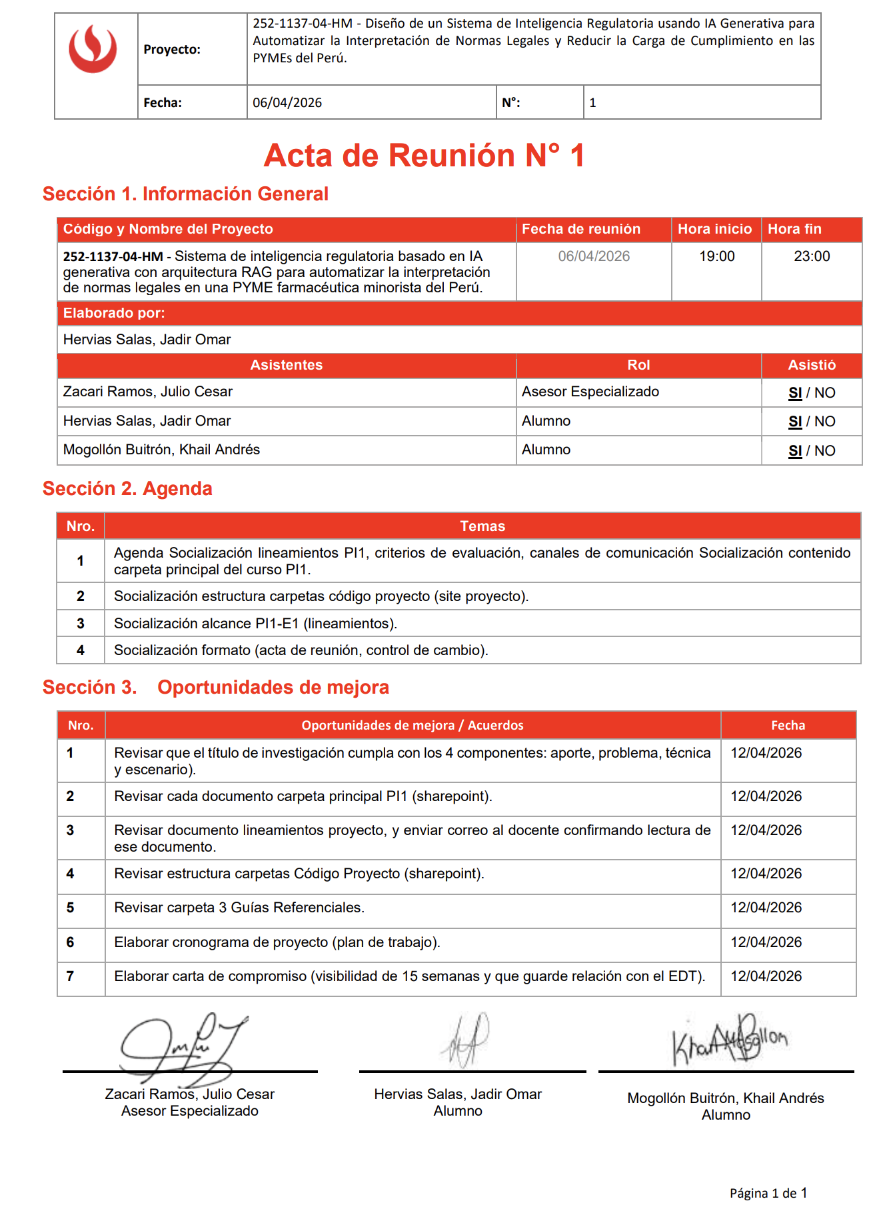
\includegraphics[width=5.65528in,height=7.80785in]{figuras/docx_image40.png}

\subsubsection{Anexo -- Acta de Reunión
2}\label{anexo-acta-de-reuniuxf3n-2}

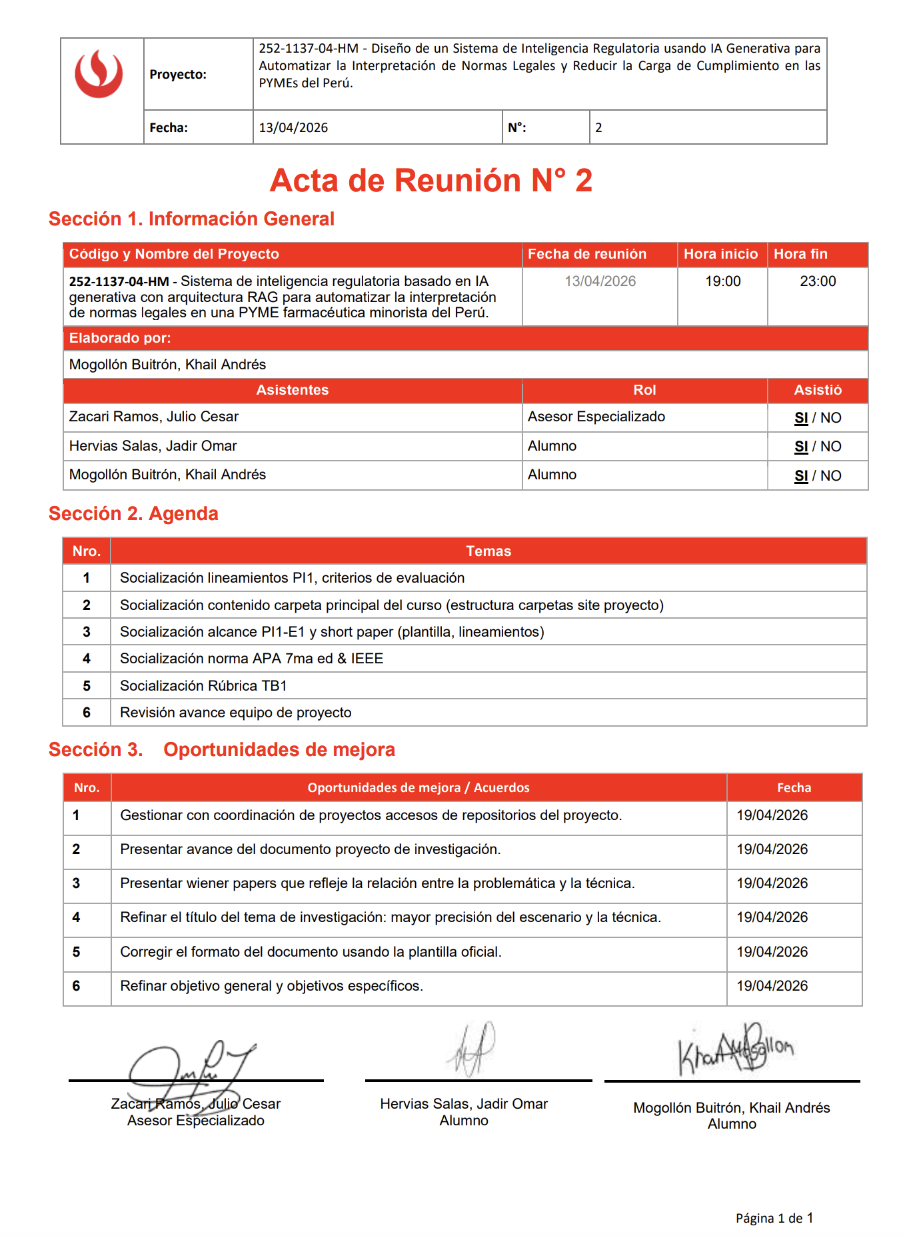
\includegraphics[width=5.74999in,height=7.87444in]{figuras/docx_image41.png}

\subsubsection{Anexo -- Acta de Reunión
3}\label{anexo-acta-de-reuniuxf3n-3}

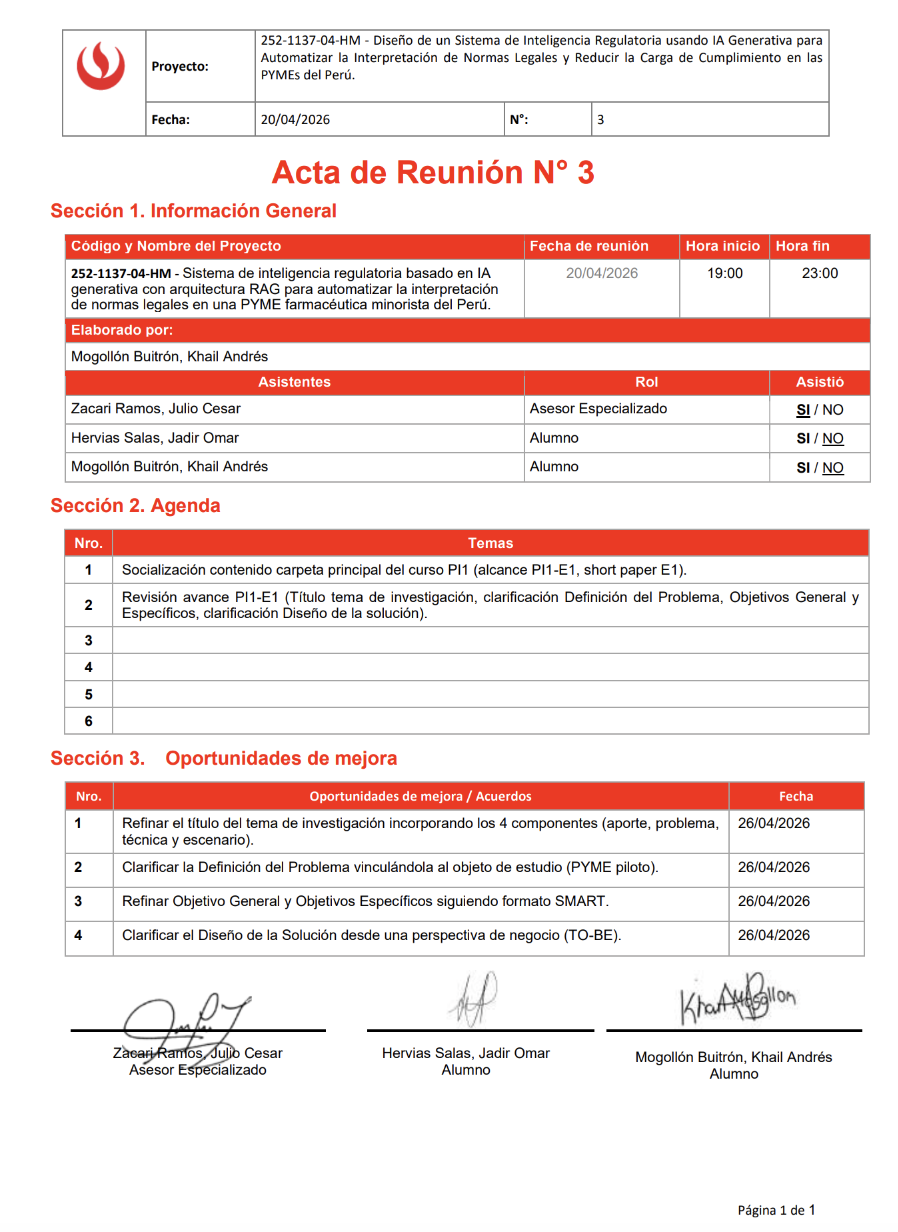
\includegraphics[width=5.66366in,height=7.77019in]{figuras/docx_image42.png}

\subsubsection{Anexo -- Acta de Reunión
4}\label{anexo-acta-de-reuniuxf3n-4}

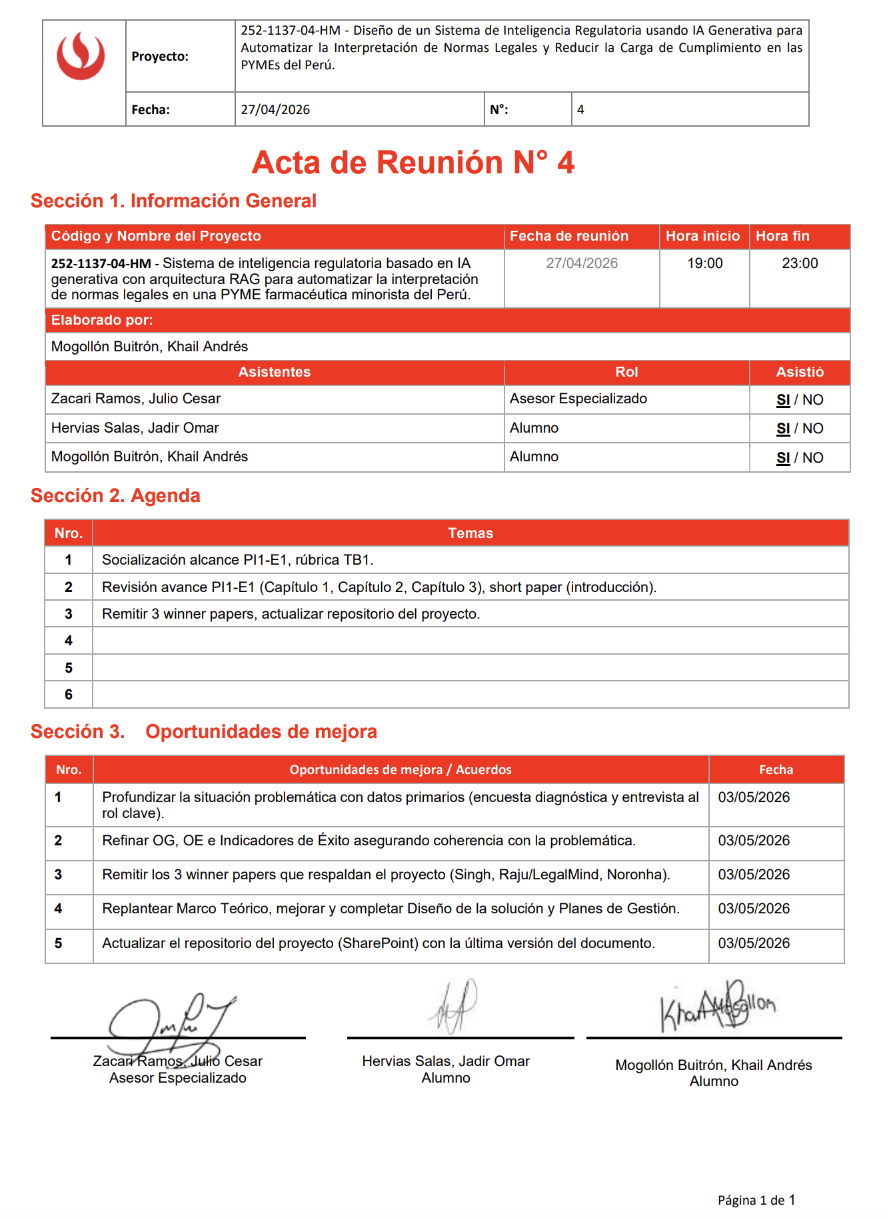
\includegraphics[width=5.25911in,height=7.22535in]{figuras/docx_image43.png}

\subsubsection{Anexo -- Acta de Reunión
5}\label{anexo-acta-de-reuniuxf3n-5}

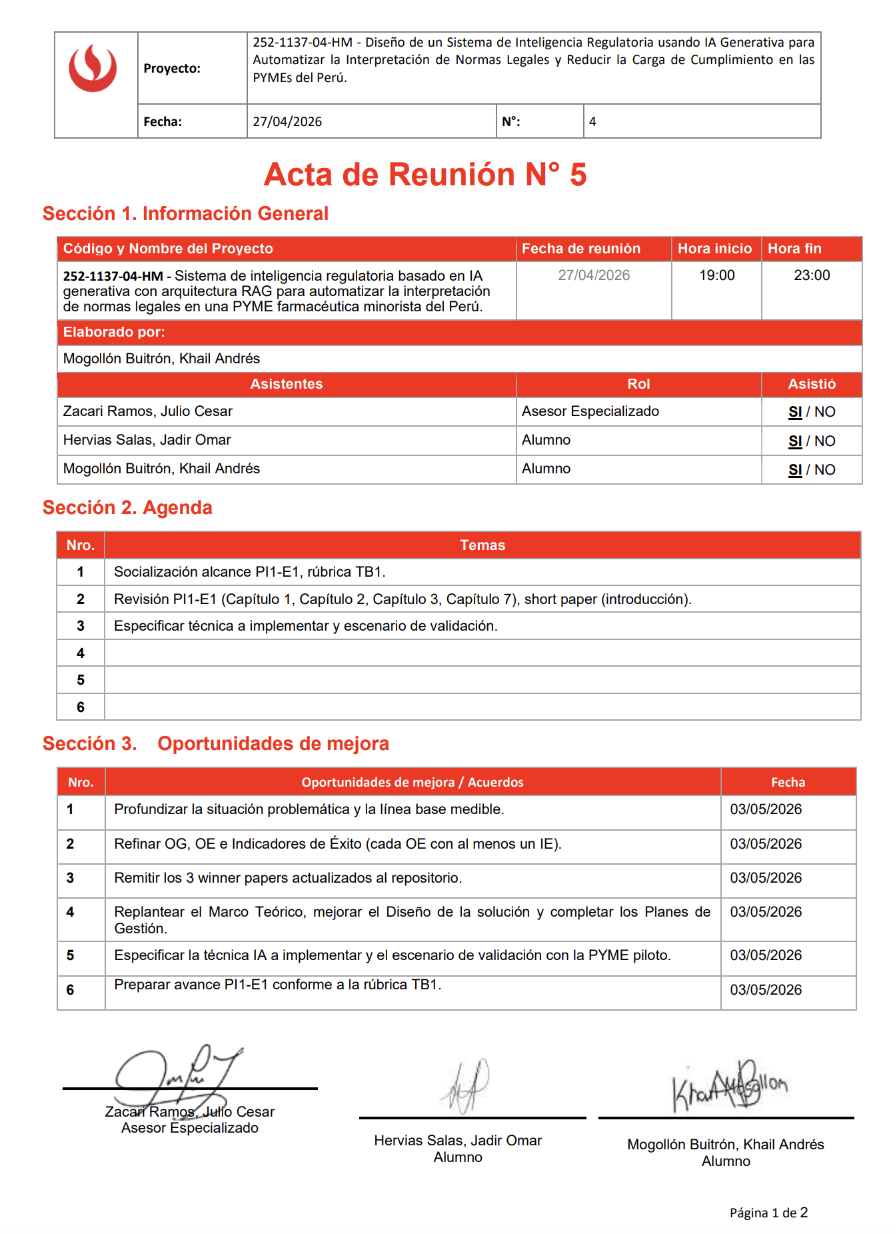
\includegraphics[width=5.62066in,height=7.74095in]{figuras/docx_image44.png}

\subsubsection{Anexo -- Acta de Reunión
6}\label{anexo-acta-de-reuniuxf3n-6}

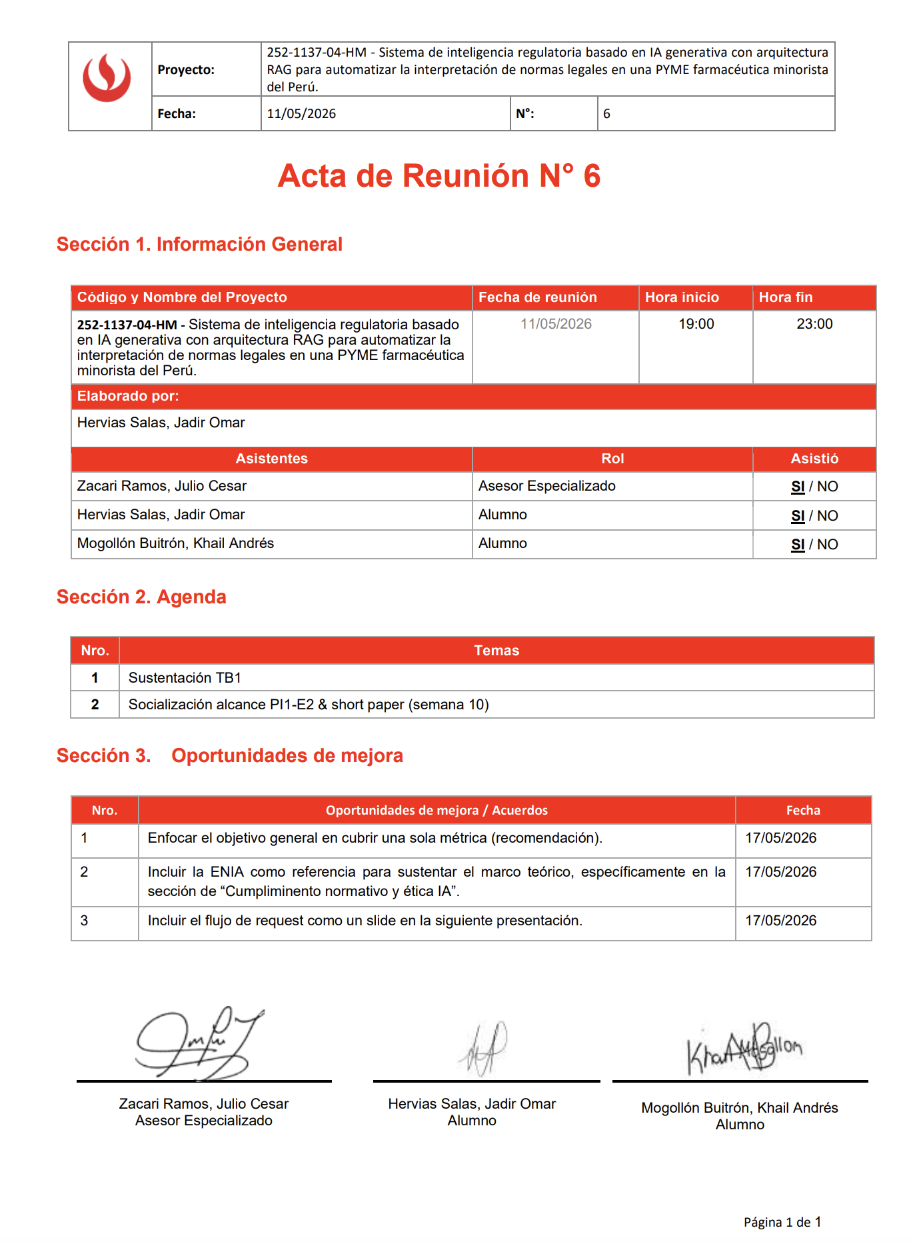
\includegraphics[width=5.99195in,height=8.16009in]{figuras/docx_image45.png}

\subsubsection{Anexo -- Acta de Reunión
7}\label{anexo-acta-de-reuniuxf3n-7}

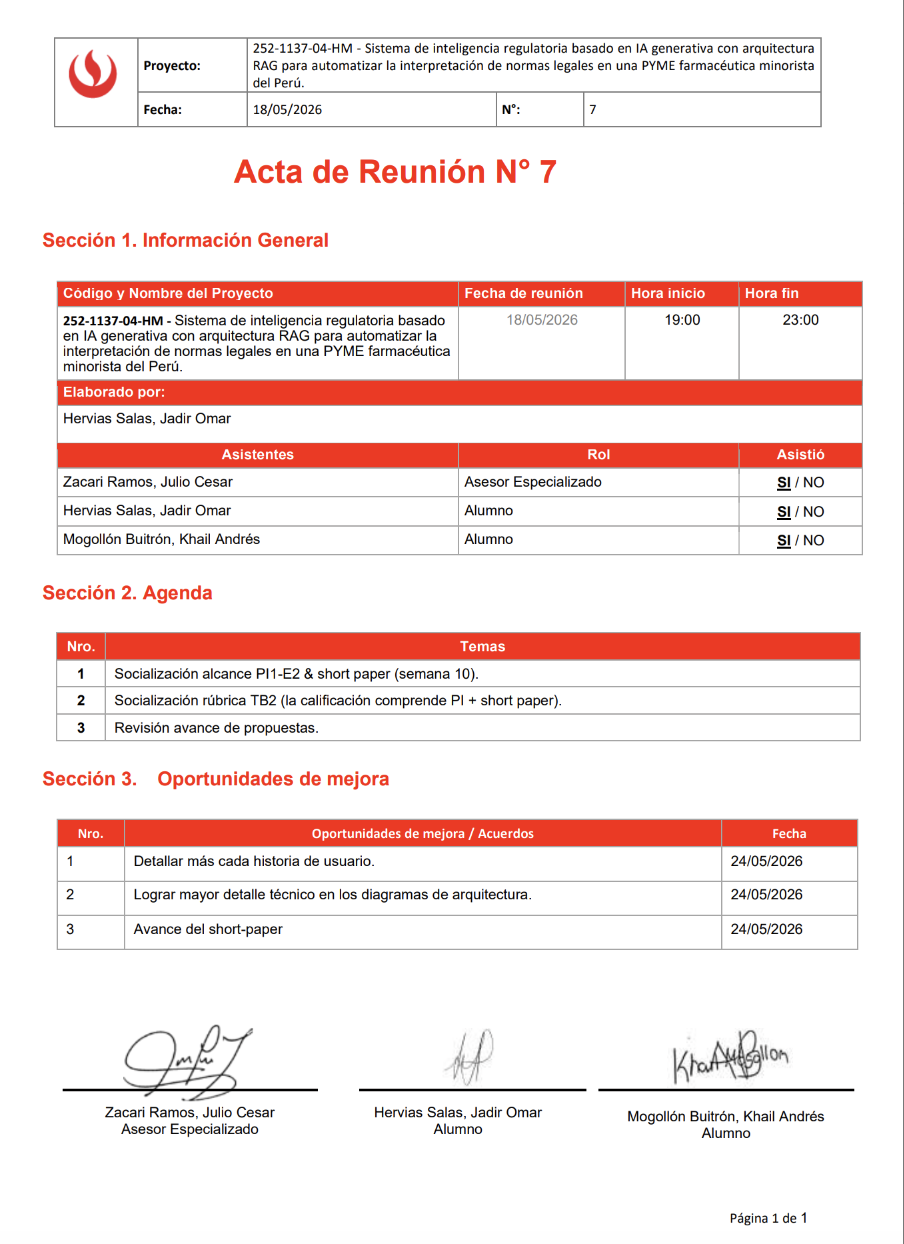
\includegraphics[width=5.80077in,height=7.98248in]{figuras/docx_image46.png}

\subsubsection{Anexo -- Acta de Reunión
9}\label{anexo-acta-de-reuniuxf3n-9}

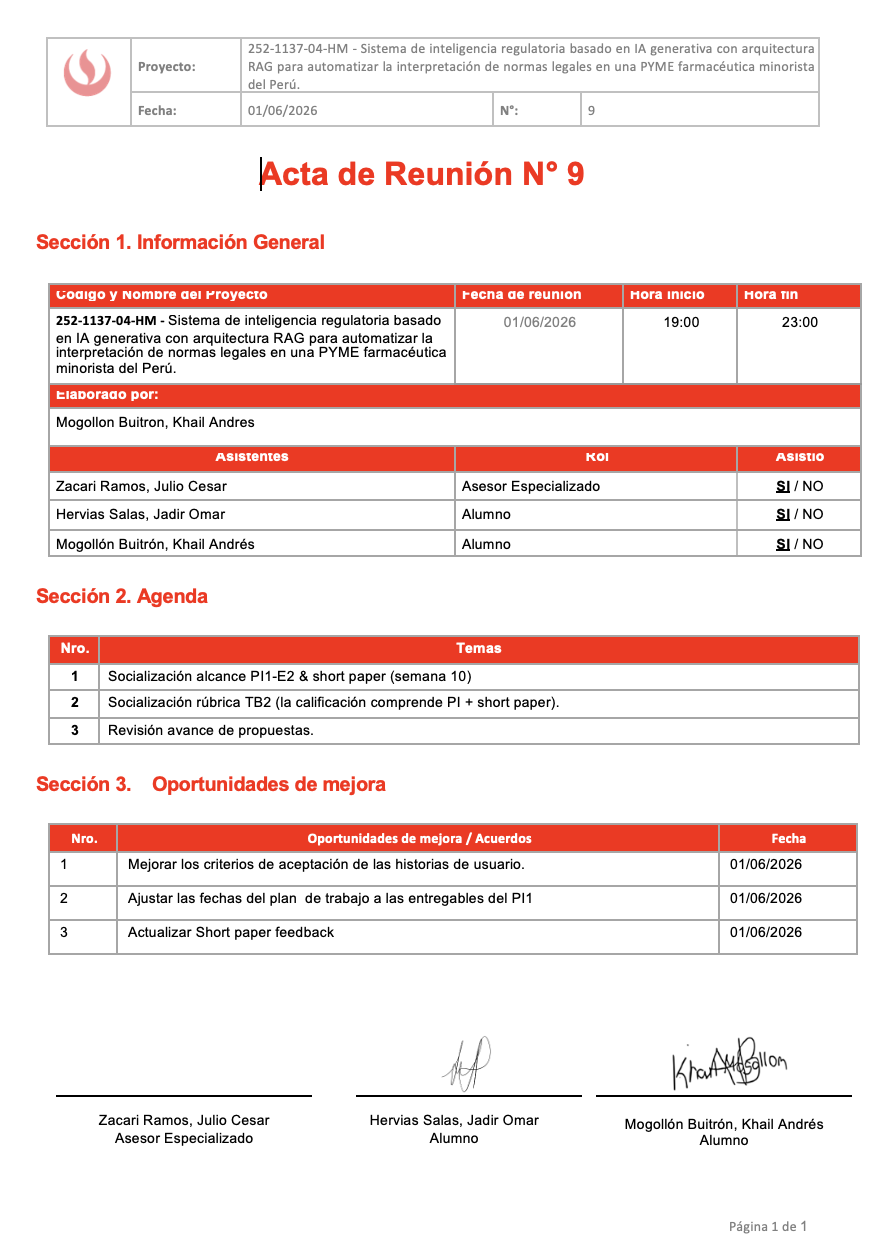
\includegraphics[width=5.55256in,height=7.8161in]{figuras/docx_image47.png}

\subsubsection{Anexo -- Acta de Sprint Planning
-- Sprint
1}\label{anexo-acta-de-sprint-planning-sprint-1}

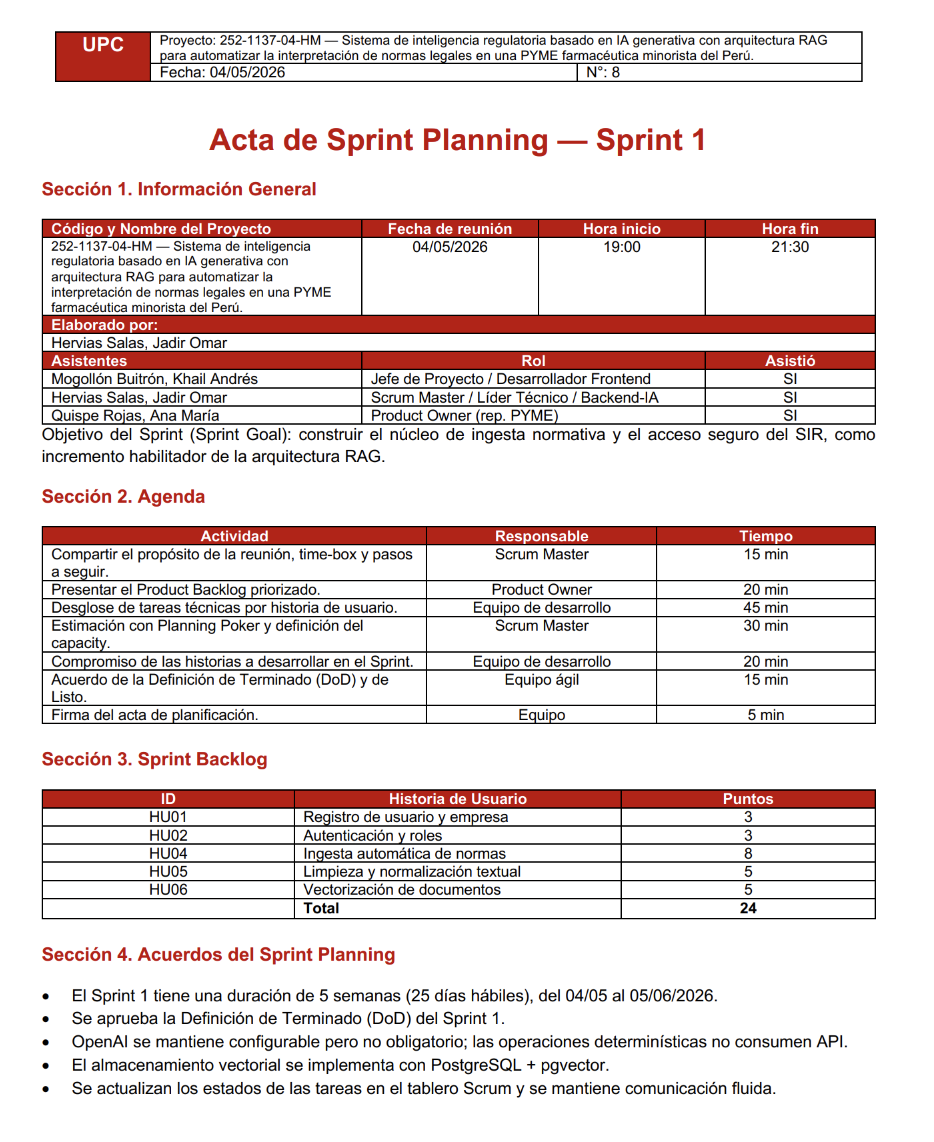
\includegraphics[width=5.6955in,height=6.96388in]{figuras/docx_image48.png}

\includegraphics[width=5.5in,height=1.19444in]{figuras/docx_image49.png}

\subsubsection{Anexo -- Acta de Daily Meeting --
Sprint
1}\label{anexo-acta-de-daily-meeting-sprint-1}

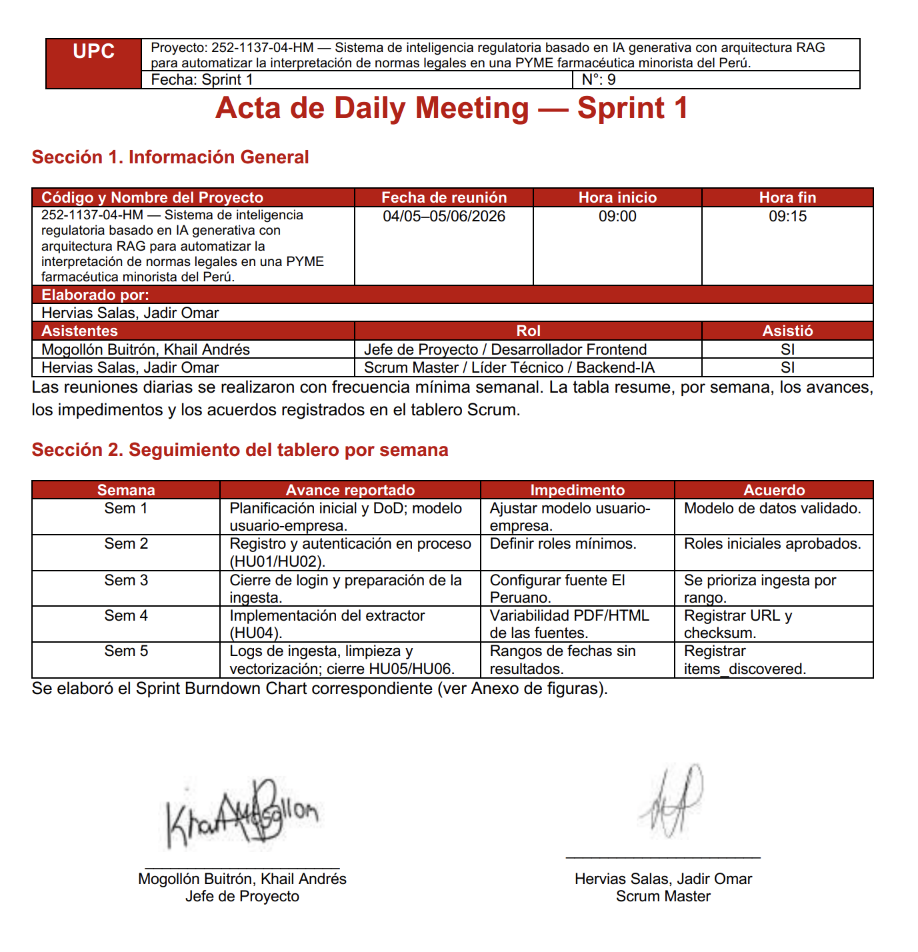
\includegraphics[width=6.375in,height=6.61111in]{figuras/docx_image50.png}

\subsubsection{Anexo -- Acta de Sprint Review--
Sprint
1}\label{anexo-acta-de-sprint-review-sprint-1}

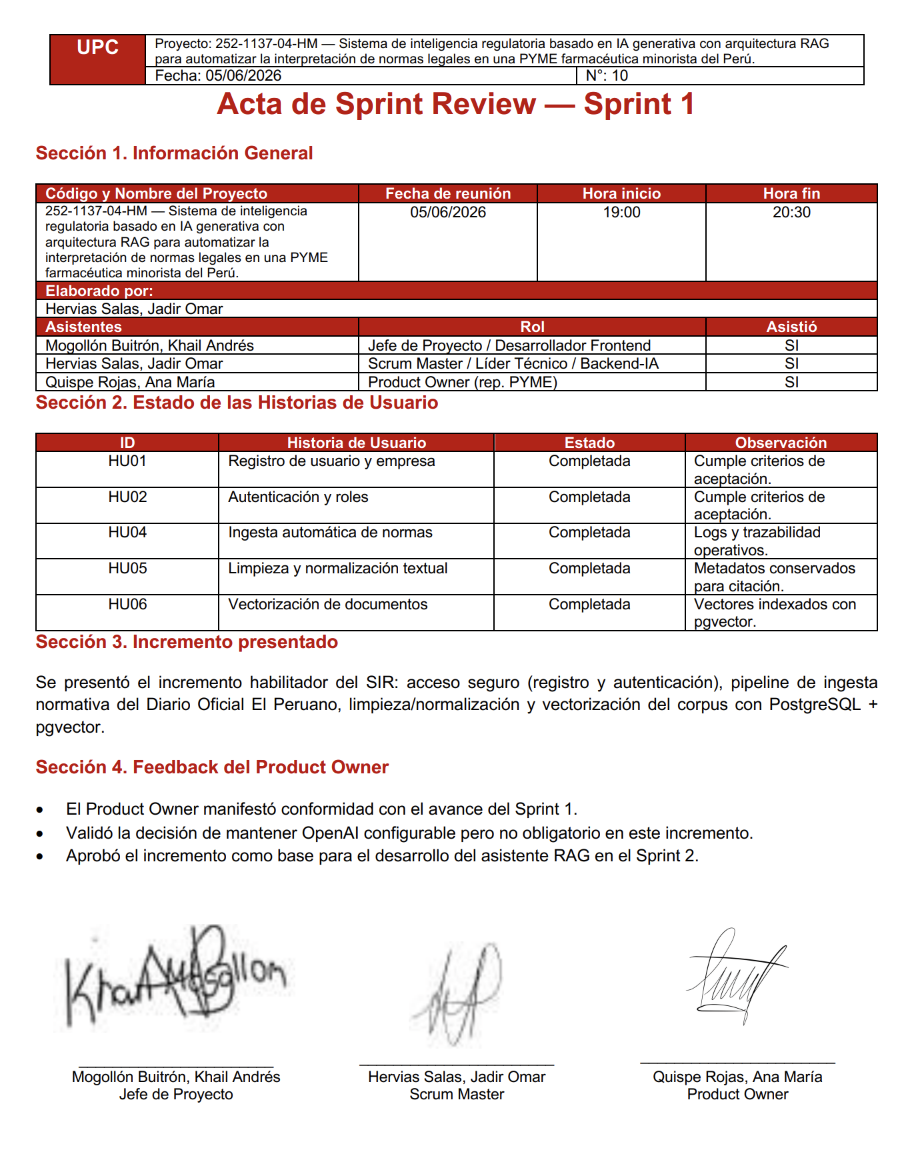
\includegraphics[width=6.43056in,height=7.40278in]{figuras/docx_image2.png}

\subsubsection{Anexo -- Acta de Sprint
Retrospective -- Sprint
1}\label{anexo-acta-de-sprint-retrospective-sprint-1}

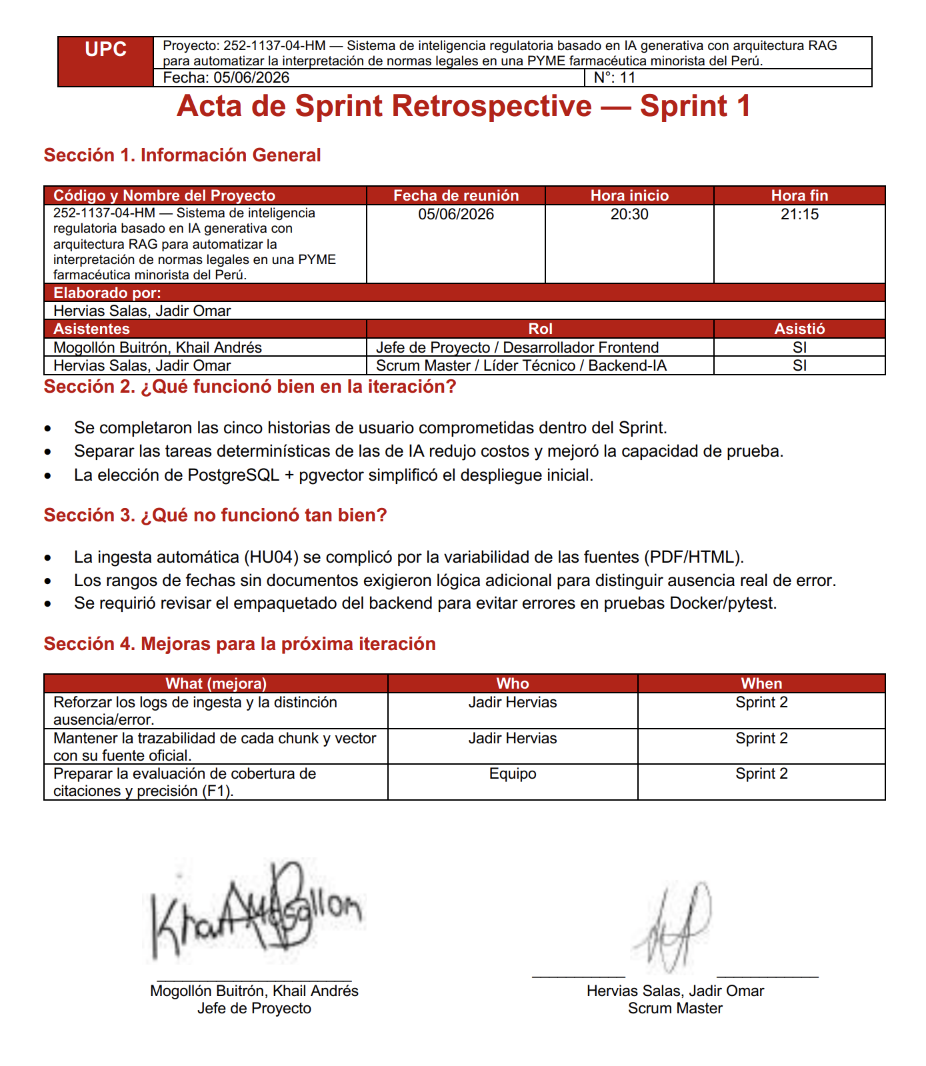
\includegraphics[width=6.43056in,height=7.40278in]{figuras/docx_image51.png}

\end{document}
